\documentclass[11pt]{article}
\usepackage[a4paper,margin=24mm]{geometry}
\usepackage{amsmath,amssymb,amsthm,mathtools}
\numberwithin{equation}{section}
\usepackage[T1]{fontenc}
\usepackage{lmodern}
\PassOptionsToPackage{dvipsnames}{xcolor}
\usepackage{tikz}
\usetikzlibrary{positioning,arrows.meta}
\usepackage{enumitem}
\usepackage{booktabs,longtable,array}
% Motivating paragraphs; set \motiv to \textcolor{Blue}{#1} to highlight them while vetting.
\newcommand{\motiv}[1]{#1}
% Editions. LinearAQFT.tex typesets the full notes; LinearAQFT-Dimock.tex defines
% \AQFTDimockEdition and inputs this file, and typesets only what the verification of Dimock's
% axioms for the free field needs. Material outside that (the lattice field, Huygens' principle,
% illustrations) is in the environment `extra` (on lines of their own) or in \extraonly{...};
% \dimockonly{...} is text for the Dimock edition alone.
\newif\ifdimockedition
\ifdefined\AQFTDimockEdition\dimockeditiontrue\fi
\usepackage{comment}
\ifdimockedition\excludecomment{extra}\else\includecomment{extra}\fi
\newcommand{\extraonly}[1]{\ifdimockedition\else#1\fi}
\newcommand{\dimockonly}[1]{\ifdimockedition#1\fi}
\usepackage[hidelinks]{hyperref}
\newtheorem{theorem}{Theorem}[section]
\newtheorem{proposition}[theorem]{Proposition}
\newtheorem{lemma}[theorem]{Lemma}
\newtheorem{corollary}[theorem]{Corollary}
\theoremstyle{definition}
\newtheorem{definition}[theorem]{Definition}
\newtheorem{example}[theorem]{Example}
\theoremstyle{remark}
\newtheorem{remark}[theorem]{Remark}
\theoremstyle{plain}
\newcommand{\R}{\mathbb R}
\newcommand{\C}{\mathbb C}
\newcommand{\Z}{\mathbb Z}
\newcommand{\ii}{\mathrm i}
\newcommand{\cA}{\mathcal A}
\newcommand{\cR}{\mathcal R}
\newcommand{\alg}{\operatorname{alg}}
\newcommand{\calg}{\overline{\operatorname{alg}}}
\newcommand{\dep}{\mathrel{\triangleleft}}
\newcommand{\Aut}{\operatorname{Aut}}
\newcommand{\CCR}{\operatorname{CCR}}
\newcommand{\cD}{\mathcal D}
\newcommand{\cF}{\mathcal F}
\DeclareMathOperator{\supp}{supp}
% Passages for the user to vet; set to {#1} once accepted.
\newcommand{\vet}[1]{#1}
\newcommand{\vetsource}[1]{#1}  % awaits a check against the source
% Revisions after the oral examination of 26 Sep 2026; set to {#1} once the user accepts them.
\newcommand{\rev}[1]{#1}  % accepted by the user, 26 Sep 2026
% Terminology revision of 26 Sep 2026 (standard terms; citations for credit); set to {#1} once accepted.
\newcommand{\revb}[1]{#1}  % accepted by the user, 27 Sep 2026
% Revisions after the oral examination of milestone C (26 Sep 2026); set to {#1} once accepted.
\newcommand{\revc}[1]{#1}  % accepted by the user, 27 Sep 2026
% Additions from the chapter-by-chapter reading of 27 Sep 2026; set to {#1} once accepted.
\newcommand{\revd}[1]{#1}  % accepted by the user, 27 Sep 2026
% Milestone E2 (chapter 5 and its oral exam, 27 Sep 2026); set to {#1} once accepted.
\newcommand{\reve}[1]{#1}  % accepted by the user, 27 Sep 2026
% Milestone D1 (chapter 6 and its oral exam, 27 Sep 2026); set to {#1} once accepted.
\newcommand{\revf}[1]{#1}  % accepted by the user, 27 Sep 2026
% Milestone D1 whole-document meaning pass (27 Sep 2026); set to {#1} once accepted.
\newcommand{\revg}[1]{#1}  % accepted by the user, 27 Sep 2026
% Stage F (chapter 7 and its oral exam, 28 Sep 2026); set to {#1} once accepted.
\newcommand{\revh}[1]{#1}  % accepted by the user, 28 Sep 2026
% Stage F whole-document meaning pass (28 Sep 2026); set to {#1} once accepted.
\newcommand{\revi}[1]{#1}  % accepted by the user, 28 Sep 2026
% Stage G (chapter 8, its oral exam and the closed-supports amendment, 29 Sep 2026).
\newcommand{\revj}{\relax}  % accepted by the user, 29 Sep 2026
\newcommand{\revjt}[1]{#1}  % accepted by the user, 29 Sep 2026
% Stage G whole-document meaning pass (29 Sep 2026); set to {#1} once accepted.
\newcommand{\revk}[1]{#1}  % accepted by the user, 29 Sep 2026 (after an exposition read)
% Stage H (chapter 9, the Klein--Gordon field, 30 Sep 2026).
\newcommand{\revl}{\relax}  % accepted by the user, 30 Sep 2026
\newcommand{\revlt}[1]{#1}  % accepted by the user, 30 Sep 2026
% Closing pass of the programme (30 Sep 2026); set to {#1} once accepted.
\newcommand{\revm}[1]{#1}  % accepted by the user, 30 Sep 2026
\newcommand{\revtag}[1]{#1}  % tag explanation standardized, 13 Oct 2026; accepted by the user, 13 Oct 2026
% Dependency sentence for the Dimock slices (cloud session, 30 Sep 2026; approved in an earlier
% wording, revised after merging the closing pass); set to {#1} once accepted.
\newcommand{\revn}[1]{#1}  % accepted by the user, 30 Sep 2026
\newcommand{\revo}[1]{#1}  % notes pass of 1 Oct 2026; accepted by the user, 1 Oct 2026
\title{Algebraic quantum field theory of linear fields\dimockonly{\\[4pt]\large The axioms of Dimock for the free scalar field}}
\author{}
\date{}
% Navigation only; checked labels are maintained with reviewed correspondence.
\definecolor{AQFTTagFill}{HTML}{EEEAF8}
\definecolor{AQFTTagBorder}{HTML}{D6CEEB}
\definecolor{AQFTTagText}{HTML}{5B477D}
\newcommand{\AQFTLeanTag}{%
  \tikz[baseline=(tag.base)]\node[rounded corners=1.5pt,
    fill=AQFTTagFill,draw=AQFTTagBorder,text=AQFTTagText,
    line width=0.3pt,inner xsep=3pt,inner ysep=1.5pt] (tag)
    {\normalfont\scriptsize\sffamily Lean\,\ensuremath{\checkmark}};}
\definecolor{AQFTArtFill}{HTML}{F2F2F2}
\definecolor{AQFTArtBorder}{HTML}{BDBDBD}
\definecolor{AQFTArtText}{HTML}{555555}
\newcommand{\AQFTArtefactTag}{%
  \tikz[baseline=(tag.base)]\node[rounded corners=1.5pt,
    fill=AQFTArtFill,draw=AQFTArtBorder,text=AQFTArtText,dashed,
    line width=0.3pt,inner xsep=3pt,inner ysep=1.5pt] (tag)
    {\normalfont\scriptsize\sffamily formalization};}
\newcommand{\artefact}[1]{#1\nobreak\hspace{0.3em}\AQFTArtefactTag}
% Status tags for examples without a reviewed Lean counterpart: script ✓ (exhaustively
% verified by a check script) and paper (checked on paper only).
\definecolor{AQFTScrFill}{HTML}{E8F3EC}
\definecolor{AQFTScrBorder}{HTML}{BFDCC9}
\definecolor{AQFTScrText}{HTML}{2F6B45}
\newcommand{\AQFTScriptTag}{%
  \tikz[baseline=(tag.base)]\node[rounded corners=1.5pt,
    fill=AQFTScrFill,draw=AQFTScrBorder,text=AQFTScrText,
    line width=0.3pt,inner xsep=3pt,inner ysep=1.5pt] (tag)
    {\normalfont\scriptsize\sffamily script\,\ensuremath{\checkmark}};}
\definecolor{AQFTPapFill}{HTML}{FBF1E3}
\definecolor{AQFTPapBorder}{HTML}{E6CFA8}
\definecolor{AQFTPapText}{HTML}{7A5520}
\newcommand{\AQFTPaperTag}{%
  \tikz[baseline=(tag.base)]\node[rounded corners=1.5pt,
    fill=AQFTPapFill,draw=AQFTPapBorder,text=AQFTPapText,
    line width=0.3pt,inner xsep=3pt,inner ysep=1.5pt] (tag)
    {\normalfont\scriptsize\sffamily paper};}
\makeatletter
\newcommand{\AQFTExampleStatus}[2]{\expandafter\gdef\csname aqft@status@#1\endcsname{#2}}
\newcommand{\AQFTCheckedLabel}[1]{\expandafter\gdef\csname aqft@checked@#1\endcsname{}}
\newcommand{\AQFTEnableLinks}{%
  \let\AQFTOriginalLabel\label
  \renewcommand{\label}[1]{%
    \AQFTOriginalLabel{##1}%
    \ifcsname aqft@checked@##1\endcsname
      \nobreak\hspace{0.4em}\hyperlink{lean:##1}{\AQFTLeanTag}%
    \else\ifcsname aqft@status@##1\endcsname
      \nobreak\hspace{0.4em}\AQFTStatusTag{\csname aqft@status@##1\endcsname}%
    \fi\fi}}
\def\aqft@script{script}\def\aqft@paper{paper}
\newcommand{\AQFTStatusTag}[1]{\edef\aqft@s{#1}%
  \ifx\aqft@s\aqft@script\AQFTScriptTag\else\ifx\aqft@s\aqft@paper\AQFTPaperTag\fi\fi}
\makeatother

% Labels whose Lean correspondence has been independently reviewed (added after the fidelity
% review of each milestone; see README.md).
\AQFTCheckedLabel{lem:commute}
\AQFTCheckedLabel{prop:generated}
\AQFTCheckedLabel{lem:pairs}
\AQFTCheckedLabel{ex:two-qubits}
\AQFTCheckedLabel{ex:nilpotent}
\AQFTCheckedLabel{lem:weyl-isometry}
\AQFTCheckedLabel{prop:weyl-relation}
\AQFTCheckedLabel{prop:weyl-unitary}
\AQFTCheckedLabel{lem:weyl-system}
\AQFTCheckedLabel{prop:ccr-system}
\AQFTCheckedLabel{prop:relabel}
\AQFTCheckedLabel{prop:right-weyl}
\AQFTCheckedLabel{prop:vector-state}
\AQFTCheckedLabel{ex:lattice-index}
\AQFTCheckedLabel{lem:kg-symmetric}
\AQFTCheckedLabel{lem:kernel}
\AQFTCheckedLabel{lem:unique}
\AQFTCheckedLabel{prop:green}
\AQFTCheckedLabel{prop:commutator}
\AQFTCheckedLabel{thm:lattice-timeslice}
\AQFTCheckedLabel{cor:lattice-dep}
\AQFTCheckedLabel{lem:phase-iso}
\AQFTCheckedLabel{thm:weyl-net}
\AQFTCheckedLabel{thm:weyl-cov}
\AQFTCheckedLabel{cor:weyl-iso}
\AQFTCheckedLabel{thm:ccr-cov}
% Milestone E2 (fidelity review PASS WITH MINOR, 27 Sep 2026).
\AQFTCheckedLabel{ex:lattice-phase}
\AQFTCheckedLabel{prop:lattice-data}
\AQFTCheckedLabel{prop:lattice-nondeg}
\AQFTCheckedLabel{ex:lattice-nonvacuous}
\AQFTCheckedLabel{lem:lattice-cov-E}
\AQFTCheckedLabel{prop:lattice-iso}
\AQFTCheckedLabel{thm:lattice-net}
\AQFTCheckedLabel{prop:pullback}
\AQFTCheckedLabel{lem:two-slices}
\AQFTCheckedLabel{thm:cauchy-map}
\AQFTCheckedLabel{thm:cauchy-net}
\AQFTCheckedLabel{prop:leapfrog}
% Milestone D1 (fidelity review PASS, 27 Sep 2026).
\AQFTCheckedLabel{lem:conj}
\AQFTCheckedLabel{lem:average}
\AQFTCheckedLabel{lem:phases}
\AQFTCheckedLabel{lem:generic}
\AQFTCheckedLabel{prop:approx}
\AQFTCheckedLabel{lem:faithful}
\AQFTCheckedLabel{thm:simple}
\AQFTCheckedLabel{prop:simple-rep}
\AQFTCheckedLabel{thm:primitive}
\AQFTCheckedLabel{thm:dimock}
\AQFTCheckedLabel{cor:lattice-dimock}
% Stage F (fidelity review PASS, 28 Sep 2026).
\AQFTCheckedLabel{lem:green-index}
\AQFTCheckedLabel{lem:green-E}
\AQFTCheckedLabel{prop:green-phase}
\AQFTCheckedLabel{prop:green-nondeg}
\AQFTCheckedLabel{thm:green-axioms}
\AQFTCheckedLabel{prop:green-symmetry}
\AQFTCheckedLabel{prop:lattice-green}
\AQFTCheckedLabel{thm:lattice-green-compare}
\AQFTCheckedLabel{prop:lattice-green-translate}
% Stage F amendment, pointwise dependence (fidelity review PASS, 28 Sep 2026): the amended
% declarations behind ex:lattice-index,
% ex:lattice-aut, cor:lattice-dep, ex:lattice-phase, prop:lattice-data, ex:lattice-nonvacuous,
% prop:lattice-iso, lem:green-index, prop:green-phase, prop:green-symmetry and
% thm:lattice-green-compare were re-reviewed; the marks above stand.
% Examples: status script or paper (a Lean-checked example uses \AQFTCheckedLabel instead).
\AQFTExampleStatus{ex:gh-index}{paper}
\AQFTExampleStatus{ex:lattice-aut}{paper}
\AQFTExampleStatus{ex:one-dof}{paper}
\AQFTExampleStatus{ex:sigma-zero}{paper}
\AQFTExampleStatus{ex:lattice-witness}{script}  % check_e2.py, closing pass 30 Sep 2026
% Stage G (Chapter 8): the G1-G4 fidelity reviews and the chapter audit.
\AQFTCheckedLabel{prop:mink-basic}
\AQFTCheckedLabel{prop:kirchhoff}
\AQFTCheckedLabel{thm:mink-core}
\AQFTCheckedLabel{cor:mink-green}
\AQFTCheckedLabel{lem:mink-compact}
\AQFTCheckedLabel{prop:mink-cutoff}
\AQFTCheckedLabel{thm:mink-green}
\AQFTCheckedLabel{thm:mink-unique}
\AQFTCheckedLabel{lem:mink-lorentz}
\AQFTCheckedLabel{prop:mink-symmetry}
\AQFTCheckedLabel{thm:mink-covariance}
% Stage H (Chapter 9): the H1-H4 fidelity reviews and the chapter audit.
\AQFTCheckedLabel{lem:kg-ibp}
\AQFTCheckedLabel{thm:kg-greenops}
\AQFTCheckedLabel{prop:kg-wave}
\AQFTCheckedLabel{lem:kg}
\AQFTCheckedLabel{lem:kg-causal}
\AQFTCheckedLabel{lem:kg-cutoff}
\AQFTCheckedLabel{prop:kg-ext}
\AQFTCheckedLabel{lem:kg-power}
\AQFTCheckedLabel{cor:kg-iterate}
\AQFTCheckedLabel{prop:kg-adj}
\AQFTCheckedLabel{lem:kg-linear}
\AQFTCheckedLabel{prop:kg-conv}
\AQFTCheckedLabel{prop:kg-smooth}
\AQFTCheckedLabel{thm:kg-green-id}
\AQFTCheckedLabel{prop:kg-supp}
\AQFTCheckedLabel{prop:kg-adv}
\AQFTCheckedLabel{prop:kg-series-adj}
\AQFTCheckedLabel{thm:kg-field}
\AQFTCheckedLabel{cor:kg-zero}
\AQFTCheckedLabel{prop:kg-huygens}
\AQFTCheckedLabel{lem:kg-pos}
\AQFTCheckedLabel{prop:kg-pos2}
\AQFTCheckedLabel{lem:kg-tail}
\AQFTCheckedLabel{lem:kg-dil}
\AQFTCheckedLabel{thm:kg-fail}
\AQFTCheckedLabel{thm:kg-iff}

\begin{document}
\AQFTEnableLinks
\sloppy
\maketitle
\vspace{-2em}
\noindent\motiv{In algebraic quantum field theory~\cite{haagkastler} the observables measurable in a region $O$
of spacetime form a C*-algebra $\cA(O)$. \revc{The observables are taken bounded, such as the exponentials
$e^{\ii\phi(f)}$ of smeared fields rather than the unbounded fields $\phi(f)$, which avoids
questions of domains; closing in norm makes each $\cA(O)$ a C*-algebra\revd{, which for the free
field is determined by the canonical commutation relations up to isomorphism, independently of the
Hilbert space (Remark~\ref{rem:weyl-covariance})}.}}

\motiv{These algebras sit inside one another: larger regions have larger algebras, algebras of spacelike separated
regions commute, and the algebra of a region is already contained in the algebra of any
region that determines it causally. Dimock~\cite{dimock} formulated these requirements for a
Lorentzian manifold as five axioms and verified them for the free scalar field on a globally
hyperbolic spacetime. \revm{These notes give a formalized version of that verification} \revo{in an abstract form: the spacetime enters only through the Green data described next, primitivity is proved given an irreducible representation, and Dimock's form of the time-slice axiom follows on paper}\revm{.}}

\motiv{\revm{The analysis the verification rests on is the existence of retarded and advanced Green
operators for the Klein--Gordon operator, a theorem of hyperbolic partial differential
equations~\cite{bgp}. Here it enters as a hypothesis, the Green data of Chapter~\ref{sec:green},
modelled on the Green-hyperbolic operators of~\cite{baer-green}. The hypothesis is proved \extraonly{on a
lattice spacetime, the running example (Chapters~\ref{sec:lattice} and~\ref{sec:latticenet}), }for
the free massless field on $3+1$ Minkowski space (Chapter~\ref{sec:minkowski}), and for the
Klein--Gordon field there with any real $m^2$, negative values included (Chapter~\ref{sec:mass}).}}

{\small\tableofcontents}
\medskip

\section*{About these notes}
\noindent\motiv{\revm{These notes are the mathematical account of the Lean library LinearAQFT and the
blueprint from which it was built. The library depends on Mathlib, on LocalAlgebrasLean, which
holds regions with their orthogonality and nets of local algebras, and on BosonicLean, which holds
the CCR algebra, Weyl systems, their relabelling and pullback, the simplicity theorem, irreducible
representations and primitivity; the
declaration index at the end names the declarations of LinearAQFT and BosonicLean.}}

\medskip
\noindent\motiv{\revm{\textbf{Terminology.} Standard terms keep their usual meaning: net of local
algebras; Weyl operator; Weyl system (here required to generate its algebra); CCR algebra; vector
state; retarded and advanced Green operators; \extraonly{commutator function; }causal propagator; Cauchy
surface; globally hyperbolic; Cauchy temporal function; Green-hyperbolic
operator~\cite{baer-green}; the retarded potential; spherical means; orthochronous Lorentz and
Poincar\'e maps; the Klein--Gordon operator; local operators; the tachyonic case\extraonly{; chronological
order; Huygens' principle}. The axioms are those of~\cite[p.~220]{dimock}: Axioms~1--3 (isotony
with generation, primitivity, causality) are essentially the Haag--Kastler
axioms~\cite{haagkastler}, Axiom~4 (time slice) goes back to Haag and
Schroer~\cite{haag-schroer}, and Axiom~5 is covariance. Results of~\cite{dimock} are
cited by their numbers there, for example Axiom~4 or Theorem~4 of~\cite{dimock}.}}

\medskip
\noindent\motiv{\revm{The \emph{time-slice property} is condition (N3) of
Definition~\ref{def:axioms} for the causal index at hand; the \emph{time-slice axiom} is Axiom~4
of~\cite{dimock}, (N3) for the dependence of Example~\ref{ex:gh-index}. For Green data the first is
proved (\revo{Proposition~\ref{prop:green-phase} and Theorem~\ref{thm:weyl-net}}). \revo{On paper it implies the second for the Green data of Remark~\ref{rem:green-continuum}, whose cutoffs are given by all Cauchy temporal functions (Remark~\ref{rem:green-dep-spacetime}), and for the instances of Chapters~\ref{sec:minkowski} and~\ref{sec:mass}, whose cutoffs are inertial slabs, when the Cauchy surface is flat. For a curved Cauchy surface that implication can fail, and the axiom then rests on all Cauchy temporal functions as cutoffs, which are not formalized (Remark~\ref{rem:mink-slabs}).}}}

\medskip
\noindent\motiv{\revm{\textbf{Coined terms.} These terms are coined for these notes and defined where
they first appear: causal index (Definition~\ref{def:causal-index}); covariance pair
(Definition~\ref{def:covariance}); family of generators and generated net
(Definition~\ref{def:generated}); relabelling unitary (Definition~\ref{def:relabel}); right Weyl
operator (Definition~\ref{def:right-weyl}); phase-space data (Definition~\ref{def:phase-space}); the
net of a Weyl system (Definition~\ref{def:weyl-net}); the CCR net (Definition~\ref{def:ccr-net});
\extraonly{the pullback of a Weyl system (Definition~\ref{def:pullback}); the Cauchy map
(Definition~\ref{def:cauchy-map}); the Cauchy-data net (Definition~\ref{def:cauchy-net}); }the
average $\mathsf M^u_n$ (Definition~\ref{def:average}); Green data with their Green identities
$PG^\pm f=f$, $G^\pm P_\cD f=f$ (not Green's identities of vector calculus), cutoffs and slabs
(Definition~\ref{def:green-data}); the derived causal index (Definition~\ref{def:green-index}); the
derived phase-space data (Definition~\ref{def:green-phase}); a symmetry of Green data
(Definition~\ref{def:green-symmetry}); the future and past cone measures
(Definition~\ref{def:kirchhoff}); future unit vectors and inertial slabs
(Definition~\ref{def:mink-cutoff}); the extended Green operators and functions supported in the
future or past of a compact set (Definition~\ref{def:kg-supported}).}}

\medskip
\noindent\motiv{\textbf{Reading conventions.} C*-algebras are unital and complex; a
$*$-homomorphism is unital. For a subset $s$ of a C*-algebra $A$, $\alg(s)$ is the smallest
$*$-subalgebra of $A$ containing $s$, and $\calg(s)$ is its norm closure, the C*-subalgebra
generated by $s$. Subalgebras and $*$-subalgebras contain the unit. Two elements commute when $ab=ba$. Inner
products are linear in the second argument. \revg{$\pi$ and $e$ also keep their numerical
meaning.} $[x=y]$ is $1$ if $x=y$ and $0$ otherwise.}

\medskip
\noindent\motiv{A statement marked
\revtag{\AQFTLeanTag{}} has a checked proof in LinearAQFT\revm{ or in its dependency BosonicLean}
whose correspondence with the statement here has been independently reviewed; the declaration index at the end names the
checked declarations. Every Example carries exactly one status: \AQFTLeanTag{} as above,
\AQFTScriptTag{} when a check script verifies it exhaustively, or \AQFTPaperTag{} when it is
checked on paper only. Definitions, Remarks and paragraphs of motivation carry no marks\revm{; they are
checked on paper, and ``on paper'' in them marks a claim that goes beyond the marked statements they
cite}. A sentence tagged \AQFTArtefactTag{} records a choice made for the formalization that
a proof on paper would not need.}

\section*{Notation}
\noindent \revm{Each row lists symbols and their meanings, with the chapter where each meaning is
defined in parentheses; a second meaning of a symbol is used only in the place its row names.}
{\small
\ifdimockedition\def\notationfile{notation-dimock}\else\def\notationfile{notation-full}\fi
\begin{longtable}{@{}l>{\raggedright\arraybackslash}p{0.66\textwidth}@{}}
\input{\notationfile}
\end{longtable}}
\section*{Roadmap}
\addcontentsline{toc}{section}{Roadmap}

\noindent\motiv{\vet{\extraonly{\revd{The lattice appears in Chapter~\ref{sec:nets} as an example;
its propagators (Chapter~\ref{sec:lattice}) come before the general net
(Chapter~\ref{sec:phasespace}), and the lattice net is completed in
\reve{Chapter~\ref{sec:latticenet}}\revg{, apart from primitivity (Chapter~\ref{sec:simple})}.}}\dimockonly{\revm{This
edition contains only what the verification of the axioms of~\cite{dimock} for the free scalar field
needs; the full notes add the lattice field, the net defined through Cauchy data, Huygens' principle
and some illustrations.}}
\revm{Chapter~\ref{sec:nets} states the axioms for any set of regions carrying inclusion,
orthogonality and dependence, and reduces them to properties of generators
(Proposition~\ref{prop:generated}); Chapter~\ref{sec:weyl} constructs the Weyl operators and the CCR
algebra.} Figure~\ref{fig:roadmap} shows which chapters use which.}}

\ifdimockedition
\begin{figure}[ht]
\centering
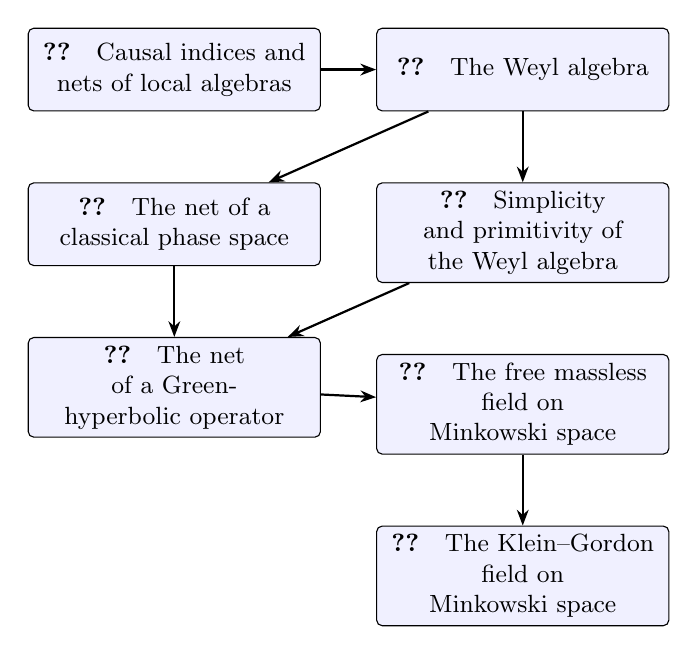
\begin{tikzpicture}[
  font=\small,
  done/.style={draw, rounded corners=2pt, fill=Blue!6, text width=3.5cm, align=center,
    minimum height=1.05cm, inner sep=3pt},
  dep/.style={-{Stealth[length=2mm]}, thick},
  node distance=0.9cm and 0.7cm]
  \node[done] (c1) {\ref*{sec:nets}\quad Causal indices and nets of local algebras};
  \node[done, right=of c1] (c2) {\ref*{sec:weyl}\quad The Weyl algebra};
  \node[done, below=of c1] (c4) {\ref*{sec:phasespace}\quad The net of a classical phase space};
  \node[done, below=of c2] (c6) {\ref*{sec:simple}\quad Simplicity and primitivity of the Weyl algebra};
  \node[done, below=of c4] (c7) {\ref*{sec:green}\quad The net of a Green-hyperbolic operator};
  \node[done, below=of c6] (c8) {\ref*{sec:minkowski}\quad The free massless\\ field on Minkowski space};
  \node[done, below=of c8] (c9) {\ref*{sec:mass}\quad The Klein--Gordon\\ field on Minkowski space};
  \draw[dep] (c1) -- (c2);
  \draw[dep] (c2) -- (c4);
  \draw[dep] (c2) -- (c6);
  \draw[dep] (c4) -- (c7);
  \draw[dep] (c6) -- (c7);
  \draw[dep] (c7) -- (c8);
  \draw[dep] (c8) -- (c9);
\end{tikzpicture}
\caption{\revm{Dependence of the chapters. An arrow means that the later chapter uses the earlier
one; a chapter also uses every chapter from which a chain of arrows leads to it, and arrows
implied by such chains are omitted.}}
\label{fig:roadmap}
\end{figure}
\else
\begin{figure}[ht]
\centering
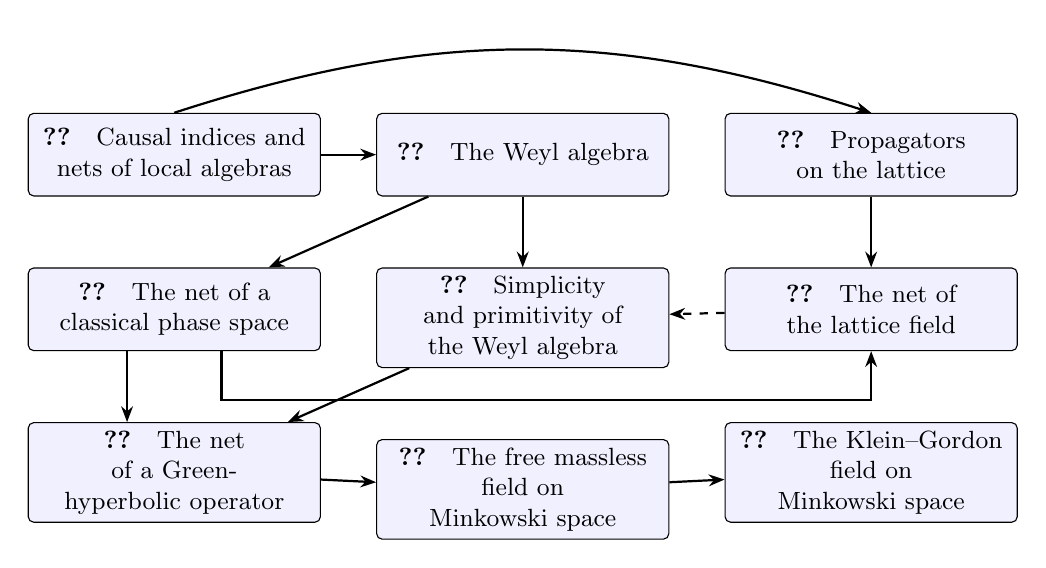
\begin{tikzpicture}[
  font=\small,
  done/.style={draw, rounded corners=2pt, fill=Blue!6, text width=3.5cm, align=center,
    minimum height=1.05cm, inner sep=3pt},
  plan/.style={done, dashed, fill=none},
  dep/.style={-{Stealth[length=2mm]}, thick},
  node distance=0.9cm and 0.7cm]
  \node[done] (c1) {\ref*{sec:nets}\quad Causal indices and nets of local algebras};
  \node[done, right=of c1] (c2) {\ref*{sec:weyl}\quad The Weyl algebra};
  \node[done, right=of c2] (c3) {\ref*{sec:lattice}\quad Propagators on the lattice};
  \node[done, below=of c1] (c4) {\revb{\ref*{sec:phasespace}\quad The net of a classical phase space}};
  \node[done, below=of c2] (c6) {\revf{\ref*{sec:simple}\quad Simplicity and primitivity of the Weyl algebra}};
  \node[done, below=of c3] (c5) {\reve{\ref*{sec:latticenet}\quad The net of the lattice field}};
  \node[done, below=of c4] (c7) {\revh{\ref*{sec:green}\quad The net of a Green-hyperbolic operator}};
  \node[done, below=of c6] (c8) {\revjt{\ref*{sec:minkowski}\quad The free massless\\ field on Minkowski space}};
  \node[done, below=of c5] (c9) {\revlt{\ref*{sec:mass}\quad The Klein--Gordon\\ field on Minkowski space}};
  \draw[dep] (c1) -- (c2);
  \draw[dep] (c1.north) to[bend left=18] (c3.north);
  \draw[dep] (c2) -- (c4);
  \draw[dep, dashed] (c5) -- (c6);
  \draw[dep] (c2) -- (c6);
  \draw[dep] ([xshift=-6mm]c4.south) -- ([xshift=-6mm]c7.north);
  \draw[dep] (c3) -- (c5);
  \draw[dep] ([xshift=6mm]c4.south) -- ++(0,-0.62) -| (c5.south);
  \draw[dep] (c6) -- (c7);
  \draw[dep] (c7) -- (c8);
  \draw[dep] (c8) -- (c9);
\end{tikzpicture}
\caption{Dependence of the chapters. An arrow means that the later chapter uses the earlier
one\revi{; a chapter also uses every chapter from which a chain of arrows leads to it, and arrows
implied by such chains are omitted. Chapter~\ref{sec:simple}, for instance, rests mainly on
Chapter~\ref{sec:weyl}}. \revh{Chapter~\ref{sec:green} constructs the classical phase space from Green data, which gives
the theorem for every instance of Green data, over the derived causal index.} \revc{Chapter~\ref{sec:phasespace} uses Chapter~\ref{sec:lattice} only in its
running example, Example~\ref{ex:lattice-phase}\revo{, and in Remark~\ref{rem:massless-reversal}}.} \revf{Chapter~\ref{sec:simple} uses
Chapters~\ref{sec:phasespace} and~\ref{sec:latticenet} only in} \revg{Remark~\ref{rem:irrep} and} \revf{its last section.} \revh{Chapter~\ref{sec:green} uses \revo{Chapters~\ref{sec:lattice} and~\ref{sec:latticenet} only in remarks, motivating paragraphs and its last section}.}\revjt{ Chapter~\ref{sec:minkowski} uses Chapter~\ref{sec:green}
and, through it, Chapters~\ref{sec:phasespace} and~\ref{sec:simple}; it does not use the lattice chapters.} \revlt{Chapter~\ref{sec:mass} uses
Chapters~\ref{sec:green} and~\ref{sec:minkowski} and, through them, Chapters~\ref{sec:phasespace}
and~\ref{sec:simple}. Uses only in \revo{examples, }remarks\revo{, motivating paragraphs} or in a last section are listed
above; we draw the one from Chapter~\ref{sec:latticenet} to Chapter~\ref{sec:simple} dashed, and
follow chains of arrows along solid arrows only.}}
\label{fig:roadmap}
\end{figure}
\fi

\noindent\motiv{\rev{\revm{The main result is an abstract form of Theorem~4 of~\cite{dimock}, which is proved there for
globally hyperbolic spacetimes: whenever Green data exist (retarded and advanced Green operators
with cutoffs, Definition~\ref{def:green-data}), the net generated by the Weyl operators of localized
test functions is generating and causal, has the time-slice property for the dependence derived from
the cutoffs, and every symmetry of the Green data gives a covariance pair (Axioms 1, 3, 4 and 5;
Theorem~\ref{thm:green-axioms} and Proposition~\ref{prop:green-symmetry}). We reach the globally hyperbolic
setting of~\cite{dimock} and its form of the time-slice axiom from it on paper only
(Remarks~\ref{rem:green-continuum} and~\ref{rem:green-dep-spacetime}).} \extraonly{Chapter~\ref{sec:lattice} constructs the
propagators on the lattice\revc{, and }}\dimockonly{\revm{Chapter~\ref{sec:phasespace} proves isotony, generation,
causality and time slice for any phase-space data, and covariance for their CCR net.}}\extraonly{\revc{Chapter~\ref{sec:phasespace} proves isotony, generation,
causality and time slice for any phase-space data, and covariance for their CCR net; with
Example~\ref{ex:lattice-phase} these hold on the lattice without assumptions. \reve{Chapter~\ref{sec:latticenet}
states the lattice data as numbered results, adds covariance under the group of lattice translations
(Theorem~\ref{thm:lattice-net}), and shows that the net defined through Cauchy data is the net of a
pulled-back Weyl system, isomorphic for the CCR algebra to the lattice CCR net
(Theorem~\ref{thm:cauchy-net})}}.}}

\motiv{\rev{Primitivity, \revb{Axiom~2 of~\cite{dimock}}, is a property of the Weyl algebra alone:
\revf{for nondegenerate $\sigma$, as for the phase space of a field, Chapter~\ref{sec:simple}
proves that the algebra is simple \revg{(Theorem~\ref{thm:simple})} and deduces primitivity from the existence of an irreducible
representation (\revg{Theorems~\ref{thm:primitive} and}~\ref{thm:dimock}).}} \revh{Chapter~\ref{sec:green}
derives the phase-space data from Green operators and cutoffs (Proposition~\ref{prop:green-phase}),
which gives the axioms (Theorem~\ref{thm:green-axioms})\extraonly{, with the lattice as an instance
(Theorem~\ref{thm:lattice-green-compare})}; a continuum instance
needs such Green data, sketched \revjt{in general} (Remark~\ref{rem:green-continuum}), and\revjt{, with all
Cauchy temporal functions as cutoffs,} has the time-slice axiom in the form of~\cite{dimock}
(Remark~\ref{rem:green-dep-spacetime}).}}}

\motiv{\revjt{Chapter~\ref{sec:minkowski} constructs Green data for the free massless field on $3+1$
Minkowski space, with slabs between parallel hyperplanes as cutoffs, which gives the axioms for that
field (primitivity given an irreducible representation) with the time-slice property for those slabs (Theorem~\ref{thm:mink-green},
Remark~\ref{rem:mink-slabs}) and its covariance under the orthochronous Poincar\'e group
(Theorem~\ref{thm:mink-covariance}).}}

\motiv{\revlt{\revm{Chapter~\ref{sec:minkowski} ends by stating its construction for every local
operator with Green operators (Theorem~\ref{thm:kg-greenops}).} Chapter~\ref{sec:mass} \revm{constructs} the Green operators of the
Klein--Gordon operator $P+m^2$
for every real $m^2$ as a series in the Green operators of the wave operator, which gives the same results for that
field (Theorem~\ref{thm:kg-field}), with the massless field as the case $m^2=0$
(Corollary~\ref{cor:kg-zero})\extraonly{; Huygens' principle holds exactly when $m^2=0$
(Theorem~\ref{thm:kg-iff})}.}}
\revn{The results that correspond to~\cite{dimock} depend on few chapters: the axioms for
phase-space data (Theorem~\ref{thm:dimock}) and their covariance (Theorem~\ref{thm:ccr-cov}) use
Chapters~\ref{sec:nets}, \ref{sec:weyl}, \ref{sec:phasespace} and~\ref{sec:simple} only; \extraonly{the
lattice instance (Corollary~\ref{cor:lattice-dimock}) adds Chapters~\ref{sec:lattice}
and~\ref{sec:latticenet}; }the massless field (Theorems~\ref{thm:mink-green}
and~\ref{thm:mink-covariance}) adds Chapters~\ref{sec:green} and~\ref{sec:minkowski}, but \extraonly{neither the lattice chapters
nor }\dimockonly{not }the series of Chapter~\ref{sec:mass}.}

\clearpage
\section{Causal indices and nets of local algebras}\label{sec:nets}

\noindent\motiv{\vet{A net assigns to each region of spacetime the observables that can be
measured inside it. \revb{The axioms of~\cite[\S1]{dimock}} refer to the regions only through
inclusion, spacelike separation and causal dependence, so they can be stated for any set of
regions carrying these three relations\revd{; covariance under isometries becomes covariance
under the isomorphisms of these relations, a larger class (Remark~\ref{rem:axiom5})}. For a net generated by a family of elements, every
axiom except primitivity then reduces to a property of the generators
(Proposition~\ref{prop:generated}).}}

\subsection{Regions and their causal relations}

\begin{extra}
\noindent\motiv{The running example is the lattice $\Z^2$ with points $(t,x)$, time $t$ and
space $x$, and the partial order
\[
(t,x)\leq(t',x')\quad\iff\quad|x'-x|\leq t'-t ,
\]
under which $(t',x')$ lies in the discrete future light cone of $(t,x)$. For a set $O$ of
points let $J(O)$ be the set of points comparable with some point of $O$, that is, lying in
its future or past cone, and for $t_1\in\Z$ let $S_{t_1}=\{(t,x):t=t_1\text{ or }t=t_1+1\}$ be
a pair of consecutive time slices. \vet{For the discrete wave equation with mass parameter $m^2\in\R$,
$h(t+1,x)=h(t,x+1)+h(t,x-1)-h(t-1,x)-m^2h(t,x)$, the values of a solution
$h$ on $S_{t_1}$ determine it everywhere, by this recursion forwards and its solution for
$h(t-1,x)$ backwards.}}

\begin{remark}[Why a lattice]\label{rem:why-lattice}
{The free field on a globally hyperbolic spacetime is built from the retarded
and advanced Green operators of the Klein--Gordon operator, whose existence is a theorem on
hyperbolic partial differential equations~\cite{bgp}; these notes \revh{take} it as a hypothesis\revh{ (Chapter~\ref{sec:green})}\revk{; for the massless field on $3+1$
Minkowski space it is proved in Chapter~\ref{sec:minkowski}}\revlt{, and for the Klein--Gordon field
there with any real $m^2$ in Chapter~\ref{sec:mass}}. On
$\Z^2$ the recursion above determines the Green operators slice by slice, so the hypothesis
becomes a theorem, and the lattice is a spacetime on which the propagator hypothesis holds. The recursion
moves by at most one site per time step, which gives the light cone, and a pair of slices
carries the Cauchy data: these are the two features of spacetime that the axioms use. The
lattice is a spacetime in its own right, not a discretization whose continuum limit is
studied.}
\end{remark}

\begin{figure}[ht]
\centering
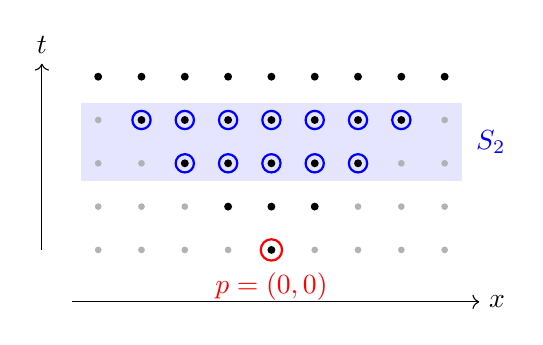
\begin{tikzpicture}[scale=0.55]
  \fill[Blue!10] (-4.4,1.6) rectangle (4.4,3.4);
  \foreach \t in {0,...,4} \foreach \x in {-4,...,4} {
    \pgfmathtruncatemacro{\ax}{abs(\x)}
    \ifnum\ax>\t \fill[gray!60] (\x,\t) circle (2.2pt);
    \else \fill[black] (\x,\t) circle (2.6pt); \fi }
  \foreach \x in {-2,...,2} \draw[Blue,thick] (\x,2) circle (6pt);
  \foreach \x in {-3,...,3} \draw[Blue,thick] (\x,3) circle (6pt);
  \draw[red,thick] (0,0) circle (7pt);
  \node[red,below] at (0,-0.3) {$p=(0,0)$};
  \draw[->] (-5.3,0) -- (-5.3,4.3) node[above] {$t$};
  \draw[->] (-4.6,-1.2) -- (4.8,-1.2) node[right] {$x$};
  \node[Blue,right] at (4.5,2.5) {$S_2$};
\end{tikzpicture}
\caption{The future of $p=(0,0)$ in the lattice $\Z^2$ (black points: $|x|\leq t$) and the
slices $S_2$ (shaded). The circled points form $J(\{p\})\cap S_2$.}
\label{fig:lattice}
\end{figure}

\noindent\motiv{The three relations among sets of lattice points are these. Inclusion
$O\subseteq O'$. Orthogonality: $O_1\perp O_2$ when no point of $O_1$ is comparable with a
point of $O_2$. Dependence: $O\dep O'$ when \revh{for every finite set $Y\subseteq O$} some pair of
slices meets the causal shadow of \revh{$Y$} only inside $O'$, that is, \revh{$J(Y)\cap S_{t_1}\subseteq O'$
for some $t_1$, which may depend on $Y$. Observables will be localized in finite sets, which is why
finite parts of $O$ suffice; for finite $O$ one takes $Y=O$.} For the point $p=(0,0)$:}
\begin{itemize}[leftmargin=2em]
\item \motiv{$\{p\}\perp\{(0,1)\}$ and $\{p\}\perp\{(1,2)\}$, since $|1|>0$ and $|2|>1$;
but $\{p\}$ and $\{(1,1)\}$ are not orthogonal, since $(1,1)$ lies on the future light cone of
$p$.}
\item \motiv{$J(\{p\})\cap S_2$ consists of the points $(2,x)$ with $|x|\leq2$ and $(3,x)$
with $|x|\leq3$ (Figure~\ref{fig:lattice}), so $\{p\}\dep O'$ for every $O'$ containing these
twelve points.}
\item \motiv{$\{p\}\dep\{p\}$ fails: for every $t_1$ the set $J(\{p\})\cap S_{t_1}$ contains at
least four points, \vet{so dependence is not reflexive.}}
\item \motiv{\revh{For the slice $O=\{(0,x):x\in\Z\}$ and $O'=\{(t,x):t\geq1,\ |x|\leq t^2\}$,
$O\dep O'$: a finite $Y\subseteq O$ lies in $|x|\leq R$, and $J(Y)\cap S_{t_1}$ lies in
$|x|\leq R+t_1+1\leq t_1^2$ for large $t_1$. No single pair of slices serves all of $O$, since
$J(O)$ is all of $\Z^2$.}}
\end{itemize}
\end{extra}

\dimockonly{\noindent\motiv{\revm{The regions of spacetime carry three relations that the axioms use: inclusion, orthogonality (spacelike separation) and dependence (one region determines another causally). The definition below keeps only the properties of these relations that the axioms need; Example~\ref{ex:gh-index} is the case of a globally hyperbolic spacetime.}}}


\begin{definition}[Causal index]\label{def:causal-index}
Let $(\cR,\leq)$ be a preordered set, whose elements are called regions. A \emph{causal index}
on $\cR$ consists of two relations, \emph{orthogonality} $O_1\perp O_2$ and \emph{dependence}
$O\dep O'$ (read: $O$ is causally dependent on $O'$), such that for all regions:
\begin{enumerate}[label=(\roman*),leftmargin=2.5em]
\item $O_1\perp O_2$ implies $O_2\perp O_1$;
\item $O_0\leq O_1$ and $O_1\perp O_2$ imply $O_0\perp O_2$;
\item $O_0\leq O$ and $O\dep O'$ imply $O_0\dep O'$;
\item $O\dep O'$ and $O'\leq O_1$ imply $O\dep O_1$.
\end{enumerate}
\end{definition}
From (i) and (ii), orthogonality is also antitone in its second argument: $O_3\leq O_2$ and
$O_1\perp O_2$ imply $O_1\perp O_3$.

\begin{extra}
\begin{example}[The lattice]\label{ex:lattice-index}
The subsets of $\Z^2$ ordered by inclusion, with $\perp$ and $\dep$ as above, form a causal
index. Condition~(i) holds because comparability is symmetric, and (ii) because, for
$O_0\subseteq O_1$, a comparable pair in $O_0\times O_2$ would lie in $O_1\times O_2$. For (iii), \revh{a finite subset of $O_0\subseteq O$ is a finite subset of $O$}. For (iv), enlarging $O'$
preserves the inclusion \revh{$J(Y)\cap S_{t_1}\subseteq O'$}.
\end{example}
\end{extra}

\begin{example}[A globally hyperbolic spacetime]\label{ex:gh-index}
On a globally hyperbolic Lorentzian manifold $(M,g)$ take as regions the open sets with
compact closure. Let $O_1\perp O_2$ when no causal curve joins a point of $O_1$ to a point of
$O_2$; this is \revb{the spacelike separation of~\cite{dimock}}. Let $O\dep O'$ when there is a \revc{smooth spacelike} Cauchy surface
$\Sigma$ such that every endless causal curve through a point of $O$ meets $\Sigma$ in $O'$;
this is the form of causal dependence used in the proof of \revb{Theorem~4 of~\cite[p.~226]{dimock}}.
Conditions (i)--(iv) hold because a causal curve traversed backwards is causal, a curve
through $O_0\subseteq O$ passes through $O$, and a curve meeting $\Sigma$ in $O'$ meets it in
every region containing $O'$.
\end{example}

\begin{remark}[\revm{Dependence through curves}]\label{rem:dimock-dep}
\vet{\revb{The other formulation of~\cite{dimock}}, every endless causal curve through $O$ meets
$O'$~\cite[p.~220]{dimock}, satisfies (i)--(iv) for the same reasons.}
\end{remark}

\begin{extra}
\noindent\motiv{\vet{In the lattice, comparability replaces causal curves and a pair of slices
replaces a Cauchy surface}\revi{, chosen for each finite part of $O$ (Remark~\ref{rem:green-dep-spacetime}
compares the two forms)}\vet{.}}
\end{extra}

\begin{definition}[Isomorphism of causal indices]\label{def:iso}
An \emph{isomorphism} from a causal index on $\cR$ to a causal index on $\cR'$ is a bijection
$\kappa:\cR\to\cR'$ such that $\kappa O\leq\kappa O'\iff O\leq O'$,
$\kappa O_1\perp\kappa O_2\iff O_1\perp O_2$ and $\kappa O\dep\kappa O'\iff O\dep O'$ for all
regions. The isomorphisms of a causal index to itself form a group $\Aut$ under composition,
$(\kappa_1\kappa_2)(O)=\kappa_1(\kappa_2O)$, with the identity as unit.
\end{definition}
Identities, composites and inverses of isomorphisms are isomorphisms, by inspection of the
three equivalences.

\begin{extra}
\begin{example}[Symmetries of the lattice]\label{ex:lattice-aut}
Each point map below sends regions to regions, and the induced map on subsets of $\Z^2$ is an
automorphism of the causal index of Example~\ref{ex:lattice-index}.
\begin{itemize}[leftmargin=2em]
\item A translation $(t,x)\mapsto(t+a,x+b)$ preserves the order of points, hence $J$ and
$\perp$, and maps $S_{t_1}$ to $S_{t_1+a}$.
\item The reflection $(t,x)\mapsto(t,-x)$ preserves the order of points and each slice.
\item The time reversal $(t,x)\mapsto(-t,x)$ reverses the order of points, so it preserves
comparability, $J$ and $\perp$, and maps $S_{t_1}$ to $S_{-t_1-1}$.
\end{itemize}
Regions are ordered by inclusion, which all three maps preserve. \revi{Each map is a bijection of
$\Z^2$ that sends finite sets to finite sets and pairs of slices to pairs of slices, with
$J(\kappa Y)=\kappa J(Y)$, and its inverse is of the same kind, so $\dep$ is preserved in both
directions.}
\end{example}
\end{extra}

\begin{remark}[Time orientation]\label{rem:time-orientation}
\vet{\revo{A time reversal, where the spacetime has one (\extraonly{the lattice of Example~\ref{ex:lattice-aut}, }Minkowski space),} is a symmetry of the causal index. It exchanges the retarded and advanced
propagators of the wave equation~\cite{bgp}, hence $E\mapsto-E$ and $\sigma\mapsto-\sigma$, and by
Remark~\ref{rem:antisymplectic} no $*$-isomorphism sends each Weyl operator $W(u)$ to its time
reverse. Covariance of the free field is therefore required only for maps that preserve the
time orientation.}\extraonly{ \revc{The argument excludes the map of test functions induced by a time
reversal, not every linear map over it: Remark~\ref{rem:massless-reversal} gives a symmetry of the
massless lattice field over the time reversal.}}
\end{remark}

\subsection{Nets and \revd{their axioms}}

\begin{definition}[Net]\label{def:net}
Let $A$ be a C*-algebra and $\cR$ a preordered set. A \emph{net} in $A$ over $\cR$ assigns to
each region $O$ a norm-closed $*$-subalgebra $\cA(O)$ of $A$, the \emph{local algebra} of $O$,
such that $O\leq O'$ implies $\cA(O)\subseteq\cA(O')$ (\emph{isotony}).
\end{definition}
\noindent Each local algebra, being norm closed, is itself a C*-algebra, and it contains the unit of
$A$.

\begin{remark}[The global algebra]\label{rem:global-algebra}
\vet{\revb{In~\cite{dimock} the global algebra is} the closure of the union of the local algebras; here
the net lives in a given algebra $A$, and the generation axiom below states that $A$ is \revo{the C*-algebra generated by the local algebras, which is} that
closure \revo{when the regions are directed (any two lie in a third)}.}
\end{remark}
\noindent\artefact{A net does not carry a causal index; each axiom takes one as an
argument, so that one net can be tested against several causal structures on the same
regions.}

\begin{definition}[The axioms]\label{def:axioms}
Let $\cA$ be a net in $A$ over a causal index on $\cR$.
\begin{enumerate}[label=(N\arabic*),leftmargin=3em]
\item $\cA$ is \emph{generating} if the C*-subalgebra generated by $\bigcup_O\cA(O)$ is $A$.
\item $\cA$ is \emph{causal} if $O_1\perp O_2$ implies $ab=ba$ for all $a\in\cA(O_1)$ and
$b\in\cA(O_2)$.
\item $\cA$ has the \emph{time-slice property} if $O\dep O'$ implies
$\cA(O)\subseteq\cA(O')$.
\end{enumerate}
A representation $\pi:A\to B(H)$ on a complex Hilbert space $H$ is \emph{irreducible} if every
bounded operator $T$ with $T\pi(a)=\pi(a)T$ for all $a\in A$ is a multiple of the identity.
The algebra $A$ is \emph{primitive} if it has an injective irreducible representation on a
nonzero Hilbert space.
\end{definition}
\artefact{The Hilbert spaces allowed in primitivity range over a fixed universe of Hilbert
spaces, determined by $A$. This is no restriction: if $\pi$ is irreducible and $\xi\neq0$, the closure of
$\pi(A)\xi$ is a nonzero closed subspace invariant under $\pi(A)$, and the projection onto it
commutes with $\pi(A)$, so it is the identity and $H=\overline{\pi(A)\xi}$. Hence $H$ has a dense subset indexed by
$A$, and $H$ is unitarily equivalent to a Hilbert space in the universe of $A$.}\par\medskip

\begin{remark}[Irreducibility]\label{rem:irreducible}
\vet{Irreducibility is defined here by a trivial commutant. For representations of C*-algebras
this is equivalent to the absence of closed invariant subspaces other than $0$ and
$H$\revb{ (see, e.g.,~\cite[Ch.~2]{bratteli-robinson-1})}: the commutant of $\pi(A)$ is a von Neumann algebra, so it equals $\C1$ exactly when its
only projections are $0$ and $1$, and its projections are the projections onto closed
invariant subspaces.}
\end{remark}

\begin{remark}[The time-slice axiom]\label{rem:time-slice}
\rev{\revb{Axiom~4 of~\cite[p.~220]{dimock}} reads: if $O$ is causally dependent on $O'$, then
$\cA(O)\subseteq\cA(O')$. \revm{This is (N3) when dependence is taken in the sense of the
spacetime; (N3) for a given causal index is called the time-slice property.} \revb{There} the meaning of causal dependence is left open,
naming as a strong form that every endless causal curve through $O$ meets $O'$
(Remark~\ref{rem:dimock-dep}); \revm{the proof of Theorem~4 of~\cite[p.~226]{dimock} uses}
the form of Example~\ref{ex:gh-index}\revi{; \extraonly{the lattice and }Green data use a pointwise form,
which the form of Example~\ref{ex:gh-index} implies (Remark~\ref{rem:green-dep-spacetime})\revjt{ for the
Green data of Remark~\ref{rem:green-continuum}, and for those of \revm{Chapters~\ref{sec:minkowski}
and~\ref{sec:mass}} when the Cauchy surface is flat (Remark~\ref{rem:mink-slabs})}}. The time-slice axiom of locally
covariant field theory, by which the algebra of a neighbourhood of a Cauchy surface is the
whole algebra, is a different statement\revm{; it is not assumed here}\revo{. For Green data, (N3) gives it for the slabs of the cutoffs, and, for the Green data of Remark~\ref{rem:green-continuum}, for neighbourhoods of every smooth spacelike Cauchy surface (after Theorem~\ref{thm:green-axioms})}.}
\end{remark}

\begin{table}[ht]
\centering\small
\begin{tabular}{@{}ll>{\raggedright\arraybackslash}p{0.36\textwidth}@{}}
\toprule
\revb{Axiom of~\cite[\S1]{dimock}} & content & here \revm{(defined; proved)} \\
\midrule
Axiom 1 & nets of local observables, $\cA=\overline{\bigcup_O\cA(O)}$ &
Definition~\ref{def:net} and (N1)\revm{; Theorems~\ref{thm:weyl-net}} \revo{(for Green data with Proposition~\ref{prop:green-phase}) and}\revm{ \ref{thm:kg-field}} \\
Axiom 2 & primitivity & Definition~\ref{def:axioms}\revf{; Theorem~\ref{thm:primitive}}\revm{, \ref{thm:dimock}} \\
Axiom 3 & first causality (spacelike commutativity) & (N2)\revm{; as for Axiom~1} \\
Axiom 4 & second causality (time slice) & (N3)\revm{; as for Axiom~1, over the causal index at hand} \\
Axiom 5 & covariance & Definition~\ref{def:covariance}\revm{; Theorems~\ref{thm:ccr-cov}, \extraonly{\ref{thm:lattice-net}, }\ref{thm:mink-covariance}, \ref{thm:kg-field}(c)} \\
\bottomrule
\end{tabular}
\caption{\revb{The axioms of~\cite{dimock}} and \revg{where they are defined or proved}.}
\label{tab:dimock}
\end{table}

\begin{definition}[Covariance]\label{def:covariance}
Let $\cA$ be a net in $A$ over a causal index on $\cR$, and $\cA'$ a net in $A'$ over a causal
index on $\cR'$. A pair $(\kappa,\alpha)$ of an isomorphism $\kappa$ of the causal indices and
a $*$-isomorphism $\alpha:A\to A'$ is a \emph{covariance pair} from $\cA$ to $\cA'$ if
\begin{equation}\label{eq:covariance}
\alpha\bigl(\cA(O)\bigr)=\cA'(\kappa O)\qquad\text{for every region }O.
\end{equation}
Two nets over the same causal index are \emph{isomorphic} if some $(\mathrm{id},\alpha)$ is a
covariance pair between them. A net $\cA$ is \emph{covariant under} a group $\Gamma$, given
group homomorphisms $\gamma\mapsto\kappa_\gamma$ into $\Aut$ and $\gamma\mapsto\alpha_\gamma$
into the $*$-automorphisms of $A$, if each $(\kappa_\gamma,\alpha_\gamma)$ is a covariance
pair from $\cA$ to itself.
\end{definition}

\begin{lemma}[Covariance pairs compose]\label{lem:pairs}
The pair $(\mathrm{id},\mathrm{id})$ is a covariance pair from a net to itself. If
$(\kappa_1,\alpha_1)$ is a covariance pair from $\cA$ to $\cA'$ and $(\kappa_2,\alpha_2)$ one
from $\cA'$ to $\cA''$, then $(\kappa_2\circ\kappa_1,\alpha_2\circ\alpha_1)$ is one from $\cA$
to $\cA''$, and $(\kappa_1^{-1},\alpha_1^{-1})$ is one from $\cA'$ to $\cA$.
\end{lemma}
\begin{proof}
The first claim is~\eqref{eq:covariance} for identities. For the second,
$\alpha_2\alpha_1(\cA(O))=\alpha_2(\cA'(\kappa_1O))=\cA''(\kappa_2\kappa_1O)$. For the third,
put $O=\kappa_1^{-1}O'$ in $\alpha_1(\cA(O))=\cA'(\kappa_1O)$ and apply $\alpha_1^{-1}$:
$\cA(\kappa_1^{-1}O')=\alpha_1^{-1}(\cA'(O'))$.
\end{proof}

\begin{remark}[Covariance as an assignment]\label{rem:axiom5}
\vet{\revb{Axiom~5 of~\cite{dimock}} asks for more than a single pair: an assignment
$\kappa\mapsto\alpha_\kappa$ on the isometries between spacetimes of one isometry class, with
$\alpha_{\mathrm{id}}=\mathrm{id}$ and $\alpha_{\kappa_1\kappa_2}=\alpha_{\kappa_1}
\alpha_{\kappa_2}$, each $(\kappa,\alpha_\kappa)$ a covariance pair. Such an assignment is a
construction on a family of nets. By Lemma~\ref{lem:pairs},
$(\kappa_1\kappa_2,\alpha_{\kappa_1}\alpha_{\kappa_2})$ is a covariance pair whenever the
factors are, so the composition law compares two covariance pairs over the same
isometry~$\kappa_1\kappa_2$.}
\end{remark}

\subsection{Nets generated by families of elements}

\noindent\motiv{The local algebras of the free field are generated by explicit unitaries, the
Weyl operators of test functions localized in the region. Whether two such algebras commute is
therefore a question about their generators. The answer needs one more hypothesis than the
commutation of the generators themselves\extraonly{ \vet{(Examples~\ref{ex:two-qubits}
and~\ref{ex:nilpotent})}}.}

\begin{extra}
\begin{example}[Two qubits]\label{ex:two-qubits}
In $A=M_2(\C)\otimes M_2(\C)$ let $s=\{\sigma_x\otimes1,\sigma_z\otimes1\}$ and
$s'=\{1\otimes\sigma_x,1\otimes\sigma_z\}$. Since
$\sigma_x\sigma_z=-\ii\sigma_y$, the $*$-algebra generated by $\sigma_x,\sigma_z$ contains
$1,\sigma_x,\sigma_y,\sigma_z$, which span $M_2(\C)$. Hence $\calg(s)=M_2(\C)\otimes1$ and
$\calg(s')=1\otimes M_2(\C)$, and every element of the first commutes with every element of the
second.
\end{example}
\end{extra}

\begin{extra}
\begin{example}[An element commuting with itself]\label{ex:nilpotent}
In $A=M_2(\C)$ let $e=\begin{psmallmatrix}0&1\\0&0\end{psmallmatrix}$ and $s=s'=\{e\}$. Every
element of $s$ commutes with every element of $s'$. But $ee^*=\begin{psmallmatrix}1&0\\0&0
\end{psmallmatrix}$ and $e^*e=\begin{psmallmatrix}0&0\\0&1\end{psmallmatrix}$, so $e$ does not
commute with $e^*$, and $\calg(s)$, which contains $e$ and $e^*$, is all of $M_2(\C)$ and is not
commutative. The generated algebras do not commute.
\end{example}
\end{extra}

\noindent\motiv{\extraonly{\vet{Commutation with adjoints is the hypothesis that
Example~\ref{ex:nilpotent} lacks.} }For a subset \revi{$s$} of $A$ let
\[
Z(\revi{s})=\{x\in A:\ xb=bx\ \text{and}\ xb^*=b^*x\ \text{for all }b\in \revi{s}\},
\]
the elements commuting with every element of \revi{$s$} and with its adjoint.}

\begin{lemma}[Commutation of generated algebras]\label{lem:commute}
Let \revk{$A$ be a C*-algebra and} $s,s'\subseteq A$, and suppose that every $a\in s$ commutes with every $b\in s'$ and with
every $b^*$, $b\in s'$. Then every element of $\calg(s)$ commutes with every element of
$\calg(s')$.
\end{lemma}
\begin{proof}
The set \revi{$Z(s)$} is a C*-subalgebra of $A$ for every \revi{$s$}. It is a unital subalgebra. It is closed
under the adjoint: taking adjoints in $xb=bx$ and $xb^*=b^*x$ gives $b^*x^*=x^*b^*$ and
$bx^*=x^*b$. It is norm closed, since each equation $xb=bx$ survives norm limits.

The hypothesis says $s\subseteq Z(s')$, so $\calg(s)\subseteq Z(s')$. Fix $x\in\calg(s)$. Both
$x$ and $x^*$ lie in $\calg(s)\subseteq Z(s')$, so every $b\in s'$ commutes with $x$ and with
$x^*$; that is, $s'\subseteq Z(\{x\})$. Hence $\calg(s')\subseteq Z(\{x\})$, and every element of
$\calg(s')$ commutes with $x$.
\end{proof}
\extraonly{In Example~\ref{ex:two-qubits} every generator is self-adjoint, so the hypothesis reduces to
commutation of the generators. In Example~\ref{ex:nilpotent} it fails, because $e$ does not
commute with $e^*$.}

\begin{definition}[Generated net]\label{def:generated}
A \emph{family of generators} in $A$ over $\cR$ assigns to each region $O$ a subset $G(O)$ of
$A$, with $G(O)\subseteq G(O')$ whenever $O\leq O'$. The net \emph{generated} by $G$ is
$\cA_G(O)=\calg(G(O))$.
\end{definition}
It is a net: each $\calg(G(O))$ is a norm-closed $*$-subalgebra, and $s_0\subseteq s_1$ implies
$\calg(s_0)\subseteq\calg(s_1)$.

\begin{proposition}[Axioms from generators]\label{prop:generated}
Let $G$ be a family of generators in \revk{a C*-algebra} $A$ over a causal index on \revk{a
preordered set} $\cR$ \revk{of regions}.
\begin{enumerate}[label=(\alph*),leftmargin=2.5em]
\item If, whenever $O_1\perp O_2$, every $a\in G(O_1)$ commutes with every $b\in G(O_2)$ and
with every $b^*$, $b\in G(O_2)$, then $\cA_G$ is causal.
\item If\revf{, whenever} $O\dep O'$\revf{,} $G(O)\subseteq\cA_G(O')$, then $\cA_G$ has the time-slice
property.
\item If $\calg\bigl(\bigcup_OG(O)\bigr)=A$, then $\cA_G$ is generating.
\item Let $G'$ be a family of generators in $A'$ over a causal index on $\cR'$, $\kappa$ an
isomorphism of the causal indices and $\alpha:A\to A'$ a $*$-isomorphism with
$\alpha(G(O))=G'(\kappa O)$ for every $O$. Then $(\kappa,\alpha)$ is a covariance pair from
$\cA_G$ to $\cA_{G'}$.
\end{enumerate}
\end{proposition}
\begin{proof}
\begin{enumerate}[leftmargin=2.5em]
\item[(a)] Lemma~\ref{lem:commute} with $s=G(O_1)$ and $s'=G(O_2)$.
\item[(b)] $\cA_G(O')$ is a C*-subalgebra containing $G(O)$, hence it contains $\calg(G(O))$.
\item[(c)] The C*-subalgebra generated by $\bigcup_O\cA_G(O)$ contains $\bigcup_OG(O)$, hence
contains $\calg(\bigcup_OG(O))=A$.
\item[(d)] A $*$-homomorphism maps the $*$-algebra generated by a set onto the $*$-algebra generated
by its image, so $\alpha(\alg(G(O)))=\alg(G'(\kappa O))$. It remains to pass to closures. A
$*$-homomorphism $\varphi$ between C*-algebras does not increase norms: the spectrum of
$\varphi(b)$ is contained in that of $b$, the norm of a self-adjoint element is its spectral
radius, and so $\|\varphi(a)\|^2=\|\varphi(a^*a)\|\leq\|a^*a\|=\|a\|^2$. Applied to $\alpha$ and
$\alpha^{-1}$, this makes $\alpha$ a homeomorphism, which maps the closure of a set onto the
closure of its image. Hence $\alpha(\calg(G(O)))=\calg(G'(\kappa O))$.
\end{enumerate}
\end{proof}

\begin{remark}[\revm{Moving generators}]\label{rem:weak-time-slice}
In (b) the generators of $O$ are required to lie in the closed algebra of $O'$, not in $G(O')$.
\rev{For the free field the Weyl operators are labelled by the classes $[f]$ of test
functions modulo the kernel of $E$ (Remark~\ref{rem:dictionary}), and the stronger inclusion
holds: if $O\dep O'$, every $f$ localized in $O$ has an $f'$ localized in $O'$ with $Ef'=Ef$\extraonly{ (on
the lattice this is Corollary~\ref{cor:lattice-dep})}, so $[f]=[f']$ and the generator
$W([f])$ of $O$ is a generator of $O'$. This is the step of the proof of \revb{Theorem~4
of~\cite[p.~226]{dimock}} that gives time slice. \revd{The classes and the net are constructed in Chapter~\ref{sec:phasespace}
(\extraonly{Example~\ref{ex:lattice-phase} and }Definition~\ref{def:weyl-net}).}}
\end{remark}

\clearpage
\section{The Weyl algebra}\label{sec:weyl}

\noindent\motiv{\vet{The observables of the free field are generated by the Weyl operators
$W(u)$, formally $e^{\ii\phi(u)}$, labelled by the vectors $u$ of a real vector space $V$ with an
alternating form $\sigma$, the classical phase space of the field. On the Hilbert space
$\ell^2(V)$ these operators are unitary, and the C*-algebra they generate serves as the algebra
$A$ of the axioms for the free field.} \revc{The Hilbert space $\ell^2(V)$ carries the regular
representation of the additive group $V$, twisted by the phases of $\sigma$. It serves to show that
Weyl operators exist; it is not the vacuum (Fock) representation of the field, which these notes do
not construct (Remarks~\ref{rem:separating} \revd{and~\ref{rem:fock}}).}}

\begin{remark}[Signs]\label{rem:dictionary}
\vet{Spacetime signature is mostly plus, and the Klein--Gordon operator is $P=-\square+m^2$
(\rev{$=\partial_t^2-\nabla^2+m^2$} in flat space). The \revd{causal propagator} is
$E=E^{\mathrm{adv}}-E^{\mathrm{ret}}$ for this $P$, so that
\rev{$[\phi(f),\phi(g)]=\ii\langle f,Eg\rangle$} and, at equal times, $[\phi(t,x),\Pi(t,y)]=\ii\delta(x-y)$ for the momentum $\Pi=\partial_t\phi$.\extraonly{ \rev{On the lattice this sign is
Proposition~\ref{prop:commutator}(e).}}
With $[f]$ the class of a test function $f$ modulo the kernel of $E$,
\rev{$\sigma([f],[g])=\langle f,Eg\rangle$} and $W(u)=e^{\ii\phi(u)}$, the Baker--Campbell--Hausdorff formula
$e^{X}e^{Y}=e^{X+Y}e^{[X,Y]/2}$ for a central commutator gives
$W(u)W(w)=e^{-\ii\sigma(u,w)/2}W(u+w)$, which is Proposition~\ref{prop:weyl-relation} below.}
\end{remark}

\subsection{Weyl operators on \texorpdfstring{$\ell^2(V)$}{\textell\texttwosuperior(V)}}

\noindent Throughout, $V$ is a real vector space of any dimension, which we regard as a discrete
set, and $\sigma$ is a real bilinear form on $V$ that is \emph{alternating}: $\sigma(u,u)=0$,
hence $\sigma(w,u)=-\sigma(u,w)$. $\sigma$ may be degenerate. $\ell^2(V)$ is the Hilbert space
of square-summable $\psi:V\to\C$, and $\delta_v$ is the indicator function of $\{v\}$.

\begin{definition}[Weyl operator]\label{def:weyl}
For $u\in V$, $(W(u)\psi)(v)=e^{\ii\sigma(u,v)/2}\,\psi(v+u)$.
\end{definition}

\begin{lemma}[Isometry]\label{lem:weyl-isometry}
\revk{The Weyl operators on $\ell^2(V)$ (Definition~\ref{def:weyl}) satisfy} $\|W(u)\psi\|=\|\psi\|$
for \revk{all $u\in V$,} $\psi\in\ell^2(V)$, and $W(0)=1$.
\end{lemma}
\begin{proof}
$|(W(u)\psi)(v)|^2=|\psi(v+u)|^2$, and $v\mapsto v+u$ is a bijection of $V$, so the two sums of
squares have the same terms.
\end{proof}

\begin{proposition}[Weyl relation]\label{prop:weyl-relation}
\revk{For a real vector space $V$ with alternating form $\sigma$, the Weyl operators on $\ell^2(V)$
satisfy} $W(u)W(w)=e^{-\ii\sigma(u,w)/2}\,W(u+w)$ \revk{for all $u,w\in V$}.
\end{proposition}
\begin{proof}
$(W(u)W(w)\psi)(v)=e^{\ii\sigma(u,v)/2}e^{\ii\sigma(w,v+u)/2}\psi(v+u+w)$ and
$(W(u+w)\psi)(v)=e^{\ii\sigma(u+w,v)/2}\psi(v+u+w)$; by bilinearity the exponents differ by
$\ii\sigma(w,u)/2=-\ii\sigma(u,w)/2$.
\end{proof}

\begin{proposition}[Unitarity]\label{prop:weyl-unitary}
\revk{For $u\in V$ the Weyl operator $W(u)$ on $\ell^2(V)$ satisfies} $W(u)W(-u)=1$, $W(u)^*=W(-u)$, and $W(u)$ is unitary.
\end{proposition}
\begin{proof}
Proposition~\ref{prop:weyl-relation} and $\sigma(u,u)=0$ give $W(u)W(-u)=W(0)=1$. An isometry
$a$ satisfies $a^*a=1$, by polarization of $\langle a\psi,a\psi\rangle=\langle\psi,\psi\rangle$.
Hence $W(u)^*=W(u)^*W(u)W(-u)=W(-u)$, and $W(u)W(u)^*=W(u)W(-u)=1$.
\end{proof}

\begin{definition}[CCR algebra]\label{def:ccr}
$\CCR(V,\sigma)=\calg\{W(u):u\in V\}$, the C*-subalgebra of the bounded operators on
$\ell^2(V)$ generated by the Weyl operators.
\end{definition}

\begin{example}[One degree of freedom]\label{ex:one-dof}
For $V=\R^2$ with $\sigma((a,b),(a',b'))=ab'-ba'$, the operators \revd{$W(a,0)$ and $W(0,b)$
satisfy $W(a,0)W(0,b)=e^{-\ii ab}W(0,b)W(a,0)$} by Proposition~\ref{prop:weyl-relation} applied twice.
This is the Weyl form $e^{\ii a\hat q}e^{\ii b\hat p}=e^{-\ii ab}e^{\ii b\hat p}e^{\ii a\hat q}$
of $[\hat q,\hat p]=\ii$. On $\ell^2(\R^2)$, however, \rev{$\lambda\mapsto W(\lambda u)$} is not continuous: for
\rev{$\lambda\neq0$} and $u\neq0$, \rev{$W(\lambda u)\delta_0=\delta_{-\lambda u}$} is orthogonal to $\delta_0$, so
\rev{$\|W(\lambda u)\delta_0-\delta_0\|=\sqrt2$}. The unitary group \rev{$\lambda\mapsto W(\lambda u)$} is therefore not
strongly continuous, \revd{so it has no self-adjoint generator, since $\lambda\mapsto e^{\ii\lambda A}$ is
strongly continuous for every self-adjoint $A$~\cite[Theorem~VIII.7]{reed-simon}}: no field operator
$\phi(u)$ exists in this representation.
\end{example}

\begin{example}[Zero form]\label{ex:sigma-zero}
For $\sigma=0$ the Weyl operators commute, $W(u)W(w)=W(u+w)$, and $\CCR(V,0)$ is commutative:
the closure of the commutative algebra spanned by the $W(u)$ is commutative.
\end{example}

\subsection{Weyl systems}

\begin{definition}[Weyl system]\label{def:weyl-system}
A \emph{Weyl system} over $(V,\sigma)$ is a unital C*-algebra $A$ with a map $W:V\to A$ such
that each $W(u)$ is unitary, $W(u)W(w)=e^{-\ii\sigma(u,w)/2}W(u+w)$, and
$\calg\{W(u):u\in V\}=A$.
\end{definition}

\begin{lemma}[Consequences of the relation]\label{lem:weyl-system}
In a Weyl system $W(0)=1$, $W(u)^*=W(-u)$ and $W(u)W(w)=e^{-\ii\sigma(u,w)}W(w)W(u)$; in
particular $W(u)$ and $W(w)$ commute when $\sigma(u,w)=0$.
\end{lemma}
\begin{proof}
The relation with $u=w=0$ gives $W(0)^2=W(0)$, and multiplying by $W(0)^*$ gives $W(0)=1$.
Then $W(u)W(-u)=e^{\ii\sigma(u,u)/2}W(0)=1$, so $W(-u)=W(u)^{-1}=W(u)^*$. Writing both
$W(u)W(w)$ and $W(w)W(u)$ as multiples of $W(u+w)$ gives the phase
$e^{-\ii\sigma(u,w)/2}/e^{-\ii\sigma(w,u)/2}=e^{-\ii\sigma(u,w)}$.
\end{proof}

\begin{proposition}[The concrete system]\label{prop:ccr-system}
$\CCR(V,\sigma)$ with the Weyl operators is a Weyl system.
\end{proposition}
\begin{proof}
Unitarity and the relation are Propositions~\ref{prop:weyl-unitary}
and~\ref{prop:weyl-relation}. For generation, the inclusion of $\CCR(V,\sigma)$ into the bounded
operators is an isometric $*$-homomorphism with closed image; it maps the $*$-subalgebra of
$\CCR(V,\sigma)$ generated by the $W(u)$ onto the one of the bounded operators generated by
them, so the closure of the former is the preimage of $\CCR(V,\sigma)$, which is all of it.
\end{proof}

\begin{remark}[\revm{Uniqueness and covariance}]\label{rem:weyl-covariance}
\vet{The zero algebra satisfies the three conditions of Definition~\ref{def:weyl-system};
$\CCR(V,\sigma)$ is not the zero algebra, since $\ell^2(V)\neq0$. Covariance is not part of the definition: for
$\CCR(V,\sigma)$ it is Proposition~\ref{prop:relabel}, and for another Weyl system we have to assume a family of
$*$-isomorphisms with $\alpha_L(W(u))=W'(Lu)$. \revm{For nondegenerate $\sigma$
(Definition~\ref{def:nondegenerate}) and both algebras nonzero such a family exists by the uniqueness
theorem for the CCR algebra~\cite{slawny} (see also~\cite{manuceau}
and~\cite[Thm.~5.2.8]{bratteli-robinson}), which~\cite[p.~225]{dimock} uses by citation; these
notes do not prove it, and it is not formalized. For degenerate $\sigma$ it can fail:} for $\sigma=0$ and $V\neq0$, $A=\C$ with $W\equiv1$ is a Weyl system, and
$\CCR(V,0)$ is not isomorphic to it, since the vectors $W(u)\delta_0=\delta_{-u}$
(Proposition~\ref{prop:right-weyl}) show that $\CCR(V,0)$ is not one-dimensional.}
\end{remark}

\subsection{Relabelling}

\noindent Let $(V',\sigma')$ be a second space and $L:V\to V'$ a linear bijection that is
\emph{symplectic}: $\sigma'(Lu,Lv)=\sigma(u,v)$.

\begin{definition}[Relabelling unitary]\label{def:relabel}
$(U_L\psi)(v')=\psi(L^{-1}v')$ for $\psi\in\ell^2(V)$ and $v'\in V'$.
\end{definition}

\begin{proposition}[Relabelling]\label{prop:relabel}
\revk{Let $L:V\to V'$ be a linear bijection with $\sigma'(Lu,Lv)=\sigma(u,v)$ and $U_L$ its
relabelling unitary (Definition~\ref{def:relabel}). Then:}
\begin{enumerate}[label=(\alph*),leftmargin=2.5em]
\item $U_L:\ell^2(V)\to\ell^2(V')$ is unitary, $U_L^*=U_{L^{-1}}$, $U_{\mathrm{id}}=1$ and
$U_{L_2L_1}=U_{L_2}U_{L_1}$.
\item $U_LW(u)U_L^*=W'(Lu)$, where $W'$ are the Weyl operators of $(V',\sigma')$.
\item $\alpha_L(a)=U_LaU_L^*$ restricts to a $*$-isomorphism
$\alpha_L:\CCR(V,\sigma)\to\CCR(V',\sigma')$ with $\alpha_L(W(u))=W'(Lu)$,
$\alpha_{\mathrm{id}}=\mathrm{id}$ and $\alpha_{L_2L_1}=\alpha_{L_2}\alpha_{L_1}$.
\end{enumerate}
\end{proposition}
\begin{proof}
\begin{enumerate}[leftmargin=2.5em]
\item[(a)] $U_L$ reindexes along the bijection $L^{-1}$, so it preserves norms, and $U_{L^{-1}}$ is its
inverse; an invertible isometry is unitary. The composition law is
$\psi(L_1^{-1}L_2^{-1}v'')=\psi((L_2L_1)^{-1}v'')$.
\item[(b)] With $v=L^{-1}v'$,
$(U_LW(u)U_L^*\psi)(v')=e^{\ii\sigma(u,v)/2}\psi(L(v+u))=e^{\ii\sigma'(Lu,v')/2}\psi(v'+Lu)$.
\item[(c)] Conjugation by $U_L$ is a continuous $*$-isomorphism of the bounded operators. By (b) it
maps the Weyl operators of $V$ onto those of $V'$, hence the generated $*$-algebra into
$\CCR(V',\sigma')$, and by continuity its closure as well; the same holds for $L^{-1}$, which
gives the inverse. The identities follow from (a).
\end{enumerate}
\end{proof}

\begin{remark}[Time reversal]\label{rem:antisymplectic}
\vet{If $\sigma'(Lu,Lv)=-\sigma(u,v)$, as for time reversal, no $*$-homomorphism \revd{$\eta$} with
\revd{$\eta(W(u))=W'(Lu)$} \rev{into a nonzero algebra} exists unless $\sigma=0$: applying \revd{$\eta$} to
Proposition~\ref{prop:weyl-relation} gives $e^{-\ii\sigma(u,w)/2}=e^{\ii\sigma(u,w)/2}$, while
\rev{$\sigma(\lambda u,w)=\lambda\sigma(u,w)$} takes every real value when $\sigma(u,w)\neq0$. This is the
algebraic form of Remark~\ref{rem:time-orientation}.} \rev{The relation does not exclude an antilinear
map, which conjugates the phase, as in Wigner's treatment of time reversal\revb{~\cite[Ch.~26]{wigner}}; such a map is not a
$*$-homomorphism of complex algebras and lies outside Definition~\ref{def:covariance}.}
\end{remark}

\subsection{Right Weyl operators and the vector state}

\noindent\motiv{\rev{The operators and the state of this section are tools for \revf{Chapter~\ref{sec:simple}}. The right Weyl operators commute with the whole algebra and move
$\delta_0$ to every basis vector, which makes the vector state at $\delta_0$ faithful
(Remark~\ref{rem:separating}); and $\tau(W(v))=[v=0]$ picks out the coefficient of $1$ in a
finite linear combination of Weyl operators.}}

\begin{definition}[Right Weyl operator]\label{def:right-weyl}
$(R(w)\psi)(v)=e^{-\ii\sigma(w,v)/2}\,\psi(v+w)$, the Weyl operator of the form $-\sigma$.
\end{definition}

\begin{proposition}[Right operators]\label{prop:right-weyl}
\revk{For $w\in V$ the right Weyl operator $R(w)$ on $\ell^2(V)$ (Definition~\ref{def:right-weyl})}
is unitary, $R(w)^*=R(-w)$, $R(w)R(w')=e^{\ii\sigma(w,w')/2}R(w+w')$, and $R(w)$
commutes with every element of $\CCR(V,\sigma)$. Moreover $W(u)\delta_0=\delta_{-u}$ and
$R(w)\delta_0=\delta_{-w}$.
\end{proposition}
\begin{proof}
The first three claims are Propositions~\ref{prop:weyl-relation} and~\ref{prop:weyl-unitary}
for $-\sigma$. The exponents of $(W(u)R(w)\psi)(v)$ and $(R(w)W(u)\psi)(v)$ differ by
$-\ii(\sigma(w,u)+\sigma(u,w))/2=0$, so $R(w)$ commutes with every $W(u)$, and so does
$R(w)^*=R(-w)$. By Lemma~\ref{lem:commute}, with $s$ the set of Weyl operators and
$s'=\{R(w)\}$, $R(w)$ commutes with $\CCR(V,\sigma)$. Finally
$(W(u)\delta_0)(v)=e^{\ii\sigma(u,v)/2}[v+u=0]$, and at $v=-u$ the phase is
$e^{-\ii\sigma(u,u)/2}=1$; the same for $R(w)$.
\end{proof}

\begin{definition}[Vector state]\label{def:vector-state}
$\tau(a)=\langle\delta_0,a\,\delta_0\rangle$ for $a\in\CCR(V,\sigma)$.
\end{definition}

\begin{proposition}[Values of the vector state]\label{prop:vector-state}
\revk{The vector state $\tau$ of $\CCR(V,\sigma)$ (Definition~\ref{def:vector-state})} is linear, $\tau(1)=1$, $\tau(a^*a)=\|a\delta_0\|^2$, $|\tau(a)|\leq\|a\|$, and
$\tau(W(v))=1$ if $v=0$ and $0$ otherwise.
\end{proposition}
\begin{proof}
$\tau(a^*a)=\langle a\delta_0,a\delta_0\rangle$, and $|\tau(a)|\leq\|a\delta_0\|\leq\|a\|$ by
the Cauchy--Schwarz inequality. By Proposition~\ref{prop:right-weyl},
$\tau(W(v))=\langle\delta_0,\delta_{-v}\rangle$.
\end{proof}

\begin{remark}[The tracial state]\label{rem:tracial}
\revd{$\tau$ is \revf{a} \emph{tracial state} of the CCR algebra~\cite{petz}:
$\tau(W(u)W(w))=e^{-\ii\sigma(u,w)/2}[u+w=0]$ is symmetric in $u$ and $w$, since
$\sigma(u,-u)=0$, so $\tau(ab)=\tau(ba)$ by linearity and continuity. The vector $\delta_0$ is
cyclic, since $W(u)\delta_0=\delta_{-u}$, so $\ell^2(V)$ is the GNS representation of $\tau$. For
any dynamics the KMS condition at $\beta=0$ reduces to $\omega(ab)=\omega(ba)$, so tracial
states are the equilibrium states at infinite temperature~\cite[Remark~2]{derezinski-pillet};
$\tau$ is not a vacuum.} \revf{For nondegenerate $\sigma$ it is the only tracial state: a tracial
state $\omega$ has $\omega(W(v))=\omega(W(u)W(v)W(u)^*)=e^{-\ii\sigma(u,v)}\omega(W(v))$}
\revg{by Lemma~\ref{lem:weyl-system}; for $v\neq0$ nondegeneracy gives $w$ with $\sigma(w,v)\neq0$,
and a real multiple $u$ of $w$ has $\sigma(u,v)\notin2\pi\Z$, so $\omega(W(v))=0=\tau(W(v))$. By
linearity and continuity $\omega=\tau$.}
\end{remark}

\begin{remark}[Faithfulness and reducibility]\label{rem:separating}
\rev{If $a\in\CCR(V,\sigma)$ and $a\delta_0=0$, then $a=0$: for every $w$,
$a\delta_{-w}=aR(w)\delta_0=R(w)a\delta_0=0$ by Proposition~\ref{prop:right-weyl}, and a bounded
operator vanishing on the orthonormal basis $\{\delta_v\}$ is zero. Hence $\tau(a^*a)=\|a\delta_0\|^2$
vanishes only for $a=0$. For $V\neq0$ the representation on $\ell^2(V)$ is reducible: for
$w\neq0$, $R(w)$ commutes with $\CCR(V,\sigma)$ but is not a multiple of $1$, since
$R(w)\delta_0=\delta_{-w}$ is orthogonal to $\delta_0$. Primitivity therefore needs another
representation\revf{ (Remark~\ref{rem:irrep}); Lemma~\ref{lem:faithful} restates
the first claim}.}
\end{remark}

\begin{remark}[Fock representations]\label{rem:fock}
\revd{A Fock representation is the usual alternative to $\ell^2(V)$. It needs a complex
structure on $V$ compatible with $\sigma$, that is, a choice of vacuum, which a curved
spacetime does not single out~\cite[p.~219]{dimock}. For nondegenerate $\sigma$ its Weyl
operators generate a C*-algebra isomorphic to $\CCR(V,\sigma)$ by the uniqueness theorem of
Remark~\ref{rem:weyl-covariance}, so the net and its axioms are the same. It differs in two
ways. It is irreducible, and $\lambda\mapsto W(\lambda u)$ is strongly continuous, so field
operators exist by Stone's theorem. And a bounded symplectic map is implemented by a unitary
only when its antilinear part is Hilbert--Schmidt, by Shale's theorem~\cite{shale}, whereas on
$\ell^2(V)$ every symplectic bijection is (Proposition~\ref{prop:relabel}). \revf{Theorem~\ref{thm:primitive}
needs an irreducible representation, and a Fock representation is one
(Remark~\ref{rem:irrep}).}}
\end{remark}

\extraonly{\clearpage
\section{Propagators on the lattice}\label{sec:lattice}

\noindent\motiv{\vet{The Weyl operators of the free field are labelled by test functions,
two test functions giving the same operator when $E$ maps them to the same solution, and their
commutation relations are fixed by $E$, the difference of the advanced and retarded Green
operators (Remark~\ref{rem:dictionary}). On
the lattice $\Z^2$ both Green operators are given by an explicit kernel, and the two properties
of $E$ that the axioms need, vanishing at spacelike separation and a time-slice identity,
become statements about finitely many terms.}}

\subsection{The discrete Klein--Gordon equation}

\noindent Points of $\Z^2$ are $p=(t,x)$, ordered and compared as in
\revh{Chapter}~\ref{sec:nets}. A \emph{test function} is a finitely supported $f:\Z^2\to\R$; they form
a real vector space $\cD$. The operator $P$ below acts on all functions $h:\Z^2\to\R$, and a solution is an $h$ with
$Ph=0$. For $m^2\in\R$ (of either sign)
let
\[
(Ph)(t,x)=h(t+1,x)+h(t-1,x)-h(t,x+1)-h(t,x-1)+m^2h(t,x),\qquad
\langle f,h\rangle=\sum_pf(p)\,h(p).
\]
The operator $P$ is the discrete form of $-\square+m^2=\partial_t^2-\partial_x^2+m^2$, and it
maps $\cD$ into $\cD$.

\begin{lemma}[Symmetry of $P$]\label{lem:kg-symmetric}
\revk{The lattice Klein--Gordon operator $P$ satisfies} $\langle Pf,h\rangle=\langle f,Ph\rangle$ for
\revk{every test function} $f\in\cD$ and every $h\revk{:\Z^2\to\R}$.
\end{lemma}
\begin{proof}
Each term of $P$ is a translation or a multiple of the identity, and the substitution
$p\mapsto p-c$ in the finite sum $\sum_pf(p+c)h(p)$ moves a translation by $c$ from $f$ to a
translation by $-c$ on $h$. The translations occur in pairs $\pm c$ with equal coefficients.
\end{proof}

\begin{definition}[Retarded kernel]\label{def:kernel}
$K:\Z^2\to\R$ is given by $K(t,x)=0$ for $t\leq0$, $K(1,x)=[x=0]$, and, for $t\geq1$,
\[
K(t+1,x)=-K(t-1,x)+K(t,x+1)+K(t,x-1)-m^2K(t,x).
\]
\end{definition}

\begin{lemma}[The kernel]\label{lem:kernel}
\revk{The retarded kernel $K$ of Definition~\ref{def:kernel} satisfies:}
\begin{enumerate}[label=(\alph*),leftmargin=2.5em]
\item $PK=\delta_{(0,0)}$.
\item $K(t,x)\neq0$ implies $|x|\leq t-1$.
\item $K(t,-x)=K(t,x)$.
\item If $m^2=0$, then $K(t,x)\neq0$ implies that $t+x$ is odd.
\end{enumerate}
\end{lemma}
\begin{proof}
\begin{enumerate}[leftmargin=2.5em]
\item[(a)] For $t\geq1$, $(PK)(t,x)=0$ is the recursion. At $t=0$ only the term
$K(1,x)=[x=0]$ survives, and for $t\leq-1$ every term vanishes.
\end{enumerate}
\revm{Parts (b)--(d) follow by induction on $t\geq1$ over the pair of slices $t-1$, $t$, starting from
$K(0,\cdot)=0$ and $K(1,\cdot)$. The inductive steps:}
\begin{enumerate}[leftmargin=2.5em]
\item[(b)] each of the values $K(t-1,x)$, $K(t,x\pm1)$, $K(t,x)$ that
determine $K(t+1,x)$ vanishes unless $|x|\leq t$.
\item[(c)] $K(1,\cdot)$ and the recursion are invariant under
$x\mapsto-x$.
\item[(d)] for $m^2=0$, $K(t+1,x)$ is a sum of values at the points
$(t-1,x)$ and $(t,x\pm1)$, each with the parity of $t+1+x$, and $K(1,x)\neq0$ only at $x=0$.
\end{enumerate}
\end{proof}

\noindent\motiv{Part (b) says that $K$ lives strictly inside the forward light cone: a
signal moves at most one site per time step.}

\subsection{Green operators and the commutator function}

\begin{definition}[Green operators]\label{def:green}
For $f\in\cD$ and $p=(t,x)$,
\[
G^+f(p)=\sum_qf(q)\,K(p-q),\qquad G^-f(p)=\sum_qf(q)\,K(q_t-t,\,x-q_x),\qquad
Ef=G^-f-G^+f,
\]
where $q=(q_t,q_x)$. Thus \rev{$Ef(p)=\sum_qf(q)\Delta(p-q)$ with the \revd{commutator function}
$\Delta(t,x)=K(-t,x)-K(t,x)$}.
\end{definition}

\noindent\rev{The operator $G^+$ has support in the future of the source and is called
\emph{retarded}, as in physics; $G^-$ is \emph{advanced}, and $E=G^--G^+$ is advanced minus
retarded, as in Remark~\ref{rem:dictionary}. B\"ar, Ginoux and Pf\"affle name them the other way
round: their advanced Green operator $G_+$ is the one with support in the causal
future~\cite[Def.~3.4.1]{bgp}, and their $G=G_+-G_-$~\cite[\S3.4]{bgp} equals $-E$.} \revm{In~\cite[p.~222]{dimock}, $E=E^+-E^-$ with the support of $E^+f$ in
the causal future of $\supp f$, which is $-E$ here; the relation
$[\phi(f),\phi(f')]=\ii^{-1}\langle f,\revo{(E^+-E^-)}f'\rangle$ of~\cite[Thm.~2, p.~224]{dimock}\revo{, written with Dimock's $E^+-E^-=-E$,} agrees with
Remark~\ref{rem:dictionary}.}

\begin{lemma}[Uniqueness]\label{lem:unique}
If \revk{$h:\Z^2\to\R$ satisfies} $Ph=0$ \revk{for the lattice Klein--Gordon operator $P$} and $h$ vanishes at all times before some \rev{$t_0$}, or at all times after some \rev{$t_0$}, then
$h=0$.
\end{lemma}
\begin{proof}
$Ph=0$ expresses $h$ on the slice $t+1$ through the slices $t$ and $t-1$, and $h$ on the slice
$t-1$ through the slices $t$ and $t+1$. Induction in the respective direction gives $h=0$.
\end{proof}

\begin{proposition}[Green operators]\label{prop:green}
For \revk{every test function} $f\in\cD$\revk{, the Green operators $G^\pm$ of
Definition~\ref{def:green} satisfy}:
\begin{enumerate}[label=(\alph*),leftmargin=2.5em]
\item $PG^+f=PG^-f=f$;
\item $G^+f(p)\neq0$ implies $|x-q_x|\leq t-q_t-1$ for some $q\in\supp f$, and $G^-f(p)\neq0$
implies $|x-q_x|\leq q_t-t-1$ for some $q\in\supp f$;
\item $G^+Pf=G^-Pf=f$.
\end{enumerate}
\end{proposition}
\begin{proof}
\begin{enumerate}[leftmargin=2.5em]
\item[(a)] $P$ commutes with translations and with the finite sum, so
$PG^+f=\sum_qf(q)\delta_q=f$ by Lemma~\ref{lem:kernel}(a); the reflected kernel
$(t,x)\mapsto K(-t,x)$ also satisfies $P(\cdot)=\delta_{(0,0)}$, since $P$ is invariant under
$t\mapsto-t$.
\item[(b)] This is Lemma~\ref{lem:kernel}(b).
\item[(c)] $G^+Pf-f$ is annihilated by $P$ by (a) and vanishes at all times
before the support of $f$ by (b) \rev{(if $t_f$ is the earliest time of $\supp f$, then $Pf$ vanishes
before $t_f-1$, and the strict inequality in (b) makes $G^+Pf$ vanish before $t_f$)}, so it is zero by Lemma~\ref{lem:unique}; $G^-$ is the same
with the future.
\end{enumerate}
\end{proof}

\begin{proposition}[The commutator function]\label{prop:commutator}
For $f,g\in\cD$\revk{, the causal propagator $E$ and the commutator function $\Delta$ of
Definition~\ref{def:green} satisfy}:
\begin{enumerate}[label=(\alph*),leftmargin=2.5em]
\item $PEf=0$ and $EPf=0$;
\item \rev{$\Delta(-t,-x)=-\Delta(t,x)$}, hence $\langle f,Eg\rangle=-\langle g,Ef\rangle$;
\item if $\supp f\perp\supp g$, then $\langle f,Eg\rangle=0$;
\item if $m^2=0$, then \rev{$\Delta(t,x)=0$} whenever $t+x$ is even;
\item \rev{$\Delta(-1,x)=[x=0]$ and $\Delta(0,x)=0$}.
\end{enumerate}
\end{proposition}
\begin{proof}
\begin{enumerate}[leftmargin=2.5em]
\item[(a)] This is Proposition~\ref{prop:green}(a),(c).
\item[(b)] By Lemma~\ref{lem:kernel}(c), \rev{$\Delta(-t,-x)=K(t,x)-K(-t,x)=-\Delta(t,x)$}, and
\rev{$\langle f,Eg\rangle=\sum_{p,q}f(p)\Delta(p-q)g(q)$}.
\item[(c)] A nonzero \rev{$\Delta(p-q)$} forces $|x_p-x_q|\leq|t_p-t_q|-1$ by Lemma~\ref{lem:kernel}(b),
so $p$ and $q$ are comparable.
\item[(d)] This is Lemma~\ref{lem:kernel}(d) for both terms of \rev{$\Delta$}.
\item[(e)] \rev{$\Delta(-1,x)=K(1,x)$ and $\Delta(0,x)=K(0,x)-K(0,x)$}.
\end{enumerate}
\end{proof}

\noindent\motiv{\vet{Part (e) is the canonical commutation relation: with
$\sigma([f],[g])=\langle f,Eg\rangle$ as in Remark~\ref{rem:dictionary}, it gives
$[\phi(0,x),\phi(1,y)-\phi(0,y)]=\ii[x=y]$, the lattice form of $[\phi,\Pi]=\ii\delta$. The sign of $E$ is therefore the
one of canonical quantization.}}

\begin{example}[Opposite parity]\label{ex:lattice-witness}
For $m^2=0$, the recursion gives $K(2,\pm1)=1$, $K(2,0)=0$ and $K(3,0)=1$, so \rev{$\Delta(3,0)=-1$} and
$\langle\delta_{(0,0)},E\delta_{(3,0)}\rangle=\rev{\Delta(-3,0)}=1$. By
Proposition~\ref{prop:commutator}(d), a pair of points with a nonzero value of \rev{$\Delta$} at $m^2=0$
must have $t+x$ of opposite parity, as here.
\end{example}

\subsection{Time slice}

\begin{theorem}[Time slice]\label{thm:lattice-timeslice}
Let $f\in\cD$, $t_1\in\Z$, $h=Ef$, and let $\chi$ be the indicator of the times $t\geq t_1+1$.
Then $f'=P((1-\chi)h)$ is a test function with $\supp f'\subseteq S_{t_1}\cap J(\supp f)$ and
$Ef'=Ef$.
\end{theorem}
\begin{proof}
Since $Ph=0$, a term-by-term evaluation gives $f'(t_1,x)=-h(t_1+1,x)$,
$f'(t_1+1,x)=h(t_1,x)$, and $f'=0$ at all other times. If $f'(p)\neq0$, then $h(p')\neq0$ for
the other point $p'$ of $S_{t_1}$ with the same $x$, and Proposition~\ref{prop:green}(b) gives
$q\in\supp f$ with $|x-q_x|\leq|t_{p'}-q_t|-1\leq|t_p-q_t|$; so $p\in J(\supp f)$, a finite
set within $S_{t_1}$. Next, $G^+f'+\chi h$ is annihilated by $P$ and vanishes for $t\leq t_1$,
since $f'$ is supported at times $\geq t_1$; and $G^-f'-(1-\chi)h$ is annihilated by $P$ and
vanishes for $t\geq t_1+1$, since $f'$ is supported at times $\leq t_1+1$. By
Lemma~\ref{lem:unique} both vanish, and $Ef'=(1-\chi)h+\chi h=h$.
\end{proof}

\noindent\motiv{\vet{The value $f'(t_1,x)=-h(t_1+1,x)$ can be nonzero where $h(t_1,x)=0$;
that $p$ still lies in $J(\supp f)$ comes from the strict inequality in
Lemma~\ref{lem:kernel}(b).}}

\begin{remark}[Time slice from the Green operators alone]\label{rem:timeslice-direct}
\rev{Given the support statement, the identity $Ef'=Ef$ also follows from the identities
$PG^\pm f=f$ and $G^\pm Pf=f$ on test functions and the support bounds of
Proposition~\ref{prop:green}, without applying Lemma~\ref{lem:unique} to $\chi h$ and
$(1-\chi)h$; \revc{these notes prove the identities $G^\pm Pf=f$ with that lemma, but they also follow
from the formal adjointness $\langle g,G^+f\rangle=\langle G^-g,f\rangle$ for $f,g\in\cD$\revh{, with
the pairing $\sum_pf(p)h(p)$ written in either order when one argument is finitely supported}, a
consequence of Lemma~\ref{lem:kernel}(c): $\langle g,G^+Pf\rangle=\langle
G^-g,Pf\rangle=\langle PG^-g,f\rangle=\langle g,f\rangle$ by Lemma~\ref{lem:kg-symmetric} and
Proposition~\ref{prop:green}(a), and likewise for $G^-$.} The function \revd{$k$}$=(1-\chi)G^+f+\chi G^-f$ is a test
function: $G^+f$ vanishes before the earliest time of $\supp f$ and $G^-f$ after the latest, and
each time slice meets $J(\supp f)$ in finitely many points. Since $PG^\pm f=f$,
\[
f'=P\bigl((1-\chi)G^-f\bigr)-P\bigl((1-\chi)G^+f\bigr)=f-P(\chi G^-f)-P\bigl((1-\chi)G^+f\bigr)
=f-Pk,
\]
and $E(f-f')=EPk=0$ by Proposition~\ref{prop:commutator}(a).}
\end{remark}

\begin{corollary}[Dependence moves test functions]\label{cor:lattice-dep}
If $O\dep O'$ in the causal index of Example~\ref{ex:lattice-index} and $\supp f\subseteq O$,
there is $f'\in\cD$ with $\supp f'\subseteq O'$ and $Ef'=Ef$.
\end{corollary}
\begin{proof}
\revh{$\supp f$ is a finite subset of $O$, so there is} $t_1$ with \revh{$J(\supp f)\cap S_{t_1}\subseteq O'$};
apply Theorem~\ref{thm:lattice-timeslice}.
\end{proof}
}
\clearpage
\begingroup
% chapter 4 accepted by the user, 27 Sep 2026
\section{The net of a classical phase space}\label{sec:phasespace}

\noindent\motiv{\vet{The observables of the free field are Weyl operators labelled by the
elements of its classical phase space, and an observable belongs to a region when the source that
generates the phase-space element can be chosen inside that region. This \revh{chapter} states that
information for an arbitrary causal index and proves that the net generated by the Weyl
operators of localized sources satisfies generation, causality and time slice in every
Weyl system (isotony holds for every generated net), and covariance in the CCR algebra, with the composition law of Axiom~5
of~\cite{dimock}.}}

\subsection{Phase-space data}

\begin{definition}[Phase-space data]\label{def:phase-space}
Fix a causal index on a preordered set $\cR$ of regions. \emph{Phase-space data} consist of real
vector spaces $\cD$ (test functions) and $V$ (the phase space), a monotone map
$O\mapsto\cD(O)$ from regions to linear subspaces of $\cD$ such that every $f\in\cD$ lies in
some $\cD(O)$, an alternating bilinear form $\sigma$ on $V$, and a surjective linear map
$f\mapsto[f]$ from $\cD$ onto $V$, which assigns to each test function the element of the phase
space it generates, such that:
\begin{enumerate}[label=(P\arabic*),leftmargin=3em]
\item if $O_1\perp O_2$, $f\in\cD(O_1)$ and $g\in\cD(O_2)$, then $\sigma([f],[g])=0$;
\item if $O\dep O'$ and $f\in\cD(O)$, there is $f'\in\cD(O')$ with $[f']=[f]$.
\end{enumerate}
\end{definition}
\noindent\motiv{\vet{``Phase-space data'' is a term of these notes; the object of the
literature is a symplectic space of solutions together with the test functions localized in each
region~\cite{bgp}. We require $f\mapsto[f]$ only to be surjective, so $V$ may be a
quotient of $\cD$ or a space of solutions, and $\sigma$ may be degenerate: nothing in this
\revh{chapter} uses more, and \revf{Chapter~\ref{sec:simple} adds nondegeneracy
(Definition~\ref{def:nondegenerate}) as a hypothesis}.} \revc{For the free field,
$V$ with $\sigma$ is the covariant phase space of physics, and $\sigma([f],[g])=\langle
f,Eg\rangle$ is the Peierls bracket of the smeared fields $\phi(f)$ and
$\phi(g)$~\cite{peierls}, whose quantization is $[\phi(f),\phi(g)]=\ii\langle
f,Eg\rangle$ (Remark~\ref{rem:dictionary}).}}

\begin{extra}
\begin{example}[The lattice field]\label{ex:lattice-phase}
On the lattice causal index of Example~\ref{ex:lattice-index} take $\cD$ the finitely supported
$f:\Z^2\to\R$, $\cD(O)=\{f:\supp f\subseteq O\}$, $V=\cD/\ker E$ with $E$ the \revd{causal propagator} of
Definition~\ref{def:green}, $[f]$ the class of $f$, and $\sigma([f],[g])=\langle f,Eg\rangle$.
Every $f$ lies in $\cD(\supp f)$, since every subset of $\Z^2$ is a region.
The form is well defined and alternating by Proposition~\ref{prop:commutator}(b):
$\langle f,Eg\rangle=-\langle g,Ef\rangle$ vanishes when $Ef=0$ or $Eg=0$, and
$\langle f,Ef\rangle=0$. Condition (P1) is Proposition~\ref{prop:commutator}(c), since
orthogonality is antitone in both arguments, and (P2) is Corollary~\ref{cor:lattice-dep}, since
$Ef'=Ef$ means $[f']=[f]$. The form is nondegenerate: \revc{$\sigma([f],[\delta_p])=-\langle\delta_p,Ef\rangle=-(Ef)(p)$, so}
$\sigma([f],[\delta_p])=0$ for all $p$ gives $Ef=0$.
\end{example}
\end{extra}

\begin{definition}[Isomorphism of phase-space data]\label{def:phase-iso}
An \emph{isomorphism} $\theta=(\kappa,\kappa_*,L)$ from phase-space data
$(\cD,V,\sigma,[\cdot])$ to $(\cD',V',\sigma',[\cdot]')$ consists of an isomorphism $\kappa$ of
the causal indices (Definition~\ref{def:iso}), a linear bijection $\kappa_*:\cD\to\cD'$ and a
linear bijection $L:V\to V'$ with
\[
\kappa_*(\cD(O))=\cD'(\kappa O),\qquad [\kappa_*f]'=L[f],\qquad \sigma'(Lu,Lv)=\sigma(u,v).
\]
\end{definition}
\noindent\motiv{\vet{The last condition makes $L$ symplectic, as in \revh{Chapter}~\ref{sec:weyl}. It is
where the time orientation enters: a time reversal exchanges the retarded and advanced Green
operators (Remark~\ref{rem:time-orientation}), so the triple formed by it, the pushforward of
test functions and the induced map $L$ has $\sigma'(Lu,Lv)=-\sigma(u,v)$ and is not an isomorphism
when $\sigma\neq0$.}\extraonly{ \revc{Other linear maps over a time reversal are not excluded:
Remark~\ref{rem:massless-reversal} gives one that is an isomorphism.}}}

\begin{extra}
\begin{remark}[Time reversal of the massless lattice field]\label{rem:massless-reversal}
\revc{Let $m^2=0$ in Example~\ref{ex:lattice-phase}, let $r(t,x)=(-t,x)$ be the time reversal of
Example~\ref{ex:lattice-aut}, let $\varepsilon(t,x)=(-1)^{t+x}$, and put
$\kappa_*f=\varepsilon\cdot(f\circ r)$. Then $\kappa_*(\cD(O))=\cD(rO)$, and $\kappa_*\kappa_*f=f$.
Since $G^-$ is defined by the time-reflected kernel, $G^\pm(f\circ r)=(G^\mp f)\circ r$, hence
$E(f\circ r)=-(Ef)\circ r$. By Proposition~\ref{prop:commutator}(d), $\Delta(p-q)\neq0$ implies
$\varepsilon(p)\varepsilon(q)=-1$, hence $E(\varepsilon g)=-\varepsilon\,Eg$. Together,
$E\kappa_*f=\varepsilon\cdot((Ef)\circ r)$. So $\kappa_*$ maps $\ker E$ onto itself,
$L[f]=[\kappa_*f]$ is a well-defined linear bijection of $V$, and
\[
\sigma(L[f],L[g])=\langle\varepsilon\cdot(f\circ r),\varepsilon\cdot((Eg)\circ r)\rangle
=\langle f,Eg\rangle=\sigma([f],[g]).
\]
Thus $\theta=(r,\kappa_*,L)$ is an isomorphism of phase-space data with $\theta\theta=\mathrm{id}$,
and by Theorem~\ref{thm:ccr-cov} $(r,\alpha_\theta)$ is a covariance pair of the CCR net of the
massless lattice field with $\alpha_\theta^2=\mathrm{id}$, so the net is covariant under the group
$\{\mathrm{id},r\}$. For $m^2\neq0$ the
sign $\varepsilon$ no longer anticommutes with $E$ \revd{(the recursion gives $K(2,0)=-m^2$, so $\Delta(2,0)=m^2$ at a point with $t+x$ even, and
$E(\varepsilon\delta_{(0,0)})(2,0)=m^2\neq-m^2=-\varepsilon(2,0)\,(E\delta_{(0,0)})(2,0)$)}, and these notes do not decide whether another
isomorphism over the time reversal exists.}
\end{remark}
\end{extra}

\begin{lemma}[Identity and composite]\label{lem:phase-iso}
\revp{For phase-space data $(\cD,V,\sigma,[\cdot])$ the identity maps form an isomorphism from
these data to themselves. Let $\theta_1=(\kappa_1,\kappa_{1*},L_1)$ be an isomorphism from
$(\cD,V,\sigma,[\cdot])$ to $(\cD',V',\sigma',[\cdot]')$ and $\theta_2=(\kappa_2,\kappa_{2*},L_2)$
an isomorphism from $(\cD',V',\sigma',[\cdot]')$ to $(\cD'',V'',\sigma'',[\cdot]'')$. Then
$\theta_2\theta_1=(\kappa_2\kappa_1,\kappa_{2*}\kappa_{1*},L_2L_1)$ is an isomorphism from
$(\cD,V,\sigma,[\cdot])$ to $(\cD'',V'',\sigma'',[\cdot]'')$.}
\end{lemma}
\begin{proof}
$\kappa_{2*}\kappa_{1*}(\cD(O))=\kappa_{2*}(\cD'(\kappa_1O))=\cD''(\kappa_2\kappa_1O)$;
$[\kappa_{2*}\kappa_{1*}f]''=L_2[\kappa_{1*}f]'=L_2L_1[f]$; and
$\sigma''(L_2L_1u,L_2L_1v)=\sigma'(L_1u,L_1v)=\sigma(u,v)$.
\end{proof}

\subsection{The net of a Weyl system}

\noindent\vet{From here on we fix phase-space data $(\cD,V,\sigma,[\cdot])$ on a causal index;
primed data $(\cD',V',\sigma',[\cdot]')$ denote a second such choice\revc{, possibly on another
causal index}.}

\begin{definition}[The net of a Weyl system]\label{def:weyl-net}
Let $(A,W)$ be a Weyl system over $(V,\sigma)$ (Definition~\ref{def:weyl-system}). Its generators
are $G(O)=\{W([f]):f\in\cD(O)\}$, a family of generators in the sense of
Definition~\ref{def:generated}, and its \emph{net} is the net they generate,
$\cA_W(O)=\calg\,G(O)$.
\end{definition}

\begin{theorem}[Generation, causality, time slice]\label{thm:weyl-net}
For \revk{phase-space data $(\cD,V,\sigma,[\cdot])$ on a causal index and} every Weyl system $(A,W)$
over $(V,\sigma)$\revk{,} the net $\cA_W$ is generating, causal and has the time-slice property.
\end{theorem}
\begin{proof}
The three properties follow from Proposition~\ref{prop:generated} once we check the
generators. Generation: $\bigcup_OG(O)=W(V)$, since every $u\in V$ is some $[f]$ and every $f$ lies
in some $\cD(O)$; and $W(V)$ generates $A$. Causality: for $O_1\perp O_2$, $f\in\cD(O_1)$,
$g\in\cD(O_2)$, (P1) gives $\sigma([f],[g])=0$, so $W[f]$ and $W[g]$ commute by
Lemma~\ref{lem:weyl-system}; the adjoint $W[g]^*=W[-g]$ is again a generator of $O_2$, so the
same argument applies to it. Time slice: for $O\dep O'$ and $f\in\cD(O)$, (P2) gives
$f'\in\cD(O')$ with $W[f]=W[f']\in G(O')$.
\end{proof}

\begin{extra}
\noindent\motiv{\vet{For the lattice field of Example~\ref{ex:lattice-phase} and the CCR algebra
this \revm{gives generation, causality and time slice} without
assumptions on the spacetime; \reve{Chapter~\ref{sec:latticenet} completes that instance with
translation covariance}.}}
\end{extra}

\subsection{Covariance}

\begin{theorem}[Covariance pairs from Weyl systems]\label{thm:weyl-cov}
Let $\theta=(\kappa,\kappa_*,L)$ be an isomorphism of phase-space data, $(A,W)$ and $(A',W')$ Weyl
systems over $(V,\sigma)$ and $(V',\sigma')$, and $\alpha:A\to A'$ a $*$-isomorphism with
$\alpha(W(u))=W'(Lu)$ for all $u$. Then $(\kappa,\alpha)$ is a covariance pair from $\cA_W$ to
$\cA'_{W'}$.
\end{theorem}
\begin{proof}
By Proposition~\ref{prop:generated}(d) it suffices that $\alpha(G(O))=G'(\kappa O)$, and
$\alpha(G(O))=\{W'(L[f]):f\in\cD(O)\}=\{W'([\kappa_*f]'):f\in\cD(O)\}=\{W'([f']'):f'\in
\cD'(\kappa O)\}$.
\end{proof}
\noindent\motiv{\vet{Only the first two conditions of Definition~\ref{def:phase-iso} enter
here, since $\alpha$ is given; \revc{the symplectic condition is preserved under composition
(Lemma~\ref{lem:phase-iso}) and is used in Theorem~\ref{thm:ccr-cov}, where it makes
$\alpha_\theta$ exist. When $A'\neq0$ it also follows from the hypotheses: applying $\alpha$ to
the Weyl relation gives $e^{-\ii\sigma(u,w)/2}=e^{-\ii\sigma'(Lu,Lw)/2}$, and the scaling argument
of Remark~\ref{rem:antisymplectic} gives $\sigma'(Lu,Lw)=\sigma(u,w)$.}}}

\begin{corollary}[Isomorphic Weyl systems]\label{cor:weyl-iso}
If $(A,W)$ and $(A',W')$ are Weyl systems over $(V,\sigma)$, both nets formed from the same
phase-space data, and $\alpha:A\to A'$ is a
$*$-isomorphism with $\alpha\circ W=W'$, the nets $\cA_W$ and $\cA'_{W'}$ are isomorphic.
\end{corollary}
\begin{proof}
Theorem~\ref{thm:weyl-cov} with the identity isomorphism.
\end{proof}
\noindent\motiv{\vet{For nondegenerate $\sigma$ and nonzero algebras such an $\alpha$ always
exists, by the uniqueness theorem for the CCR algebra~\cite{slawny} (see also~\cite{manuceau}); the paper
\cite[p.~225]{dimock} uses it, by citation, for the independence of the net from the
representation in its Theorem~3. These notes do not prove it and do not formalize it here; the
corollary carries $\alpha$ as a hypothesis.}}

\begin{definition}[The CCR net]\label{def:ccr-net}
The \emph{CCR net} of phase-space data is $\cA_W$ for the Weyl system $(\CCR(V,\sigma),W)$ of
Proposition~\ref{prop:ccr-system}. For an isomorphism $\theta=(\kappa,\kappa_*,L)$ let
$\alpha_\theta:\CCR(V,\sigma)\to\CCR(V',\sigma')$ be conjugation by the relabelling unitary $U_L$
(Proposition~\ref{prop:relabel}).
\end{definition}

\begin{theorem}[Covariance of the CCR net]\label{thm:ccr-cov}
For every isomorphism $\theta\revk{=(\kappa,\kappa_*,L)}$ \revk{from} phase-space data
\revk{$(\cD,V,\sigma,[\cdot])$ to $(\cD',V',\sigma',[\cdot]')$}, $(\kappa,\alpha_\theta)$ is a covariance
pair \revk{from the CCR net of the first to that of the second}, $\alpha_{\mathrm{id}}=\mathrm{id}$, and
$\alpha_{\theta_2\theta_1}=\alpha_{\theta_2}\alpha_{\theta_1}$.
\end{theorem}
\begin{proof}
Proposition~\ref{prop:relabel} gives $\alpha_\theta(W(u))=W'(Lu)$, $\alpha_{\mathrm{id}}=\mathrm{id}$
and $\alpha_{L_2L_1}=\alpha_{L_2}\alpha_{L_1}$, and the symplectic map of $\theta_2\theta_1$ is
$L_2L_1$ (Lemma~\ref{lem:phase-iso}). Theorem~\ref{thm:weyl-cov} gives the covariance pair.
\end{proof}
\noindent\motiv{\vet{This is Axiom~5 of~\cite[p.~220]{dimock} for the CCR net: an assignment
$\theta\mapsto\alpha_\theta$ with $\alpha_{\mathrm{id}}=\mathrm{id}$ and
$\alpha_{\theta_2\theta_1}=\alpha_{\theta_2}\alpha_{\theta_1}$, each $(\kappa,\alpha_\theta)$ a
covariance pair (Remark~\ref{rem:axiom5}), indexed by the isomorphisms of phase-space data. \revc{We obtain an assignment indexed by the isometries
themselves, as in~\cite{dimock}, by taking for each isometry the triple of the
induced map of regions, the pushforward of test functions and the induced map on $V$; pushforwards
compose, and $L$ is determined by $\kappa_*$ because $[\cdot]$ is surjective, so this choice
respects composition.}}}

\motiv{\vet{For the
free field these include the maps induced by the isometries that preserve the time orientation,
which commute with the Green operators by their uniqueness on a globally hyperbolic
spacetime~\cite[Cor.~3.4.3]{bgp}, a result \revk{formalized here only for the massless field on
Minkowski space (Theorem~\ref{thm:mink-unique}, Proposition~\ref{prop:mink-symmetry})} \revlt{and for
the Klein--Gordon field there (Theorem~\ref{thm:kg-field}(b), (c))}; the converse fails, since
$(\mathrm{id},-\mathrm{id},-\mathrm{id})$ is an isomorphism that no isometry induces \revc{when $\cD\neq0$}. Covariance under a group of
such isomorphisms is \revk{\extraonly{Theorem~\ref{thm:lattice-net} for the lattice translations and
}Theorem~\ref{thm:mink-covariance} \revlt{and Theorem~\ref{thm:kg-field}(c)} for the orthochronous Poincar\'e group}.}}
\endgroup

\extraonly{\clearpage
\begingroup
\section{The net of the lattice field}\label{sec:latticenet}

\noindent\motiv{\reve{This chapter restates Example~\ref{ex:lattice-phase} as numbered results,
including nondegeneracy, shows that no condition is vacuous, and constructs isomorphisms of phase-space data
for the lattice translations and the spatial reflection. With Chapter~\ref{sec:phasespace} this
gives the lattice CCR net with generation, causality, time slice and translation covariance, for
every $m^2$ and with no hypotheses. The last subsection shows that the net defined through Cauchy
data, as in~\cite[\S2]{dimock}, is the net of a pulled-back Weyl system, and for the
CCR algebra over Cauchy data is isomorphic to the lattice CCR net.}}

\medskip
\noindent\motiv{\reve{Throughout this chapter, $m^2\in\R$ is fixed, $\cD$ is the space of test functions on
$\Z^2$, and three consequences of Chapter~\ref{sec:lattice} are used repeatedly. By
Proposition~\ref{prop:commutator}(e), and for the third value by (b) with the evenness below,
\begin{equation}\label{eq:delta-slices}
\Delta(-1,x)=[x=0],\qquad \Delta(0,x)=0,\qquad \Delta(1,x)=-[x=0].
\end{equation}
By Lemma~\ref{lem:kernel}(b),(c), applied to each term of $\Delta(t,x)=K(-t,x)-K(t,x)$,
$\Delta(t,x)\neq0$ implies $|x|\leq|t|-1$, and $\Delta(t,-x)=\Delta(t,x)$. By
Proposition~\ref{prop:commutator}(a), $PEf=0$.}}

\subsection{Phase-space data}

\begin{proposition}[The lattice phase-space data]\label{prop:lattice-data}
\revlt{For $m^2\in\R$, the lattice test functions $\cD$ and the causal propagator $E$ of
Definition~\ref{def:green},} let $\cD(O)=\{f\in\cD:\supp f\subseteq O\}$, $V=\cD/\ker E$ with $[f]$ the class of $f$, and
$\sigma([f],[g])=\langle f,Eg\rangle$. Then $E$ is linear, $\sigma$ is a well-defined alternating
bilinear form, and $(\cD,V,\sigma,[\cdot])$ are phase-space data over the lattice causal index
(Example~\ref{ex:lattice-index}).
\end{proposition}
\begin{proof}
$(Ef)(p)=\sum_qf(q)\Delta(p-q)$ and $\langle f,h\rangle$ are finite sums, linear in $f$ and in $h$.
The form $(f,g)\mapsto\langle f,Eg\rangle$ vanishes when $Eg=0$, and when $Ef=0$ because
$\langle f,Eg\rangle=-\langle g,Ef\rangle$ (Proposition~\ref{prop:commutator}(b)); so it descends
to $V\times V$, and $\langle f,Ef\rangle=-\langle f,Ef\rangle$ makes it alternating. $\cD(O)$ is a
subspace, monotone in $O$, and $f\in\cD(\supp f)$. (P1) is Proposition~\ref{prop:commutator}(c),
since no point of a subset of $O_1$ is comparable with a point of a subset of $O_2$ when
$O_1\perp O_2$. (P2) is Corollary~\ref{cor:lattice-dep}: $Ef'=Ef$ means $f'-f\in\ker E$, that is,
$[f']=[f]$.
\end{proof}
\noindent\motiv{\reve{$V$ is taken as the quotient $\cD/\ker E$ rather than the space $E\cD$ of
solutions; the two are isomorphic through $[f]\mapsto Ef$.} \artefact{\reve{The quotient makes
$f\mapsto[f]$ a quotient map, and the form descends by the universal property.}}}

\begin{proposition}[Nondegeneracy]\label{prop:lattice-nondeg}
\revk{For the lattice phase-space data of Proposition~\ref{prop:lattice-data},}
$\sigma([f],[\delta_p])=-(Ef)(p)$ for all $f\revk{\in\cD}$ and $p\revk{\in\Z^2}$. \reve{By definition of $V$}, $[f]=0$ if
and only if $Ef=0$, and $\sigma(u,w)=0$ for all $w$ implies $u=0$.
\end{proposition}
\begin{proof}
$\sigma([f],[\delta_p])=-\langle\delta_p,Ef\rangle=-(Ef)(p)$. $[f]=0$ means $f\in\ker E$. If
$\sigma([f],w)=0$ for all $w$, then $(Ef)(p)=0$ for all $p$.
\end{proof}

\begin{example}[The conditions are not vacuous]\label{ex:lattice-nonvacuous}
(a) \reve{$\sigma\neq0$: the recursion gives $K(2,\pm1)=1$, $K(2,0)=-m^2$ and
$K(3,0)=-K(1,0)+K(2,1)+K(2,-1)-m^2K(2,0)=1+m^4$, so}
$\sigma([\delta_{(0,0)}],[\delta_{(3,0)}])=\Delta(-3,0)=-\Delta(3,0)=\reve{1+m^4}$\reve{, which is $1$ at
$m^2=0$} (Example~\ref{ex:lattice-witness}).
(b) The regions $\{(0,0)\}$ and $\{(0,1)\}$ are orthogonal, and $[\delta_{(0,0)}]$, $[\delta_{(0,1)}]$
are nonzero: by~\eqref{eq:delta-slices}, $\sigma([\delta_{(0,x)}],[\delta_{(1,x)}])=\Delta(-1,0)=1$.
(c) $O=\{(5,0)\}$ and $O'=J(O)\cap S_0$, of $11+9=20$ points, satisfy $O\dep O'$ and
$O\not\subseteq O'$, so the time-slice property is not isotony\reve{: the algebra of a point is
contained in that of a region, far from it in time, that does not contain the point}.
\end{example}

\subsection{Translations and the spatial reflection}

\noindent For $a\in\Z^2$ let $\kappa_a O=O+a$ and $(\kappa_{a*}f)(p)=f(p-a)$. Let
$\rho(t,x)=(t,-x)$, $\kappa_\rho O=\rho O$ and $(\kappa_{\rho*}f)(p)=f(\rho p)$.

\begin{lemma}[\revm{Covariance of $E$}]\label{lem:lattice-cov-E}
\revk{For $a\in\Z^2$ and the reflection $\rho(t,x)=(t,-x)$, the lattice causal propagator $E$
satisfies} $(E\kappa_{a*}f)(p)=(Ef)(p-a)$ and $(E\kappa_{\rho*}f)(p)=(Ef)(\rho p)$ \revk{for
$f\in\cD$}.
\end{lemma}
\begin{proof}
Substitute $q\mapsto q+a$, respectively $q\mapsto\rho q$, in $\sum_qf(q)\Delta(p-q)$; the second
uses $\Delta(\rho(p-q))=\Delta(p-q)$, the evenness of $\Delta$ in $x$.
\end{proof}

\begin{proposition}[Isomorphisms of the lattice data]\label{prop:lattice-iso}
\revm{For the lattice phase-space data of Proposition~\ref{prop:lattice-data}:}
\begin{enumerate}[label=(\alph*),leftmargin=2.5em]
\item For each $a\in\Z^2$, $\theta_a=(\kappa_a,\kappa_{a*},L_a)$ with \revk{$\kappa_aO=O+a$,
$\kappa_{a*}f=f(\cdot-a)$ and} $L_a[f]=[\kappa_{a*}f]$ is an
isomorphism \revm{of these data to themselves} (Definition~\ref{def:phase-iso}), and $L_0=\mathrm{id}$,
$L_{a+b}=L_aL_b$.
\item $\theta_\rho=(\kappa_\rho,\kappa_{\rho*},L_\rho)$ with \revk{$\kappa_\rho O=\rho O$,
$\kappa_{\rho*}f=f\circ\rho$ for the reflection $\rho(t,x)=(t,-x)$, and} $L_\rho[f]=[\kappa_{\rho*}f]$ is an
isomorphism \revm{of these data to themselves}.
\end{enumerate}
\end{proposition}
\begin{proof}
Both are cases of one construction: a bijection $\zeta$ of $\Z^2$ with
$\Delta(\zeta p-\zeta q)=\Delta(p-q)$ for all $p,q$, together with an automorphism $\kappa$ of the
causal index with $\kappa O=\zeta O$. \reve{Applying the hypothesis to $\zeta^{-1}p$ and $q$ gives
$E(f\circ\zeta^{-1})=(Ef)\circ\zeta^{-1}$, as in Lemma~\ref{lem:lattice-cov-E}.} So the pushforward
$f\mapsto f\circ\zeta^{-1}$, a linear bijection with $\cD(O)\mapsto\cD(\zeta O)$, maps $\ker E$
onto $\ker E$; $L[f]=[f\circ\zeta^{-1}]$ is a well-defined linear bijection, and $\langle
f\circ\zeta^{-1},E(g\circ\zeta^{-1})\rangle=\langle f,Eg\rangle$. For (a), $\zeta(p)=p+a$;
$L_0=\mathrm{id}$ and $L_{a+b}=L_aL_b$ because the pushforwards compose. For (b), $\zeta=\rho$
($\rho^{-1}=\rho$). In both cases $\kappa$ is an automorphism by
Example~\ref{ex:lattice-aut}\reve{, which lists the translations and the reflection}.
\end{proof}
\noindent\motiv{\reve{Example~\ref{ex:lattice-aut} lists the spatial reflection among the
automorphisms of the lattice causal index; what is new here is the isomorphism of phase-space data
over it. \revo{The time reversal $r$ carries one for $m^2=0$, with a sign twist (Remark~\ref{rem:massless-reversal}), and for $m^2\neq0$ these notes leave open whether it carries one;} the reflection carries
one for every $m^2$, without a sign twist.}}

\subsection{The net}

\begin{theorem}[The net of the lattice field]\label{thm:lattice-net}
For every $m^2\in\R$ the CCR net $\cA$ of the lattice phase-space data is generating, causal and
has the time-slice property, and it is covariant under the translation group $\Z^2$: with
$\alpha_a=\alpha_{\theta_a}$ (Definition~\ref{def:ccr-net}), $a\mapsto\kappa_a$ and $a\mapsto\alpha_a$
are group homomorphisms and every $(\kappa_a,\alpha_a)$ is a covariance pair.
\end{theorem}
\begin{proof}
Theorem~\ref{thm:weyl-net} for Proposition~\ref{prop:lattice-data} gives the first three
properties, and Theorem~\ref{thm:ccr-cov} with Proposition~\ref{prop:lattice-iso}(a) gives the
covariance pairs. $a\mapsto\kappa_a$ is a homomorphism since $O+0=O$ and $O+(a+b)=(O+b)+a$. The
$*$-isomorphism $\alpha_\theta$ depends on $\theta$ only through $L$, and $L_0=\mathrm{id}$,
$L_{a+b}=L_aL_b$, so Theorem~\ref{thm:ccr-cov} gives $\alpha_0=\mathrm{id}$ and
$\alpha_{a+b}=\alpha_a\alpha_b$.
\end{proof}
\noindent\motiv{\reve{The theorem has no hypotheses: the propagators are the explicit ones of
Chapter~\ref{sec:lattice}, and Example~\ref{ex:lattice-nonvacuous} shows that $\sigma\neq0$,
that orthogonal regions carry nonzero elements of $V$, and that dependence does not reduce to
inclusion. No hypothesis on $m^2$ is needed either: the axioms
say nothing about energy, so $m^2<0$, where the classical field grows exponentially, is included.
The theorem is the lattice form of Axioms 1, 3 and 4 of~\cite{dimock} and of the translation part
of Axiom~5; primitivity (Axiom~2) is \revf{Corollary~\ref{cor:lattice-dimock}, given an irreducible
representation}. By
Theorem~\ref{thm:ccr-cov} and Proposition~\ref{prop:lattice-iso}(b), $(\kappa_\rho,\alpha_{\theta_\rho})$
is a covariance pair as well.}}

\subsection{The Cauchy-data net}

\noindent\motiv{\reve{In~\cite[\S2, pp.~222--225]{dimock} the net is built from a
representation of the Weyl relations over Cauchy data: $e^{\ii\phi(f)}$ is represented by the Weyl
operator of the Cauchy data of $Ef$ on a Cauchy surface. On the lattice two consecutive time
slices play the part of a Cauchy surface (Chapter~\ref{sec:lattice}), and this subsection proves
that the net so defined is the net of a pulled-back Weyl system, isomorphic for the CCR algebra
to the net of Theorem~\ref{thm:lattice-net}.}}

\begin{definition}[Pullback of a Weyl system]\label{def:pullback}
Let $(V,\sigma)$ and $(V_S,\sigma_S)$ be real vector spaces with alternating forms, and
$\Lambda:V\to V_S$ a linear map with $\sigma_S(\Lambda u,\Lambda w)=\sigma(u,w)$. The
\emph{pullback} of a Weyl system $(A,W_S)$ over $(V_S,\sigma_S)$ along $\Lambda$ is the pair
$(A,W_S\circ\Lambda)$\reve{; it is a Weyl system when $\Lambda$ is onto (Proposition~\ref{prop:pullback})}.
\end{definition}

\begin{proposition}[Pullback]\label{prop:pullback}
\revk{Let $\Lambda:V\to V_S$ and $(A,W_S)$ be as in Definition~\ref{def:pullback}. Then}
$W_S\circ\Lambda$ consists of unitaries and satisfies the Weyl relation over $(V,\sigma)$. If
$\Lambda$ is onto, $(A,W_S\circ\Lambda)$ is a Weyl system over $(V,\sigma)$, and for phase-space
data with phase space $(V,\sigma)$ its net is $O\mapsto\calg\{W_S(\Lambda[f]):f\in\cD(O)\}$.
\end{proposition}
\begin{proof}
$W_S(\Lambda u)W_S(\Lambda w)=e^{-\ii\sigma_S(\Lambda u,\Lambda w)/2}W_S(\Lambda u+\Lambda w)
=e^{-\ii\sigma(u,w)/2}W_S(\Lambda(u+w))$. If $\Lambda$ is onto, the ranges of $W_S\circ\Lambda$
and $W_S$ coincide, so they generate $A$. The net is Definition~\ref{def:weyl-net}.
\end{proof}
\noindent\motiv{\reve{The relabelling of Proposition~\ref{prop:relabel} acts along symplectic
bijections and changes the algebra; the pullback keeps the algebra $A$ of $W_S$.}}

\begin{definition}[Cauchy data and the Cauchy map]\label{def:cauchy-map}
\emph{Cauchy data} are pairs $d=(d_0,d_1)$ of finitely supported functions $\Z\to\R$; they form a
real vector space $V_S$ with the \emph{Wronskian}
$\sigma_S(d,d')=\sum_x\bigl(d_0(x)d_1'(x)-d_1(x)d_0'(x)\bigr)$, an alternating form. For
$t_1\in\Z$ the \emph{Cauchy map} is
$\Lambda_{t_1}[f]=\bigl((Ef)(t_1,\cdot),\,(Ef)(t_1+1,\cdot)\bigr)$.
\end{definition}
\noindent $\Lambda_{t_1}$ is well defined and linear: $(Ef)(t,x)\neq0$ requires some $q\in\supp f$
with $|x-x_q|\leq|t-t_q|-1$, so each slice of $Ef$ is finitely supported, and $Ef$ depends only on
$[f]$. \reve{The data are the field on two consecutive slices. With the discrete momentum
$\Pi=d_1-d_0$ the Wronskian is $\sum_x\bigl(d_0\Pi'-\Pi d_0'\bigr)$, the lattice form of
$\int(\phi\,\partial_t\phi'-\partial_t\phi\,\phi')$ on a Cauchy surface, and its sign is that of
Remark~\ref{rem:dictionary}.}

\begin{lemma}[Two slices determine a solution]\label{lem:two-slices}
If \revk{$h:\Z^2\to\R$ satisfies} $Ph=0$ \revk{for the lattice Klein--Gordon operator $P$} and
$h(t_1,\cdot)=h(t_1+1,\cdot)=0$ \revk{for some $t_1\in\Z$}, then $h=0$.
\end{lemma}
\begin{proof}
$(Ph)(t,x)=0$ gives $h(t+1,x)$ from $h(t,\cdot)$ and $h(t-1,x)$, and equally $h(t-1,x)$ from
$h(t,\cdot)$ and $h(t+1,x)$. \reve{By induction on \revg{$j\geq0$} over pairs of consecutive slices, $h$
vanishes on the pairs \revg{$(t_1+j,t_1+j+1)$ and $(t_1-j,t_1-j+1)$}.}
\end{proof}
\noindent\motiv{\reve{This sharpens Lemma~\ref{lem:unique}: two consecutive vanishing slices
suffice, with no condition in the past or future.}}

\begin{theorem}[The Cauchy map is a symplectic bijection]\label{thm:cauchy-map}
\revlt{For $t_1\in\Z$, the lattice phase-space data $(V,\sigma)$ of
Proposition~\ref{prop:lattice-data} and} Cauchy data $d$ \revlt{(Definition~\ref{def:cauchy-map})}, let
$f'=f'_{t_1}(d)$ be the test function with $f'(t_1,x)=-d_1(x)$,
$f'(t_1+1,x)=d_0(x)$, and zero elsewhere. Then $\Lambda_{t_1}[f']=d$, $\Lambda_{t_1}$ is
injective, and $\sigma_S(\Lambda_{t_1}u,\Lambda_{t_1}w)=\sigma(u,w)$. So $\Lambda_{t_1}$ is a
symplectic bijection $V\to V_S$.
\end{theorem}
\begin{proof}
By~\eqref{eq:delta-slices},
$(Ef')(t_1,x)=\sum_y\bigl(-d_1(y)\Delta(0,x-y)+d_0(y)\Delta(-1,x-y)\bigr)=d_0(x)$ and
$(Ef')(t_1+1,x)=\sum_y\bigl(-d_1(y)\Delta(1,x-y)+d_0(y)\Delta(0,x-y)\bigr)=d_1(x)$. If
$\Lambda_{t_1}[f]=0$, then $h=Ef$ has $Ph=0$ and vanishes on two consecutive slices, so $Ef=0$
by Lemma~\ref{lem:two-slices} and $[f]=0$ by Proposition~\ref{prop:lattice-nondeg}. For the
form, let $u=[f]$, $w=[g]$, $d=\Lambda_{t_1}u$ and $d'=\Lambda_{t_1}w$. Injectivity and the first
statement give $u=[f'_{t_1}(d)]$, so
\[
\begin{aligned}
\sigma(u,w)=\langle f'_{t_1}(d),Eg\rangle
&=\sum_x\bigl(-d_1(x)(Eg)(t_1,x)+d_0(x)(Eg)(t_1+1,x)\bigr)\\
&=\sum_x\bigl(d_0(x)d_1'(x)-d_1(x)d_0'(x)\bigr).
\end{aligned}
\qedhere
\]
\end{proof}
\noindent\motiv{\reve{The preimage is explicit, and the symplectic property needs no summation by
parts; the sign of $\sigma_S$ is the one that makes $\Lambda_{t_1}$ symplectic for
$\sigma([f],[g])=\langle f,Eg\rangle$. For $d=\Lambda_{t_1}[f]$ the preimage $f'_{t_1}(d)$, with
$f'(t_1,\cdot)=-(Ef)(t_1+1,\cdot)$ and $f'(t_1+1,\cdot)=(Ef)(t_1,\cdot)$, is the test function
$P((1-\chi)Ef)$ of Theorem~\ref{thm:lattice-timeslice}: the time-slice construction is the inverse
of the Cauchy map.}}

\begin{definition}[The Cauchy-data net]\label{def:cauchy-net}
For a Weyl system $(A,W_S)$ over $(V_S,\sigma_S)$ and $t_1\in\Z$, the \emph{Cauchy-data net} is
$O\mapsto\calg\{W_S(\Lambda_{t_1}[f]):\supp f\subseteq O\}$.
\end{definition}

\begin{theorem}[The Cauchy-data net is the lattice net]\label{thm:cauchy-net}
\begin{enumerate}[label=(\alph*),leftmargin=2.5em]
\item For every Weyl system $(A,W_S)$ over $(V_S,\sigma_S)$ and every $t_1$, the Cauchy-data net
is the net of the pullback $W_S\circ\Lambda_{t_1}$ over the lattice phase-space data; hence it is
generating, causal and has the time-slice property.
\item For $A=\CCR(V_S,\sigma_S)$, the Cauchy-data net is isomorphic to the CCR net $\cA$ of
Theorem~\ref{thm:lattice-net} through $\alpha_{\Lambda_{t_1}}$, and it is covariant under the
translations with the automorphisms $\alpha_{\Lambda_{t_1}}\alpha_a\alpha_{\Lambda_{t_1}}^{-1}$.
\end{enumerate}
\end{theorem}
\begin{proof}
(a) By Theorem~\ref{thm:cauchy-map}, $\Lambda_{t_1}$ is onto and symplectic, so
Proposition~\ref{prop:pullback} applies and the two nets have the same generators;
Theorem~\ref{thm:weyl-net} gives the properties. (b) The relabelling isomorphism
$\alpha_{\Lambda_{t_1}}:\CCR(V,\sigma)\to\CCR(V_S,\sigma_S)$ of Proposition~\ref{prop:relabel}
satisfies $\alpha_{\Lambda_{t_1}}(W(u))=W_S(\Lambda_{t_1}u)$, so it carries the Weyl system of
$\CCR(V,\sigma)$ to the pullback, a Weyl system over the same $(V,\sigma)$.
Corollary~\ref{cor:weyl-iso} and (a) give the isomorphism of nets. Covariance pairs are
transported by conjugation (Lemma~\ref{lem:pairs}), and conjugation preserves the homomorphism
property.
\end{proof}

\begin{proposition}[Change of slice]\label{prop:leapfrog}
\revlt{For the lattice mass parameter $m^2$ and every $t_1\in\Z$,} let
$F(d_0,d_1)=\bigl(d_1,\,-d_0+d_1(\cdot+1)+d_1(\cdot-1)-m^2d_1\bigr)$. Then
$\Lambda_{t_1+1}=F\circ\Lambda_{t_1}$, and $\sigma_S(Fd,Fd')=\sigma_S(d,d')$.
\end{proposition}
\begin{proof}
With $h=Ef$, the first component of $\Lambda_{t_1+1}[f]$ is $h(t_1+1,\cdot)$, the second of
$\Lambda_{t_1}[f]$; the second, by $(Ph)(t_1+1,x)=0$, is
$h(t_1+2,x)=-h(t_1,x)+h(t_1+1,x+1)+h(t_1+1,x-1)-m^2h(t_1+1,x)$. Since $\Lambda_{t_1}$ and
$\Lambda_{t_1+1}$ are symplectic bijections, $F=\Lambda_{t_1+1}\Lambda_{t_1}^{-1}$ preserves
$\sigma_S$.
\end{proof}
\noindent\motiv{\reve{$F$ is one step of the leapfrog scheme for $P$, and the proof shows why
it is symplectic without a matrix computation: it is the composite of two symplectic bijections,
the Cauchy maps at consecutive times. In Fourier variables\revg{, with $z$ on the unit circle
dual to $x$,} $F$ is the matrix
$\bigl(\begin{smallmatrix}0&1\\-1&z+z^{-1}-m^2\end{smallmatrix}\bigr)$.}}

\begin{remark}[Dynamics on Cauchy data]\label{rem:cauchy-dynamics}
\reve{From Lemma~\ref{lem:lattice-cov-E}, $\Lambda_{t_1}L_{(1,0)}=\Lambda_{t_1-1}$ and
$(\Lambda_{t_1}L_{(0,b)}[f])_i=(\Lambda_{t_1}[f])_i(\cdot-b)$. With Proposition~\ref{prop:leapfrog},
the unit time translation acts on Cauchy data as
$\Lambda_{t_1}L_{(1,0)}\Lambda_{t_1}^{-1}=F^{-1}$, and a spatial translation by $b$ as the shift
$d\mapsto d(\cdot-b)$. For the CCR algebra over Cauchy data the Cauchy-data nets at consecutive
times are related by the relabelling of $F$: their generators are $W_S(F\Lambda_{t_1}[f])=
\alpha_F(W_S(\Lambda_{t_1}[f]))$, so the net at $t_1+1$ is $\alpha_F$ applied to the net at $t_1$.}
\end{remark}
\endgroup
}
\clearpage
\begingroup
\section{Simplicity and primitivity of the Weyl algebra}\label{sec:simple}

\noindent\motiv{\revf{Axiom~2 of~\cite{dimock} asks for a faithful irreducible representation of
the algebra of the net. In a simple C*-algebra the kernel of a representation on a nonzero
Hilbert space is a proper two-sided ideal, hence zero, so primitivity reduces to simplicity and
the existence of one irreducible representation. For nondegenerate $\sigma$ the CCR algebra is
simple: averaging a finite combination of Weyl operators over conjugations by Weyl operators
removes, in the limit, every term except the coefficient of $1$, which the vector state reads off
(Proposition~\ref{prop:approx}).}}

\medskip
\noindent\motiv{\revf{Throughout this chapter, $V$ is a real vector space, $\sigma$ an alternating
bilinear form on $V$, and $(A,W)$ a Weyl system over $(V,\sigma)$
(Definition~\ref{def:weyl-system}). In Section~\ref{ssec:simple-ccr}, $A=\CCR(V,\sigma)$ with its
Weyl operators (Proposition~\ref{prop:ccr-system}) and $\tau$ is its vector state
(Definition~\ref{def:vector-state}); Section~\ref{ssec:primitive} concerns an arbitrary
C*-algebra $A$.}}

\begin{definition}[Nondegenerate form; simple algebra]\label{def:nondegenerate}
$\sigma$ is \emph{nondegenerate} if $\sigma(u,w)=0$ for all $w\in V$ implies $u=0$.
\revf{A \emph{two-sided ideal} of a C*-algebra $A$ is a linear subspace $I$ with $ab,ba\in I$ for
all $a\in A$ and $b\in I$; it is not assumed closed. $A$ is \emph{simple} if $A\neq0$ and its only
two-sided ideals are $0$ and $A$.}
\end{definition}
\noindent\motiv{\revf{Nondegeneracy enters only through Lemma~\ref{lem:generic}.}}

\subsection{Averages over conjugations}

\begin{lemma}[Conjugation]\label{lem:conj}
\revk{In a Weyl system $(A,W)$ over $(V,\sigma)$,} $W(u)W(v)W(u)^*=e^{-\ii\sigma(u,v)}\,W(v)$ for all $u,v\in V$.
\end{lemma}
\begin{proof}
By Lemma~\ref{lem:weyl-system}, $W(u)W(v)=e^{-\ii\sigma(u,v)}W(v)W(u)$, and $W(u)W(u)^*=1$.
\end{proof}

\begin{definition}[Average]\label{def:average}
For $u\in V$ and $n\geq1$, the \emph{average} $\mathsf M^u_n:A\to A$ is
\[
\mathsf M^u_n(a)=\frac1n\sum_{j=0}^{n-1}W(ju)\,a\,W(ju)^*,
\]
\revg{and for $v\in V$ the mean phase is
$\mu_n(u,v)=\frac1n\sum_{j=0}^{n-1}e^{-\ii j\sigma(u,v)}$.}
\end{definition}
\noindent\motiv{\revf{Since $\sigma(u,u)=0$, the Weyl relation gives $W(u)W(ju)=W((j+1)u)$, so
$W(ju)=W(u)^j$ and $\mathsf M^u_n(a)$ is the mean of $a$ over the first $n$ powers of conjugation
by $W(u)$. For $a=W(v)$ each conjugation multiplies by the phase of Lemma~\ref{lem:conj}, and
the average multiplies by the mean} \revg{$\mu_n(u,v)$} \revf{of these phases.}}

\begin{lemma}[Properties of the average]\label{lem:average}
Let \revk{$(A,W)$ be a Weyl system over $(V,\sigma)$,} $u\in V$\revk{,} $n\geq1$\revk{, and $\mathsf M^u_n$
the average of Definition~\ref{def:average}}.
\begin{enumerate}[label=(\alph*),leftmargin=2.5em]
\item $\mathsf M^u_n$ is linear, $\mathsf M^u_n(1)=1$, and $\|\mathsf M^u_n(a)\|\leq\|a\|$.
\item If $I$ is a two-sided ideal of $A$ and $a\in I$, then $\mathsf M^u_n(a)\in I$.
\item $\mathsf M^u_n(W(v))=\mu_n(u,v)\,W(v)$ for every $v\in V$.
\end{enumerate}
\end{lemma}
\begin{proof}
\begin{enumerate}[leftmargin=2.5em]
\item[(a)] Each term $W(ju)aW(ju)^*$ is linear in $a$, equals $1$ for $a=1$, and has norm $\|a\|$,
since multiplication by a unitary preserves the norm in a C*-algebra\revf{; the triangle
inequality bounds the mean of $n$ such terms by $\|a\|$}.
\item[(b)] Each term is a product with $a$ in the middle, and $I$ is closed under sums and
multiplication by scalars.
\item[(c)] By Lemma~\ref{lem:conj} with $ju$ in place of $u$, the $j$-th term is
$e^{-\ii j\sigma(u,v)}W(v)$.
\end{enumerate}
\end{proof}

\begin{lemma}[Averaged phases]\label{lem:phases}
\revk{For an alternating form $\sigma$ on $V$ and $u,v\in V$ with} $\sigma(u,v)\notin2\pi\Z$, \revk{the
mean phase $\mu_n(u,v)$ of Definition~\ref{def:average} satisfies}
$|\mu_n(u,v)|\leq\dfrac{2}{n\,|1-e^{-\ii\sigma(u,v)}|}$, so $\mu_n(u,v)\to0$ as $n\to\infty$.
\end{lemma}
\begin{proof}
The sum is geometric with ratio $e^{-\ii\sigma(u,v)}$, which differs from $1$ exactly when
$\sigma(u,v)\notin2\pi\Z$. So $n\mu_n(u,v)=(1-e^{-\ii n\sigma(u,v)})/(1-e^{-\ii\sigma(u,v)})$,
and the numerator has modulus at most $2$.
\end{proof}

\noindent\motiv{\revf{To make $\mu_n(u,v_l)\to0$ for several $v_l$ at once, one $u$ must avoid
$\sigma(u,v_l)\in2\pi\Z$ for all of them.}}

\begin{lemma}[\revf{Avoiding $2\pi\Z$}]\label{lem:generic}
Let $\sigma$ be \revk{a} nondegenerate \revk{alternating form on a real vector space $V$} and $v_1,\dots,v_N\in V$ nonzero. There is $u\in V$ with
$\sigma(u,v_l)\notin2\pi\Z$ for every $l$.
\end{lemma}
\begin{proof}
\revf{For each $l$ nondegeneracy gives $w$ with $\sigma(v_l,w)\neq0$; put $w_l=w$, so that
$\sigma(w_l,v_l)=-\sigma(v_l,w)\neq0$. For real $\lambda$ let
$u(\lambda)=\lambda w_1+\lambda^2w_2+\dots+\lambda^Nw_N$. Then $\sigma(u(\lambda),v_l)$ is a
polynomial in $\lambda$ whose coefficient of $\lambda^l$ is $\sigma(w_l,v_l)\neq0$, so the product
over $l$ of these polynomials is nonzero, and some $\lambda_0$ gives $u_0=u(\lambda_0)$ with
$\sigma(u_0,v_l)\neq0$ for all $l$. For $0<\lambda<2\pi/\max_l|\sigma(u_0,v_l)|$ each
$\lambda\sigma(u_0,v_l)$ lies in $(-2\pi,2\pi)$ and is nonzero, so $u=\lambda u_0$ works.}
\end{proof}

\noindent\motiv{\revf{\revm{Proposition~\ref{prop:approx}} uses two properties of the vector state only: it is
bounded by the norm, and $\tau(W(v))=[v=0]$ (Proposition~\ref{prop:vector-state}). We state it
for a functional $\tau_A$ on any Weyl system with these two properties; $\tau$ is the case
$A=\CCR(V,\sigma)$.}}

\begin{proposition}[Approximation]\label{prop:approx}
Let \revk{$(A,W)$ be a Weyl system over $(V,\sigma)$ with} $\sigma$ nondegenerate\revk{,} and $\tau_A:A\to\C$ a linear functional with
$|\tau_A(a)|\leq\|a\|$ and $\tau_A(W(v))=[v=0]$ for all $v$. For every $a\in A$ and
$\nu>0$ there are $u\in V$ and $n\geq1$ with $\|\mathsf M^u_n(a)-\tau_A(a)1\|<\nu$.
\end{proposition}
\begin{proof}
The linear span of the Weyl elements contains $1=W(0)$ and is closed under products and
adjoints, by the Weyl relation and $W(u)^*=W(-u)$; so it is $\alg\{W(u):u\in V\}$, which is
dense in $A$ by Definition~\ref{def:weyl-system}. Choose $b$ in the span with $\|a-b\|<\nu/3$,
and write $b=\hat b(0)\,1+\sum_{l=1}^N\hat b(v_l)W(v_l)$ with distinct nonzero $v_l$ and complex
coefficients $\hat b(\cdot)$; then $\tau_A(b)=\hat b(0)$\revf{, and the coefficients are unique,
since $\tau_A(W(v)^*b)=\hat b(v)$}. Choose $u$ for $v_1,\dots,v_N$ by Lemma~\ref{lem:generic}. By
Lemma~\ref{lem:average}(a),(c),
\[
\mathsf M^u_n(b)-\tau_A(b)1=\sum_{l=1}^N\hat b(v_l)\,\mu_n(u,v_l)\,W(v_l),
\]
whose norm is \revf{at most $\sum_l|\hat b(v_l)|\,|\mu_n(u,v_l)|$, since $\|W(v_l)\|=1$, and so}
less than $\nu/3$ for large $n$ by Lemma~\ref{lem:phases}. Then
\[
\|\mathsf M^u_n(a)-\tau_A(a)1\|\leq\|\mathsf M^u_n(a-b)\|+\|\mathsf M^u_n(b)-\tau_A(b)1\|
+|\tau_A(b-a)|\,\|1\|<\nu,
\]
by Lemma~\ref{lem:average}(a), the bound on $\tau_A$, and $\|1\|\leq1$.
\end{proof}

\subsection{Simplicity of the CCR algebra}\label{ssec:simple-ccr}

\begin{lemma}[Faithfulness]\label{lem:faithful}
If $a\in\CCR(V,\sigma)$ and $a\delta_0=0$, then $a=0$. Hence $\tau(a^*a)=\|a\delta_0\|^2>0$ for
every nonzero $a\in\CCR(V,\sigma)$, and $\CCR(V,\sigma)\neq0$.
\end{lemma}
\begin{proof}
The argument of Remark~\ref{rem:separating}: $a\delta_{-w}=aR(w)\delta_0=R(w)a\delta_0=0$ for
every $w$ by Proposition~\ref{prop:right-weyl}, and a bounded operator vanishing on the
orthonormal basis is zero. The second claim is Proposition~\ref{prop:vector-state}, and
$1\delta_0\neq0$.
\end{proof}

\begin{theorem}[Simplicity]\label{thm:simple}
If $\sigma$ is nondegenerate, $\CCR(V,\sigma)$ is simple \revf{(Definition~\ref{def:nondegenerate});
the ideals are not assumed closed}.
\end{theorem}
\begin{proof}
\revg{$\CCR(V,\sigma)\neq0$ by Lemma~\ref{lem:faithful}.} Let $I\neq0$ be a two-sided ideal and $a\in I$ nonzero. Then $a^*a\in I$ and
$\tau(a^*a)>0$ by Lemma~\ref{lem:faithful}. Proposition~\ref{prop:approx} with $\tau_A=\tau$
gives $u,n$ with $\|\mathsf M^u_n(a^*a)-\tau(a^*a)1\|<\tau(a^*a)$, so the element
$\tau(a^*a)^{-1}\mathsf M^u_n(a^*a)$ of $I$ (Lemma~\ref{lem:average}(b)) lies within distance $1$
of $1$. It is invertible by the Neumann series\revf{, which converges since $\CCR(V,\sigma)$ is
norm-closed in $B(\ell^2(V))$}, so $I$ contains $1$ and equals $\CCR(V,\sigma)$.
\end{proof}
\noindent\motiv{\revf{Simplicity of the Weyl algebra of a nondegenerate form is
classical~\cite{manuceau,slawny}\cite[Thm.~5.2.8]{bratteli-robinson}.}}

\begin{remark}[Degenerate forms]\label{rem:degenerate}
\revf{For degenerate $\sigma$ the theorem fails. If $\sigma(u_0,\cdot)=0$ with $u_0\neq0$, then
$W(u_0)$ commutes with every $W(v)$ and $W(v)^*=W(-v)$ (Lemma~\ref{lem:weyl-system}), hence is
central (Lemma~\ref{lem:commute}), and $W(u_0)-1$ generates the two-sided ideal
$(W(u_0)-1)\CCR(V,\sigma)$. It is nonzero, since $(W(u_0)-1)\delta_0=\delta_{-u_0}-\delta_0$.
$W(u_0)$ acts as the translation $\psi\mapsto\psi(\cdot+u_0)$, and the unit vectors
$\psi_N=N^{-1/2}\sum_{j<N}\delta_{ju_0}$, whose points $ju_0$ are distinct, satisfy
$(W(u_0)-1)\psi_N=N^{-1/2}(\delta_{-u_0}-\delta_{(N-1)u_0})$, of norm $(2/N)^{1/2}$. If the ideal
contained $1$, then $(W(u_0)-1)b=1$ for some $b$, and by centrality
$1=\|b(W(u_0)-1)\psi_N\|\leq\|b\|\,(2/N)^{1/2}$ for all
$N$, which is impossible; so the ideal is proper.}
\end{remark}

\begin{remark}[The vector state is not regular]\label{rem:not-regular}
\revf{A state $\omega$ is \emph{regular} if $\lambda\mapsto\omega(W(\lambda u))$ is continuous for
every $u$; a Fock vacuum is regular. $\tau(W(\lambda u))=[\lambda u=0]$ is discontinuous at
$\lambda=0$ for $u\neq0$, so $\tau$ is not regular, and on $\ell^2(V)$ no field operator
$\phi(u)$ exists (Example~\ref{ex:one-dof}). The proof of Theorem~\ref{thm:simple} uses $\tau$ only
as a faithful functional that reads off the coefficient of $1$. Simplicity is a property of the
C*-algebra; through the isomorphism of Remark~\ref{rem:fock}, which rests on the uniqueness
theorem cited in Remark~\ref{rem:weyl-covariance}, it holds for the C*-algebra generated by the
Weyl operators of a Fock representation.}
\end{remark}

\subsection{Primitivity}\label{ssec:primitive}

\begin{proposition}[Representations of a simple algebra]\label{prop:simple-rep}
Let $A$ be a simple C*-algebra and $\pi:A\to B(H)$ a $*$-homomorphism, with $H$ a nonzero Hilbert
space. Then $\pi$ is injective.
\end{proposition}
\begin{proof}
$\ker\pi$ is a two-sided ideal, and $1\notin\ker\pi$ since $\pi(1)=1\neq0$. So $\ker\pi=0$.
\end{proof}

\begin{definition}[Irreducible-representation hypothesis]\label{def:has-irrep}
A C*-algebra $A$ \emph{has an irreducible representation} if there is an irreducible
representation of $A$ (Definition~\ref{def:axioms}) on a nonzero Hilbert space, with the
convention on Hilbert spaces stated after Definition~\ref{def:axioms}.
\end{definition}

\begin{theorem}[Primitivity]\label{thm:primitive}
A simple C*-algebra that has an irreducible representation is primitive. In particular, if
$\sigma$ is nondegenerate and $\CCR(V,\sigma)$ has an irreducible representation, then
$\CCR(V,\sigma)$ is primitive.
\end{theorem}
\begin{proof}
By Proposition~\ref{prop:simple-rep} the irreducible representation is injective. The second
statement follows with Theorem~\ref{thm:simple}.
\end{proof}

\begin{remark}[Existence of irreducible representations]\label{rem:irrep}
\revf{Every nonzero C*-algebra has an irreducible representation: its states form a nonempty
weak*-compact convex set, which has extreme points, the pure states, by the Krein--Milman
theorem, and the GNS representation of a pure state is irreducible
\cite[\S2.3, Thm.~2.3.19]{bratteli-robinson-1}. For $V\neq0$ the representation
on $\ell^2(V)$ is reducible (Remark~\ref{rem:separating}). For nondegenerate $\sigma$ and a
complex structure on $V$ compatible with $\sigma$, a Fock representation combined with the
isomorphism of Remark~\ref{rem:fock} is an explicit one.\extraonly{ On the lattice such a structure exists on
the Cauchy data of Chapter~\ref{sec:latticenet}: $\mathcal J(d_0,d_1)=(-d_1,d_0)$ satisfies
$\mathcal J^2=-1$, $\sigma_S(\mathcal Jd,\mathcal Jd')=\sigma_S(d,d')$ and $\sigma_S(d,\mathcal Jd)=\sum_x(d_0(x)^2+d_1(x)^2)>0$ for $d\neq0$,
and the Cauchy map transports it to $V$.}} \extraonly{\revg{$\mathcal J$ does not commute with the change of
slice $F$, so its Fock state is not invariant under time translation; it serves only to exhibit
an irreducible representation.}}
\end{remark}

\subsection{\revm{The axioms for the CCR net}}

\begin{theorem}[\revf{Axioms 1--4 for the CCR net}]\label{thm:dimock}
Let $(\cD,V,\sigma,[\cdot])$ be phase-space data (Definition~\ref{def:phase-space}) with
nondegenerate $\sigma$, and suppose $\CCR(V,\sigma)$ has an irreducible representation. Then the
CCR net (Definition~\ref{def:ccr-net}) is generating, causal and has the time-slice property,
and its algebra $\CCR(V,\sigma)$ is primitive.
\end{theorem}
\begin{proof}
Theorem~\ref{thm:weyl-net} for the Weyl system of Proposition~\ref{prop:ccr-system}, and
Theorem~\ref{thm:primitive}.
\end{proof}

\begin{remark}[Theorem~4 of~\cite{dimock}]\label{rem:dimock-thm4}
\revf{Theorem~4 of~\cite{dimock} asserts the axioms for the free scalar field on a globally
hyperbolic spacetime~\cite[pp.~225--226]{dimock}. With Theorem~\ref{thm:ccr-cov} for
Axiom~5, Theorem~\ref{thm:dimock} is its counterpart in these notes, with \revm{five} differences:}
\begin{itemize}[leftmargin=2em]
\item \revf{the spacetime and its propagators enter through phase-space data}\revh{, derived from Green
data in Chapter~\ref{sec:green};}\revk{ continuum Green data are formalized for the massless field
on $3+1$ Minkowski space with inertial slabs as cutoffs (Chapter~\ref{sec:minkowski})} \revlt{and for
the Klein--Gordon field there with any real $m^2$ (Chapter~\ref{sec:mass})}\revk{, and not for
the general Klein--Gordon field of Remark~\ref{rem:green-continuum};}
\item \revf{covariance is indexed by isomorphisms of phase-space data (Theorem~\ref{thm:ccr-cov});}
\item \revf{the existence of an irreducible representation is a hypothesis}\revg{; it holds for every
nonzero C*-algebra by the theorem cited in Remark~\ref{rem:irrep}, and is kept because that
theorem is not formalized}\revf{\revm{;}}
\item \revm{the time-slice property is proved for the dependence of the causal index; the form
of~\cite{dimock} follows on paper \revo{for the Green data of Remark~\ref{rem:green-continuum} (Remark~\ref{rem:green-dep-spacetime}), and for the Minkowski instances of Chapters~\ref{sec:minkowski} and~\ref{sec:mass} directly from the inertial slabs when the Cauchy surface is flat, and otherwise through all Cauchy temporal functions as cutoffs, which are not formalized (Remark~\ref{rem:mink-slabs})};}
\item \revm{covariance is required only for maps preserving the time orientation
(Remark~\ref{rem:time-orientation}).}
\end{itemize}
\revm{For a concrete spacetime the counterpart is Theorem~\ref{thm:kg-field}: the Klein--Gordon field
on $3+1$ Minkowski space, with Axioms 1, 3 and 5, Axiom~4 over the derived causal index, and
Axiom~2 given an irreducible representation.}
\end{remark}

\begin{extra}
\begin{corollary}[The lattice]\label{cor:lattice-dimock}
For every $m^2\in\R$, the CCR algebra of the lattice field is simple\revf{, and the CCR net of the
lattice field is generating, causal, has the time-slice property, and is covariant under the
translations of $\Z^2$. If the algebra has an irreducible representation, it is primitive.}
\end{corollary}
\begin{proof}
The lattice form is nondegenerate (Proposition~\ref{prop:lattice-nondeg}). Apply
Theorem~\ref{thm:simple}, Theorem~\ref{thm:dimock} and Theorem~\ref{thm:lattice-net}.
\end{proof}
\end{extra}
\endgroup

\clearpage
\begingroup
\section{The net of a Green-hyperbolic operator}\label{sec:green}

\noindent\motiv{\revh{Chapter~\ref{sec:phasespace} takes phase-space data as given. For a free field
they come from the retarded and advanced Green operators of the field equation: $V$ is the space
of test functions modulo the kernel of $E=G^--G^+$, and $\sigma([f],[g])=\langle f,Eg\rangle$. This
chapter isolates what that construction uses, as \emph{Green data}, derives the causal index and
the phase-space data from them, and proves nondegeneracy; the conclusions of
Theorem~\ref{thm:dimock} then hold for every instance, over the derived causal index, with
primitivity given an irreducible representation.\extraonly{ The lattice of Chapter~\ref{sec:lattice} is an
instance whose derived data are those of Chapter~\ref{sec:latticenet}.}}}

\medskip\noindent\motiv{\revh{Formal adjointness in (G6)
forces $P$ to be formally self-adjoint on test functions,
$\langle P_\cD f,g\rangle=\langle P_\cD f,G^+P_\cD g\rangle=\langle P_\cD g,G^-P_\cD f\rangle=\langle P_\cD g,f\rangle$,
so on a spacetime Green data are \revi{modelled on} the formally self-adjoint Green-hyperbolic operators
of~\revi{\cite[Def.~3.2]{baer-green}, the class used for the CCR quantization in~\cite[\S3.1, Def.~3.1, Thm.~3.10]{baer-ginoux}}\revi{;
Remark~\ref{rem:green-continuum} sketches the Klein--Gordon instance}.}}

\subsection{Green data}

\begin{definition}[Green data]\label{def:green-data}
\emph{Green data} consist of:
\begin{enumerate}[label=(G\arabic*),leftmargin=3em]
\item a set $M$ of points with a relation $p\leq q$ ($q$ lies in the causal future of $p$); for
\revh{$O$}$\subseteq M$, $J^+(O)=\{q:\exists p\in O,\ p\leq q\}$, $J^-(O)=\{q:\exists p\in O,\ q\leq p\}$
and $J(O)=J^+(O)\cup J^-(O)$;
\item a real vector space $\cF$ (functions) with a map $\supp:\cF\to2^M$ such that
$\supp0=\emptyset$, $\supp(h+h')\subseteq\supp h\cup\supp h'$ and $\supp(\lambda h)\subseteq\supp h$ for
$\lambda\in\R$;
\item a real vector space $\cD$ (test functions) with a linear map $\iota:\cD\to\cF$, written
$f\mapsto f$ when no confusion arises\revh{, and $\supp f=\supp\iota f$ for $f\in\cD$};
\item a linear map $P:\cF\to\cF$ and a linear map $P_\cD:\cD\to\cD$ with $\iota P_\cD=P\iota$;
\item a bilinear pairing $\langle f,h\rangle$ for $f\in\cD$ and $h\in\cF$ that vanishes when
$\supp f\cap\supp h=\emptyset$, and is nondegenerate in $h$: if $\langle f,h\rangle=0$ for all
$f\in\cD$, then $h=0$;
\item linear maps $G^\pm:\cD\to\cF$ \revm{satisfying the \emph{Green identities}} $PG^\pm f=f$, $G^\pm P_\cD f=f$,
$\supp G^\pm f\subseteq J^\pm(\supp f)$, and \emph{formal adjointness}
$\langle f,G^+g\rangle=\langle g,G^-f\rangle$ for $f,g\in\cD$;
\item a set of \emph{cutoffs} $\chi$, each \revh{carrying} a linear map $\chi:\cF\to\cF$ and a \emph{slab}
$S_\chi\subseteq M$ \revh{(two cutoffs may share the map and differ in the slab)}, such that for
every $f\in\cD$, with $E=G^--G^+$:
\begin{enumerate}[label=(c\arabic*),leftmargin=2.5em]
\item $\supp P(\chi Ef)\subseteq S_\chi\cap J(\supp f)$;
\item $(1-\chi)G^+f+\chi G^-f=\iota k$ for some $k\in\cD$.
\end{enumerate}
\end{enumerate}
\end{definition}
\noindent\motiv{\revh{The relation $\leq$ need not be transitive, and $\iota$ need not be
injective, which costs nothing: if $\iota f=0$ then $\langle g,Ef\rangle=-\langle f,Eg\rangle=0$ for
all $g$ by (G5) and Lemma~\ref{lem:green-E}(c), so $Ef=0$. $P$ is not required to be local;
(c1) is where finite propagation speed enters: in the continuum through the locality of $P$
(Remark~\ref{rem:green-continuum})\extraonly{, on the lattice through the strict light cone of the kernel
(Lemma~\ref{lem:kernel}(b))}.\extraonly{ On the lattice, $\chi$ is the step at $t_1$ and $k$ is the function of
Remark~\ref{rem:timeslice-direct}.}}}

\begin{remark}[The continuum]\label{rem:green-continuum}
\revh{For the Klein--Gordon operator on a globally hyperbolic spacetime \revi{$M$} of dimension at
least $2$, $3+1$ Minkowski space included, with $M$ also the set of points:}
\begin{itemize}[leftmargin=2em]
\item \revh{$p\leq q$ iff $q\in J^+(p)$; $\cF=C^\infty(M)$ and $\cD=C_c^\infty(M)$ with the usual
support; $\langle f,h\rangle=\int_Mfh\,d\mathrm{vol}$, nondegenerate by the fundamental lemma of the
calculus of variations;}
\item \revh{$G^\pm$ are the retarded and advanced Green operators, which exist and satisfy (G6)
by~\cite[Cor.~3.4.3, Lemma~3.4.4]{bgp}; the lemma pairs the Green operators of $P$
with those of its formal adjoint, which is $P$ itself;}
\item \revh{a Cauchy temporal function $\mathcal T$ exists, and every smooth spacelike Cauchy surface is a
level set of one~\revi{\cite[Thm.~1.1]{bernal-sanchez-2005}, \cite[Thm.~1.2]{bernal-sanchez-2006}}. The cutoffs are indexed by all Cauchy temporal
functions $\mathcal T$, all $t_1<t_2$ and all smooth functions of $\mathcal T$ equal to $0$ for $\mathcal T<t_1$ and to $1$ for
$\mathcal T>t_2$; $\chi$ is multiplication by that function, with slab $\mathcal T^{-1}[t_1,t_2]$. \revjt{The family must be carried to itself by the isometries for them to act on it
(Definition~\ref{def:green-symmetry}); on Minkowski space the smaller family of inertial slabs is
(Proposition~\ref{prop:mink-symmetry}).} Then (c1)
holds because $P(\chi Ef)=[P,\chi]Ef$ and $[P,\chi]$ is a differential operator supported where
the cutoff function is not locally constant; (c2) holds because $J^+(\supp f)\cap\mathcal T^{-1}(-\infty,t_2]$ and
$J^-(\supp f)\cap\mathcal T^{-1}[t_1,\infty)$ are compact~\cite[Cor.~A.5.4]{bgp}.}
\end{itemize}
\revh{This instance is not formalized in LinearAQFT\revjt{ in this generality; the massless field on
$3+1$ Minkowski space, with inertial slabs as cutoffs, is (Chapter~\ref{sec:minkowski})}\revlt{, and so is
the Klein--Gordon field on $3+1$ Minkowski space with any real $m^2$ and the same cutoffs
(Chapter~\ref{sec:mass})}. Its dependence is compared with that of
Example~\ref{ex:gh-index} in Remark~\ref{rem:green-dep-spacetime}.}
\end{remark}

\begin{remark}[Sign conventions]\label{rem:sign-table}
\revh{The literature names and signs the Green operators differently. The table relates these
notes (Remark~\ref{rem:dictionary}) to~\cite{dimock} and to~\cite{bgp}\extraonly{, as compared after
Definition~\ref{def:green}}.}
\begin{center}\small
\begin{tabular}{@{}>{\raggedright\arraybackslash}p{0.28\textwidth}>{\raggedright\arraybackslash}p{0.36\textwidth}>{\raggedright\arraybackslash}p{0.28\textwidth}@{}}
\toprule
\revh{these notes} & \revh{\cite{dimock}} & \revh{\cite{bgp}} \\
\midrule
\revh{$G^+=E^{\mathrm{ret}}$, supported in $J^+$} & \revh{$E^+$}~\cite[p.~222]{dimock} & \revh{$G_+$, called advanced}~\cite[Def.~3.4.1]{bgp} \\
\revh{$E=G^--G^+$} & \revh{$E^+-E^-=-E$}~\cite[p.~222]{dimock} & \revh{$G_+-G_-=-E$}~\cite[\S3.4]{bgp} \\
\revh{$\sigma([f],[g])=\langle f,Eg\rangle$} & \revh{$[\phi(f),\phi(g)]=\ii^{-1}\langle f,(E^+-E^-)g\rangle$}~\revi{\cite[Thm.~2, p.~224]{dimock}} & \revh{not compared here} \\
\bottomrule
\end{tabular}
\end{center}
\end{remark}

\subsection{The derived causal index}

\begin{definition}[Derived causal index]\label{def:green-index}
\revm{For Green data (Definition~\ref{def:green-data}),} on the subsets of $M$ ordered by inclusion:
\begin{itemize}[leftmargin=2em]
\item $O_1\perp O_2$ if no point of $O_1$ is comparable, in either order, with a point of $O_2$;
\item $O\dep O'$ if \revh{every $f\in\cD$ with $\supp f\subseteq O$ has a cutoff $\chi$ with
$S_\chi\cap J(\supp f)\subseteq O'$.}
\end{itemize}
\end{definition}

\begin{lemma}[\revh{Causal index}]\label{lem:green-index}
\revk{For Green data, the relations $\perp$ and $\dep$ of Definition~\ref{def:green-index} on the
subsets of $M$, ordered by inclusion,} form a causal index (Definition~\ref{def:causal-index}).
\end{lemma}
\begin{proof}
$\perp$ is symmetric because comparability is. If $O_0\subseteq O_1$ and $O_1\perp O_2$, then
$O_0\perp O_2$. \revh{If $O_0\subseteq O$, a test function supported in $O_0$ is supported in $O$;
if $O'\subseteq O''$, $S_\chi\cap J(\supp f)\subseteq O'$ gives $S_\chi\cap J(\supp f)\subseteq O''$.}
\end{proof}
\noindent\motiv{\revh{The slab may depend on the test function; one slab for the whole region,
$S_\chi\cap J(O)\subseteq O'$, suffices, since $J$ is monotone, but on a spacetime it is not
necessary (Remark~\ref{rem:green-dep-spacetime}). The time-slice argument moves one test function
at a time, so this is the dependence it uses.\extraonly{ On the lattice, where the supports of test functions
are the finite sets, it is Example~\ref{ex:lattice-index}.} With no cutoffs no pair is dependent and
the time-slice property is vacuous; every instance below has cutoffs.}}

\begin{remark}[\revh{Dependence on a spacetime}]\label{rem:green-dep-spacetime}
\revh{For the Green data of Remark~\ref{rem:green-continuum}, on open regions with compact closure:}
\begin{itemize}[leftmargin=2em]
\item \revh{\emph{The dependence of Example~\ref{ex:gh-index} implies that of
Definition~\ref{def:green-index}.} Let every \revi{endless} causal curve through $O$ meet the Cauchy surface
$\Sigma$ in $O'$, and let $\supp f\subseteq O$. \revi{Then $J(O)\cap\Sigma\subseteq O'$: a point $q$ of
$J(O)\cap\Sigma$ lies on a causal curve from a point of $O$, which extends to an endless causal
curve meeting the acausal $\Sigma$ only at $q$.} Then $Y=\supp f$ is compact, $J(Y)$ is closed, and
$J(Y)\cap\Sigma$ is compact~\revi{\cite[Lemma~A.5.1, Cor.~A.5.4]{bgp}} and contained in
$J(O)\cap\Sigma\subseteq O'$. Take $\mathcal T$ with
$\Sigma=\mathcal T^{-1}(0)$~\revi{\cite[Thm.~1.2]{bernal-sanchez-2006}}. The compact sets
$\bigl(J(Y)\cap\mathcal T^{-1}[-\revi{\nu},\revi{\nu}]\bigr)\setminus O'$~\revi{\cite[Lemma~A.5.1, Cor.~A.5.4]{bgp}}
decrease, as $\revi{\nu}\downarrow0$, to $(J(Y)\cap\Sigma)\setminus O'=\emptyset$, so one of them is
empty, and the slab $\mathcal T^{-1}[-\revi{\nu},\revi{\nu}]$ serves for $f$.}
\item \revh{\emph{One slab for the whole region is not necessary.} In $1+1$ Minkowski space let
$O=\{|t|+|x|<1\}$, $\Sigma=\{t=0\}$ and $O'=\{|x|<1,\ |t|<(1-|x|)^2\}$. Every \revi{endless} causal curve through
$O$ meets $\Sigma$ in $O'$, so $O\dep O'$. But $J(O)=\{t>|x|-1\}\cup\{t<1-|x|\}$ contains every
$(\revi{t_0},1)$ with $\revi{t_0}\neq0$, and every slab $\mathcal T^{-1}[t_1,t_2]$ meets the timelike line $x=1$ in a
segment of positive length, hence in such a point, which is not in $O'$.}
\end{itemize}
\revh{\revo{The CCR net of the Green data of Remark~\ref{rem:green-continuum}, with all Cauchy temporal functions as cutoffs,} therefore \revo{has} the time-slice axiom in the form of
Example~\ref{ex:gh-index}\revo{; with fewer cutoffs, such as the inertial slabs of Chapter~\ref{sec:minkowski}, the implication can fail (Remark~\ref{rem:mink-slabs})}. None of this remark is formalized.}
\end{remark}

\subsection{The derived phase-space data}

\begin{definition}[\revm{Derived phase-space data}]\label{def:green-phase}
\revm{For Green data, the \emph{derived phase-space data} are:} $E=G^--G^+:\cD\to\cF$; $\cD(O)=\{f\in\cD:\supp f\subseteq O\}$; $V=\cD/\ker E$ with classes
$[f]$; $\sigma([f],[g])=\langle f,Eg\rangle$.
\end{definition}

\begin{lemma}[The causal propagator]\label{lem:green-E}
For \revk{Green data,} \revk{$E=G^--G^+$ and} $f,g\in\cD$:
\begin{enumerate}[label=(\alph*),leftmargin=2.5em]
\item $\supp Ef\subseteq J(\supp f)$;
\item $EP_\cD f=0$ and $PEf=0$;
\item $\langle f,Eg\rangle=-\langle g,Ef\rangle$.
\end{enumerate}
\end{lemma}
\begin{proof}
\begin{enumerate}[leftmargin=2.5em]
\item[(a)] $\supp(G^-f-G^+f)\subseteq\supp G^-f\cup\supp G^+f$ by (G2), and (G6).
\item[(b)] $EP_\cD f=G^-P_\cD f-G^+P_\cD f=f-f=0$ and $PEf=PG^-f-PG^+f=f-f=0$.
\item[(c)] By formal adjointness applied to $(f,g)$ and to $(g,f)$,
$\langle f,G^-g\rangle-\langle f,G^+g\rangle=\langle g,G^+f\rangle-\langle g,G^-f\rangle$.
\end{enumerate}
\end{proof}

\begin{proposition}[Phase-space data]\label{prop:green-phase}
\revk{For Green data, the derived data} $(\cD,V,\sigma,[\cdot])$ \revk{of
Definition~\ref{def:green-phase}} are phase-space data (Definition~\ref{def:phase-space}) over the
derived causal index.
\end{proposition}
\begin{proof}
\emph{Localization.} $\cD(O)$ is a subspace by (G2), monotone in $O$, and $f\in\cD(\supp f)$.

\emph{The form.} $(f,g)\mapsto\langle f,Eg\rangle$ vanishes for $g\in\ker E$, and for $f\in\ker E$
by Lemma~\ref{lem:green-E}(c), so it descends to $V\times V$; it is alternating by the same
lemma. The map $f\mapsto[f]$ is linear and surjective.

\emph{(P1).} If $O_1\perp O_2$, $f\in\cD(O_1)$ and $g\in\cD(O_2)$, then
$\supp Eg\subseteq J(O_2)$ contains no point of $O_1$, so $\langle f,Eg\rangle=0$ by (G5).

\emph{(P2).} Let \revh{$O\dep O'$ and $f\in\cD(O)$, and take $\chi$ with
$S_\chi\cap J(\supp f)\subseteq O'$.} With $k$ from (c2) and
$f'=f-P_\cD k$,
\[
\iota f'=f-P\bigl((1-\chi)G^+f+\chi G^-f\bigr)=-P(\chi Ef),
\]
by $PG^+f=f$ and linearity. By (c1), $\supp f'\subseteq S_\chi\cap J(\supp f)\subseteq O'$, and by
Lemma~\ref{lem:green-E}(b), $Ef'=Ef$, so $[f']=[f]$.
\end{proof}

\begin{proposition}[Nondegeneracy]\label{prop:green-nondeg}
\revk{For Green data, the derived form $\sigma([f],[g])=\langle f,Eg\rangle$ on $V=\cD/\ker E$} is
nondegenerate (Definition~\ref{def:nondegenerate}).
\end{proposition}
\begin{proof}
If $\sigma([f],w)=0$ for all $w$, then $\langle g,Ef\rangle=-\sigma([f],[g])=0$ for every $g$, so
$Ef=0$ by (G5) and $[f]=0$.
\end{proof}

\begin{theorem}[The axioms for Green data]\label{thm:green-axioms}
For Green data such that $\CCR(V,\sigma)$ has an irreducible representation, the CCR net of the
derived phase-space data is generating, causal and has the time-slice property over the derived
causal index, and its algebra is primitive.
\end{theorem}
\begin{proof}
Propositions~\ref{prop:green-phase} and~\ref{prop:green-nondeg}, and Theorem~\ref{thm:dimock}.
\end{proof}
\noindent\motiv{\revh{Without the hypothesis the proof still gives generation, causality and
time slice (Theorem~\ref{thm:weyl-net}), and simplicity of $\CCR(V,\sigma)$
(Theorem~\ref{thm:simple}); only primitivity uses the irreducible representation. Every subset
of $M$ is a region, so $M\dep S_\chi$ for every cutoff, and the time-slice property gives
$\cA(S_\chi)=\cA(M)$: the algebra of a slab \revo{of the cutoff family} is the whole algebra. This is \revo{a} form of the
time-slice axiom of locally covariant field theory mentioned in Remark~\ref{rem:time-slice}\revo{, for these slabs. For the Green data of Remark~\ref{rem:green-continuum}, (N3) and isotony also give $\cA(U)=\cA(M)$ for every open neighbourhood $U$ of a smooth spacelike Cauchy surface: the first argument of Remark~\ref{rem:green-dep-spacetime} uses only that the support of a test function is compact, so it gives $M\dep U$}.}}

\subsection{Symmetries}

\begin{definition}[Symmetry of Green data]\label{def:green-symmetry}
A \emph{symmetry} $\gamma$ of Green data consists of a bijection $\gamma$ of $M$ with
$\gamma p\leq\gamma q\iff p\leq q$; linear bijections $\gamma_\cD$ of $\cD$ and $\gamma_\cF$ of
$\cF$ with $\iota\gamma_\cD=\gamma_\cF\iota$, $\supp\gamma_\cF h=\gamma(\supp h)$,
$G^\pm\gamma_\cD=\gamma_\cF G^\pm$ and $\langle\gamma_\cD f,\gamma_\cF h\rangle=\langle f,h\rangle$; and a
bijection $\chi\mapsto\gamma\chi$ of the cutoffs with $S_{\gamma\chi}=\gamma(S_\chi)$.
\end{definition}

\begin{proposition}[Symmetries act on the phase space]\label{prop:green-symmetry}
A symmetry \revk{$\gamma$ of Green data} gives an isomorphism of the derived phase-space data (Definition~\ref{def:phase-iso})
with regions \revh{$\kappa_\gamma O=\gamma(O)$}, test functions $\gamma_\cD$, and \revh{the linear bijection}
$L_\gamma[f]=[\gamma_\cD f]$.
The identity maps form a symmetry with $L=\mathrm{id}$, and the composite of two symmetries is a
symmetry with $L_{\gamma_2\gamma_1}=L_{\gamma_2}L_{\gamma_1}$.
\end{proposition}
\begin{proof}
$\gamma$ preserves comparability, so it preserves $\perp$; it maps shadows to shadows and slabs to
slabs, so $S_\chi\cap J(\revh{Y})\subseteq O'$ iff $S_{\gamma\chi}\cap J(\gamma \revh{Y})\subseteq\gamma O'$
\revh{for every $Y\subseteq M$}. Since $\supp\gamma_\cD f=\gamma(\supp f)$, $\gamma_\cD\cD(O)=\cD(\gamma O)$\revh{;
since every cutoff is some $\gamma\chi$ and every test function some $\gamma_\cD f$, $O\dep O'$ iff
$\gamma O\dep\gamma O'$}. From
$E\gamma_\cD=\gamma_\cF E$ and injectivity of $\gamma_\cF$, $\gamma_\cD\ker E=\ker E$, so $L_\gamma$ is
well defined \revh{and bijective, with inverse $[f]\mapsto[\gamma_\cD^{-1}f]$}, and
$\langle\gamma_\cD f,E\gamma_\cD g\rangle=\langle\gamma_\cD f,\gamma_\cF Eg\rangle
=\langle f,Eg\rangle$. The identity and composition statements hold on classes.
\end{proof}
\noindent\motiv{\revh{The inverse maps of a symmetry form a symmetry, so the symmetries form a
group. With Theorem~\ref{thm:ccr-cov}, $\gamma\mapsto(\kappa_\gamma,\alpha_{L_\gamma})$ gives
covariance pairs with the composition law of Axiom~5. Time reversal exchanges $J^+$ and $J^-$,
hence $G^+$ and $G^-$, so it is not a symmetry in this sense\extraonly{ (compare
Remark~\ref{rem:massless-reversal})}. Maps between two sets of Green data are defined in the same
way; they are not needed here.}}

\begin{extra}
\subsection{The lattice}

\begin{proposition}[Lattice Green data]\label{prop:lattice-green}
For every $m^2\in\R$ the following are Green data: $M=\Z^2$ with the order of
Chapter~\ref{sec:nets}; $\cF$ the functions $\Z^2\to\R$ with $\supp h=\{p:h(p)\neq0\}$; $\cD$ the
finitely supported functions and $\iota$ the inclusion; $P$ the lattice Klein--Gordon operator
\revh{and $P_\cD$ its restriction to $\cD$};
the pairing of Chapter~\ref{sec:lattice}; $G^\pm$ of Definition~\ref{def:green}; and the cutoffs
$\chi_{t_1}$, $t_1\in\Z$, with $\chi_{t_1}h(t,x)=h(t,x)$ for $t\geq t_1+1$ and $0$ otherwise, and
$S_{\chi_{t_1}}=S_{t_1}$.
\end{proposition}
\begin{proof}
(G1)--(G4) are immediate, and (G5) holds with $\langle\delta_p,h\rangle=h(p)$. (G6):
Proposition~\ref{prop:green} gives $PG^\pm f=f$, $G^\pm P_\cD f=f$ and the supports. Formal
adjointness: $\langle f,G^+g\rangle=\sum_{p,q}f(p)g(q)K(p-q)$ and
$\langle g,G^-f\rangle=\sum_{p,q}g(q)f(p)K(t_p-t_q,x_q-x_p)$ agree because $K$ is even in $x$
(Lemma~\ref{lem:kernel}(c)). (c1): $P(\chi_{t_1}Ef)=PEf-P((1-\chi_{t_1})Ef)=-f'$ with $f'$ the
test function of Theorem~\ref{thm:lattice-timeslice}. (c2): $(1-\chi_{t_1})G^+f$ vanishes before the
earliest time of $\supp f$ and after $t_1$, and at each time for $|x|$ beyond the spatial extent
of $\supp f$ plus the elapsed time (Lemma~\ref{lem:kernel}(b)); likewise $\chi_{t_1}G^-f$. So $k$
is finitely supported.
\end{proof}

\begin{theorem}[Comparison with Chapter~\ref{sec:latticenet}]\label{thm:lattice-green-compare}
For the lattice Green data, the derived causal index is that of Example~\ref{ex:lattice-index},
$E$ is the causal propagator of Chapter~\ref{sec:lattice}, and the identity maps of regions, test
functions and $\cD/\ker E$ form an isomorphism from the derived phase-space data to those of
Proposition~\ref{prop:lattice-data}.
\end{theorem}
\begin{proof}
Comparability is the lattice's, $J(O)$ is the lattice shadow and $S_{\chi_{t_1}}=S_{t_1}$, so
$\perp$ \revh{agrees, and $\dep$ agrees because the supports of test functions are the finite sets
(the indicator of a finite $Y$ has support $Y$)}. $E=G^--G^+$ is the definition of Chapter~\ref{sec:lattice}, and
$\cD(O)$, $V$ and $\sigma$ are given by the same formulas as in
Proposition~\ref{prop:lattice-data}.
\end{proof}

\begin{proposition}[Translations]\label{prop:lattice-green-translate}
For $a\in\Z^2$, the translation $\gamma p=p+a$, with $\gamma_\cD f=f(\cdot-a)$,
$\gamma_\cF h=h(\cdot-a)$ and $\gamma\chi_{t_1}=\chi_{t_1+a_t}$, is a symmetry \revm{of the lattice Green data of
Proposition~\ref{prop:lattice-green}}, and under the
comparison $L_\gamma=L_a$ (Proposition~\ref{prop:lattice-iso}).
\end{proposition}
\begin{proof}
The order, supports and pairing are translation invariant, $G^\pm$ commute with translations
because their kernels depend on $p-q$, and $S_{t_1+a_t}=S_{t_1}+a$. On classes,
$L_\gamma[f]=[f(\cdot-a)]=L_a[f]$.
\end{proof}
\noindent\motiv{\revh{By Theorem~\ref{thm:lattice-green-compare} and
Proposition~\ref{prop:lattice-green-translate}, with Propositions~\ref{prop:green-phase}
and~\ref{prop:green-symmetry}, the generation, causality, time slice and translation covariance of Theorem~\ref{thm:lattice-net}
follow from the Green data alone; primitivity, Corollary~\ref{cor:lattice-dimock}, carries the
irreducible-representation hypothesis of Theorem~\ref{thm:green-axioms}. A continuum instance needs
Green data on a spacetime, sketched in Remark~\ref{rem:green-continuum}; \revjt{with all Cauchy temporal
functions as cutoffs} it has the time-slice axiom in
the form of Example~\ref{ex:gh-index} (Remark~\ref{rem:green-dep-spacetime})\revjt{. Chapter~\ref{sec:minkowski}
formalizes the massless field on Minkowski space with slabs between parallel hyperplanes as cutoffs,
which gives that form for flat Cauchy surfaces (Remark~\ref{rem:mink-slabs})}\revlt{, and
Chapter~\ref{sec:mass} the Klein--Gordon field with any real $m^2$ and the same cutoffs}.}}
\end{extra}

\dimockonly{\noindent\motiv{\revm{A continuum instance needs Green data on a spacetime, sketched in
Remark~\ref{rem:green-continuum}; with all Cauchy temporal functions as cutoffs it has the time-slice
axiom in the form of Example~\ref{ex:gh-index} (Remark~\ref{rem:green-dep-spacetime}).
Chapter~\ref{sec:minkowski} formalizes the massless field on Minkowski space with slabs between
parallel hyperplanes as cutoffs, which gives that form for flat Cauchy surfaces
(Remark~\ref{rem:mink-slabs}), and Chapter~\ref{sec:mass} the Klein--Gordon field with any real
$m^2$ and the same cutoffs.}}}

\medskip\noindent\motiv{\revm{\extraonly{Chapters~\ref{sec:lattice}--\ref{sec:latticenet} prove these lattice facts directly; this
chapter recovers them from the Green data, and Corollary~\ref{cor:lattice-dimock} collects them.
}Uniqueness of the Green operators is not a consequence of Green data: it needs $P$ to be formally
self-adjoint on pairs of functions whose supports meet in a compact set, and it is proved for each
instance (\extraonly{Lemma~\ref{lem:unique}, }Theorems~\ref{thm:mink-unique} and~\ref{thm:kg-greenops}(b)).}}
\endgroup

\clearpage
\begingroup
\revj
\section{The free massless field on Minkowski space}\label{sec:minkowski}

\noindent\motiv{Chapter~\ref{sec:green} reduces the axioms and covariance to Green data. This
chapter constructs Green data for the massless wave operator $P=\partial_t^2-\nabla^2$ on $3+1$
Minkowski space, the operator $P=-\square+m^2$ of Remark~\ref{rem:dictionary} with $m=0$. The
retarded and advanced Green operators are given by the \revm{retarded potential and its advanced
counterpart}, and the cutoffs are slabs
between parallel spacelike hyperplanes.}

\medskip\noindent\motiv{For the free massless field the hypothesis of the introduction, the existence of Green
operators, thereby becomes a theorem. The CCR net is generating and causal, and it has the
time-slice property for these slabs, which \revk{implies the time-slice axiom in the form
of~\cite{dimock} (Example~\ref{ex:gh-index})} for flat Cauchy surfaces
(Remark~\ref{rem:mink-slabs}\revk{, on paper}). Its algebra is primitive, given an irreducible representation, and
it is covariant under the orthochronous Poincar\'e group.}

\medskip\noindent\motiv{Remark~\ref{rem:green-continuum} sketches the general case with all Cauchy temporal functions
as cutoffs; that larger family is not formalized. \revm{Chapter~\ref{sec:mass} adds the term $m^2$, for every real $m^2$.}}

\subsection{Minkowski space and the wave operator}

\begin{definition}[Minkowski space]\label{def:mink}
Points are $p=(p^0,\vec p)\in M=\R\times\R^3$, with the Euclidean norm $|\cdot|$ on $\R^3$ and the
Minkowski form $\eta(u,w)=-u^0w^0+\vec u\cdot\vec w$ (mostly plus); $e_0=(1,\vec0)$. A vector $v$ is
\emph{future causal} if $v^0\geq|\vec v|$, and $p\leq q$ iff $q-p$ is future causal;
$I^+=\{v:v^0>|\vec v|\}$ and $I^-=-I^+$ are the open future and past cones.

$\cD=C_c^\infty(M)$ and $\cF=C^\infty(M)$ are the real test functions and smooth functions, $\iota$ is
the inclusion, and $\supp h=\overline{\{h\neq0\}}$ is the closed support. The wave operator
$P=\partial_0^2-\sum_{i=1}^3\partial_i^2=-\eta^{\mu\nu}\partial_\mu\partial_\nu$ acts on $\cF$ and on $\cD$,
and $\langle f,h\rangle=\int_Mf(p)h(p)\,dp$ with Lebesgue measure on $M$. \revm{In coordinates
$(t,x)$ the spatial variable $x\in\R^3$ carries no arrow.}
\end{definition}

\begin{remark}[Closed supports]\label{rem:mink-supports}
With the closed support, $\cD(O)$ is $C_c^\infty(O)$ for open $O$, as in~\cite{dimock}: a test
function localized in $O$ vanishes near the boundary of $O$.

With the open support $\{h\neq0\}$ instead, a test function could be nonzero up to the boundary, and
two things would change, as the double cone $D=\{|t|+|\vec x|<1\}$ shows. A test function positive
exactly on $D\cap\{t>0\}$ would give a Weyl element outside the usual algebra of that region. And
$D$ would no longer depend on a thin layer $D\cap\{|t|<\ell\}$ around its base, since one test
function could fill all of $D$.

\revm{\artefact{The formalization uses the closed support.}}
\end{remark}

\begin{proposition}[The Minkowski data]\label{prop:mink-basic}
The objects of Definition~\ref{def:mink} satisfy (G1)--(G5) of Definition~\ref{def:green-data}. In
detail:
\begin{enumerate}[label=(\alph*),leftmargin=2.5em]
\item the causal relation $\leq$ on the set $M$ of points is a partial order (reflexive, transitive
and antisymmetric);
\item the support map $h\mapsto\supp h$ from $\cF$ to subsets of $M$ satisfies $\supp0=\emptyset$,
$\supp(h+h')\subseteq\supp h\cup\supp h'$ and $\supp(\lambda h)\subseteq\supp h$ for $\lambda\in\R$, and
each $\supp h$ is a closed subset of $M$;
\item the wave operator $P$ maps $\cF$ into $\cF$ and $\cD$ into $\cD$, and $P(\iota f)=\iota(Pf)$ for
$f\in\cD$ (so $P_\cD$ is $P$ on test functions);
\item the pairing $\langle f,h\rangle=\int_Mfh\,dp$ of $f\in\cD$ and $h\in\cF$ vanishes when
$\supp f\cap\supp h=\emptyset$, and it is nondegenerate in $h$: if $\langle f,h\rangle=0$ for all
$f\in\cD$, then $h=0$;
\item (integration by parts) for $h,h'\in\cF$ whose supports meet in a compact subset of $M$,
$\int_M(Ph)h'\,dp=\int_Mh\,(Ph')\,dp$; in particular $\langle Pf,h\rangle=\langle f,Ph\rangle$ for
$f\in\cD$ and $h\in\cF$.
\end{enumerate}
\end{proposition}
\begin{proof}
\begin{enumerate}[leftmargin=2.5em]
\item[(a)] Reflexivity is $0\leq0$; transitivity is the triangle inequality; if $p\leq q\leq p$ then
$q^0=p^0$ and $|\vec q-\vec p|\le0$.
\item[(b)] $\{h+h'\neq0\}\subseteq\{h\neq0\}\cup\{h'\neq0\}$; take closures.
\item[(c)] Derivatives of smooth functions are smooth and do not enlarge supports.
\item[(d)] Locality: the integrand vanishes everywhere. Nondegeneracy: if $\int fh=0$ for all
$f\in\cD$, then $h=0$ almost everywhere by the fundamental lemma of the calculus of variations, hence
everywhere by continuity.
\item[(e)] Integrating by parts twice along each coordinate direction gives the identity when one of
$h$, $h'$ has compact support. In general both integrands vanish outside the compact set
$\supp h\cap\supp h'$; multiplying $h'$ by a test function equal to $1$ near that set changes neither
integrand and makes $h'$ compactly supported.
\end{enumerate}
\end{proof}

\subsection{The retarded and advanced Green operators}

\begin{definition}[Cone measures and Green operators]\label{def:kirchhoff}
The \emph{future cone measure} $\mu^+$ on $M$ is the image of the measure $dy/(4\pi|y|)$ on $\R^3$
under $y\mapsto(|y|,y)$, and the \emph{past cone measure} $\mu^-$ is the image of $\mu^+$ under
$w\mapsto-w$. For $f\in\cD$,
\[
(G^\pm f)(p)=\int_Mf(p-w)\,\mu^\pm(dw).
\]
\end{definition}

\begin{proposition}[\revm{The retarded potential}]\label{prop:kirchhoff}
For $f,g\in\cD\revk{=C_c^\infty(M)}$, \revk{the Green operators $G^\pm$ of Definition~\ref{def:kirchhoff}
satisfy}:
\begin{enumerate}[label=(\alph*),leftmargin=2.5em]
\item $(G^\pm f)(t,x)=\frac1{4\pi}\int_{\R^3}f(t\mp|y|,x-y)\,|y|^{-1}\,dy$;
\item $G^\pm f$ is smooth, $G^\pm:\cD\to\cF$ is linear, and $\partial_vG^\pm f=G^\pm\partial_vf$ for
every direction $v$; hence $PG^\pm f=G^\pm Pf$;
\item $\supp G^\pm f\subseteq J^\pm(\supp f)$;
\item $\langle f,G^+g\rangle=\langle g,G^-f\rangle$.
\end{enumerate}
\end{proposition}
\begin{proof}
\begin{enumerate}[leftmargin=2.5em]
\item[(a)] Integration against an image measure; for $G^-$ it gives $f(t+|y|,x+y)$, and the
substitution $y\mapsto-y$ gives the formula.
\item[(b)] $\mu^\pm$ are finite on bounded sets, since $\int_{|y|<r}dy/(4\pi|y|)=r^2/2$. So $G^\pm f$ is
the convolution of the smooth, compactly supported $f$ with a locally finite measure, which is
smooth. The derivative is taken under the integral, dominated by a constant on a compact set.
\item[(c)] If $(G^+f)(t,x)\neq0$, the integrand of (a) is not identically zero, so
$(t-|y|,x-y)\in\supp f$ for some $y$, a point below $(t,x)$ on its light cone. So
$\{G^+f\neq0\}\subseteq J^+(\supp f)$, which is closed by Lemma~\ref{lem:mink-compact}(b); likewise
for $G^-$.
\item[(d)] $(p,w)\mapsto f(p)g(p-w)$ is continuous and vanishes unless $p\in\supp f$ and
$w\in p-\supp g$, a compact set on which $dp\,\mu^+(dw)$ is finite. So Fubini applies, and with
translation invariance of Lebesgue measure both sides equal $\iint f(p)g(p-w)\,dp\,\mu^+(dw)$.
\end{enumerate}
\end{proof}
\noindent\motiv{$G^+$ samples $f$ in the causal past of the point and is supported in the causal
future of $\supp f$: it is the retarded operator in the naming of Remark~\ref{rem:sign-table}.}

\subsection{The fundamental solution}

\begin{theorem}[\revm{The fundamental solution}]\label{thm:mink-core}
For \revk{every test function} $f\in\revk{C_c^\infty(M)}$ \revk{and the wave operator
$P=\partial_t^2-\nabla^2$},
\[
\int_{\R^3}\frac{(Pf)(|y|,y)}{|y|}\,dy=4\pi\,f(0).
\]
\end{theorem}
\begin{proof}
\emph{Spherical means.} Let $(\mathsf Af)(s,y)$ be the mean of $f(s,\cdot)$ over the sphere of
radius $|y|$ about $0$. The weight $1/|y|$ and Lebesgue measure are rotation invariant, so the left
side does not change when $Pf$ is replaced by $\mathsf APf$; and $\mathsf APf=P\mathsf Af$, because
rotations commute with $\nabla^2$. Put $\bar f(s,\rho)=(\mathsf Af)(s,\rho e_1)$ for $\rho\in\R$, with
$e_1$ a unit vector of $\R^3$. It is smooth and compactly supported on $\R^2$, $(\mathsf
Af)(s,y)=\bar f(s,|y|)$, and $\bar f(0,0)=f(0)$.

\emph{Radial calculus.} For $y\neq0$, $P[\bar f(s,|y|)]=(\bar f_{ss}-\bar f_{\rho\rho}-\tfrac2\rho
\bar f_\rho)(s,|y|)$ with $\rho=|y|$, and $\int_{\R^3}\Phi(|y|)\,dy=4\pi\int_0^\infty\rho^2\Phi(\rho)\,d\rho$
for integrable $\Phi(|y|)$. The left side becomes
$4\pi\int_0^\infty\rho\,(\bar f_{ss}-\bar f_{\rho\rho}-\tfrac2\rho\bar f_\rho)(\rho,\rho)\,d\rho$.

\emph{A null ray.} $\rho(\bar f_{ss}-\bar f_{\rho\rho}-\tfrac2\rho\bar f_\rho)=(\partial_s+
\partial_\rho)(\partial_s-\partial_\rho)(\rho\bar f)$, and $d/d\rho$ along the diagonal $s=\rho$ is
$\partial_s+\partial_\rho$. So the integrand is the derivative along the diagonal of
$(\partial_s-\partial_\rho)(\rho\bar f)$, which vanishes for large $\rho$ and equals $-\bar f(0,0)$ at
$\rho=0$. The integral is $\bar f(0,0)=f(0)$.
\end{proof}

\begin{remark}[The method of spherical means]\label{rem:spherical-means}
The theorem says that $\delta(t-|y|)/(4\pi|y|)$ is a fundamental solution of $P$. The proof is the
classical method of spherical means~\cite[\S2.4.1]{evans}, which reduces the wave equation in $3+1$
dimensions to the one-dimensional wave equation for $\rho\bar f$.

\artefact{The formalization writes the spherical mean as an average over the group $O(3)$ of
orthogonal operators on $\R^3$ with its Haar probability measure, $(\mathsf
Af)(s,y)=\int_{O(3)}f(s,Q^{-1}y)\,dQ$. Mathlib has Haar measure on compact groups; for its measure on
spheres it lacks the rotation invariance, and it lacks the divergence theorem on balls\revm{, on which
the textbook proof rests}.} $O(3)$ acts transitively on each sphere: if
$|y|=|y'|$ and $y\neq y'$, the reflection \revk{$1-2zz^\top/|z|^2$ with $z=y'-y$} maps $y'$ to $y$.
\end{remark}

\begin{corollary}[The Green identities]\label{cor:mink-green}
For $f\in\cD$, \revk{the operators $G^\pm$ of Definition~\ref{def:kirchhoff} and the wave
operator $P$ satisfy} $G^+Pf=f$, $G^-Pf=f$, $PG^+f=f$ and $PG^-f=f$.
\end{corollary}
\begin{proof}
$P$ commutes with translations and with the reflections of time and of space. Fix $(t,x)$ and let
$f_{t,x}(s,z)=f(t-s,x-z)$; then $(Pf_{t,x})(|y|,y)=(Pf)(t-|y|,x-y)$. So by
Proposition~\ref{prop:kirchhoff}(a) and Theorem~\ref{thm:mink-core},
$(G^+Pf)(t,x)=f_{t,x}(0)=f(t,x)$. For $G^-$ use $(s,z)\mapsto f(t+s,x-z)$. Finally,
$PG^\pm f=G^\pm Pf$ by Proposition~\ref{prop:kirchhoff}(b).
\end{proof}

\subsection{Cutoffs and the Green data}

\noindent\motiv{\emph{What the cutoffs do.} The observable $W([f])$ depends on the test function
$f$ only through the solution $Ef$ it generates, since $[f]$ is the class of $f$ modulo $\ker E$. The
time-slice axiom asks that every such observable already belong to the algebra of a thin slab of
time $S$. To show this, one moves the smearing of $f$ into $S$ without changing $Ef$.}

\medskip\noindent\motiv{Take $\chi$ equal to $0$ before $S$ and to $1$ after it, and replace $f$ by
$f'=-P(\chi Ef)$. Since $PEf=0$, the function $P(\chi Ef)$ can be nonzero only where $\chi$ changes,
that is inside $S$, and only where $Ef$ lives, inside the causal shadow of $\supp f$: this is
condition (c1). And $f-f'=P\bigl((1-\chi)G^+f+\chi G^-f\bigr)$ is $P$ of a test function, which $E$
annihilates, so $Ef'=Ef$: this is condition (c2). Physically, $f'$ is $f$ transported along the
equation of motion into the slab.}

\medskip\noindent\motiv{The slab must be allowed to be thin and to sit anywhere, and the family of slabs must be
carried to itself by the symmetries. Here the slabs are the time intervals $t_1\le\tau\le t_2$ of all
inertial observers.}

\begin{definition}[Inertial slabs]\label{def:mink-cutoff}
A vector $n$ is \emph{future unit}\revk{, short for future-directed unit timelike,} if $n^0>0$ and $\eta(n,n)=-1$; its time function is
$\tau_n(p)=-\eta(n,p)=n^0p^0-\vec n\cdot\vec p$, the time of the inertial observer with four-velocity
$n$.

A \emph{cutoff} is $(n,t_1,t_2)$ with $n$ future unit and $t_1<t_2$. Its \emph{slab} is
$S=\{t_1\leq\tau_n\leq t_2\}$, and $\chi$ is multiplication by
$\chi(p)=\vartheta\bigl((\tau_n(p)-t_1)/(t_2-t_1)\bigr)$, with $\vartheta$ a smooth function equal to $0$
on $(-\infty,0]$ and to $1$ on $[1,\infty)$ (\artefact{Mathlib's smooth transition function}).
\end{definition}

\begin{lemma}[Time functions and compactness]\label{lem:mink-compact}
Let $n$ be future unit, \revk{$\tau_n$ its time function (Definition~\ref{def:mink-cutoff}), and
$J^\pm$ the causal future and past for the order $\leq$ of Definition~\ref{def:mink}}.
\begin{enumerate}[label=(\alph*),leftmargin=2.5em]
\item $n^0>|\vec n|$, and $\tau_n(v)\geq(n^0-|\vec n|)v^0\geq0$ for $v$ future causal.
\item For $Y\subseteq M$ compact, $J^\pm(Y)$ are closed, and $J^+(Y)\cap\{\tau_n\leq t_2\}$ and
$J^-(Y)\cap\{\tau_n\geq t_1\}$ are compact for all $t_1,t_2\in\R$.
\end{enumerate}
\end{lemma}
\begin{proof}
\begin{enumerate}[leftmargin=2.5em]
\item[(a)] $(n^0)^2=1+|\vec n|^2$, and $\tau_n(v)\geq n^0v^0-|\vec n||\vec v|\geq(n^0-|\vec n|)v^0$ by
Cauchy--Schwarz.
\item[(b)] $J^+(Y)$ is the sum of $Y$ and the closed cone of future causal vectors, which is closed.
For $Y\neq\emptyset$ and $q=y+v$ with $y\in Y$ and $\tau_n(q)\leq t_2$, (a) bounds $v^0\geq|\vec v|$ by
$(t_2-\min_Y\tau_n)/(n^0-|\vec n|)$, so the set is bounded; for $Y=\emptyset$ it is empty. The past
case follows by $p\mapsto-p$.
\end{enumerate}
\end{proof}

\begin{proposition}[Conditions (c1) and (c2)]\label{prop:mink-cutoff}
For every cutoff \revk{$(n,t_1,t_2)$ of Definition~\ref{def:mink-cutoff}, with slab $S$ and
multiplication $\chi$,} and every $f\in\cD$, with $E=G^--G^+$ \revk{for the operators of
Definition~\ref{def:kirchhoff}}:
\begin{enumerate}[label=(c\arabic*),leftmargin=2.5em]
\item $\supp P(\chi Ef)\subseteq S\cap J(\supp f)$;
\item $(1-\chi)G^+f+\chi G^-f\in\cD$.
\end{enumerate}
\end{proposition}
\begin{proof}
\emph{(c1).} $P$ is local: functions equal near $p$ have equal $P$ at $p$. Below the slab
$\chi Ef=0$ near $p$; above it $\chi Ef=Ef$ near $p$, and $PEf=f-f=0$ (Corollary~\ref{cor:mink-green}).
Outside $J(\supp f)$, the open cone $p+I^-$ misses $J^+(\supp f)$, since $p'\leq q$ and $q-p\in I^-$
would give $p'\leq p$ by transitivity. So $\chi G^+f=0$ there and $P(\chi G^+f)=0$ on $p+I^-$. The
points $p-se_0$, $s>0$, tend to $p$, so $P(\chi G^+f)(p)=0$ by continuity. Likewise
$P(\chi G^-f)(p)=0$ with the open cone $p+I^+$. So $P(\chi Ef)$ vanishes outside $S\cap J(\supp f)$, which is closed ($\tau_n$ is continuous;
Lemma~\ref{lem:mink-compact}(b)) and therefore contains the support.

\emph{(c2).} The function vanishes outside
$\bigl(J^+(\supp f)\cap\{\tau_n\leq t_2\}\bigr)\cup\bigl(J^-(\supp f)\cap\{\tau_n\geq t_1\}\bigr)$,
which is compact by Lemma~\ref{lem:mink-compact}.
\end{proof}

\begin{theorem}[The free massless field]\label{thm:mink-green}
\revm{The objects of} Definition~\ref{def:mink}, the operators $G^\pm$ \revk{of Definition~\ref{def:kirchhoff}} and the cutoffs of Definition~\ref{def:mink-cutoff}
\revm{form} Green data (Definition~\ref{def:green-data}). If the CCR algebra of the derived phase space has
an irreducible representation, the CCR net of the free massless field is generating, causal and
has the time-slice property over the derived causal index, and its algebra is primitive.
\end{theorem}
\begin{proof}
(G1)--(G5) are Proposition~\ref{prop:mink-basic}; (G6) is Proposition~\ref{prop:kirchhoff}(b)--(d)
and Corollary~\ref{cor:mink-green}; (G7) is Proposition~\ref{prop:mink-cutoff}. Then
Theorem~\ref{thm:green-axioms}.
\end{proof}
\noindent\motiv{As after Theorem~\ref{thm:green-axioms}, generation, causality and the time-slice
property hold without the hypothesis; only primitivity uses it. The data are not trivial: for $f\geq0$ nonzero, $G^+f$ vanishes before $\supp f$ while $G^-f$
does not, so $Ef\neq0$, $V\neq0$, and $\sigma\neq0$ by nondegeneracy
(Proposition~\ref{prop:green-nondeg}). Regions are all subsets of $M$. One whose interior is empty contains the support of no nonzero
test function, so its algebra is $\C1$.}

\begin{remark}[Which time slices]\label{rem:mink-slabs}
The cutoffs are slabs between parallel spacelike hyperplanes, one family
for each inertial frame $n$. Remark~\ref{rem:green-continuum} uses all Cauchy temporal functions, of
which each $\tau_n$ is one. Fewer cutoffs give fewer pairs $O\dep O'$, so the derived dependence here
is contained in the one derived from all Cauchy temporal functions (both with closed supports).
\begin{itemize}[leftmargin=2em]
\item \emph{Flat Cauchy surfaces.} For $\Sigma=\{\tau_n=c\}$, the first argument of
Remark~\ref{rem:green-dep-spacetime} runs with $\mathcal T=\tau_n-c$ and
Lemma~\ref{lem:mink-compact}(b). So\revk{, for open regions with compact closure,} the dependence
of Example~\ref{ex:gh-index} with such a $\Sigma$ implies the one here, and the time-slice axiom in
that form holds.
\item \emph{Curved Cauchy surfaces.} Here \revk{the implication} can fail.

\revk{\emph{Dependence in the sense of Example~\ref{ex:gh-index}.}} Let $\phi$ be smooth on $\R^3$
with $\phi(\vec x)=|\vec x|^2$ for $|\vec x|\le2$ and $\revk{|\nabla\phi|\le5}$, so that
$\Sigma=\{t=\phi(\vec x)/10\}$ is a smooth spacelike Cauchy surface. \revk{Such $\phi$ exist: take
$\phi(\vec x)=g(|\vec x|^2)$ with $g$ smooth, $g(s)=s$ for $s\le4$, and $g'$ decreasing from $1$ to $0$
on $[4,5]$ and zero beyond; then $|\nabla\phi|=2|\vec x|\,g'(|\vec x|^2)\le2\sqrt5$.} Let
$D=\{|t|+|\vec x|<1\}$ and $O'=\{|t-\phi(\vec x)/10|<1/40,\ |\vec x|<2\}$, both open with compact
closure.

A causal curve from $D$ meets $\Sigma$ where $|\vec x|<1+\revk{|\phi(\vec x)|}/10$\revk{. For
$|\vec x|\ge2$, $|\phi(\vec x)|\le4+5(|\vec x|-2)$ would give $|\vec x|<4/5$, which is impossible; so
$|\vec x|<2$, $\phi(\vec x)=|\vec x|^2$, and} $|\vec x|<1.13$. So every endless causal curve through $D$ meets
$\Sigma$ in $O'$, and $D\dep O'$ in the sense of Example~\ref{ex:gh-index}.

\revk{\emph{No inertial slab serves.}} Now take $f\in\cD(D)$ with
$\{0\}\times\{|\vec x|\le3/4\}\subseteq\supp f$. Then $J(\supp f)$ contains every line
$\{(t,\vec x):t\in\R\}$ with $|\vec x|\le3/4$, and a slab meets such a line in a segment whose lowest
point has $t$ an affine function of $\vec x$. For $S\cap J(\supp f)\subseteq O'$ that affine function
would have to stay within $1/40$ of $|\vec x|^2/10$ on the ball $|\vec x|\le3/4$. But every affine
function differs from $|\vec x|^2/10$ by at least $(3/4)^2/20=9/320>1/40$ somewhere on it (compare
$\vec x=0$ with $\vec x=\pm\tfrac34e_1$). So $D\dep O'$ fails \revk{for the inertial slabs}.

\revk{The inclusion $\cA(D)\subseteq\cA(O')$ itself still holds, on paper. The local algebras do
not depend on the cutoffs. With all Cauchy temporal functions as cutoffs,
Remark~\ref{rem:green-dep-spacetime} gives $D\dep O'$ for the derived index,
Proposition~\ref{prop:green-phase} gives phase-space data over it, and the time-slice property of
Theorem~\ref{thm:weyl-net} gives the inclusion. It is not a consequence of
Theorem~\ref{thm:mink-green}.}
\end{itemize}
Cutoffs from curved Cauchy temporal functions \revm{are not treated in these notes}. The family of inertial slabs is
carried to itself by Poincar\'e maps (Proposition~\ref{prop:mink-symmetry}), which covariance needs.
\revk{Neither bullet is formalized.}
\end{remark}

\subsection{Uniqueness and Poincar\'e covariance}

\begin{theorem}[Uniqueness of the Green operators]\label{thm:mink-unique}
If \revk{a map} $G':\cD\to\cF$ satisfies $PG'f=f$ and $\supp G'f\subseteq J^+(\supp f)$ for every
$f\revk{\in\cD}$, then $G'$ \revk{is the operator $G^+$ of Definition~\ref{def:kirchhoff}}; likewise with
$J^-$ and $G^-$.
\end{theorem}
\begin{proof}
\revk{\emph{Compact overlap.}} Let $f,g\in\cD$. The supports of $G^-g$ and $G'f$ lie in the closed sets $J^-(\supp g)$ and
$J^+(\supp f)$. If \revk{$q\leq q'$ then $q^0\leq q'^0$}, so $J^-(\supp g)\subseteq\{\tau_{e_0}\leq t_2\}$ with $t_2$
\revm{an upper bound of the times in} $\supp g$. The intersection is therefore a closed subset of
$J^+(\supp f)\cap\{\tau_{e_0}\leq t_2\}$, which is compact by Lemma~\ref{lem:mink-compact}(b).

\revk{\emph{Pairing.}} By Proposition~\ref{prop:mink-basic}(e), Corollary~\ref{cor:mink-green} and
Proposition~\ref{prop:kirchhoff}(d),
\[
\langle g,G'f\rangle=\int(PG^-g)G'f=\int G^-g\,PG'f=\langle f,G^-g\rangle=\langle g,G^+f\rangle,
\]
and nondegeneracy gives $G'f=G^+f$.
\end{proof}

\begin{definition}[Orthochronous Poincar\'e group]\label{def:mink-poincare}
An \emph{orthochronous Lorentz map} is a linear $\Lambda:\R^4\to\R^4$ with
$\eta(\Lambda u,\Lambda w)=\eta(u,w)$ and $(\Lambda e_0)^0>0$. The \emph{orthochronous Poincar\'e
group} $\mathcal P^\uparrow$ consists of the maps $\gamma(p)=\Lambda p+a$, $a\in\R^4$, under composition;
it contains the space reflections.
\end{definition}

\begin{lemma}[Orthochronous Lorentz maps]\label{lem:mink-lorentz}
Let $\gamma(p)=\Lambda p+a$ be in $\mathcal P^\uparrow$.
\begin{enumerate}[label=(\alph*),leftmargin=2.5em]
\item $\Lambda$ is invertible, $\Lambda^{-1}$ and composites of orthochronous Lorentz maps are
orthochronous Lorentz maps, and $\mathcal P^\uparrow$ is a group.
\item $\gamma p\leq\gamma q$ iff $p\leq q$.
\item If $n$ is future unit, so is $\Lambda n$, and \revk{$\tau_n(\Lambda^{-1}p)=\tau_{\Lambda n}(p)$}.
\item $|\det\Lambda|=1$, so $\gamma$ preserves Lebesgue measure.
\item $P(h\circ\gamma)=(Ph)\circ\gamma$ for smooth $h$.
\end{enumerate}
\end{lemma}
\begin{proof}
\begin{enumerate}[leftmargin=2.5em]
\item[(a)] $\eta$ is nondegenerate, so $\Lambda u=0$ implies $u=0$; $\Lambda^{-1}$ and composites
preserve $\eta$. Orthochrony of $\Lambda^{-1}$ and of composites is shown in (b) and (c).
\item[(b)] Let $n'=\Lambda^{-1}e_0$. Then $\eta(n',n')=\eta(e_0,e_0)=-1$ and
$n'^0=-\eta(\Lambda^{-1}e_0,e_0)=-\eta(e_0,\Lambda e_0)=(\Lambda e_0)^0>0$, so $n'$ is future unit and
$\Lambda^{-1}$ is orthochronous. For $v$ future causal,
$(\Lambda v)^0=-\eta(\Lambda v,e_0)=-\eta(v,n')=\tau_{n'}(v)\geq(n'^0-|\vec n'|)v^0\geq0$ by
Lemma~\ref{lem:mink-compact}(a), and $\eta(\Lambda v,\Lambda v)=\eta(v,v)\leq0$; so $\Lambda v$ is future
causal. The converse is the same for $\Lambda^{-1}$.
\item[(c)] $\eta(\Lambda n,\Lambda n)=-1$, and $(\Lambda n)^0\geq(n'^0-|\vec n'|)n^0>0$ by the inequality
in (b), since $n^0>|\vec n|$. With $n=\Lambda'e_0$ this gives orthochrony of $\Lambda\Lambda'$. Also
\revk{$-\eta(n,\Lambda^{-1}p)=-\eta(\Lambda n,p)$}.
\item[(d)] In the standard basis $\Lambda^\top\eta\Lambda=\eta$ and $\det\eta=-1$, so
$(\det\Lambda)^2=1$.
\item[(e)] $Ph=-\operatorname{tr}(\eta^{-1}\partial^2h)$ with $\partial^2h$ the matrix of second
derivatives, which transforms as $\Lambda^\top\partial^2h\,\Lambda$. And
$\Lambda\eta^{-1}\Lambda^\top=\eta^{-1}$ follows from $\Lambda^\top\eta\Lambda=\eta$: here $\eta^{-1}=\eta$,
$\Lambda^{-1}=\eta\Lambda^\top\eta$, so $\Lambda\eta\Lambda^\top\eta=1$. Translations commute with $P$.
\end{enumerate}
\end{proof}

\begin{proposition}[Poincar\'e maps are symmetries]\label{prop:mink-symmetry}
Every $\gamma=(\Lambda,a)\in\mathcal P^\uparrow$ gives a symmetry of the Green data
(Definition~\ref{def:green-symmetry}) with point map $\gamma$, $\gamma_\cD f=f\circ\gamma^{-1}$,
$\gamma_\cF h=h\circ\gamma^{-1}$, and on cutoffs
$(n,t_1,t_2)\mapsto(\Lambda n,\,t_1+\tau_{\Lambda n}(a),\,t_2+\tau_{\Lambda n}(a))$.
\end{proposition}
\begin{proof}
\emph{Order, supports and pairing.} The order is preserved by Lemma~\ref{lem:mink-lorentz}(b);
$\gamma$ is a homeomorphism, so it maps supports to supports; and the pairing is invariant by (d).

\emph{Slabs.} By (c), $\gamma(S)=\{q:t_1\le\tau_n(\Lambda^{-1}(q-a))\le t_2\}$ is the slab of the image
cutoff. The cutoff map is a bijection, with inverse the map of $\gamma^{-1}$, because the shifts add
under composition: $\tau_{\Lambda\Lambda'n}(\Lambda a'+a)=\tau_{\Lambda'n}(a')+\tau_{\Lambda\Lambda'n}(a)$ by
(c).

\emph{Green operators.} $G'=\gamma_\cF G^+\gamma_\cD^{-1}$ satisfies $PG'f=f$ by (e) and
$\supp G'f\subseteq J^+(\supp f)$ by (b), so $G'=G^+$ by Theorem~\ref{thm:mink-unique}; likewise for
$G^-$.
\end{proof}

\begin{theorem}[Poincar\'e covariance]\label{thm:mink-covariance}
The CCR net of Theorem~\ref{thm:mink-green} is covariant under $\mathcal P^\uparrow$: with
$\kappa_\gamma(O)=\gamma(O)$ and $\alpha_\gamma$ the automorphism of the CCR algebra induced by the
symmetry of Proposition~\ref{prop:mink-symmetry}, $\gamma\mapsto\kappa_\gamma$ and
$\gamma\mapsto\alpha_\gamma$ are group homomorphisms and every $(\kappa_\gamma,\alpha_\gamma)$ is a
covariance pair (Definition~\ref{def:covariance}).
\end{theorem}
\begin{proof}
Proposition~\ref{prop:green-symmetry} gives, for each $\gamma$, an isomorphism of phase-space data with
$L_\gamma[f]=[\gamma_\cD f]$. Since $\gamma_\cD$ composes as $\gamma$ does,
$L_{\gamma\gamma'}=L_\gamma L_{\gamma'}$ and $L_{\mathrm{id}}=\mathrm{id}$; likewise
$\kappa_{\gamma\gamma'}=\kappa_\gamma\kappa_{\gamma'}$. Theorem~\ref{thm:ccr-cov} turns these
isomorphisms into covariance pairs with $\alpha_{\mathrm{id}}=\mathrm{id}$ and
$\alpha_{\gamma\gamma'}=\alpha_\gamma\alpha_{\gamma'}$.
\end{proof}
\noindent\motiv{Every isometry of Minkowski space is affine, so $\mathcal P^\uparrow$ is the group of
isometries that preserve the time orientation. This is covariance in the sense of
Definition~\ref{def:covariance} under that group, Axiom~5 of~\cite{dimock} for this spacetime\revo{, restricted to the isometries that preserve the time orientation (Remark~\ref{rem:time-orientation})}.}

\medskip\noindent\motiv{Two other maps are left out. Time reversal exchanges $G^+$ and $G^-$, so it is not a symmetry
of Green data in the sense of Definition~\ref{def:green-symmetry}. Dilations $p\mapsto\lambda p$, $\lambda>0$, also preserve the order and the slabs, and, with
$f\mapsto\lambda^{-3}f(\cdot/\lambda)$ on test functions, the form $\sigma$. Definition~\ref{def:green-symmetry}
does not express rescalings, and they are not used.}
\subsection{Green operators of a local operator}\label{sec:kg-greenops}

\noindent\motiv{The proofs of \revm{this chapter} on cutoffs, uniqueness and covariance use
only these properties of the wave operator and its Green operators: the operator is local and can be
integrated by parts; its Green operators satisfy the Green identities, are formally adjoint and are
supported in the causal future and past; and, for covariance, the operator is Poincar\'e invariant.}

\medskip\noindent\motiv{This section states the construction on Minkowski space for every operator with these properties
(Theorem~\ref{thm:kg-greenops}), so that for the Klein--Gordon operator only the Green operators
remain to be constructed. In this section $P$ is any such operator and $G^\pm$ are its Green
operators\revm{; in Chapter~\ref{sec:mass}}, from Definition~\ref{def:kg-supported} on, $P$ is the wave operator and $G^\pm$ are the
extended Green operators of Definition~\ref{def:kg-supported}. \artefact{In the formalization the results of
\revm{this chapter} on cutoffs, uniqueness and covariance are derived as the instance of
Theorem~\ref{thm:kg-greenops} in Proposition~\ref{prop:kg-wave}, with their statements
unchanged.}}

\begin{definition}[Local operators and their Green operators]\label{def:kg-greenops}
Let $M$, $\le$, $\cD$, $\cF$, $\iota$, $\supp$ and the pairing be as in Definition~\ref{def:mink}. A
linear map $P:\cF\to\cF$ is \emph{local} if, for all $h,h'\in\cF$ and $p\in M$, $h=h'$ on a
neighbourhood of $p$ implies $(Ph)(p)=(Ph')(p)$. It is \emph{Poincar\'e invariant} if
$P(h\circ\gamma^{-1})=(Ph)\circ\gamma^{-1}$ for all $h\in\cF$ and all $\gamma\in\mathcal P^\uparrow$
(Definition~\ref{def:mink-poincare}).

Let $P$ be local, and let $P_\cD:\cD\to\cD$ be linear with $\iota P_\cD=P\iota$ and
$\langle P_\cD f,h\rangle=\langle f,Ph\rangle$ for $f\in\cD$ and $h\in\cF$ (formal self-adjointness).
Since $\iota$ is injective, $P_\cD$ is determined by $P$. \emph{Green operators for $P$} are linear
maps $G^\pm:\cD\to\cF$ such that, for all $f,g\in\cD$:
\begin{enumerate}[label=(\alph*),leftmargin=2.5em]
\item $PG^\pm f=f$ and $G^\pm P_\cD f=f$;
\item $\supp G^+f\subseteq J^+(\supp f)$ and $\supp G^-f\subseteq J^-(\supp f)$;
\item $\langle f,G^+g\rangle=\langle g,G^-f\rangle$.
\end{enumerate}
\revm{Condition (c) and $G^\pm P_\cD f=f$ follow from $PG^\pm f=f$, (b), locality and formal
self-adjointness, on paper: $\langle f,G^+g\rangle=\int(PG^-f)\,G^+g=\int G^-f\,PG^+g=\langle
g,G^-f\rangle$ by Lemma~\ref{lem:kg-ibp}, and then $\langle g,G^+P_\cD f\rangle=\langle P_\cD
f,G^-g\rangle=\langle f,PG^-g\rangle=\langle g,f\rangle$ for all $g$, so $G^+P_\cD f=f$ by
nondegeneracy (likewise for $G^-$). They are listed because Definition~\ref{def:green-data} lists
them, and for the Klein--Gordon operator they are proved directly.}
\end{definition}

\begin{lemma}[Locality and integration by parts]\label{lem:kg-ibp}
Let $P:\cF\to\cF$ be local (Definition~\ref{def:kg-greenops}). Then $\supp Ph\subseteq\supp h$ for
every $h\in\cF$. For $h_1,h_2\in\cF$ whose supports meet in a compact set, $(Ph_1)h_2$ and $h_1\,Ph_2$
are integrable on $M$; if moreover $P_\cD$ is as in Definition~\ref{def:kg-greenops}, then
$\int_M(Ph_1)h_2\,dp=\int_Mh_1\,(Ph_2)\,dp$.
\end{lemma}
\begin{proof}
\emph{Supports.} If $p\notin\supp h$, then $h=0$ near $p$, so $(Ph)(p)=(P0)(p)=0$ by locality. The
complement of $\supp h$ is open, so $Ph$ vanishes on it, and $\supp Ph\subseteq\supp h$.

\emph{Integrability.} Let $K=\supp h_1\cap\supp h_2$. By the first part both products are continuous
and vanish outside $K$, which is compact.

\emph{Integration by parts.} Take $\psi\in\cD$ equal to $1$ on a neighbourhood $U$ of $K$. On $U$,
$\psi h_1=h_1$, so $P(\psi h_1)=Ph_1$ there by locality; off $K$ both $(Ph_1)h_2$ and
$(P(\psi h_1))h_2$ vanish. Hence $(Ph_1)h_2=(P(\psi h_1))h_2$, and likewise $h_1\,Ph_2=(\psi
h_1)\,Ph_2$. With $\iota P_\cD=P\iota$ and formal self-adjointness,
$\int(Ph_1)h_2=\langle P_\cD(\psi h_1),h_2\rangle=\langle\psi h_1,Ph_2\rangle=\int h_1\,Ph_2$.
\end{proof}

\begin{theorem}[Green data from Green operators]\label{thm:kg-greenops}
Let $G^\pm$ be Green operators for a local operator $P$ (Definition~\ref{def:kg-greenops}).
\begin{enumerate}[label=(\alph*),leftmargin=2.5em]
\item The data of Definition~\ref{def:mink} with $P$, $P_\cD$, $G^\pm$ and the inertial slabs of
Definition~\ref{def:mink-cutoff} are Green data (Definition~\ref{def:green-data}). If the CCR algebra
of the derived phase space has an irreducible representation, the CCR net is generating, causal and
has the time-slice property over the derived causal index, and its algebra is primitive; as after
Theorem~\ref{thm:green-axioms}, only primitivity uses the hypothesis.
\item If a map $G':\cD\to\cF$ satisfies $PG'f=f$ and $\supp G'f\subseteq J^+(\supp f)$ for every
$f\in\cD$, then $G'=G^+$; likewise with $J^-$ and $G^-$.
\item If $P$ is Poincar\'e invariant, every $\gamma\in\mathcal P^\uparrow$ gives a symmetry of these
Green data with the maps of Proposition~\ref{prop:mink-symmetry}, and the CCR net is covariant under
$\mathcal P^\uparrow$ in the sense of Theorem~\ref{thm:mink-covariance}.
\end{enumerate}
\end{theorem}
\begin{proof}
\begin{enumerate}[leftmargin=2.5em]
\item[(a)] (G1)--(G5) are Proposition~\ref{prop:mink-basic}(a), (b), (d) and $\iota P_\cD=P\iota$,
and (G6) is Definition~\ref{def:kg-greenops}(a)--(c). The proof of Proposition~\ref{prop:mink-cutoff}
uses of $P$ only locality, continuity of $P(\chi G^\pm f)$ and $PEf=f-f=0$, together with the
supports of $G^\pm$ (Definition~\ref{def:kg-greenops}(b)) and the closedness of $J(\supp f)$, so it
gives (c1); (c2) uses no property of $P$. The rest is Theorem~\ref{thm:green-axioms}.
\item[(b)] The proof of Theorem~\ref{thm:mink-unique}, with Lemma~\ref{lem:kg-ibp} for the
integration by parts, Definition~\ref{def:kg-greenops}(a)--(c) for $G^\pm$, and
Proposition~\ref{prop:mink-basic}(d) for nondegeneracy.
\item[(c)] In the proof of Proposition~\ref{prop:mink-symmetry} only the Green operators involve $P$.
For them, the map $G'f=G^+(f\circ\gamma)\circ\gamma^{-1}$ of that proof satisfies $PG'f=f$ by
invariance and $\supp G'f\subseteq J^+(\supp f)$ by Lemma~\ref{lem:mink-lorentz}(b), so $G'=G^+$ by
(b); likewise for $G^-$. The proof of Theorem~\ref{thm:mink-covariance} does not involve $P$.
\end{enumerate}
\end{proof}

\begin{proposition}[The wave operator]\label{prop:kg-wave}
The wave operator $P$ of Definition~\ref{def:mink} is local and Poincar\'e invariant, and the
operators $G^\pm$ of Definition~\ref{def:kirchhoff} are Green operators for it
(Definition~\ref{def:kg-greenops}). Their Green data (Theorem~\ref{thm:kg-greenops}) are the Green
data of Theorem~\ref{thm:mink-green}.
\end{proposition}
\begin{proof}
\emph{Locality and invariance.} $(Ph)(p)$ is a combination of second derivatives at $p$, so $P$ is
local; it is Poincar\'e invariant by Lemma~\ref{lem:mink-lorentz}(e).

\emph{Green operators.} $\iota P=P\iota$ and formal self-adjointness are
Proposition~\ref{prop:mink-basic}(c), (e), and (a)--(c) of Definition~\ref{def:kg-greenops} are
Corollary~\ref{cor:mink-green} and Proposition~\ref{prop:kirchhoff}(c), (d). The two Green data
coincide component by component.
\end{proof}
\endgroup

\clearpage
\begingroup
\revl
\section{The Klein--Gordon field on Minkowski space}\label{sec:mass}

\noindent\motiv{Chapter~\ref{sec:minkowski} constructs Green data for the wave operator $P$ on
$3+1$ Minkowski space. This chapter adds a mass term. For every real $m^2$ it constructs the
retarded and advanced Green operators of the Klein--Gordon operator $P+m^2$, which gives the free
field with that operator: its CCR net is generating, causal and has the time-slice property for the
inertial slabs, its algebra is primitive given an irreducible representation, its Green operators are
unique, and it is covariant under the orthochronous
Poincar\'e group (Theorem~\ref{thm:kg-field}). At $m^2=0$ the Green data are those of
Chapter~\ref{sec:minkowski} (Corollary~\ref{cor:kg-zero}).}

\medskip\noindent\motiv{The Green operators are the series $G^\pm_{m^2}=\sum_{j\ge0}(-m^2)^j(G^\pm)^{j+1}$ in the
Green operators $G^\pm$ of the wave operator (Definition~\ref{def:kirchhoff}). Formally
$(P+m^2)^{-1}=P^{-1}(1+m^2P^{-1})^{-1}$, and the series is the geometric series of the second factor.
It is a sum of smooth functions $(G^\pm)^{j+1}f$, not of distribution kernels\extraonly{
(Remark~\ref{rem:kg-kernels})}.}

\medskip\noindent\motiv{Already its second term applies $G^+$ to $G^+f$, which is not compactly supported. The
chapter therefore first extends $G^\pm$ to functions supported in the causal future or past of a
compact set and bounds the iterates by $(t-t_0)^{2j}/(2j)!$; these factorials make the series
converge for every real $m^2$ (Proposition~\ref{prop:kg-conv}).\extraonly{ It ends by comparing propagation:
for $m^2=0$ the Green operators propagate only along the light cone, and for every $m^2\neq0$ they
also propagate inside it (Theorem~\ref{thm:kg-iff}).}}

\subsection{The Klein--Gordon operator}

\begin{definition}[Klein--Gordon operator]\label{def:kg}
For a real number $m^2$, the Klein--Gordon operator $P_{m^2}=P+m^2$ acts on $\cF$ and on $\cD$ by
$P_{m^2}h=Ph+m^2h$, with $P$ the wave operator of Definition~\ref{def:mink}. The parameter $m^2$ is
written as a square, as in Remark~\ref{rem:dictionary}, whose operator $P$ is $P_{m^2}$ here, but may
be negative: $m^2>0$ is the free field of mass $m$, and $m^2<0$ is the tachyonic case.
\end{definition}

\begin{lemma}[Properties of the Klein--Gordon operator]\label{lem:kg}
For every $m^2\in\R$ the operator $P_{m^2}$ of Definition~\ref{def:kg} satisfies:
\begin{enumerate}[label=(\alph*),leftmargin=2.5em]
\item $P_0=P$, on $\cF$ and on $\cD$;
\item $\iota P_{m^2}f=P_{m^2}\iota f$ for $f\in\cD$;
\item $\langle P_{m^2}f,h\rangle=\langle f,P_{m^2}h\rangle$ for $f\in\cD$ and $h\in\cF$;
\item $P_{m^2}$ is local, and it is Poincar\'e invariant (Definition~\ref{def:kg-greenops}).
\end{enumerate}
\end{lemma}
\begin{proof}
Each property holds for $P$ (Proposition~\ref{prop:kg-wave}) and for multiplication by the constant
$m^2$, and sums preserve it.
\end{proof}

\subsection{The Green operators beyond test functions}\label{sec:kg-extend}

\noindent\motiv{By Theorem~\ref{thm:kg-greenops}, the axioms, uniqueness and covariance for the field
with $P_{m^2}$ follow once Green operators for $P_{m^2}$ exist; we build them as the series of
Definition~\ref{def:kg-series}, using the extension of $G^\pm$ in Proposition~\ref{prop:kg-ext}.
The value $G^+h(p)$ samples $h$ only on the causal past of $p$. Cutting $h$ off far from that past
turns it into a test function without changing $G^+h$ near $p$, so the results of
Chapter~\ref{sec:minkowski} for test functions carry over.}

\begin{definition}[Extended Green operators; functions supported in a causal cone]\label{def:kg-supported}
A function $h:M\to\R$ is \emph{supported in the future of a compact set} if $\supp h\subseteq J^+(K)$
for some compact $K\subseteq M$, and \emph{supported in the past of a compact set} if
$\supp h\subseteq J^-(K)$ for some compact $K$. $\cF^+$ and $\cF^-$ are the smooth such functions;
test functions lie in both.

The \emph{extended Green operators} are the Green operators $G^\pm$ of
Definition~\ref{def:kirchhoff}, extended to all functions: for $h:M\to\R$ and $p\in M$,
\revm{$G^\pm h(p)=\int_Mh(p-w)\,\mu^\pm(dw)$,} \artefact{taken as $0$ when it does not converge
absolutely}\revm{. For continuous $h$ this is
\[
G^\pm h(p)=\frac1{4\pi}\int_{\R^3}h(p^0\mp|y|,\vec p-y)\,\frac{dy}{|y|}
\]
by the proof of Proposition~\ref{prop:kirchhoff}(a).} On test functions they are the operators of Definition~\ref{def:kirchhoff}, by
Proposition~\ref{prop:kirchhoff}(a). Their iterates are $(G^\pm)^0h=h$ and
$(G^\pm)^{j+1}h=G^\pm\bigl((G^\pm)^jh\bigr)$.
\end{definition}

\begin{lemma}[Causality of $G^\pm$]\label{lem:kg-causal}
Let $h,h':M\to\R$ be continuous and $p\in M$. If $h=h'$ on $J^-(\{p\})$, then the extended Green operator
$G^+$ of Definition~\ref{def:kg-supported} satisfies $G^+h(p)=G^+h'(p)$. If $h=h'$ on $J^+(\{p\})$,
then $G^-h(p)=G^-h'(p)$.
\end{lemma}
\begin{proof}
The sample point $q=(p^0-|y|,\vec p-y)$ of $G^+h(p)$ has $p-q=(|y|,y)$ future causal, so $q\le p$,
and the two integrands agree for every $y$. The sample points of $G^-h(p)$ are
$(p^0+|y|,\vec p-y)\ge p$.
\end{proof}

\begin{lemma}[\revm{Localization}]\label{lem:kg-cutoff}
Let $M$, $\le$, $J^\pm$ and $\cD$ be as in Definition~\ref{def:mink}, and $\operatorname{dist}$ the
distance of the norm $\max(|q^0|,|\vec q|)$ on $M$.
\begin{enumerate}[label=(\alph*),leftmargin=2.5em]
\item For compact $K,K'\subseteq M$, the set $J^+(K)\cap J^-(K')$ is compact.
\item For compact $A\subseteq M$ there is $\psi\in\cD$ with $\psi=1$ on
$\{q:\operatorname{dist}(q,A)<1\}$.
\item Let $h,\psi:M\to\R$ and $K,U\subseteq M$ with $\supp h\subseteq J^+(K)$ and $\psi=1$ on
$\{q:\operatorname{dist}(q,A)<1\}$, where $A=J^+(K)\cap J^-(\overline U)$. Then for every $p\in U$, $\psi h=h$ on a
neighbourhood of every point of $J^-(\{p\})$.
\end{enumerate}
\end{lemma}
\begin{proof}
\begin{enumerate}[leftmargin=2.5em]
\item[(a)] The set is closed (Lemma~\ref{lem:mink-compact}(b)). It lies in
$J^+(K)\cap\{q^0\le t_2\}$, with $t_2$ \revm{an upper bound of the times in} $K'$, which is compact by
Lemma~\ref{lem:mink-compact}(b) for the future unit vector $e_0$.
\item[(b)] Take a smooth bump function equal to $1$ on the closed $1$-neighbourhood of $A$ and supported in
its $2$-neighbourhood, which is compact.
\item[(c)] Let $q\le p$. If $q\in\supp h$, then $q\in A$ and $\psi=1$ near $q$. Otherwise $h=0$ near
$q$, and so is $\psi h$.
\end{enumerate}
\end{proof}

\begin{proposition}[$G^\pm$ on $\cF^\pm$]\label{prop:kg-ext}
For the extended Green operators $G^\pm$ and the spaces $\cF^\pm$ of Definition~\ref{def:kg-supported}:
\begin{enumerate}[label=(\alph*),leftmargin=2.5em]
\item \revm{if $h$ is continuous with $\supp h\subseteq J^+(K)$, $K$ compact, then
$\supp G^+h\subseteq J^+(K)$;}
\item \revm{for $h\in\cF^+$,} $G^+h$ is smooth, and $\partial_vG^+h=G^+\partial_vh$ for every direction $v$;
\item \revm{for $h\in\cF^+$,} $G^+h\in\cF^+$;
\item \revm{for $h\in\cF^+$,} $PG^+h=h$ and $G^+Ph=h$;
\item \revm{with $r(t,\vec x)=(-t,\vec x)$, $G^-h(p)=G^+(h\circ r)(rp)$ for continuous $h$, and
(a)--(d) hold for $G^-$ on $\cF^-$ with $J^-$ in place of $J^+$.}
\end{enumerate}
\end{proposition}
\begin{proof}
\emph{Supports.} If $G^+h(p)\ne0$, some sample point $q\le p$ has $h(q)\ne0$, so $p\in J^+(K)$ by
transitivity; $J^+(K)$ is closed. This gives \revm{(a)}\revo{, and with (b) below, (c)}.

\emph{Localizing.} Fix $p'$, let $U$ be the open unit ball about it in the norm of
Lemma~\ref{lem:kg-cutoff}, and take $\psi$ from Lemma~\ref{lem:kg-cutoff}(b), (a) with
$A=J^+(K)\cap J^-(\overline U)$. For $p\in U$, $h=\psi h$ on $J^-(\{p\})$ by
Lemma~\ref{lem:kg-cutoff}(c), so $G^+h=G^+(\psi h)$ on $U$ by Lemma~\ref{lem:kg-causal}. Since $\psi h\in\cD$,
Proposition~\ref{prop:kirchhoff}(b) gives smoothness on $U$. For the derivative,
$\partial_vh=\partial_v(\psi h)$ near every point of $J^-(\{p\})$ by Lemma~\ref{lem:kg-cutoff}(c),
so $\partial_vG^+h=G^+\partial_v(\psi h)=G^+\partial_vh$ on $U$. This is \revm{(b)}.

\emph{Green identities.} On $U$, $PG^+h=PG^+(\psi h)=\psi h$ by locality of $P$ and
Corollary~\ref{cor:mink-green}, and $\psi h(p)=h(p)$. Since $Ph=P(\psi h)$ near every point of
$J^-(\{p\})$, also $G^+Ph(p)=G^+P(\psi h)(p)=h(p)$. This is \revm{(d)}.

\emph{The advanced case.} $\mu^-$ is the image of $\mu^+$ under $r$, since $dy/|y|$ is invariant
under $y\mapsto-y$; this gives the formula for $G^-$. The involution $r$ reverses the order, so it
exchanges $\cF^+$ and $\cF^-$; it commutes with $P$, and
$\partial_v(h'\circ r)=(\partial_{rv}h')\circ r$ for smooth $h'$. Applying the retarded statements to
$h\circ r$ gives the advanced ones\revm{, (e)}.
\end{proof}

\begin{lemma}[Power bound]\label{lem:kg-power}
For every $s\ge0$ and every integer $n\ge0$,
\[
\int_0^s\rho(s-\rho)^n\,d\rho=\frac{s^{n+2}}{(n+1)(n+2)}.
\]
Let $h:M\to\R$ be continuous, $n\ge0$ an integer, and $t_0,T,C\in\R$, with $h(q)=0$ for $q^0<t_0$
and $|h(q)|\le C(q^0-t_0)^n/n!$ for $t_0\le q^0\le T$. Then the extended Green operator $G^+$ of
Definition~\ref{def:kg-supported} satisfies
\[
|G^+h(p)|\le C\,\frac{(p^0-t_0)^{n+2}}{(n+2)!}\qquad\text{for }t_0\le p^0\le T.
\]
\end{lemma}
\begin{proof}
\emph{The integral.} Substitute $\rho\mapsto s-\rho$ and integrate $(s-\rho)\rho^n$ term by term.

\emph{The bound.} Put $s=p^0-t_0$. The sample point $(p^0-|y|,\vec p-y)$ has time at most $T$, and
$h$ vanishes there unless $|y|\le s$, when its time exceeds $t_0$ by $s-|y|$. In polar coordinates,
\[
|G^+h(p)|\le\frac C{4\pi}\int_{|y|\le s}\frac{(s-|y|)^n}{n!\,|y|}\,dy
=\frac C{n!}\int_0^s\rho(s-\rho)^n\,d\rho=C\,\frac{s^{n+2}}{(n+2)!}.
\]
\end{proof}

\begin{corollary}[Iterates]\label{cor:kg-iterate}
Let $h$ be smooth with $\supp h\subseteq J^+(K)$, $K$ compact, let $j\ge0$, and let $(G^+)^j$ be the
iterate of Definition~\ref{def:kg-supported}. Then:
\begin{enumerate}[label=(\alph*),leftmargin=2.5em]
\item $(G^+)^jh$ is smooth with support in $J^+(K)$, and for every $t_0\in\R$ it vanishes on
$\{q^0<t_0\}$ when $h$ does;
\item if $t_0,T,C\in\R$, $h$ vanishes on $\{q^0<t_0\}$ and $|h|\le C$ on $\{q^0\le T\}$, then
$|(G^+)^jh(p)|\le C(p^0-t_0)^{2j}/(2j)!$ for $t_0\le p^0\le T$;
\item $\partial_v(G^+)^jh=(G^+)^j\partial_vh$ for every direction $v$; so if $t_0,T,C'\in\R$, $h$
vanishes on $\{q^0<t_0\}$ and $|\partial_vh|\le C'$ on $\{q^0\le T\}$, then
$|\partial_v(G^+)^jh(p)|\le C'(p^0-t_0)^{2j}/(2j)!$ for $t_0\le p^0\le T$.
\end{enumerate}
\end{corollary}
\begin{proof}
Induction on $j$.
\begin{enumerate}[leftmargin=2.5em]
\item[(a)] Proposition~\ref{prop:kg-ext}\revm{(b), (c)}; the vanishing before $t_0$ follows from
Lemma~\ref{lem:kg-causal}, since all sample points of $G^+h(p)$ lie at times at most $p^0$.
\item[(b)] Lemma~\ref{lem:kg-power} with $n=2j$, since $2j+2=2(j+1)$.
\item[(c)] Proposition~\ref{prop:kg-ext}\revm{(b)}, applied $j$ times, and (b) for $\partial_vh$, which
vanishes on the open set $\{q^0<t_0\}$.
\end{enumerate}
\end{proof}

\begin{proposition}[Formal adjointness of $G^\pm$ on $\cF^\pm$]\label{prop:kg-adj}
For $h_1\in\cF^-$ and $h_2\in\cF^+$ (Definition~\ref{def:kg-supported}), the functions $h_1\,G^+h_2$
and $(G^-h_1)\,h_2$ are integrable, and $\int_Mh_1\,G^+h_2\,dp=\int_M(G^-h_1)\,h_2\,dp$.
\end{proposition}
\begin{proof}
\emph{Integrability.} Let $\supp h_1\subseteq J^-(K')$ and $\supp h_2\subseteq J^+(K)$. By
Proposition~\ref{prop:kg-ext} both products vanish outside $A=J^+(K)\cap J^-(K')$, which is compact
(Lemma~\ref{lem:kg-cutoff}(a)); they are continuous, hence integrable.

\emph{Cutting off.} Take $\psi\in\cD$ equal to $1$ near $A$. For $p\in A$ and $q\le p$, either
$h_2(q)=0$ or $q\in J^+(K)\cap J^-(K')=A$; so $\psi h_2=h_2$ on $J^-(\{p\})$, and likewise $\psi
h_1=h_1$ on $J^+(\{p\})$. Hence $G^+h_2(p)=G^+(\psi h_2)(p)$ and $G^-h_1(p)=G^-(\psi h_1)(p)$ by
Lemma~\ref{lem:kg-causal}, and the \revm{localized} products also vanish outside $A$. So
Proposition~\ref{prop:kirchhoff}(d) for the test functions $\psi h_1$, $\psi h_2$ gives
$\int h_1\,G^+h_2=\int\psi h_1\,G^+(\psi h_2)=\int G^-(\psi h_1)\,\psi h_2=\int(G^-h_1)\,h_2$.
\end{proof}

\subsection{The Green operators as a series}

\begin{definition}[The series]\label{def:kg-series}
For $m^2\in\R$ and $f:M\to\R$, with the iterates $(G^\pm)^{j+1}$ of the extended Green operators
(Definition~\ref{def:kg-supported}),
\[
G^\pm_{m^2}f(p)=\sum_{j\ge0}(-m^2)^j(G^\pm)^{j+1}f(p),
\]
with $(-m^2)^0=1$, the sum taken pointwise (\artefact{and as $0$ where the series does not converge
absolutely}). For test functions the series converges absolutely (Proposition~\ref{prop:kg-conv}), so
the convention is not used for them.
\end{definition}

\begin{lemma}[Linearity of the iterates]\label{lem:kg-linear}
For the extended Green operators $G^\pm$ and their iterates (Definition~\ref{def:kg-supported}): for
continuous $h$ supported in the future of a compact set, the integrand $y\mapsto
h(p^0-|y|,\vec p-y)/|y|$ of $G^+h(p)$ is integrable for every $p$, and $G^+$ is additive on such
functions. For smooth $h_1,h_2$ supported in the future of compact sets and every $j$,
$(G^+)^j(h_1+h_2)=(G^+)^jh_1+(G^+)^jh_2$. For every $h:M\to\R$ and $\lambda\in\R$,
$(G^\pm)^j(\lambda h)=\lambda\,(G^\pm)^jh$ and $(G^\pm)^{j+1}h=(G^\pm)^j(G^\pm h)$.
\end{lemma}
\begin{proof}
\emph{Integrability and additivity.} Let $\supp h\subseteq J^+(K)$; if $K$ is empty, $h=0$.
Otherwise let $t_K=\min_Kq^0$. A sample
point in $J^+(K)$ has time at least $t_K$, so the integrand vanishes unless $|y|\le p^0-t_K$. There it
is bounded by $\max_B|h|/|y|$, with $B$ the compact set of the sample points $(p^0-|y|,\vec p-y)$,
$|y|\le p^0-t_K$, and $1/|y|$ is integrable on balls of $\R^3$. Additivity of $G^+$ follows.

\emph{Iterates.} Additivity of $(G^+)^j$ follows by induction with Proposition~\ref{prop:kg-ext}\revm{(b),
(c)}. Homogeneity holds for every integral, and the last identity is associativity of iteration.
\end{proof}

\begin{proposition}[Convergence]\label{prop:kg-conv}
Let $m^2,t_0\in\R$, $C\ge0$, and let $f\in\cD$ vanish on $\{q^0<t_0\}$ with $|f|\le C$. \revm{For the
iterates of Definition~\ref{def:kg-supported} and the series of Definition~\ref{def:kg-series}:}
\begin{enumerate}[label=(\alph*),leftmargin=2.5em]
\item \revm{for} every $j\ge0$, $p\in M$ and $T\ge t_0$ with $p^0\le T$,
\[
\bigl|(-m^2)^j(G^+)^{j+1}f(p)\bigr|\le C\,(T-t_0)^2\,\frac{\bigl(\sqrt{|m^2|}\,(T-t_0)\bigr)^{2j}}{(2j)!}.
\]
\item \revm{the series $G^+_{m^2}f(p)$ converges absolutely at every $p$, and on each set
$\{q^0\le T\}$ its terms are bounded by a summable sequence that does not depend on $p$; since
every test function vanishes before some time and is bounded, this holds for every test function;}
\item \revm{$G^+_{m^2}(f+g)=G^+_{m^2}f+G^+_{m^2}g$ for $f,g\in\cD$, and $G^+_{m^2}(\lambda f)=\lambda\,G^+_{m^2}f$
for every $f:M\to\R$ and $\lambda\in\R$.}
\end{enumerate}
\end{proposition}
\begin{proof}
\emph{The bound.} Corollary~\ref{cor:kg-iterate}(b) with $j+1$ in place of $j$ gives
$C(p^0-t_0)^{2j+2}/(2j+2)!$, which is at most the right side, since $(2j+2)!\ge(2j)!$ and
$p^0-t_0\le T-t_0$; for $p^0<t_0$ the term vanishes (Corollary~\ref{cor:kg-iterate}(a)).

\emph{Convergence.} On $\{q^0\le T\}$ the bound is the $j$-th term of $C(T-t_0)^2\cosh\xi$ with
$\xi=\sqrt{|m^2|}(T-t_0)$\revm{, a convergent series, since $\sum_j\xi^{2j}/(2j)!=\cosh\xi$ for every
real $\xi$}.

\emph{Linearity.} Each term is additive on $\cD$ (Lemma~\ref{lem:kg-linear}), and absolutely
convergent series add termwise. Each term is homogeneous.
\end{proof}

\begin{proposition}[Derivatives and smoothness]\label{prop:kg-smooth}
Let $e_0,\dots,e_3$ be the standard basis of $\R^4$ and $e^0,\dots,e^3$ its dual basis. For every
$f\in\cD$ and $m^2\in\R$, the series $G^+_{m^2}f$ of Definition~\ref{def:kg-series} satisfies:
\begin{enumerate}[label=(\alph*),leftmargin=2.5em]
\item $G^+_{m^2}f$ is differentiable at every $p\in M$, with derivative
$\sum_{i=0}^3G^+_{m^2}(\partial_{e_i}f)(p)\,e^i$;
\item $\partial_vG^+_{m^2}f=G^+_{m^2}\partial_vf$ for every $v\in\R^4$;
\item $G^+_{m^2}f$ is smooth.
\end{enumerate}
\end{proposition}
\begin{proof}
\begin{enumerate}[leftmargin=2.5em]
\item[(a)] Fix $p$ and the open unit ball $U$ about it. Each term $H_j=(-m^2)^j(G^+)^{j+1}f$ is
smooth with $\partial_{e_i}H_j=(-m^2)^j(G^+)^{j+1}\partial_{e_i}f$ (Corollary~\ref{cor:kg-iterate}). By
Proposition~\ref{prop:kg-conv} for the test functions $\partial_{e_i}f$, with $t_0$ below $\supp f$
and $T=\max(t_0,p^0+1)$, the norms of the derivatives of $H_j$ are bounded on $U$ by a summable
sequence in $j$.

A series of differentiable functions that converges at one point of a convex open set, with
derivatives bounded there by a summable sequence, is differentiable on the set with the summed
derivative. Summing gives the formula.
\item[(b)] Write $v=\sum_iv^ie_i$ and use (a), additivity and homogeneity
(Proposition~\ref{prop:kg-conv}).
\item[(c)] By induction on $n$, $G^+_{m^2}f$ is $n$ times continuously differentiable for every test
function $f$: by (a) its derivative is $p\mapsto\sum_iG^+_{m^2}(\partial_{e_i}f)(p)\,e^i$, and each
$\partial_{e_i}f$ is a test function.
\end{enumerate}
\end{proof}

\begin{theorem}[Green identities]\label{thm:kg-green-id}
For every $f\in\cD$ and $m^2\in\R$, the series $G^+_{m^2}$ of Definition~\ref{def:kg-series} and the
operator $P_{m^2}$ of Definition~\ref{def:kg} satisfy $P_{m^2}G^+_{m^2}f=f$ and $G^+_{m^2}P_{m^2}f=f$.
\end{theorem}
\begin{proof}
\emph{Commuting with $P$.} $P$ is a combination of second directional derivatives, so
Proposition~\ref{prop:kg-smooth}(b) twice, additivity and homogeneity give $PG^+_{m^2}f=G^+_{m^2}Pf$.

\emph{Telescoping.} By Lemma~\ref{lem:kg-linear} and Corollary~\ref{cor:mink-green},
$(G^+)^{j+1}Pf=(G^+)^j(G^+Pf)=(G^+)^jf$. Hence, shifting the index of an absolutely convergent
series,
\[
G^+_{m^2}Pf=\sum_{j\ge0}(-m^2)^j(G^+)^jf=f+\sum_{j\ge0}(-m^2)^{j+1}(G^+)^{j+1}f=f-m^2G^+_{m^2}f.
\]
So $P_{m^2}G^+_{m^2}f=G^+_{m^2}Pf+m^2G^+_{m^2}f=f$, and $G^+_{m^2}P_{m^2}f=f$ by additivity and
homogeneity.
\end{proof}

\begin{proposition}[Supports]\label{prop:kg-supp}
For every $f\in\cD$ and $m^2\in\R$, the series of Definition~\ref{def:kg-series} satisfies
$\supp G^+_{m^2}f\subseteq J^+(\supp f)$.
\end{proposition}
\begin{proof}
Every term vanishes outside $J^+(\supp f)$ (Corollary~\ref{cor:kg-iterate}(a)), so the sum does, and
$J^+(\supp f)$ is closed.
\end{proof}

\begin{proposition}[The advanced series]\label{prop:kg-adv}
For every $f\in\cD$, $m^2\in\R$ and $j\ge0$, with $r(t,\vec x)=(-t,\vec x)$ and the iterates and series
of Definitions~\ref{def:kg-supported} and~\ref{def:kg-series},
$(G^-)^jf=\bigl((G^+)^j(f\circ r)\bigr)\circ r$ and $G^-_{m^2}f=\bigl(G^+_{m^2}(f\circ r)\bigr)\circ r$.
\revm{Consequently:}
\begin{enumerate}[label=(\alph*),leftmargin=2.5em]
\item the series $G^-_{m^2}f(p)$ converges absolutely at every $p$;
\item $G^-_{m^2}$ is additive on $\cD$ and homogeneous;
\item $\partial_vG^-_{m^2}f=G^-_{m^2}\partial_vf$;
\item $G^-_{m^2}f$ is smooth;
\item $P_{m^2}G^-_{m^2}f=f$ and $G^-_{m^2}P_{m^2}f=f$;
\item $\supp G^-_{m^2}f\subseteq J^-(\supp f)$.
\end{enumerate}
\end{proposition}
\begin{proof}
\emph{The identities.} The one-step identity is Proposition~\ref{prop:kg-ext}. By induction, applying
it to $h=((G^+)^j(f\circ r))\circ r$ gives $(G^-)^{j+1}f=((G^+)^{j+1}(f\circ r))\circ r$, since
$r\circ r$ is the identity. Summing gives the series identity.

\emph{Consequences.} The reflection commutes with $P$ and exchanges $J^+$ and $J^-$, so the
consequences follow from Propositions~\ref{prop:kg-conv}, \ref{prop:kg-smooth} and~\ref{prop:kg-supp}
and Theorem~\ref{thm:kg-green-id} for $f\circ r$.
\end{proof}

\begin{proposition}[Formal adjointness of the series]\label{prop:kg-series-adj}
For $f,g\in\cD$ and $m^2\in\R$, the series of Definition~\ref{def:kg-series} satisfy
$\int_Mf\,G^+_{m^2}g\,dp=\int_M(G^-_{m^2}f)\,g\,dp$.
\end{proposition}
\begin{proof}
\emph{Exchanging sum and integral.} On the compact set $\supp f$, the terms of $G^+_{m^2}g$ are
bounded by a summable sequence: Proposition~\ref{prop:kg-conv} for $g$, with $t_0$ below $\supp g$ and
\revm{$T=\max(t_0,T')$ with $T'$ an upper bound of the times in $\supp f$}. So $\int f\,G^+_{m^2}g=\sum_j(-m^2)^j\int f\,(G^+)^{j+1}g$ by dominated
convergence. Likewise on the other side, where the terms of $G^-_{m^2}f$ are bounded on $\supp g$
through $(G^-)^{j+1}f=((G^+)^{j+1}(f\circ r))\circ r$ (Proposition~\ref{prop:kg-adv}) and
Proposition~\ref{prop:kg-conv} for $f\circ r$.

\emph{Moving one $G$ at a time.} For $0\le i\le j$, Proposition~\ref{prop:kg-adj} with
$h_1=(G^-)^if\in\cF^-$ and $h_2=(G^+)^{j-i}g\in\cF^+$ gives
$\int(G^-)^if\,(G^+)^{j+1-i}g=\int(G^-)^{i+1}f\,(G^+)^{j-i}g$. Here $h_1$ is supported in the past of
$\supp f$ by the advanced case of Proposition~\ref{prop:kg-ext}, applied $i$ times, and $h_2$ in the
future of $\supp g$ by Corollary~\ref{cor:kg-iterate}(a). The $j+1$ steps give
$\int f\,(G^+)^{j+1}g=\int(G^-)^{j+1}f\,g$; summing gives the claim.
\end{proof}

\subsection{\revm{The Klein--Gordon field}}

\begin{theorem}[\revm{The Klein--Gordon field}]\label{thm:kg-field}
For every $m^2\in\R$, the series $G^\pm_{m^2}$ of Definition~\ref{def:kg-series}, restricted to test
functions, are Green operators (Definition~\ref{def:kg-greenops}) for the Klein--Gordon operator
$P_{m^2}$ of Definition~\ref{def:kg}. Consequently:
\begin{enumerate}[label=(\alph*),leftmargin=2.5em]
\item they give Green data with the inertial slabs, whose CCR net is generating, causal and has the
time-slice property over the derived causal index; if the CCR algebra has an irreducible
representation, its algebra is moreover primitive;
\item every map $G':\cD\to\cF$ with $P_{m^2}G'f=f$ and $\supp G'f\subseteq J^+(\supp f)$ for all
$f\in\cD$ equals $G^+_{m^2}$, and likewise $G^-_{m^2}$ with $J^-$;
\item the CCR net is covariant under the orthochronous Poincar\'e group $\mathcal P^\uparrow$, with
$\kappa_\gamma(O)=\gamma(O)$ and $\alpha_\gamma$ induced by the symmetry of
Theorem~\ref{thm:kg-greenops}(c).
\end{enumerate}
\end{theorem}
\begin{proof}
$G^\pm_{m^2}$ map $\cD$ linearly into $\cF$ (Propositions~\ref{prop:kg-conv}, \ref{prop:kg-smooth}
and~\ref{prop:kg-adv}). Condition (a) of Definition~\ref{def:kg-greenops} is
Theorem~\ref{thm:kg-green-id} and Proposition~\ref{prop:kg-adv}, (b) is
Propositions~\ref{prop:kg-supp} and~\ref{prop:kg-adv}, and (c) is
Proposition~\ref{prop:kg-series-adj}; $P_{m^2}$ has the required properties by Lemma~\ref{lem:kg}.
Then Theorem~\ref{thm:kg-greenops}; generation, causality and time slice hold without the hypothesis,
as after Theorem~\ref{thm:green-axioms}.
\end{proof}
\noindent\motiv{The cutoffs, and with them the derived causal index, do not depend on $m^2$. So
Remark~\ref{rem:mink-slabs} applies unchanged.}

\begin{corollary}[The massless field is the case $m^2=0$]\label{cor:kg-zero}
The series of Definition~\ref{def:kg-series} satisfy $G^\pm_0f=G^\pm f$ for every $f:M\to\R$, and the
Green data of Theorem~\ref{thm:kg-field} with $m^2=0$ are equal to the Green data of the free massless
field (Theorem~\ref{thm:mink-green}). So every statement of Chapter~\ref{sec:minkowski} about the
massless field is a statement about $P_0$.
\end{corollary}
\begin{proof}
All terms with $j\ge1$ carry the factor $0^j=0$. By Lemma~\ref{lem:kg}(a), the Green data of
Theorem~\ref{thm:kg-field} at $m^2=0$ are those of Theorem~\ref{thm:kg-greenops} for $P$ and the
extended Green operators, which are the Green data of Theorem~\ref{thm:mink-green} by
Proposition~\ref{prop:kg-wave}. Green data are determined by their components, since (G1)--(G7) are properties, so equal
components give equal Green data.
\end{proof}

\begin{extra}
\subsection{Huygens' principle}

\noindent\motiv{For $m^2=0$ the operator $G^+$ samples $f$ only on the past light-cone surface of
the point, so $G^+f$ vanishes at every point strictly inside the future cone of all of $\supp f$:
signals travel exactly at the speed of light (Proposition~\ref{prop:kg-huygens}). For $m^2\neq0$ the
second term $-m^2(G^+)^2f$ already reaches inside the cone, and Theorem~\ref{thm:kg-fail} shows that,
for suitable $f$ and $p$, the rest of the series does not cancel it.}

\begin{definition}[Light-cone surface, chronological order\revm{, Huygens' principle}]\label{def:kg-cone}
$C^+=\{v\in M:v^0\ge|\vec v|\}$ is the closed future cone, and $\partial C^+=\{v:v^0=|\vec v|\}$ is
its boundary, the future light-cone surface. For $p,q\in M$, $p\ll q$ means $q-p\in I^+$, that is
$|\vec q-\vec p|<q^0-p^0$ ($I^+$ as in Definition~\ref{def:mink}). For $A,B\subseteq M$,
$A+B=\{a+b:a\in A,\ b\in B\}$ and $-B=\{-b:b\in B\}$; so $\supp f+\partial C^+$ is the union of the
light-cone surfaces $q+\partial C^+$, $q\in\supp f$. \revm{A \revo{linear} map $G:\cD\to\cF$ with the supports of
$G^+$ in Definition~\ref{def:kg-greenops}(b) satisfies \emph{Huygens' principle} if $Gf(p)=0$ for every
$f\in\cD$ and every $p\in M$ with $q\ll p$ for all $q\in\supp f$; one with the supports of $G^-$
satisfies it if $Gf(p)=0$ whenever $p\ll q$ for all $q\in\supp f$.}
\end{definition}

\begin{proposition}[Huygens' principle for the wave operator]\label{prop:kg-huygens}
For every $f\in\cD$, the extended Green operators of Definition~\ref{def:kg-supported} and the sets of
Definition~\ref{def:kg-cone} satisfy $\supp G^+f\subseteq\supp f+\partial C^+$ and
$\supp G^-f\subseteq\supp f+(-\partial C^+)$. In particular $G^+f(p)=0$ whenever $q\ll p$ for all
$q\in\supp f$, and $G^-f(p)=0$ whenever $p\ll q$ for all $q\in\supp f$.
\end{proposition}
\begin{proof}
\emph{Supports.} Every sample point of $G^+f(p)$ is $p-(|y|,y)$ with $(|y|,y)\in\partial C^+$. If
$p\notin\supp f+\partial C^+$, no sample point lies in $\supp f$, and $G^+f(p)=0$. The set
$\supp f+\partial C^+$ is closed, as the sum of a compact and a closed set, so it contains
$\supp G^+f$. For $G^-$ the sample points are $p-(-|y|,y)$ with $(-|y|,y)\in-\partial C^+$.

\emph{Points inside the cone.} If $q\ll p$ for all $q\in\supp f$, then $p-q\in I^+$, which misses
$\partial C^+$, so $p\notin\supp f+\partial C^+$. The advanced case is the same with $-I^+$.
\end{proof}

\begin{lemma}[Positivity of $G^+$]\label{lem:kg-pos}
Let $h:M\to\R$ be continuous and nonnegative, $p\in M$, and let $y\mapsto h(p^0-|y|,\vec p-y)/|y|$ be
integrable on $\R^3$. If $h(p^0-|y_1|,\vec p-y_1)>0$ for some $y_1\ne0$, then the extended Green operator
of Definition~\ref{def:kg-supported} satisfies $G^+h(p)>0$.
\end{lemma}
\begin{proof}
The integrand is nonnegative, and continuous and positive at $y_1\neq0$, hence positive on a ball
about $y_1$, which has positive measure.
\end{proof}

\begin{proposition}[Positivity of $(G^+)^2$]\label{prop:kg-pos2}
Let $f\in\cD$ be nonnegative with $f(q_0)>0$, and let $q_0\ll p$ (Definition~\ref{def:kg-cone}). Then
the iterate of Definition~\ref{def:kg-supported} satisfies $(G^+)^2f(p)>0$.
\end{proposition}
\begin{proof}
\emph{A point on both cones.} Put $s=p^0-q_0^0$ and $d=\vec p-\vec q_0$, so $|d|<s$. Choose a
unit vector $\hat d$ with $d=|d|\hat d$ (any unit vector if $d=0$) and let
$y_1=\tfrac12(s+|d|)\hat d\ne0$. The sample point $q=(p^0-|y_1|,\vec p-y_1)$ has
$q^0-q_0^0=\tfrac12(s-|d|)>0$ and $\vec q-\vec q_0=\tfrac12(|d|-s)\hat d$. So $z_1=\vec q-\vec q_0$
satisfies $|z_1|=q^0-q_0^0>0$, and $(q^0-|z_1|,\vec q-z_1)=q_0$.

\emph{Two applications of Lemma~\ref{lem:kg-pos}.} For $h=f$ at $q$ with $z_1$, whose integrand is
integrable by Lemma~\ref{lem:kg-linear}, it gives $G^+f(q)>0$. The function $G^+f$ is continuous,
nonnegative (its integrand is) and supported in the future of a compact set
(Proposition~\ref{prop:kg-ext}), so its integrand is integrable (Lemma~\ref{lem:kg-linear}). For
$h=G^+f$ at $p$ with $y_1$ the lemma gives $(G^+)^2f(p)>0$.
\end{proof}

\begin{lemma}[The tail]\label{lem:kg-tail}
Let $m^2,t_0,C\in\R$, and let $f$ be smooth with compact support, $f(q)=0$ for $q^0<t_0$, and
$|f|\le C$. For $p^0\ge t_0$ and $s=p^0-t_0$, the series of Definition~\ref{def:kg-series} satisfies
\[
\bigl|G^+_{m^2}f(p)-G^+f(p)+m^2(G^+)^2f(p)\bigr|\le C\,(m^2)^2\,s^6\cosh\bigl(\sqrt{|m^2|}\,s\bigr).
\]
\end{lemma}
\begin{proof}
The left side is $|\sum_{j\ge2}(-m^2)^j(G^+)^{j+1}f(p)|$. With $\xi=\sqrt{|m^2|}\,s$,
Proposition~\ref{prop:kg-conv} with $T=p^0$ bounds it by $Cs^2\sum_{j\ge2}\xi^{2j}/(2j)!$; here $C\ge0$,
since $|f|\le C$. And
$\sum_{j\ge2}\xi^{2j}/(2j)!=\xi^4\sum_{k\ge0}\xi^{2k}/(2k+4)!\le\xi^4\cosh\xi$, since $(2k+4)!\ge(2k)!$,
and $Cs^2\xi^4=C(m^2)^2s^6$.
\end{proof}

\begin{lemma}[Dilation]\label{lem:kg-dil}
Let $\lambda>0$, $f:M\to\R$ and $f_\lambda(q)=f(q/\lambda)$, with the extended Green operators, iterates and series of
Definitions~\ref{def:kg-supported} and~\ref{def:kg-series}.
\begin{enumerate}[label=(\alph*),leftmargin=2.5em]
\item For continuous $f$ and every $p$, $G^+f_\lambda(\lambda p)=\lambda^2\,G^+f(p)$.
\item For smooth $f$ with compact support and every $m^2\in\R$,
$(G^+)^jf_\lambda(q)=\lambda^{2j}(G^+)^jf(q/\lambda)$ for all $j$ and $q$, and
$G^+_{m^2}f_\lambda(\lambda p)=\lambda^2\,G^+_{\lambda^2m^2}f(p)$.
\end{enumerate}
\end{lemma}
\begin{proof}
\begin{enumerate}[leftmargin=2.5em]
\item[(a)] Substitute $y=\lambda z$: $dy=\lambda^3dz$ and $|y|=\lambda|z|$, which leaves $\lambda^2$. One
integral converges absolutely exactly when the other does.
\item[(b)] Induction on $j$, using (a) for the continuous function $(G^+)^jf$
(Corollary~\ref{cor:kg-iterate}) and homogeneity. Then
$\sum_j(-m^2)^j\lambda^{2j+2}(G^+)^{j+1}f(p)=\lambda^2\sum_j(-\lambda^2m^2)^j(G^+)^{j+1}f(p)$.
\end{enumerate}
\end{proof}

\begin{theorem}[Failure of Huygens' principle for $m^2\neq0$]\label{thm:kg-fail}
For every $m^2\neq0$, with the series of Definition~\ref{def:kg-series} and $\ll$ as in
Definition~\ref{def:kg-cone}, there are a test function $f$ and a point $p$ with $q\ll p$ for all
$q\in\supp f$ and $G^+_{m^2}f(p)\ne0$. Likewise there are $f\in\cD$ and $p$ with $p\ll q$ for all
$q\in\supp f$ and $G^-_{m^2}f(p)\neq0$.
\end{theorem}
\begin{proof}
\emph{A fixed configuration.} Let $f_0$ be a smooth bump function with $0\le f_0\le1$, $f_0(0)=1$ and
support in $\{\max(|q^0|,|\vec q|)\le\tfrac14\}$, and let $p_0=(1,\vec0)$. Every $q\in\supp f_0$ has
$|\vec p_0-\vec q|\le\tfrac14<\tfrac34\le p_0^0-q^0$, so $q\ll p_0$. Hence $G^+f_0(p_0)=0$
(Proposition~\ref{prop:kg-huygens}) and $c=(G^+)^2f_0(p_0)>0$ (Proposition~\ref{prop:kg-pos2} with
$q_0=0$).

\emph{Small parameters.} Lemma~\ref{lem:kg-tail} with $C=1$, $t_0=-\tfrac14$ and $s=\tfrac54$ gives
$|G^+_{m_0^2}f_0(p_0)+m_0^2c|\le(m_0^2)^2s^6\cosh s$ for $|m_0^2|\le1$, since $\cosh$ is increasing
on $[0,\infty)$. If moreover $m_0^2\ne0$ and $|m_0^2|\,s^6\cosh s<c$, the right side is less than
$|m_0^2|\,c$, so $G^+_{m_0^2}f_0(p_0)\ne0$.

\emph{Every $m^2$.} Choose $\lambda>0$ so small that $m_0^2=\lambda^2m^2$ satisfies both conditions,
and put $f=(f_0)_\lambda$, $p=\lambda p_0$. Then $\supp f=\lambda\supp f_0$, and $q\ll p$ if and only if
$q/\lambda\ll p_0$. By Lemma~\ref{lem:kg-dil}, $G^+_{m^2}f(p)=\lambda^2G^+_{m_0^2}f_0(p_0)\ne0$.

\emph{The advanced case.} Take $g=f\circ r$ and the point $rp$. Then
$G^-_{m^2}g(rp)=G^+_{m^2}f(p)\ne0$ by Proposition~\ref{prop:kg-adv}, and $q\ll p$ for all
$q\in\supp f$ becomes $rp\ll q'$ for all $q'\in\supp g$.
\end{proof}

\begin{theorem}[Huygens' principle holds exactly at $m^2=0$]\label{thm:kg-iff}
For $m^2\in\R$, the series $G^+_{m^2}$ of Definition~\ref{def:kg-series} and $\ll$ as in
Definition~\ref{def:kg-cone}, the following are equivalent:
\begin{enumerate}[label=(\roman*),leftmargin=2.5em]
\item $G^+_{m^2}f(p)=0$ for every $f\in\cD$ and every $p\in M$ with $q\ll p$ for all $q\in\supp f$;
\item $m^2=0$.
\end{enumerate}
The same holds for $G^-_{m^2}$, with $p\ll q$ in (i).
\end{theorem}
\begin{proof}
(ii)$\Rightarrow$(i) is Corollary~\ref{cor:kg-zero} with Proposition~\ref{prop:kg-huygens};
(i)$\Rightarrow$(ii) is Theorem~\ref{thm:kg-fail}.
\end{proof}
\noindent\motiv{Condition (i) is not vacuous: the configuration of
Theorem~\ref{thm:kg-fail} has $\supp f\neq\emptyset$ and $p$ in the open future cone of each of its
points.}

\medskip\noindent\motiv{For $m^2\neq0$ the Green data are not trivial: \revo{for the test function $f$ and the point $p$ of the second sentence of Theorem~\ref{thm:kg-fail} (the advanced case)}, $G^+_{m^2}f(p)=0$ because $p\notin J^+(\supp f)$, so
$Ef(p)=G^-_{m^2}f(p)\neq0$, and $\sigma\neq0$ by Proposition~\ref{prop:green-nondeg}.}

\medskip\noindent\motiv{By Theorem~\ref{thm:kg-field}(b), Huygens' principle is a property of $P_{m^2}$, not of the series.
For operators with the supports of Definition~\ref{def:kg-greenops}(b), it is equivalent to the
support form of Proposition~\ref{prop:kg-huygens}, on paper: if $p\notin\supp f+\partial C^+$, then
$\supp f$ lies in the union of the disjoint open sets $p-I^+$ and $M\setminus(p-C^+)$, and splitting
$f$ accordingly gives one part covered by (i) and one part whose support misses $J^-(\{p\})$.}

\begin{remark}[Kernels]\label{rem:kg-kernels}
Condition (i) of Theorem~\ref{thm:kg-iff} says that the convolution kernel of $G^+_{m^2}$, a
distribution in $(t,x)\in M$ (its Schwartz kernel is $k(p-q)$), vanishes on the open future cone
$I^+$ (on paper; kernels are not formalized). For $m^2=0$ the kernel is $\delta(t-|x|)/(4\pi|x|)$ (Remark~\ref{rem:spherical-means}),
and the kernel of $(G^+)^2$ is $1/(8\pi)$ times the indicator function of $C^+$, so that
$c=\frac1{8\pi}\int_{p_0-C^+}f_0$ in Theorem~\ref{thm:kg-fail}.

For $m^2>0$, with $m=\sqrt{m^2}$, the kernel has, on $I^+$, the additional term
\[
-\frac m{4\pi}\,\frac{J_1\bigl(m\sqrt{t^2-|x|^2}\bigr)}{\sqrt{t^2-|x|^2}},
\]
with $J_1$ the Bessel function~\vetsource{\cite{gunther} (pinpoint to be checked)}. For $m^2<0$ the additional term is
\revm{\[
\frac{\sqrt{-m^2}}{4\pi}\,\frac{I_1\bigl(\sqrt{-m^2}\sqrt{t^2-|x|^2}\bigr)}{\sqrt{t^2-|x|^2}},
\]}
with the modified Bessel function $I_1$. Summing the kernels of the powers $(G^+)^{j+1}$, which are locally integrable
functions for $j\ge1$, gives these terms.

The proof above uses neither formula, only the first two terms of the series and a bound on the
rest. For $m^2<0$ and $f\ge0$ every term $(-m^2)^j(G^+)^{j+1}f$ is nonnegative, so
Proposition~\ref{prop:kg-pos2} alone gives $G^+_{m^2}f(p)>0$ at every $p$ in the open future cone of
a point where $f>0$, without the tail bound or dilation. For $m^2>0$, $f\ge0$ and $p$ in the open
future cone of every point of $\supp f$, Lemma~\ref{lem:kg-tail} gives $G^+_{m^2}f(p)<0$ for the
dilated configurations of Theorem~\ref{thm:kg-fail} with small $\lambda$. The additional kernel term
changes sign at the zeros of $J_1(m\sqrt{t^2-|x|^2})$, and so does $G^+_{m^2}f(p)$ for $f$ concentrated
near a point (on paper). Bessel functions are not formalized.
\end{remark}
\end{extra}
\endgroup

\clearpage
\phantomsection\addcontentsline{toc}{section}{References}
\begin{thebibliography}{9}
\bibitem{dimock}
J.~Dimock, \emph{Algebras of local observables on a manifold}, Commun.\ Math.\ Phys.\
\textbf{77} (1980) 219--228, \href{https://doi.org/10.1007/BF01269921}{doi:10.1007/BF01269921}.
\bibitem{haagkastler}
R.~Haag and D.~Kastler, \emph{An algebraic approach to quantum field theory}, J.\ Math.\
Phys.\ \textbf{5} (1964) 848--861, \href{https://doi.org/10.1063/1.1704187}{doi:10.1063/1.1704187}.
\bibitem{bgp}
C.~B\"ar, N.~Ginoux and F.~Pf\"affle, \emph{Wave Equations on Lorentzian Manifolds and
Quantization}, European Mathematical Society, 2007,
\href{https://doi.org/10.4171/037}{doi:10.4171/037}.
\bibitem{bratteli-robinson}
O.~Bratteli and D.~W.~Robinson, \emph{Operator Algebras and Quantum Statistical Mechanics~2},
2nd ed., Springer, 1997,
\href{https://doi.org/10.1007/978-3-662-03444-6}{doi:10.1007/978-3-662-03444-6}.
\bibitem{bratteli-robinson-1}
O.~Bratteli and D.~W.~Robinson, \emph{Operator Algebras and Quantum Statistical Mechanics~1},
2nd ed., Springer, 1987,
\href{https://doi.org/10.1007/978-3-662-02520-8}{doi:10.1007/978-3-662-02520-8}.
\bibitem{slawny}
J.~Slawny, \emph{On factor representations and the C*-algebra of canonical commutation
relations}, Commun.\ Math.\ Phys.\ \textbf{24} (1972) 151--170,
\href{https://doi.org/10.1007/BF01878451}{doi:10.1007/BF01878451}.
\bibitem{manuceau}
J.~Manuceau, \emph{C*-alg\`ebre de relations de commutation}, Ann.\ Inst.\ H.\ Poincar\'e A
\textbf{8} (1968) 139--161, \url{http://www.numdam.org/item/AIHPA_1968__8_2_139_0/}.
\bibitem{reed-simon}
M.~Reed and B.~Simon, \emph{Methods of Modern Mathematical Physics I: Functional Analysis},
revised ed., Academic Press, 1980, ISBN 0-12-585050-6.
\bibitem{wigner}
E.~P.~Wigner, \emph{Group Theory and its Application to the Quantum Mechanics of Atomic
Spectra}, Academic Press, 1959, ISBN 978-0-12-750550-3.
\bibitem{peierls}
R.~E.~Peierls, \emph{The commutation laws of relativistic field theory}, Proc.\ R.\ Soc.\ Lond.\
A \textbf{214} (1952) 143--157, \href{https://doi.org/10.1098/rspa.1952.0158}{doi:10.1098/rspa.1952.0158}.
\bibitem{baer-green}
C.~B\"ar, \emph{Green-hyperbolic operators on globally hyperbolic spacetimes}, Commun.\ Math.\
Phys.\ \textbf{333} (2015) 1585--1615,
\href{https://doi.org/10.1007/s00220-014-2097-7}{doi:10.1007/s00220-014-2097-7}.
\bibitem{bernal-sanchez-2005}
A.~N.~Bernal and M.~S\'anchez, \emph{Smoothness of time functions and the metric splitting of
globally hyperbolic spacetimes}, Commun.\ Math.\ Phys.\ \textbf{257} (2005) 43--50,
\href{https://doi.org/10.1007/s00220-005-1346-1}{doi:10.1007/s00220-005-1346-1}.
\bibitem{bernal-sanchez-2006}
A.~N.~Bernal and M.~S\'anchez, \emph{Further results on the smoothability of Cauchy hypersurfaces
and Cauchy time functions}, Lett.\ Math.\ Phys.\ \textbf{77} (2006) 183--197,
\href{https://doi.org/10.1007/s11005-006-0091-5}{doi:10.1007/s11005-006-0091-5}.
\bibitem{baer-ginoux}
C.~B\"ar and N.~Ginoux, \emph{Classical and quantum fields on Lorentzian manifolds}, in:
\emph{Global Differential Geometry}, Springer, Berlin, 2012, 359--400,
\href{https://doi.org/10.1007/978-3-642-22842-1_12}{doi:10.1007/978-3-642-22842-1\_12};
\href{https://arxiv.org/abs/1104.1158}{arXiv:1104.1158}.
\bibitem{shale}
D.~Shale, \emph{Linear symmetries of free boson fields}, Trans.\ Amer.\ Math.\ Soc.\
\textbf{103} (1962) 149--167,
\href{https://doi.org/10.1090/S0002-9947-1962-0137504-6}{doi:10.1090/S0002-9947-1962-0137504-6}.
\bibitem{petz}
D.~Petz, \emph{An Invitation to the Algebra of Canonical Commutation Relations}, Leuven Notes
in Mathematical and Theoretical Physics A2, Leuven University Press, 1990, ISBN 90-6186-360-0.
\bibitem{derezinski-pillet}
J.~Derezi\'nski and C.-A.~Pillet, \emph{KMS states}, article for the Modern Encyclopedia of
Mathematical Physics, \url{https://pillet.univ-tln.fr/data/pdf/KMS-states.pdf}.
\bibitem{evans}
L.~C. Evans, \emph{Partial Differential Equations}, 2nd ed., Graduate Studies in Mathematics~19,
American Mathematical Society, 2010, \href{https://doi.org/10.1090/gsm/019}{doi:10.1090/gsm/019}.
\bibitem{haag-schroer}
\revm{R.~Haag and B.~Schroer, Postulates of quantum field theory,
\emph{J. Math. Phys.} \textbf{3} (1962) 248--256,
\href{https://doi.org/10.1063/1.1703797}{doi:10.1063/1.1703797}.}
\bibitem{gunther}
\revlt{P.~G\"unther, \emph{Huygens' Principle and Hyperbolic Equations}, Perspectives in
Mathematics~5, Academic Press, Boston, 1988,
\href{https://doi.org/10.1016/C2013-0-10776-3}{doi:10.1016/C2013-0-10776-3}.}

\end{thebibliography}

\ifdimockedition\clearpage
\section*{Lean declarations}\addcontentsline{toc}{section}{Lean declarations}
\noindent The linked \textsf{Lean}\,$\checkmark$ tag marks a result whose Lean proof has been
checked and whose correspondence with the statement here has been reviewed. Definitions \revm{\extraonly{and the
unmarked Examples~\ref{ex:lattice-aut} and~\ref{ex:lattice-witness}}} are listed for navigation; only
marked statements were reviewed. Files marked (in BosonicLean) belong to the library
BosonicLean, on which this one depends, and the declarations whose names begin with
\texttt{BosonicLean} are defined there.
\medskip

{\footnotesize
\begin{longtable}{@{}>{\raggedright\arraybackslash}p{0.18\textwidth}>{\raggedright\arraybackslash}p{0.78\textwidth}@{}}
\toprule
Statement & Declarations\\
\midrule
\endhead
\multicolumn{2}{@{}p{0.96\textwidth}@{}}{\textbf{Chapter~\ref{sec:nets}. Causal indices and nets of local algebras}}\\[3pt]
\multicolumn{2}{@{}p{0.96\textwidth}@{}}{\textit{File} \path{LinearAQFT/Causal/Basic.lean}}\\[2pt]
\quad Definition~\ref{def:causal-index} & \texttt{\detokenize{LinearAQFT.CausalIndex}}\newline \texttt{\detokenize{LinearAQFT.CausalIndex.orthogonal_mono_right}}\\[3pt]
\quad Definition~\ref{def:iso} & \texttt{\detokenize{LinearAQFT.CausalIndex.Iso}}\newline \texttt{\detokenize{LinearAQFT.CausalIndex.Aut}}\\[3pt]
\multicolumn{2}{@{}p{0.96\textwidth}@{}}{\textit{File} \path{LinearAQFT/Net/Basic.lean}}\\[2pt]
\quad Definition~\ref{def:net} & \texttt{\detokenize{LinearAQFT.Net}}\\[3pt]
\multicolumn{2}{@{}p{0.96\textwidth}@{}}{\textit{Files} \path{LinearAQFT/Net/Basic.lean} and \path{BosonicLean/CStar/Primitive.lean} (in BosonicLean)}\\[2pt]
\quad Definition~\ref{def:axioms} & \texttt{\detokenize{LinearAQFT.Net.IsGenerating}}\newline \texttt{\detokenize{LinearAQFT.Net.IsCausal}}\newline \texttt{\detokenize{LinearAQFT.Net.HasTimeSlice}}\newline \texttt{\detokenize{BosonicLean.IsIrreducibleRep}}\newline \texttt{\detokenize{BosonicLean.IsPrimitive}}\\[3pt]
\multicolumn{2}{@{}p{0.96\textwidth}@{}}{\textit{File} \path{LinearAQFT/Net/Basic.lean}}\\[2pt]
\quad Definition~\ref{def:covariance} & \texttt{\detokenize{LinearAQFT.Net.IsCovariancePair}}\newline \texttt{\detokenize{LinearAQFT.Net.Isomorphic}}\newline \texttt{\detokenize{LinearAQFT.Net.IsCovariantUnder}}\\[3pt]
\quad Lemma~\ref{lem:pairs}\hypertarget{lean:lem:pairs}{} & \texttt{\detokenize{LinearAQFT.Net.isCovariancePair_refl}}\newline \texttt{\detokenize{LinearAQFT.Net.IsCovariancePair.trans}}\newline \texttt{\detokenize{LinearAQFT.Net.IsCovariancePair.symm}}\\[3pt]
\multicolumn{2}{@{}p{0.96\textwidth}@{}}{\textit{File} \path{BosonicLean/CStar/Commute.lean} (in BosonicLean)}\\[2pt]
\quad Lemma~\ref{lem:commute}\hypertarget{lean:lem:commute}{} & \texttt{\detokenize{BosonicLean.commute_of_mem_topologicalClosure_adjoin}}\\[3pt]
\multicolumn{2}{@{}p{0.96\textwidth}@{}}{\textit{File} \path{LinearAQFT/Net/Generated.lean}}\\[2pt]
\quad Definition~\ref{def:generated} & \texttt{\detokenize{LinearAQFT.Net.generated}}\\[3pt]
\quad Proposition~\ref{prop:generated}\hypertarget{lean:prop:generated}{} & \texttt{\detokenize{LinearAQFT.Net.generated_isCausal}}\newline \texttt{\detokenize{LinearAQFT.Net.generated_hasTimeSlice}}\newline \texttt{\detokenize{LinearAQFT.Net.generated_isGenerating}}\newline \texttt{\detokenize{LinearAQFT.Net.generated_isCovariancePair}}\\[3pt]
\midrule
\multicolumn{2}{@{}p{0.96\textwidth}@{}}{\textbf{Chapter~\ref{sec:weyl}. The Weyl algebra}}\\[3pt]
\multicolumn{2}{@{}p{0.96\textwidth}@{}}{\textit{File} \path{BosonicLean/Weyl/Basic.lean} (in BosonicLean)}\\[2pt]
\quad Definition~\ref{def:weyl} & \texttt{\detokenize{BosonicLean.Weyl.weyl}}\newline \texttt{\detokenize{BosonicLean.Weyl.weyl_apply}}\\[3pt]
\quad Lemma~\ref{lem:weyl-isometry}\hypertarget{lean:lem:weyl-isometry}{} & \texttt{\detokenize{BosonicLean.Weyl.norm_weyl_apply}}\newline \texttt{\detokenize{BosonicLean.Weyl.weyl_zero}}\\[3pt]
\quad Proposition~\ref{prop:weyl-relation}\hypertarget{lean:prop:weyl-relation}{} & \texttt{\detokenize{BosonicLean.Weyl.weyl_mul}}\\[3pt]
\quad Proposition~\ref{prop:weyl-unitary}\hypertarget{lean:prop:weyl-unitary}{} & \texttt{\detokenize{BosonicLean.Weyl.weyl_mul_weyl_neg}}\newline \texttt{\detokenize{BosonicLean.Weyl.star_weyl}}\newline \texttt{\detokenize{BosonicLean.Weyl.weyl_mem_unitary}}\\[3pt]
\quad Definition~\ref{def:ccr} & \texttt{\detokenize{BosonicLean.Weyl.CCR}}\newline \texttt{\detokenize{BosonicLean.Weyl.CCR.weyl}}\\[3pt]
\multicolumn{2}{@{}p{0.96\textwidth}@{}}{\textit{File} \path{BosonicLean/Weyl/System.lean} (in BosonicLean)}\\[2pt]
\quad Definition~\ref{def:weyl-system} & \texttt{\detokenize{BosonicLean.Weyl.WeylSystem}}\\[3pt]
\quad Lemma~\ref{lem:weyl-system}\hypertarget{lean:lem:weyl-system}{} & \texttt{\detokenize{BosonicLean.Weyl.WeylSystem.map_zero}}\newline \texttt{\detokenize{BosonicLean.Weyl.WeylSystem.star_eq}}\newline \texttt{\detokenize{BosonicLean.Weyl.WeylSystem.mul_comm_phase}}\newline \texttt{\detokenize{BosonicLean.Weyl.WeylSystem.commute_of_eq_zero}}\\[3pt]
\quad Proposition~\ref{prop:ccr-system}\hypertarget{lean:prop:ccr-system}{} & \texttt{\detokenize{BosonicLean.Weyl.CCR.topologicalClosure_adjoin_weyl}}\newline \texttt{\detokenize{BosonicLean.Weyl.CCR.weylSystem}}\\[3pt]
\multicolumn{2}{@{}p{0.96\textwidth}@{}}{\textit{File} \path{BosonicLean/Weyl/Relabel.lean} (in BosonicLean)}\\[2pt]
\quad Definition~\ref{def:relabel} & \texttt{\detokenize{BosonicLean.Weyl.relabel}}\\[3pt]
\quad Proposition~\ref{prop:relabel}\hypertarget{lean:prop:relabel}{} & \texttt{\detokenize{BosonicLean.Weyl.relabel_symm}}\newline \texttt{\detokenize{BosonicLean.Weyl.relabel_refl}}\newline \texttt{\detokenize{BosonicLean.Weyl.relabel_trans}}\newline \texttt{\detokenize{BosonicLean.Weyl.conj_relabel_weyl}}\newline \texttt{\detokenize{BosonicLean.Weyl.conj_relabel_mem_CCR}}\newline \texttt{\detokenize{BosonicLean.Weyl.CCR.relabel}}\newline \texttt{\detokenize{BosonicLean.Weyl.CCR.relabel_weyl}}\newline \texttt{\detokenize{BosonicLean.Weyl.CCR.relabel_refl}}\newline \texttt{\detokenize{BosonicLean.Weyl.CCR.relabel_trans}}\newline \texttt{\detokenize{BosonicLean.Weyl.adjoint_relabel}}\\[3pt]
\multicolumn{2}{@{}p{0.96\textwidth}@{}}{\textit{File} \path{BosonicLean/Weyl/Right.lean} (in BosonicLean)}\\[2pt]
\quad Definition~\ref{def:right-weyl} & \texttt{\detokenize{BosonicLean.Weyl.rightWeyl}}\\[3pt]
\quad Proposition~\ref{prop:right-weyl}\hypertarget{lean:prop:right-weyl}{} & \texttt{\detokenize{BosonicLean.Weyl.star_rightWeyl}}\newline \texttt{\detokenize{BosonicLean.Weyl.rightWeyl_mem_unitary}}\newline \texttt{\detokenize{BosonicLean.Weyl.rightWeyl_mul}}\newline \texttt{\detokenize{BosonicLean.Weyl.commute_weyl_rightWeyl}}\newline \texttt{\detokenize{BosonicLean.Weyl.commute_rightWeyl_of_mem_CCR}}\newline \texttt{\detokenize{BosonicLean.Weyl.weyl_delta_zero}}\newline \texttt{\detokenize{BosonicLean.Weyl.rightWeyl_delta_zero}}\\[3pt]
\quad Definition~\ref{def:vector-state} & \texttt{\detokenize{BosonicLean.Weyl.vectorState}}\\[3pt]
\quad Proposition~\ref{prop:vector-state}\hypertarget{lean:prop:vector-state}{} & \texttt{\detokenize{BosonicLean.Weyl.vectorState_one}}\newline \texttt{\detokenize{BosonicLean.Weyl.vectorState_star_mul_self}}\newline \texttt{\detokenize{BosonicLean.Weyl.norm_vectorState_apply_le}}\newline \texttt{\detokenize{BosonicLean.Weyl.vectorState_weyl}}\\[3pt]
\midrule
\multicolumn{2}{@{}p{0.96\textwidth}@{}}{\textbf{Chapter~\ref{sec:phasespace}. The net of a classical phase space}}\\[3pt]
\multicolumn{2}{@{}p{0.96\textwidth}@{}}{\textit{File} \path{LinearAQFT/Symplectic/PhaseSpace.lean}}\\[2pt]
\quad Definition~\ref{def:phase-space} & \texttt{\detokenize{LinearAQFT.Symplectic.PhaseSpace}}\\[3pt]
\quad Definition~\ref{def:phase-iso} & \texttt{\detokenize{LinearAQFT.Symplectic.PhaseSpace.Iso}}\newline \texttt{\detokenize{LinearAQFT.Symplectic.PhaseSpace.Iso.image_loc}}\\[3pt]
\quad Lemma~\ref{lem:phase-iso}\hypertarget{lean:lem:phase-iso}{} & \texttt{\detokenize{LinearAQFT.Symplectic.PhaseSpace.Iso.refl}}\newline \texttt{\detokenize{LinearAQFT.Symplectic.PhaseSpace.Iso.trans}}\\[3pt]
\multicolumn{2}{@{}p{0.96\textwidth}@{}}{\textit{File} \path{LinearAQFT/Symplectic/Net.lean}}\\[2pt]
\quad Definition~\ref{def:weyl-net} & \texttt{\detokenize{LinearAQFT.Symplectic.generators}}\newline \texttt{\detokenize{LinearAQFT.Symplectic.weylNet}}\newline \texttt{\detokenize{LinearAQFT.Symplectic.iUnion_generators}}\\[3pt]
\quad Theorem~\ref{thm:weyl-net}\hypertarget{lean:thm:weyl-net}{} & \texttt{\detokenize{LinearAQFT.Symplectic.weylNet_isGenerating}}\newline \texttt{\detokenize{LinearAQFT.Symplectic.weylNet_isCausal}}\newline \texttt{\detokenize{LinearAQFT.Symplectic.weylNet_hasTimeSlice}}\\[3pt]
\quad Theorem~\ref{thm:weyl-cov}\hypertarget{lean:thm:weyl-cov}{} & \texttt{\detokenize{LinearAQFT.Symplectic.weylNet_isCovariancePair}}\\[3pt]
\quad Corollary~\ref{cor:weyl-iso}\hypertarget{lean:cor:weyl-iso}{} & \texttt{\detokenize{LinearAQFT.Symplectic.weylNet_isomorphic}}\\[3pt]
\quad Definition~\ref{def:ccr-net} & \texttt{\detokenize{LinearAQFT.Symplectic.ccrNet}}\newline \texttt{\detokenize{LinearAQFT.Symplectic.ccrAlpha}}\\[3pt]
\quad Theorem~\ref{thm:ccr-cov}\hypertarget{lean:thm:ccr-cov}{} & \texttt{\detokenize{LinearAQFT.Symplectic.ccrNet_isCovariancePair}}\newline \texttt{\detokenize{LinearAQFT.Symplectic.ccrAlpha_refl}}\newline \texttt{\detokenize{LinearAQFT.Symplectic.ccrAlpha_trans}}\\[3pt]
\midrule
\multicolumn{2}{@{}p{0.96\textwidth}@{}}{\textbf{Chapter~\ref{sec:simple}. Simplicity and primitivity of the Weyl algebra}}\\[3pt]
\multicolumn{2}{@{}p{0.96\textwidth}@{}}{\textit{File} Mathlib}\\[2pt]
\quad Definition~\ref{def:nondegenerate} & \texttt{\detokenize{LinearMap.SeparatingLeft}}\newline \texttt{\detokenize{TwoSidedIdeal}}\newline \texttt{\detokenize{IsSimpleRing}} (Mathlib)\\[3pt]
\multicolumn{2}{@{}p{0.96\textwidth}@{}}{\textit{File} \path{BosonicLean/Weyl/Simple.lean} (in BosonicLean)}\\[2pt]
\quad Lemma~\ref{lem:conj}\hypertarget{lean:lem:conj}{} & \texttt{\detokenize{BosonicLean.Weyl.WeylSystem.conj_W}}\newline \texttt{\detokenize{BosonicLean.Weyl.expNegI}}\\[3pt]
\quad Definition~\ref{def:average} & \texttt{\detokenize{BosonicLean.Weyl.WeylSystem.average}}\newline \texttt{\detokenize{BosonicLean.Weyl.WeylSystem.average_apply}}\\[3pt]
\quad Lemma~\ref{lem:average}\hypertarget{lean:lem:average}{} & \texttt{\detokenize{BosonicLean.Weyl.WeylSystem.norm_average_le}}\newline \texttt{\detokenize{BosonicLean.Weyl.WeylSystem.average_one}}\newline \texttt{\detokenize{BosonicLean.Weyl.WeylSystem.average_mem}}\newline \texttt{\detokenize{BosonicLean.Weyl.WeylSystem.average_W}}\newline \texttt{\detokenize{BosonicLean.Weyl.geomMean}}\\[3pt]
\quad Lemma~\ref{lem:phases}\hypertarget{lean:lem:phases}{} & \texttt{\detokenize{BosonicLean.Weyl.norm_geomMean_le}}\newline \texttt{\detokenize{BosonicLean.Weyl.tendsto_geomMean}}\newline \texttt{\detokenize{BosonicLean.Weyl.norm_expNegI}}\newline \texttt{\detokenize{BosonicLean.Weyl.expNegI_ne_one_iff}}\\[3pt]
\quad Lemma~\ref{lem:generic}\hypertarget{lean:lem:generic}{} & \texttt{\detokenize{BosonicLean.Weyl.exists_generic}}\newline \texttt{\detokenize{BosonicLean.Weyl.expNegI_ne_one_iff}}\\[3pt]
\quad Proposition~\ref{prop:approx}\hypertarget{lean:prop:approx}{} & \texttt{\detokenize{BosonicLean.Weyl.WeylSystem.adjoin_le_span}}\newline \texttt{\detokenize{BosonicLean.Weyl.WeylSystem.exists_average_near}}\\[3pt]
\quad Lemma~\ref{lem:faithful}\hypertarget{lean:lem:faithful}{} & \texttt{\detokenize{BosonicLean.Weyl.CCR.eq_zero_of_apply_delta_zero}}\newline \texttt{\detokenize{BosonicLean.Weyl.CCR.vectorState_star_mul_self_pos}}\newline \texttt{\detokenize{BosonicLean.Weyl.CCR.nontrivial}}\\[3pt]
\quad Theorem~\ref{thm:simple}\hypertarget{lean:thm:simple}{} & \texttt{\detokenize{BosonicLean.Weyl.CCR.vectorState_W}}\newline \texttt{\detokenize{BosonicLean.Weyl.CCR.isSimpleRing}}\\[3pt]
\multicolumn{2}{@{}p{0.96\textwidth}@{}}{\textit{File} \path{BosonicLean/CStar/Primitive.lean} (in BosonicLean)}\\[2pt]
\quad Proposition~\ref{prop:simple-rep}\hypertarget{lean:prop:simple-rep}{} & \texttt{\detokenize{BosonicLean.injective_of_isSimpleRing}}\\[3pt]
\quad Definition~\ref{def:has-irrep} & \texttt{\detokenize{BosonicLean.HasIrreducibleRep}}\\[3pt]
\multicolumn{2}{@{}p{0.96\textwidth}@{}}{\textit{Files} \path{BosonicLean/CStar/Primitive.lean} (in BosonicLean) and \path{BosonicLean/Weyl/Primitive.lean} (in BosonicLean)}\\[2pt]
\quad Theorem~\ref{thm:primitive}\hypertarget{lean:thm:primitive}{} & \texttt{\detokenize{BosonicLean.isPrimitive_of_isSimpleRing}}\newline \texttt{\detokenize{BosonicLean.Weyl.CCR.isPrimitive}}\\[3pt]
\multicolumn{2}{@{}p{0.96\textwidth}@{}}{\textit{File} \path{LinearAQFT/Symplectic/Axioms.lean}}\\[2pt]
\quad Theorem~\ref{thm:dimock}\hypertarget{lean:thm:dimock}{} & \texttt{\detokenize{LinearAQFT.Symplectic.ccrNet_axioms_primitive}}\newline \texttt{\detokenize{LinearAQFT.Symplectic.ccrNet_axioms}}\\[3pt]
\midrule
\multicolumn{2}{@{}p{0.96\textwidth}@{}}{\textbf{Chapter~\ref{sec:green}. The net of a Green-hyperbolic operator}}\\[3pt]
\multicolumn{2}{@{}p{0.96\textwidth}@{}}{\textit{File} \path{LinearAQFT/Green/Basic.lean}}\\[2pt]
\quad Definition~\ref{def:green-data} & \texttt{\detokenize{LinearAQFT.Green.GreenData}}\\[3pt]
\quad Definition~\ref{def:green-index} & \texttt{\detokenize{LinearAQFT.Green.GreenData.shadow}}\newline \texttt{\detokenize{LinearAQFT.Green.GreenData.Comparable}}\newline \texttt{\detokenize{LinearAQFT.Green.GreenData.causalIndex}}\\[3pt]
\quad Lemma~\ref{lem:green-index}\hypertarget{lean:lem:green-index}{} & \texttt{\detokenize{LinearAQFT.Green.GreenData.causalIndex}}\newline \texttt{\detokenize{LinearAQFT.Green.GreenData.comparable_comm}}\newline \texttt{\detokenize{LinearAQFT.Green.GreenData.shadow_mono}}\\[3pt]
\multicolumn{2}{@{}p{0.96\textwidth}@{}}{\textit{File} \path{LinearAQFT/Green/PhaseSpace.lean}}\\[2pt]
\quad Definition~\ref{def:green-phase} & \texttt{\detokenize{LinearAQFT.Green.GreenData.E}}\newline \texttt{\detokenize{LinearAQFT.Green.GreenData.loc}}\newline \texttt{\detokenize{LinearAQFT.Green.GreenData.Phase}}\newline \texttt{\detokenize{LinearAQFT.Green.GreenData.sigma}}\\[3pt]
\multicolumn{2}{@{}p{0.96\textwidth}@{}}{\textit{Files} \path{LinearAQFT/Green/Basic.lean} and \path{LinearAQFT/Green/PhaseSpace.lean}}\\[2pt]
\quad Lemma~\ref{lem:green-E}\hypertarget{lean:lem:green-E}{} & \texttt{\detokenize{LinearAQFT.Green.GreenData.supp_sub}}\newline \texttt{\detokenize{LinearAQFT.Green.GreenData.supp_E}}\newline \texttt{\detokenize{LinearAQFT.Green.GreenData.E_Ptest}}\newline \texttt{\detokenize{LinearAQFT.Green.GreenData.P_E}}\newline \texttt{\detokenize{LinearAQFT.Green.GreenData.pairing_E_antisymm}}\\[3pt]
\multicolumn{2}{@{}p{0.96\textwidth}@{}}{\textit{File} \path{LinearAQFT/Green/PhaseSpace.lean}}\\[2pt]
\quad Proposition~\ref{prop:green-phase}\hypertarget{lean:prop:green-phase}{} & \texttt{\detokenize{LinearAQFT.Green.GreenData.exists_timeSlice}}\newline \texttt{\detokenize{LinearAQFT.Green.GreenData.phaseSpace}}\newline \texttt{\detokenize{LinearAQFT.Green.GreenData.phaseSpace_sigma}}\newline \texttt{\detokenize{LinearAQFT.Green.GreenData.sigma_mk}}\\[3pt]
\quad Proposition~\ref{prop:green-nondeg}\hypertarget{lean:prop:green-nondeg}{} & \texttt{\detokenize{LinearAQFT.Green.GreenData.sigma_separatingLeft}}\\[3pt]
\quad Theorem~\ref{thm:green-axioms}\hypertarget{lean:thm:green-axioms}{} & \texttt{\detokenize{LinearAQFT.Green.GreenData.ccrNet_axioms_primitive}}\newline \texttt{\detokenize{LinearAQFT.Green.GreenData.ccrNet_axioms}}\\[3pt]
\multicolumn{2}{@{}p{0.96\textwidth}@{}}{\textit{File} \path{LinearAQFT/Green/Symmetry.lean}}\\[2pt]
\quad Definition~\ref{def:green-symmetry} & \texttt{\detokenize{LinearAQFT.Green.GreenData.Symmetry}}\\[3pt]
\quad Proposition~\ref{prop:green-symmetry}\hypertarget{lean:prop:green-symmetry}{} & \texttt{\detokenize{LinearAQFT.Green.GreenData.Symmetry.iso}}\newline \texttt{\detokenize{LinearAQFT.Green.GreenData.Symmetry.kappa_apply}}\newline \texttt{\detokenize{LinearAQFT.Green.GreenData.Symmetry.iso_T_mk}}\newline \texttt{\detokenize{LinearAQFT.Green.GreenData.Symmetry.refl}}\newline \texttt{\detokenize{LinearAQFT.Green.GreenData.Symmetry.trans}}\newline \texttt{\detokenize{LinearAQFT.Green.GreenData.Symmetry.refl_iso_T}}\newline \texttt{\detokenize{LinearAQFT.Green.GreenData.Symmetry.trans_iso_T}}\\[3pt]
\midrule
\multicolumn{2}{@{}p{0.96\textwidth}@{}}{\textbf{Chapter~\ref{sec:minkowski}. The free massless field on Minkowski space}}\\[3pt]
\multicolumn{2}{@{}p{0.96\textwidth}@{}}{\textit{File} \path{LinearAQFT/Minkowski/Basic.lean}}\\[2pt]
\quad Definition~\ref{def:mink} & \texttt{\detokenize{LinearAQFT.Minkowski.causalLE}}\newline \texttt{\detokenize{LinearAQFT.Minkowski.TestFun}}\newline \texttt{\detokenize{LinearAQFT.Minkowski.smooth}}\newline \texttt{\detokenize{LinearAQFT.Minkowski.Fn}}\newline \texttt{\detokenize{LinearAQFT.Minkowski.supp}}\newline \texttt{\detokenize{LinearAQFT.Minkowski.incl}}\newline \texttt{\detokenize{LinearAQFT.Minkowski.wave}}\newline \texttt{\detokenize{LinearAQFT.Minkowski.waveF}}\newline \texttt{\detokenize{LinearAQFT.Minkowski.waveD}}\newline \texttt{\detokenize{LinearAQFT.Minkowski.pairing}}\\[3pt]
\multicolumn{2}{@{}p{0.96\textwidth}@{}}{\textit{Files} \path{LinearAQFT/Minkowski/Basic.lean} and \path{LinearAQFT/Minkowski/Cutoff.lean}}\\[2pt]
\quad Proposition~\ref{prop:mink-basic}\hypertarget{lean:prop:mink-basic}{} & \texttt{\detokenize{LinearAQFT.Minkowski.causalLE_refl}}\newline \texttt{\detokenize{LinearAQFT.Minkowski.causalLE_trans}}\newline \texttt{\detokenize{LinearAQFT.Minkowski.causalLE_antisymm}}\newline \texttt{\detokenize{LinearAQFT.Minkowski.supp_zero}}\newline \texttt{\detokenize{LinearAQFT.Minkowski.supp_add}}\newline \texttt{\detokenize{LinearAQFT.Minkowski.supp_smul}}\newline \texttt{\detokenize{LinearAQFT.Minkowski.isClosed_supp}}\newline \texttt{\detokenize{LinearAQFT.Minkowski.contDiff_wave}}\newline \texttt{\detokenize{LinearAQFT.Minkowski.incl_waveD}}\newline \texttt{\detokenize{LinearAQFT.Minkowski.pairing_eq_zero}}\newline \texttt{\detokenize{LinearAQFT.Minkowski.pairing_nondegenerate}}\newline \texttt{\detokenize{LinearAQFT.Minkowski.pairing_waveD}}\newline \texttt{\detokenize{LinearAQFT.Minkowski.integral_wave_mul_eq}}\\[3pt]
\multicolumn{2}{@{}p{0.96\textwidth}@{}}{\textit{File} \path{LinearAQFT/Minkowski/Kirchhoff.lean}}\\[2pt]
\quad Definition~\ref{def:kirchhoff} & \texttt{\detokenize{LinearAQFT.Minkowski.coneMap}}\newline \texttt{\detokenize{LinearAQFT.Minkowski.coneMeasure}}\newline \texttt{\detokenize{LinearAQFT.Minkowski.coneMeasurePast}}\newline \texttt{\detokenize{LinearAQFT.Minkowski.kirchhoff}}\\[3pt]
\quad Proposition~\ref{prop:kirchhoff}\hypertarget{lean:prop:kirchhoff}{} & \texttt{\detokenize{LinearAQFT.Minkowski.kirchhoff_coneMeasure_apply}}\newline \texttt{\detokenize{LinearAQFT.Minkowski.kirchhoff_coneMeasurePast_apply}}\newline \texttt{\detokenize{LinearAQFT.Minkowski.contDiff_kirchhoff}}\newline \texttt{\detokenize{LinearAQFT.Minkowski.dirDeriv_kirchhoff}}\newline \texttt{\detokenize{LinearAQFT.Minkowski.wave_kirchhoff}}\newline \texttt{\detokenize{LinearAQFT.Minkowski.gret}}\newline \texttt{\detokenize{LinearAQFT.Minkowski.gadv}}\newline \texttt{\detokenize{LinearAQFT.Minkowski.supp_gret}}\newline \texttt{\detokenize{LinearAQFT.Minkowski.supp_gadv}}\newline \texttt{\detokenize{LinearAQFT.Minkowski.pairing_gret}}\newline \texttt{\detokenize{LinearAQFT.Minkowski.support_gret}}\newline \texttt{\detokenize{LinearAQFT.Minkowski.support_gadv}}\\[3pt]
\multicolumn{2}{@{}p{0.96\textwidth}@{}}{\textit{Files} \path{LinearAQFT/Minkowski/Core.lean}, \path{LinearAQFT/Minkowski/Radial.lean} and \path{LinearAQFT/Minkowski/Rotation.lean}}\\[2pt]
\quad Theorem~\ref{thm:mink-core}\hypertarget{lean:thm:mink-core}{} & \texttt{\detokenize{LinearAQFT.Minkowski.rotAvg}}\newline \texttt{\detokenize{LinearAQFT.Minkowski.integral_rotAvg}}\newline \texttt{\detokenize{LinearAQFT.Minkowski.wave_rotAvg}}\newline \texttt{\detokenize{LinearAQFT.Minkowski.rotAvg_eq_radialProfile}}\newline \texttt{\detokenize{LinearAQFT.Minkowski.wave_radial}}\newline \texttt{\detokenize{LinearAQFT.Minkowski.integral_radial}}\newline \texttt{\detokenize{LinearAQFT.Minkowski.integral_radial_boundary}}\newline \texttt{\detokenize{LinearAQFT.Minkowski.integral_wave_cone}}\\[3pt]
\multicolumn{2}{@{}p{0.96\textwidth}@{}}{\textit{File} \path{LinearAQFT/Minkowski/Core.lean}}\\[2pt]
\quad Corollary~\ref{cor:mink-green}\hypertarget{lean:cor:mink-green}{} & \texttt{\detokenize{LinearAQFT.Minkowski.wave_comp_reflect}}\newline \texttt{\detokenize{LinearAQFT.Minkowski.gret_waveD}}\newline \texttt{\detokenize{LinearAQFT.Minkowski.gadv_waveD}}\newline \texttt{\detokenize{LinearAQFT.Minkowski.waveF_gret_eq}}\newline \texttt{\detokenize{LinearAQFT.Minkowski.waveF_gadv_eq}}\\[3pt]
\multicolumn{2}{@{}p{0.96\textwidth}@{}}{\textit{File} \path{LinearAQFT/Minkowski/Cutoff.lean}}\\[2pt]
\quad Definition~\ref{def:mink-cutoff} & \texttt{\detokenize{LinearAQFT.Minkowski.eta}}\newline \texttt{\detokenize{LinearAQFT.Minkowski.IsFutureUnit}}\newline \texttt{\detokenize{LinearAQFT.Minkowski.timeFun}}\newline \texttt{\detokenize{LinearAQFT.Minkowski.Cutoff}}\newline \texttt{\detokenize{LinearAQFT.Minkowski.chiFun}}\newline \texttt{\detokenize{LinearAQFT.Minkowski.slab}}\newline \texttt{\detokenize{LinearAQFT.Minkowski.chi}}\\[3pt]
\multicolumn{2}{@{}p{0.96\textwidth}@{}}{\textit{Files} \path{LinearAQFT/Minkowski/Causal.lean} and \path{LinearAQFT/Minkowski/Cutoff.lean}}\\[2pt]
\quad Lemma~\ref{lem:mink-compact}\hypertarget{lean:lem:mink-compact}{} & \texttt{\detokenize{LinearAQFT.Minkowski.IsFutureUnit.norm_lt}}\newline \texttt{\detokenize{LinearAQFT.Minkowski.timeFun_ge}}\newline \texttt{\detokenize{LinearAQFT.Minkowski.timeFun_nonneg}}\newline \texttt{\detokenize{LinearAQFT.Minkowski.isClosed_Jplus}}\newline \texttt{\detokenize{LinearAQFT.Minkowski.isClosed_Jminus}}\newline \texttt{\detokenize{LinearAQFT.Minkowski.isCompact_Jplus_inter}}\newline \texttt{\detokenize{LinearAQFT.Minkowski.isCompact_Jminus_inter}}\\[3pt]
\multicolumn{2}{@{}p{0.96\textwidth}@{}}{\textit{Files} \path{LinearAQFT/Minkowski/Cutoff.lean}, \path{LinearAQFT/Minkowski/GreenData.lean} and \path{LinearAQFT/Minkowski/GreenOps.lean}}\\[2pt]
\quad Proposition~\ref{prop:mink-cutoff}\hypertarget{lean:prop:mink-cutoff}{} & \texttt{\detokenize{LinearAQFT.Minkowski.supp_waveF_chi_E}}\newline \texttt{\detokenize{LinearAQFT.Minkowski.exists_test}}\newline \texttt{\detokenize{LinearAQFT.Minkowski.GreenOps.support_P_chi_E}}\newline \texttt{\detokenize{LinearAQFT.Minkowski.isClosed_slab}}\\[3pt]
\multicolumn{2}{@{}p{0.96\textwidth}@{}}{\textit{File} \path{LinearAQFT/Minkowski/GreenData.lean}}\\[2pt]
\quad Theorem~\ref{thm:mink-green}\hypertarget{lean:thm:mink-green}{} & \texttt{\detokenize{LinearAQFT.Minkowski.greenData}}\newline \texttt{\detokenize{LinearAQFT.Minkowski.ccrNet_axioms_primitive}}\\[3pt]
\quad Theorem~\ref{thm:mink-unique}\hypertarget{lean:thm:mink-unique}{} & \texttt{\detokenize{LinearAQFT.Minkowski.eq_gret}}\newline \texttt{\detokenize{LinearAQFT.Minkowski.eq_gadv}}\\[3pt]
\multicolumn{2}{@{}p{0.96\textwidth}@{}}{\textit{File} \path{LinearAQFT/Minkowski/Lorentz.lean}}\\[2pt]
\quad Definition~\ref{def:mink-poincare} & \texttt{\detokenize{LinearAQFT.Minkowski.LorentzMap}}\newline \texttt{\detokenize{LinearAQFT.Minkowski.LorentzMap.ofLinearMap}}\newline \texttt{\detokenize{LinearAQFT.Minkowski.Poincare}}\\[3pt]
\quad Lemma~\ref{lem:mink-lorentz}\hypertarget{lean:lem:mink-lorentz}{} & \texttt{\detokenize{LinearAQFT.Minkowski.LorentzMap.injective_of_eta}}\newline \texttt{\detokenize{LinearAQFT.Minkowski.Poincare.causalLE_iff}}\newline \texttt{\detokenize{LinearAQFT.Minkowski.LorentzMap.isFutureUnit_map}}\newline \texttt{\detokenize{LinearAQFT.Minkowski.LorentzMap.timeFun_symm}}\newline \texttt{\detokenize{LinearAQFT.Minkowski.LorentzMap.abs_det}}\newline \texttt{\detokenize{LinearAQFT.Minkowski.Poincare.measurePreserving}}\newline \texttt{\detokenize{LinearAQFT.Minkowski.Poincare.wave_comp}}\\[3pt]
\multicolumn{2}{@{}p{0.96\textwidth}@{}}{\textit{Files} \path{LinearAQFT/Minkowski/Lorentz.lean} and \path{LinearAQFT/Minkowski/Poincare.lean}}\\[2pt]
\quad Proposition~\ref{prop:mink-symmetry}\hypertarget{lean:prop:mink-symmetry}{} & \texttt{\detokenize{LinearAQFT.Minkowski.Poincare.symmetry}}\newline \texttt{\detokenize{LinearAQFT.Minkowski.Poincare.mapCutoff}}\newline \texttt{\detokenize{LinearAQFT.Minkowski.Poincare.slab_mapCutoff}}\newline \texttt{\detokenize{LinearAQFT.Minkowski.Poincare.gret_pushD}}\newline \texttt{\detokenize{LinearAQFT.Minkowski.Poincare.gadv_pushD}}\newline \texttt{\detokenize{LinearAQFT.Minkowski.Poincare.pairing_push}}\\[3pt]
\multicolumn{2}{@{}p{0.96\textwidth}@{}}{\textit{File} \path{LinearAQFT/Minkowski/Poincare.lean}}\\[2pt]
\quad Theorem~\ref{thm:mink-covariance}\hypertarget{lean:thm:mink-covariance}{} & \texttt{\detokenize{LinearAQFT.Minkowski.poincareKappa}}\newline \texttt{\detokenize{LinearAQFT.Minkowski.poincareAlpha}}\newline \texttt{\detokenize{LinearAQFT.Minkowski.poincareKappa_apply}}\newline \texttt{\detokenize{LinearAQFT.Minkowski.isCovariantUnder_poincare}}\\[3pt]
\multicolumn{2}{@{}p{0.96\textwidth}@{}}{\textit{Files} \path{LinearAQFT/Minkowski/Basic.lean} and \path{LinearAQFT/Minkowski/GreenOps.lean}}\\[2pt]
\quad Definition~\ref{def:kg-greenops} & \texttt{\detokenize{LinearAQFT.Minkowski.IsLocal}}\newline \texttt{\detokenize{LinearAQFT.Minkowski.IsPoincareInvariant}}\newline \texttt{\detokenize{LinearAQFT.Minkowski.GreenOps}}\\[3pt]
\multicolumn{2}{@{}p{0.96\textwidth}@{}}{\textit{File} \path{LinearAQFT/Minkowski/Basic.lean}}\\[2pt]
\quad Lemma~\ref{lem:kg-ibp}\hypertarget{lean:lem:kg-ibp}{} & \texttt{\detokenize{LinearAQFT.Minkowski.IsLocal.supp_subset}}\newline \texttt{\detokenize{LinearAQFT.Minkowski.IsLocal.integrable_mul}}\newline \texttt{\detokenize{LinearAQFT.Minkowski.IsLocal.integral_mul_eq}}\\[3pt]
\multicolumn{2}{@{}p{0.96\textwidth}@{}}{\textit{Files} \path{LinearAQFT/Green/PhaseSpace.lean} and \path{LinearAQFT/Minkowski/GreenOps.lean}}\\[2pt]
\quad Theorem~\ref{thm:kg-greenops}\hypertarget{lean:thm:kg-greenops}{} & \texttt{\detokenize{LinearAQFT.Minkowski.GreenOps.supp_P_chi_E}}\newline \texttt{\detokenize{LinearAQFT.Minkowski.GreenOps.exists_test}}\newline \texttt{\detokenize{LinearAQFT.Minkowski.GreenOps.toGreenData}}\newline \texttt{\detokenize{LinearAQFT.Minkowski.GreenOps.ccrNet_axioms_primitive}}\newline \texttt{\detokenize{LinearAQFT.Minkowski.GreenOps.eq_gret}}\newline \texttt{\detokenize{LinearAQFT.Minkowski.GreenOps.eq_gadv}}\newline \texttt{\detokenize{LinearAQFT.Minkowski.GreenOps.symmetry}}\newline \texttt{\detokenize{LinearAQFT.Minkowski.GreenOps.poincareKappa}}\newline \texttt{\detokenize{LinearAQFT.Minkowski.GreenOps.poincareAlpha}}\newline \texttt{\detokenize{LinearAQFT.Minkowski.GreenOps.isCovariantUnder_poincare}}\newline \texttt{\detokenize{LinearAQFT.Minkowski.GreenOps.poincareKappa_apply}}\newline \texttt{\detokenize{LinearAQFT.Green.GreenData.ccrNet_axioms}}\\[3pt]
\multicolumn{2}{@{}p{0.96\textwidth}@{}}{\textit{Files} \path{LinearAQFT/Minkowski/Cutoff.lean}, \path{LinearAQFT/Minkowski/GreenData.lean} and \path{LinearAQFT/Minkowski/Poincare.lean}}\\[2pt]
\quad Proposition~\ref{prop:kg-wave}\hypertarget{lean:prop:kg-wave}{} & \texttt{\detokenize{LinearAQFT.Minkowski.isLocal_waveF}}\newline \texttt{\detokenize{LinearAQFT.Minkowski.kirchhoffOps}}\newline \texttt{\detokenize{LinearAQFT.Minkowski.greenData}}\newline \texttt{\detokenize{LinearAQFT.Minkowski.isPoincareInvariant_waveF}}\\[3pt]
\midrule
\multicolumn{2}{@{}p{0.96\textwidth}@{}}{\textbf{Chapter~\ref{sec:mass}. The Klein--Gordon field on Minkowski space}}\\[3pt]
\multicolumn{2}{@{}p{0.96\textwidth}@{}}{\textit{File} \path{LinearAQFT/Minkowski/KleinGordon.lean}}\\[2pt]
\quad Definition~\ref{def:kg} & \texttt{\detokenize{LinearAQFT.Minkowski.kgF}}\newline \texttt{\detokenize{LinearAQFT.Minkowski.kgD}}\\[3pt]
\quad Lemma~\ref{lem:kg}\hypertarget{lean:lem:kg}{} & \texttt{\detokenize{LinearAQFT.Minkowski.kgF_zero}}\newline \texttt{\detokenize{LinearAQFT.Minkowski.kgD_zero}}\newline \texttt{\detokenize{LinearAQFT.Minkowski.incl_kgD}}\newline \texttt{\detokenize{LinearAQFT.Minkowski.pairing_kgD}}\newline \texttt{\detokenize{LinearAQFT.Minkowski.isLocal_kgF}}\newline \texttt{\detokenize{LinearAQFT.Minkowski.isPoincareInvariant_kgF}}\\[3pt]
\multicolumn{2}{@{}p{0.96\textwidth}@{}}{\textit{File} \path{LinearAQFT/Minkowski/Extension.lean}}\\[2pt]
\quad Definition~\ref{def:kg-supported} & \texttt{\detokenize{LinearAQFT.Minkowski.FutureSupported}}\newline \texttt{\detokenize{LinearAQFT.Minkowski.PastSupported}}\newline \texttt{\detokenize{LinearAQFT.Minkowski.kpow}}\newline \texttt{\detokenize{LinearAQFT.Minkowski.timeRefl}}\\[3pt]
\quad Lemma~\ref{lem:kg-causal}\hypertarget{lean:lem:kg-causal}{} & \texttt{\detokenize{LinearAQFT.Minkowski.kirchhoff_congr_of_eqOn}}\newline \texttt{\detokenize{LinearAQFT.Minkowski.kirchhoffPast_congr_of_eqOn}}\\[3pt]
\multicolumn{2}{@{}p{0.96\textwidth}@{}}{\textit{Files} \path{LinearAQFT/Minkowski/Cutoff.lean} and \path{LinearAQFT/Minkowski/Extension.lean}}\\[2pt]
\quad Lemma~\ref{lem:kg-cutoff}\hypertarget{lean:lem:kg-cutoff}{} & \texttt{\detokenize{LinearAQFT.Minkowski.isCompact_Jplus_inter_Jminus}}\newline \texttt{\detokenize{LinearAQFT.Minkowski.exists_cutoff}}\newline \texttt{\detokenize{LinearAQFT.Minkowski.cutoff_eventuallyEq}}\\[3pt]
\multicolumn{2}{@{}p{0.96\textwidth}@{}}{\textit{File} \path{LinearAQFT/Minkowski/Extension.lean}}\\[2pt]
\quad Proposition~\ref{prop:kg-ext}\hypertarget{lean:prop:kg-ext}{} & \texttt{\detokenize{LinearAQFT.Minkowski.contDiff_kirchhoff_of_futureSupported}}\newline \texttt{\detokenize{LinearAQFT.Minkowski.dirDeriv_kirchhoff_of_futureSupported}}\newline \texttt{\detokenize{LinearAQFT.Minkowski.tsupport_kirchhoff_subset}}\newline \texttt{\detokenize{LinearAQFT.Minkowski.wave_kirchhoff_of_futureSupported}}\newline \texttt{\detokenize{LinearAQFT.Minkowski.kirchhoff_wave_of_futureSupported}}\newline \texttt{\detokenize{LinearAQFT.Minkowski.kirchhoffPast_eq}}\newline \texttt{\detokenize{LinearAQFT.Minkowski.contDiff_kirchhoffPast_of_pastSupported}}\newline \texttt{\detokenize{LinearAQFT.Minkowski.dirDeriv_kirchhoffPast_of_pastSupported}}\newline \texttt{\detokenize{LinearAQFT.Minkowski.tsupport_kirchhoffPast_subset}}\newline \texttt{\detokenize{LinearAQFT.Minkowski.wave_kirchhoffPast_of_pastSupported}}\newline \texttt{\detokenize{LinearAQFT.Minkowski.kirchhoffPast_wave_of_pastSupported}}\\[3pt]
\multicolumn{2}{@{}p{0.96\textwidth}@{}}{\textit{Files} \path{LinearAQFT/Analysis/Calculus.lean} and \path{LinearAQFT/Minkowski/Extension.lean}}\\[2pt]
\quad Lemma~\ref{lem:kg-power}\hypertarget{lean:lem:kg-power}{} & \texttt{\detokenize{LinearAQFT.integral_mul_sub_pow}}\newline \texttt{\detokenize{LinearAQFT.Minkowski.abs_kirchhoff_le}}\\[3pt]
\multicolumn{2}{@{}p{0.96\textwidth}@{}}{\textit{File} \path{LinearAQFT/Minkowski/Extension.lean}}\\[2pt]
\quad Corollary~\ref{cor:kg-iterate}\hypertarget{lean:cor:kg-iterate}{} & \texttt{\detokenize{LinearAQFT.Minkowski.contDiff_kpow}}\newline \texttt{\detokenize{LinearAQFT.Minkowski.tsupport_kpow_subset}}\newline \texttt{\detokenize{LinearAQFT.Minkowski.kpow_eq_zero_of_lt}}\newline \texttt{\detokenize{LinearAQFT.Minkowski.abs_kpow_le}}\newline \texttt{\detokenize{LinearAQFT.Minkowski.dirDeriv_kpow}}\newline \texttt{\detokenize{LinearAQFT.Minkowski.abs_dirDeriv_kpow_le}}\\[3pt]
\quad Proposition~\ref{prop:kg-adj}\hypertarget{lean:prop:kg-adj}{} & \texttt{\detokenize{LinearAQFT.Minkowski.integral_mul_kirchhoff_eq}}\\[3pt]
\multicolumn{2}{@{}p{0.96\textwidth}@{}}{\textit{File} \path{LinearAQFT/Minkowski/Series.lean}}\\[2pt]
\quad Definition~\ref{def:kg-series} & \texttt{\detokenize{LinearAQFT.Minkowski.gmu}}\newline \texttt{\detokenize{LinearAQFT.Minkowski.gmuPast}}\\[3pt]
\quad Lemma~\ref{lem:kg-linear}\hypertarget{lean:lem:kg-linear}{} & {\footnotesize\texttt{\detokenize{LinearAQFT.Minkowski.integrable_kirchhoff_integrand_of_futureSupported}}}\newline \texttt{\detokenize{LinearAQFT.Minkowski.kirchhoff_add_of_futureSupported}}\newline \texttt{\detokenize{LinearAQFT.Minkowski.kpow_add}}\newline \texttt{\detokenize{LinearAQFT.Minkowski.kpow_smul}}\newline \texttt{\detokenize{LinearAQFT.Minkowski.kpow_succ'}}\\[3pt]
\multicolumn{2}{@{}p{0.96\textwidth}@{}}{\textit{Files} \path{LinearAQFT/Analysis/Calculus.lean} and \path{LinearAQFT/Minkowski/Series.lean}}\\[2pt]
\quad Proposition~\ref{prop:kg-conv}\hypertarget{lean:prop:kg-conv}{} & \texttt{\detokenize{LinearAQFT.Minkowski.abs_gmu_term_le_of_le}}\newline \texttt{\detokenize{LinearAQFT.summable_cosh_series}}\newline \texttt{\detokenize{LinearAQFT.Minkowski.summable_gmu}}\newline \texttt{\detokenize{LinearAQFT.Minkowski.gmu_add}}\newline \texttt{\detokenize{LinearAQFT.Minkowski.gmu_smul}}\\[3pt]
\multicolumn{2}{@{}p{0.96\textwidth}@{}}{\textit{File} \path{LinearAQFT/Minkowski/Series.lean}}\\[2pt]
\quad Proposition~\ref{prop:kg-smooth}\hypertarget{lean:prop:kg-smooth}{} & \texttt{\detokenize{LinearAQFT.Minkowski.coordCLM}}\newline \texttt{\detokenize{LinearAQFT.Minkowski.hasFDerivAt_gmu}}\newline \texttt{\detokenize{LinearAQFT.Minkowski.dirDeriv_gmu}}\newline \texttt{\detokenize{LinearAQFT.Minkowski.contDiff_gmu}}\\[3pt]
\quad Theorem~\ref{thm:kg-green-id}\hypertarget{lean:thm:kg-green-id}{} & \texttt{\detokenize{LinearAQFT.Minkowski.wave_gmu}}\newline \texttt{\detokenize{LinearAQFT.Minkowski.gmu_kg}}\\[3pt]
\quad Proposition~\ref{prop:kg-supp}\hypertarget{lean:prop:kg-supp}{} & \texttt{\detokenize{LinearAQFT.Minkowski.tsupport_gmu_subset}}\\[3pt]
\quad Proposition~\ref{prop:kg-adv}\hypertarget{lean:prop:kg-adv}{} & \texttt{\detokenize{LinearAQFT.Minkowski.kpowPast_eq}}\newline \texttt{\detokenize{LinearAQFT.Minkowski.gmuPast_eq}}\newline \texttt{\detokenize{LinearAQFT.Minkowski.summable_gmuPast}}\newline \texttt{\detokenize{LinearAQFT.Minkowski.gmuPast_add}}\newline \texttt{\detokenize{LinearAQFT.Minkowski.gmuPast_smul}}\newline \texttt{\detokenize{LinearAQFT.Minkowski.dirDeriv_gmuPast}}\newline \texttt{\detokenize{LinearAQFT.Minkowski.contDiff_gmuPast}}\newline \texttt{\detokenize{LinearAQFT.Minkowski.wave_gmuPast}}\newline \texttt{\detokenize{LinearAQFT.Minkowski.gmuPast_kg}}\newline \texttt{\detokenize{LinearAQFT.Minkowski.tsupport_gmuPast_subset}}\\[3pt]
\quad Proposition~\ref{prop:kg-series-adj}\hypertarget{lean:prop:kg-series-adj}{} & \texttt{\detokenize{LinearAQFT.Minkowski.integral_mul_gmu}}\\[3pt]
\multicolumn{2}{@{}p{0.96\textwidth}@{}}{\textit{File} \path{LinearAQFT/Minkowski/Mass.lean}}\\[2pt]
\quad Theorem~\ref{thm:kg-field}\hypertarget{lean:thm:kg-field}{} & \texttt{\detokenize{LinearAQFT.Minkowski.gretMu}}\newline \texttt{\detokenize{LinearAQFT.Minkowski.gadvMu}}\newline \texttt{\detokenize{LinearAQFT.Minkowski.kgF_gretMu}}\newline \texttt{\detokenize{LinearAQFT.Minkowski.kgF_gadvMu}}\newline \texttt{\detokenize{LinearAQFT.Minkowski.gretMu_kgD}}\newline \texttt{\detokenize{LinearAQFT.Minkowski.gadvMu_kgD}}\newline \texttt{\detokenize{LinearAQFT.Minkowski.supp_gretMu}}\newline \texttt{\detokenize{LinearAQFT.Minkowski.supp_gadvMu}}\newline \texttt{\detokenize{LinearAQFT.Minkowski.pairing_gretMu}}\newline \texttt{\detokenize{LinearAQFT.Minkowski.kleinGordonOps}}\newline \texttt{\detokenize{LinearAQFT.Minkowski.greenDataKG}}\newline \texttt{\detokenize{LinearAQFT.Minkowski.ccrNet_kg_isGenerating}}\newline \texttt{\detokenize{LinearAQFT.Minkowski.ccrNet_kg_isCausal}}\newline \texttt{\detokenize{LinearAQFT.Minkowski.ccrNet_kg_hasTimeSlice}}\newline \texttt{\detokenize{LinearAQFT.Minkowski.ccrNet_axioms_primitive_kg}}\newline \texttt{\detokenize{LinearAQFT.Minkowski.eq_gretMu}}\newline \texttt{\detokenize{LinearAQFT.Minkowski.eq_gadvMu}}\newline \texttt{\detokenize{LinearAQFT.Minkowski.isCovariantUnder_poincare_kg}}\\[3pt]
\multicolumn{2}{@{}p{0.96\textwidth}@{}}{\textit{Files} \path{LinearAQFT/Minkowski/GreenOps.lean}, \path{LinearAQFT/Minkowski/Mass.lean} and \path{LinearAQFT/Minkowski/Series.lean}}\\[2pt]
\quad Corollary~\ref{cor:kg-zero}\hypertarget{lean:cor:kg-zero}{} & \texttt{\detokenize{LinearAQFT.Minkowski.gmu_zero}}\newline \texttt{\detokenize{LinearAQFT.Minkowski.gmuPast_zero}}\newline \texttt{\detokenize{LinearAQFT.Minkowski.gretMu_zero}}\newline \texttt{\detokenize{LinearAQFT.Minkowski.gadvMu_zero}}\newline \texttt{\detokenize{LinearAQFT.Minkowski.GreenOps.toGreenData_congr}}\newline \texttt{\detokenize{LinearAQFT.Minkowski.greenDataKG_zero}}\\[3pt]
\bottomrule
\end{longtable}\par}
\else\clearpage
\section*{Lean declarations}\addcontentsline{toc}{section}{Lean declarations}
\noindent The linked \textsf{Lean}\,$\checkmark$ tag marks a result whose Lean proof has been
checked and whose correspondence with the statement here has been reviewed. Definitions \revm{\extraonly{and the
unmarked Examples~\ref{ex:lattice-aut} and~\ref{ex:lattice-witness}}} are listed for navigation; only
marked statements were reviewed. Files marked (in BosonicLean) belong to the library
BosonicLean, on which this one depends, and the declarations whose names begin with
\texttt{BosonicLean} are defined there.
\medskip

{\footnotesize
\begin{longtable}{@{}>{\raggedright\arraybackslash}p{0.18\textwidth}>{\raggedright\arraybackslash}p{0.78\textwidth}@{}}
\toprule
Statement & Declarations\\
\midrule
\endhead
\multicolumn{2}{@{}p{0.96\textwidth}@{}}{\textbf{Chapter~\ref{sec:nets}. Causal indices and nets of local algebras}}\\[3pt]
\multicolumn{2}{@{}p{0.96\textwidth}@{}}{\textit{File} \path{LinearAQFT/Causal/Basic.lean}}\\[2pt]
\quad Definition~\ref{def:causal-index} & \texttt{\detokenize{LinearAQFT.CausalIndex}}\newline \texttt{\detokenize{LinearAQFT.CausalIndex.orthogonal_mono_right}}\\[3pt]
\multicolumn{2}{@{}p{0.96\textwidth}@{}}{\textit{File} \path{LinearAQFT/Lattice/Causal.lean}}\\[2pt]
\quad Example~\ref{ex:lattice-index}\hypertarget{lean:ex:lattice-index}{} & \texttt{\detokenize{LinearAQFT.Lattice.causalIndex}}\newline \texttt{\detokenize{LinearAQFT.Lattice.causalLE}}\newline \texttt{\detokenize{LinearAQFT.Lattice.causalShadow}}\newline \texttt{\detokenize{LinearAQFT.Lattice.slices}}\\[3pt]
\multicolumn{2}{@{}p{0.96\textwidth}@{}}{\textit{File} \path{LinearAQFT/Causal/Basic.lean}}\\[2pt]
\quad Definition~\ref{def:iso} & \texttt{\detokenize{LinearAQFT.CausalIndex.Iso}}\newline \texttt{\detokenize{LinearAQFT.CausalIndex.Aut}}\\[3pt]
\multicolumn{2}{@{}p{0.96\textwidth}@{}}{\textit{Files} \path{LinearAQFT/Lattice/Causal.lean} and \path{LinearAQFT/Lattice/PhaseSpace.lean}}\\[2pt]
\quad Example~\ref{ex:lattice-aut} & \texttt{\detokenize{LinearAQFT.Lattice.translate}}\newline \texttt{\detokenize{LinearAQFT.Lattice.translateHom}}\newline \texttt{\detokenize{LinearAQFT.Lattice.reflectAut}}\\[3pt]
\multicolumn{2}{@{}p{0.96\textwidth}@{}}{\textit{File} \path{LinearAQFT/Net/Basic.lean}}\\[2pt]
\quad Definition~\ref{def:net} & \texttt{\detokenize{LinearAQFT.Net}}\\[3pt]
\multicolumn{2}{@{}p{0.96\textwidth}@{}}{\textit{Files} \path{LinearAQFT/Net/Basic.lean} and \path{BosonicLean/CStar/Primitive.lean} (in BosonicLean)}\\[2pt]
\quad Definition~\ref{def:axioms} & \texttt{\detokenize{LinearAQFT.Net.IsGenerating}}\newline \texttt{\detokenize{LinearAQFT.Net.IsCausal}}\newline \texttt{\detokenize{LinearAQFT.Net.HasTimeSlice}}\newline \texttt{\detokenize{BosonicLean.IsIrreducibleRep}}\newline \texttt{\detokenize{BosonicLean.IsPrimitive}}\\[3pt]
\multicolumn{2}{@{}p{0.96\textwidth}@{}}{\textit{File} \path{LinearAQFT/Net/Basic.lean}}\\[2pt]
\quad Definition~\ref{def:covariance} & \texttt{\detokenize{LinearAQFT.Net.IsCovariancePair}}\newline \texttt{\detokenize{LinearAQFT.Net.Isomorphic}}\newline \texttt{\detokenize{LinearAQFT.Net.IsCovariantUnder}}\\[3pt]
\quad Lemma~\ref{lem:pairs}\hypertarget{lean:lem:pairs}{} & \texttt{\detokenize{LinearAQFT.Net.isCovariancePair_refl}}\newline \texttt{\detokenize{LinearAQFT.Net.IsCovariancePair.trans}}\newline \texttt{\detokenize{LinearAQFT.Net.IsCovariancePair.symm}}\\[3pt]
\multicolumn{2}{@{}p{0.96\textwidth}@{}}{\textit{File} \path{BosonicLean/CStar/Examples.lean} (in BosonicLean)}\\[2pt]
\quad Example~\ref{ex:two-qubits}\hypertarget{lean:ex:two-qubits}{} & \texttt{\detokenize{BosonicLean.CStarExample.pauliX}}\newline \texttt{\detokenize{BosonicLean.CStarExample.pauliZ}}\newline \texttt{\detokenize{BosonicLean.CStarExample.adjoin_pauli_eq_top}}\newline \texttt{\detokenize{BosonicLean.CStarExample.coe_topologicalClosure_adjoin_kronLeft_pauli}}\newline \texttt{\detokenize{BosonicLean.CStarExample.coe_topologicalClosure_adjoin_kronRight_pauli}}\newline \texttt{\detokenize{BosonicLean.CStarExample.commute_of_mem_topologicalClosure_adjoin_kronecker}}\\[3pt]
\quad Example~\ref{ex:nilpotent}\hypertarget{lean:ex:nilpotent}{} & \texttt{\detokenize{BosonicLean.CStarExample.nilpotent}}\newline \texttt{\detokenize{BosonicLean.CStarExample.not_commute_nilpotent_star}}\newline \texttt{\detokenize{BosonicLean.CStarExample.adjoin_nilpotent_eq_top}}\newline \texttt{\detokenize{BosonicLean.CStarExample.not_forall_commute_of_commute}}\\[3pt]
\multicolumn{2}{@{}p{0.96\textwidth}@{}}{\textit{File} \path{BosonicLean/CStar/Commute.lean} (in BosonicLean)}\\[2pt]
\quad Lemma~\ref{lem:commute}\hypertarget{lean:lem:commute}{} & \texttt{\detokenize{BosonicLean.commute_of_mem_topologicalClosure_adjoin}}\\[3pt]
\multicolumn{2}{@{}p{0.96\textwidth}@{}}{\textit{File} \path{LinearAQFT/Net/Generated.lean}}\\[2pt]
\quad Definition~\ref{def:generated} & \texttt{\detokenize{LinearAQFT.Net.generated}}\\[3pt]
\quad Proposition~\ref{prop:generated}\hypertarget{lean:prop:generated}{} & \texttt{\detokenize{LinearAQFT.Net.generated_isCausal}}\newline \texttt{\detokenize{LinearAQFT.Net.generated_hasTimeSlice}}\newline \texttt{\detokenize{LinearAQFT.Net.generated_isGenerating}}\newline \texttt{\detokenize{LinearAQFT.Net.generated_isCovariancePair}}\\[3pt]
\midrule
\multicolumn{2}{@{}p{0.96\textwidth}@{}}{\textbf{Chapter~\ref{sec:weyl}. The Weyl algebra}}\\[3pt]
\multicolumn{2}{@{}p{0.96\textwidth}@{}}{\textit{File} \path{BosonicLean/Weyl/Basic.lean} (in BosonicLean)}\\[2pt]
\quad Definition~\ref{def:weyl} & \texttt{\detokenize{BosonicLean.Weyl.weyl}}\newline \texttt{\detokenize{BosonicLean.Weyl.weyl_apply}}\\[3pt]
\quad Lemma~\ref{lem:weyl-isometry}\hypertarget{lean:lem:weyl-isometry}{} & \texttt{\detokenize{BosonicLean.Weyl.norm_weyl_apply}}\newline \texttt{\detokenize{BosonicLean.Weyl.weyl_zero}}\\[3pt]
\quad Proposition~\ref{prop:weyl-relation}\hypertarget{lean:prop:weyl-relation}{} & \texttt{\detokenize{BosonicLean.Weyl.weyl_mul}}\\[3pt]
\quad Proposition~\ref{prop:weyl-unitary}\hypertarget{lean:prop:weyl-unitary}{} & \texttt{\detokenize{BosonicLean.Weyl.weyl_mul_weyl_neg}}\newline \texttt{\detokenize{BosonicLean.Weyl.star_weyl}}\newline \texttt{\detokenize{BosonicLean.Weyl.weyl_mem_unitary}}\\[3pt]
\quad Definition~\ref{def:ccr} & \texttt{\detokenize{BosonicLean.Weyl.CCR}}\newline \texttt{\detokenize{BosonicLean.Weyl.CCR.weyl}}\\[3pt]
\multicolumn{2}{@{}p{0.96\textwidth}@{}}{\textit{File} \path{BosonicLean/Weyl/System.lean} (in BosonicLean)}\\[2pt]
\quad Definition~\ref{def:weyl-system} & \texttt{\detokenize{BosonicLean.Weyl.WeylSystem}}\\[3pt]
\quad Lemma~\ref{lem:weyl-system}\hypertarget{lean:lem:weyl-system}{} & \texttt{\detokenize{BosonicLean.Weyl.WeylSystem.map_zero}}\newline \texttt{\detokenize{BosonicLean.Weyl.WeylSystem.star_eq}}\newline \texttt{\detokenize{BosonicLean.Weyl.WeylSystem.mul_comm_phase}}\newline \texttt{\detokenize{BosonicLean.Weyl.WeylSystem.commute_of_eq_zero}}\\[3pt]
\quad Proposition~\ref{prop:ccr-system}\hypertarget{lean:prop:ccr-system}{} & \texttt{\detokenize{BosonicLean.Weyl.CCR.topologicalClosure_adjoin_weyl}}\newline \texttt{\detokenize{BosonicLean.Weyl.CCR.weylSystem}}\\[3pt]
\multicolumn{2}{@{}p{0.96\textwidth}@{}}{\textit{File} \path{BosonicLean/Weyl/Relabel.lean} (in BosonicLean)}\\[2pt]
\quad Definition~\ref{def:relabel} & \texttt{\detokenize{BosonicLean.Weyl.relabel}}\\[3pt]
\quad Proposition~\ref{prop:relabel}\hypertarget{lean:prop:relabel}{} & \texttt{\detokenize{BosonicLean.Weyl.relabel_symm}}\newline \texttt{\detokenize{BosonicLean.Weyl.relabel_refl}}\newline \texttt{\detokenize{BosonicLean.Weyl.relabel_trans}}\newline \texttt{\detokenize{BosonicLean.Weyl.conj_relabel_weyl}}\newline \texttt{\detokenize{BosonicLean.Weyl.conj_relabel_mem_CCR}}\newline \texttt{\detokenize{BosonicLean.Weyl.CCR.relabel}}\newline \texttt{\detokenize{BosonicLean.Weyl.CCR.relabel_weyl}}\newline \texttt{\detokenize{BosonicLean.Weyl.CCR.relabel_refl}}\newline \texttt{\detokenize{BosonicLean.Weyl.CCR.relabel_trans}}\newline \texttt{\detokenize{BosonicLean.Weyl.adjoint_relabel}}\\[3pt]
\multicolumn{2}{@{}p{0.96\textwidth}@{}}{\textit{File} \path{BosonicLean/Weyl/Right.lean} (in BosonicLean)}\\[2pt]
\quad Definition~\ref{def:right-weyl} & \texttt{\detokenize{BosonicLean.Weyl.rightWeyl}}\\[3pt]
\quad Proposition~\ref{prop:right-weyl}\hypertarget{lean:prop:right-weyl}{} & \texttt{\detokenize{BosonicLean.Weyl.star_rightWeyl}}\newline \texttt{\detokenize{BosonicLean.Weyl.rightWeyl_mem_unitary}}\newline \texttt{\detokenize{BosonicLean.Weyl.rightWeyl_mul}}\newline \texttt{\detokenize{BosonicLean.Weyl.commute_weyl_rightWeyl}}\newline \texttt{\detokenize{BosonicLean.Weyl.commute_rightWeyl_of_mem_CCR}}\newline \texttt{\detokenize{BosonicLean.Weyl.weyl_delta_zero}}\newline \texttt{\detokenize{BosonicLean.Weyl.rightWeyl_delta_zero}}\\[3pt]
\quad Definition~\ref{def:vector-state} & \texttt{\detokenize{BosonicLean.Weyl.vectorState}}\\[3pt]
\quad Proposition~\ref{prop:vector-state}\hypertarget{lean:prop:vector-state}{} & \texttt{\detokenize{BosonicLean.Weyl.vectorState_one}}\newline \texttt{\detokenize{BosonicLean.Weyl.vectorState_star_mul_self}}\newline \texttt{\detokenize{BosonicLean.Weyl.norm_vectorState_apply_le}}\newline \texttt{\detokenize{BosonicLean.Weyl.vectorState_weyl}}\\[3pt]
\midrule
\multicolumn{2}{@{}p{0.96\textwidth}@{}}{\textbf{Chapter~\ref{sec:lattice}. Propagators on the lattice}}\\[3pt]
\multicolumn{2}{@{}p{0.96\textwidth}@{}}{\textit{File} \path{LinearAQFT/Lattice/Propagator.lean}}\\[2pt]
\quad Lemma~\ref{lem:kg-symmetric}\hypertarget{lean:lem:kg-symmetric}{} & \texttt{\detokenize{LinearAQFT.Lattice.pairing_kgOpFin}}\newline \texttt{\detokenize{LinearAQFT.Lattice.kgOpFin_apply}}\\[3pt]
\multicolumn{2}{@{}p{0.96\textwidth}@{}}{\textit{File} \path{LinearAQFT/Lattice/Kernel.lean}}\\[2pt]
\quad Definition~\ref{def:kernel} & \texttt{\detokenize{LinearAQFT.Lattice.kgOp}}\newline \texttt{\detokenize{LinearAQFT.Lattice.kernel}}\\[3pt]
\quad Lemma~\ref{lem:kernel}\hypertarget{lean:lem:kernel}{} & \texttt{\detokenize{LinearAQFT.Lattice.kgOp_kernel}}\newline \texttt{\detokenize{LinearAQFT.Lattice.kernel_support}}\newline \texttt{\detokenize{LinearAQFT.Lattice.kernel_neg}}\newline \texttt{\detokenize{LinearAQFT.Lattice.kernel_parity}}\\[3pt]
\multicolumn{2}{@{}p{0.96\textwidth}@{}}{\textit{File} \path{LinearAQFT/Lattice/Propagator.lean}}\\[2pt]
\quad Definition~\ref{def:green} & \texttt{\detokenize{LinearAQFT.Lattice.retarded}}\newline \texttt{\detokenize{LinearAQFT.Lattice.advanced}}\newline \texttt{\detokenize{LinearAQFT.Lattice.causalProp}}\newline \texttt{\detokenize{LinearAQFT.Lattice.commutatorKernel}}\\[3pt]
\multicolumn{2}{@{}p{0.96\textwidth}@{}}{\textit{File} \path{LinearAQFT/Lattice/Kernel.lean}}\\[2pt]
\quad Lemma~\ref{lem:unique}\hypertarget{lean:lem:unique}{} & \texttt{\detokenize{LinearAQFT.Lattice.eq_zero_of_kgOp_eq_zero_of_past}}\newline \texttt{\detokenize{LinearAQFT.Lattice.eq_zero_of_kgOp_eq_zero_of_future}}\\[3pt]
\multicolumn{2}{@{}p{0.96\textwidth}@{}}{\textit{File} \path{LinearAQFT/Lattice/Propagator.lean}}\\[2pt]
\quad Proposition~\ref{prop:green}\hypertarget{lean:prop:green}{} & \texttt{\detokenize{LinearAQFT.Lattice.kgOp_retarded}}\newline \texttt{\detokenize{LinearAQFT.Lattice.kgOp_advanced}}\newline \texttt{\detokenize{LinearAQFT.Lattice.retarded_support}}\newline \texttt{\detokenize{LinearAQFT.Lattice.advanced_support}}\newline \texttt{\detokenize{LinearAQFT.Lattice.retarded_kgOpFin}}\newline \texttt{\detokenize{LinearAQFT.Lattice.advanced_kgOpFin}}\\[3pt]
\quad Proposition~\ref{prop:commutator}\hypertarget{lean:prop:commutator}{} & \texttt{\detokenize{LinearAQFT.Lattice.kgOp_causalProp}}\newline \texttt{\detokenize{LinearAQFT.Lattice.causalProp_kgOpFin}}\newline \texttt{\detokenize{LinearAQFT.Lattice.commutatorKernel_neg}}\newline \texttt{\detokenize{LinearAQFT.Lattice.pairing_causalProp_antisymm}}\newline \texttt{\detokenize{LinearAQFT.Lattice.pairing_causalProp_eq_zero_of_orthogonal}}\newline \texttt{\detokenize{LinearAQFT.Lattice.commutatorKernel_eq_zero_of_even}}\newline \texttt{\detokenize{LinearAQFT.Lattice.commutatorKernel_canonical}}\newline \texttt{\detokenize{LinearAQFT.Lattice.commutatorKernel_equal_time}}\\[3pt]
\quad Example~\ref{ex:lattice-witness} & \texttt{\detokenize{LinearAQFT.Lattice.commutatorKernel_witness}}\\[3pt]
\multicolumn{2}{@{}p{0.96\textwidth}@{}}{\textit{File} \path{LinearAQFT/Lattice/TimeSlice.lean}}\\[2pt]
\quad Theorem~\ref{thm:lattice-timeslice}\hypertarget{lean:thm:lattice-timeslice}{} & \texttt{\detokenize{LinearAQFT.Lattice.timeSlice}}\newline \texttt{\detokenize{LinearAQFT.Lattice.timeSlice_support}}\newline \texttt{\detokenize{LinearAQFT.Lattice.causalProp_timeSlice}}\\[3pt]
\quad Corollary~\ref{cor:lattice-dep}\hypertarget{lean:cor:lattice-dep}{} & \texttt{\detokenize{LinearAQFT.Lattice.exists_causalProp_eq_of_dependent}}\\[3pt]
\midrule
\multicolumn{2}{@{}p{0.96\textwidth}@{}}{\textbf{Chapter~\ref{sec:phasespace}. The net of a classical phase space}}\\[3pt]
\multicolumn{2}{@{}p{0.96\textwidth}@{}}{\textit{File} \path{LinearAQFT/Symplectic/PhaseSpace.lean}}\\[2pt]
\quad Definition~\ref{def:phase-space} & \texttt{\detokenize{LinearAQFT.Symplectic.PhaseSpace}}\\[3pt]
\multicolumn{2}{@{}p{0.96\textwidth}@{}}{\textit{File} \path{LinearAQFT/Lattice/PhaseSpace.lean}}\\[2pt]
\quad Example~\ref{ex:lattice-phase}\hypertarget{lean:ex:lattice-phase}{} & \texttt{\detokenize{LinearAQFT.Lattice.phaseSpace}}\newline \texttt{\detokenize{LinearAQFT.Lattice.phaseSpace_sigma_nondegenerate}}\\[3pt]
\multicolumn{2}{@{}p{0.96\textwidth}@{}}{\textit{File} \path{LinearAQFT/Symplectic/PhaseSpace.lean}}\\[2pt]
\quad Definition~\ref{def:phase-iso} & \texttt{\detokenize{LinearAQFT.Symplectic.PhaseSpace.Iso}}\newline \texttt{\detokenize{LinearAQFT.Symplectic.PhaseSpace.Iso.image_loc}}\\[3pt]
\quad Lemma~\ref{lem:phase-iso}\hypertarget{lean:lem:phase-iso}{} & \texttt{\detokenize{LinearAQFT.Symplectic.PhaseSpace.Iso.refl}}\newline \texttt{\detokenize{LinearAQFT.Symplectic.PhaseSpace.Iso.trans}}\\[3pt]
\multicolumn{2}{@{}p{0.96\textwidth}@{}}{\textit{File} \path{LinearAQFT/Symplectic/Net.lean}}\\[2pt]
\quad Definition~\ref{def:weyl-net} & \texttt{\detokenize{LinearAQFT.Symplectic.generators}}\newline \texttt{\detokenize{LinearAQFT.Symplectic.weylNet}}\newline \texttt{\detokenize{LinearAQFT.Symplectic.iUnion_generators}}\\[3pt]
\quad Theorem~\ref{thm:weyl-net}\hypertarget{lean:thm:weyl-net}{} & \texttt{\detokenize{LinearAQFT.Symplectic.weylNet_isGenerating}}\newline \texttt{\detokenize{LinearAQFT.Symplectic.weylNet_isCausal}}\newline \texttt{\detokenize{LinearAQFT.Symplectic.weylNet_hasTimeSlice}}\\[3pt]
\quad Theorem~\ref{thm:weyl-cov}\hypertarget{lean:thm:weyl-cov}{} & \texttt{\detokenize{LinearAQFT.Symplectic.weylNet_isCovariancePair}}\\[3pt]
\quad Corollary~\ref{cor:weyl-iso}\hypertarget{lean:cor:weyl-iso}{} & \texttt{\detokenize{LinearAQFT.Symplectic.weylNet_isomorphic}}\\[3pt]
\quad Definition~\ref{def:ccr-net} & \texttt{\detokenize{LinearAQFT.Symplectic.ccrNet}}\newline \texttt{\detokenize{LinearAQFT.Symplectic.ccrAlpha}}\\[3pt]
\quad Theorem~\ref{thm:ccr-cov}\hypertarget{lean:thm:ccr-cov}{} & \texttt{\detokenize{LinearAQFT.Symplectic.ccrNet_isCovariancePair}}\newline \texttt{\detokenize{LinearAQFT.Symplectic.ccrAlpha_refl}}\newline \texttt{\detokenize{LinearAQFT.Symplectic.ccrAlpha_trans}}\\[3pt]
\midrule
\multicolumn{2}{@{}p{0.96\textwidth}@{}}{\textbf{Chapter~\ref{sec:latticenet}. The net of the lattice field}}\\[3pt]
\multicolumn{2}{@{}p{0.96\textwidth}@{}}{\textit{Files} \path{LinearAQFT/Lattice/Linear.lean} and \path{LinearAQFT/Lattice/PhaseSpace.lean}}\\[2pt]
\quad Proposition~\ref{prop:lattice-data}\hypertarget{lean:prop:lattice-data}{} & \texttt{\detokenize{LinearAQFT.Lattice.causalProp_add}}\newline \texttt{\detokenize{LinearAQFT.Lattice.causalProp_smul}}\newline \texttt{\detokenize{LinearAQFT.Lattice.pairing_add_right}}\newline \texttt{\detokenize{LinearAQFT.Lattice.pairing_smul_right}}\newline \texttt{\detokenize{LinearAQFT.Lattice.sigmaForm_mk}}\newline \texttt{\detokenize{LinearAQFT.Lattice.phaseSpace}}\newline \texttt{\detokenize{LinearAQFT.Lattice.phaseSpace_sigma_cls}}\\[3pt]
\multicolumn{2}{@{}p{0.96\textwidth}@{}}{\textit{File} \path{LinearAQFT/Lattice/PhaseSpace.lean}}\\[2pt]
\quad Proposition~\ref{prop:lattice-nondeg}\hypertarget{lean:prop:lattice-nondeg}{} & \texttt{\detokenize{LinearAQFT.Lattice.phaseSpace_sigma_single}}\newline \texttt{\detokenize{LinearAQFT.Lattice.cls_eq_zero_iff}}\newline \texttt{\detokenize{LinearAQFT.Lattice.phaseSpace_sigma_nondegenerate}}\\[3pt]
\quad Example~\ref{ex:lattice-nonvacuous}\hypertarget{lean:ex:lattice-nonvacuous}{} & \texttt{\detokenize{LinearAQFT.Lattice.phaseSpace_sigma_witness}}\newline \texttt{\detokenize{LinearAQFT.Lattice.exists_orthogonal_cls_ne_zero}}\newline \texttt{\detokenize{LinearAQFT.Lattice.exists_dependent_not_subset}}\newline \texttt{\detokenize{LinearAQFT.Lattice.phaseSpace_sigma_witness_mass}}\\[3pt]
\quad Lemma~\ref{lem:lattice-cov-E}\hypertarget{lean:lem:lattice-cov-E}{} & \texttt{\detokenize{LinearAQFT.Lattice.causalProp_translateFun}}\newline \texttt{\detokenize{LinearAQFT.Lattice.causalProp_reflectFun}}\newline \texttt{\detokenize{LinearAQFT.Lattice.causalProp_domLCongr}}\\[3pt]
\quad Proposition~\ref{prop:lattice-iso}\hypertarget{lean:prop:lattice-iso}{} & \texttt{\detokenize{LinearAQFT.Lattice.isoOfPointEquiv}}\newline \texttt{\detokenize{LinearAQFT.Lattice.translateIso}}\newline \texttt{\detokenize{LinearAQFT.Lattice.translateIso_T_add}}\newline \texttt{\detokenize{LinearAQFT.Lattice.translateIso_T_zero}}\newline \texttt{\detokenize{LinearAQFT.Lattice.reflectAut}}\newline \texttt{\detokenize{LinearAQFT.Lattice.reflectIso}}\newline \texttt{\detokenize{LinearAQFT.Lattice.reflectIso_T_mk}}\\[3pt]
\multicolumn{2}{@{}p{0.96\textwidth}@{}}{\textit{Files} \path{LinearAQFT/Lattice/Net.lean} and \path{LinearAQFT/Symplectic/Net.lean}}\\[2pt]
\quad Theorem~\ref{thm:lattice-net}\hypertarget{lean:thm:lattice-net}{} & \texttt{\detokenize{LinearAQFT.Symplectic.ccrAlpha_congr}}\newline \texttt{\detokenize{LinearAQFT.Lattice.ccrTranslate}}\newline \texttt{\detokenize{LinearAQFT.Lattice.ccrNet_phaseSpace}}\\[3pt]
\multicolumn{2}{@{}p{0.96\textwidth}@{}}{\textit{File} \path{BosonicLean/Weyl/Pullback.lean} (in BosonicLean)}\\[2pt]
\quad Definition~\ref{def:pullback} & \texttt{\detokenize{BosonicLean.Weyl.WeylSystem.pullback}}\\[3pt]
\multicolumn{2}{@{}p{0.96\textwidth}@{}}{\textit{Files} \path{LinearAQFT/Symplectic/Pullback.lean} and \path{BosonicLean/Weyl/Pullback.lean} (in BosonicLean)}\\[2pt]
\quad Proposition~\ref{prop:pullback}\hypertarget{lean:prop:pullback}{} & \texttt{\detokenize{BosonicLean.Weyl.relPhase_comp}}\newline \texttt{\detokenize{BosonicLean.Weyl.WeylSystem.pullback}}\newline \texttt{\detokenize{LinearAQFT.Symplectic.generators_pullback}}\newline \texttt{\detokenize{BosonicLean.Weyl.WeylSystem.pullback_mul_eq}}\\[3pt]
\multicolumn{2}{@{}p{0.96\textwidth}@{}}{\textit{File} \path{LinearAQFT/Lattice/Cauchy.lean}}\\[2pt]
\quad Definition~\ref{def:cauchy-map} & \texttt{\detokenize{LinearAQFT.Lattice.CauchyData}}\newline \texttt{\detokenize{LinearAQFT.Lattice.wronskian}}\newline \texttt{\detokenize{LinearAQFT.Lattice.sliceData}}\newline \texttt{\detokenize{LinearAQFT.Lattice.cauchyMap}}\\[3pt]
\quad Lemma~\ref{lem:two-slices}\hypertarget{lean:lem:two-slices}{} & \texttt{\detokenize{LinearAQFT.Lattice.eq_zero_of_kgOp_eq_zero_of_slices}}\\[3pt]
\quad Theorem~\ref{thm:cauchy-map}\hypertarget{lean:thm:cauchy-map}{} & \texttt{\detokenize{LinearAQFT.Lattice.cauchyInv}}\newline \texttt{\detokenize{LinearAQFT.Lattice.cauchyMap_cauchyInv}}\newline \texttt{\detokenize{LinearAQFT.Lattice.cauchyMap_injective}}\newline \texttt{\detokenize{LinearAQFT.Lattice.cauchyMap_surjective}}\newline \texttt{\detokenize{LinearAQFT.Lattice.wronskian_cauchyMap}}\newline \texttt{\detokenize{LinearAQFT.Lattice.cauchyEquiv}}\\[3pt]
\quad Definition~\ref{def:cauchy-net} & \texttt{\detokenize{LinearAQFT.Lattice.cauchyNet}}\\[3pt]
\quad Theorem~\ref{thm:cauchy-net}\hypertarget{lean:thm:cauchy-net}{} & \texttt{\detokenize{LinearAQFT.Lattice.cauchyNet_eq}}\newline \texttt{\detokenize{LinearAQFT.Lattice.cauchyNet_axioms}}\newline \texttt{\detokenize{LinearAQFT.Lattice.cauchyNet_ccr_isCovariancePair}}\newline \texttt{\detokenize{LinearAQFT.Lattice.cauchyNet_ccr_isomorphic}}\newline \texttt{\detokenize{LinearAQFT.Lattice.cauchyNet_ccr_isCovariantUnder}}\\[3pt]
\quad Proposition~\ref{prop:leapfrog}\hypertarget{lean:prop:leapfrog}{} & \texttt{\detokenize{LinearAQFT.Lattice.leapfrog_apply}}\newline \texttt{\detokenize{LinearAQFT.Lattice.cauchyMap_succ}}\newline \texttt{\detokenize{LinearAQFT.Lattice.wronskian_leapfrog}}\\[3pt]
\midrule
\multicolumn{2}{@{}p{0.96\textwidth}@{}}{\textbf{Chapter~\ref{sec:simple}. Simplicity and primitivity of the Weyl algebra}}\\[3pt]
\multicolumn{2}{@{}p{0.96\textwidth}@{}}{\textit{File} Mathlib}\\[2pt]
\quad Definition~\ref{def:nondegenerate} & \texttt{\detokenize{LinearMap.SeparatingLeft}}\newline \texttt{\detokenize{TwoSidedIdeal}}\newline \texttt{\detokenize{IsSimpleRing}} (Mathlib)\\[3pt]
\multicolumn{2}{@{}p{0.96\textwidth}@{}}{\textit{File} \path{BosonicLean/Weyl/Simple.lean} (in BosonicLean)}\\[2pt]
\quad Lemma~\ref{lem:conj}\hypertarget{lean:lem:conj}{} & \texttt{\detokenize{BosonicLean.Weyl.WeylSystem.conj_W}}\newline \texttt{\detokenize{BosonicLean.Weyl.expNegI}}\\[3pt]
\quad Definition~\ref{def:average} & \texttt{\detokenize{BosonicLean.Weyl.WeylSystem.average}}\newline \texttt{\detokenize{BosonicLean.Weyl.WeylSystem.average_apply}}\\[3pt]
\quad Lemma~\ref{lem:average}\hypertarget{lean:lem:average}{} & \texttt{\detokenize{BosonicLean.Weyl.WeylSystem.norm_average_le}}\newline \texttt{\detokenize{BosonicLean.Weyl.WeylSystem.average_one}}\newline \texttt{\detokenize{BosonicLean.Weyl.WeylSystem.average_mem}}\newline \texttt{\detokenize{BosonicLean.Weyl.WeylSystem.average_W}}\newline \texttt{\detokenize{BosonicLean.Weyl.geomMean}}\\[3pt]
\quad Lemma~\ref{lem:phases}\hypertarget{lean:lem:phases}{} & \texttt{\detokenize{BosonicLean.Weyl.norm_geomMean_le}}\newline \texttt{\detokenize{BosonicLean.Weyl.tendsto_geomMean}}\newline \texttt{\detokenize{BosonicLean.Weyl.norm_expNegI}}\newline \texttt{\detokenize{BosonicLean.Weyl.expNegI_ne_one_iff}}\\[3pt]
\quad Lemma~\ref{lem:generic}\hypertarget{lean:lem:generic}{} & \texttt{\detokenize{BosonicLean.Weyl.exists_generic}}\newline \texttt{\detokenize{BosonicLean.Weyl.expNegI_ne_one_iff}}\\[3pt]
\quad Proposition~\ref{prop:approx}\hypertarget{lean:prop:approx}{} & \texttt{\detokenize{BosonicLean.Weyl.WeylSystem.adjoin_le_span}}\newline \texttt{\detokenize{BosonicLean.Weyl.WeylSystem.exists_average_near}}\\[3pt]
\quad Lemma~\ref{lem:faithful}\hypertarget{lean:lem:faithful}{} & \texttt{\detokenize{BosonicLean.Weyl.CCR.eq_zero_of_apply_delta_zero}}\newline \texttt{\detokenize{BosonicLean.Weyl.CCR.vectorState_star_mul_self_pos}}\newline \texttt{\detokenize{BosonicLean.Weyl.CCR.nontrivial}}\\[3pt]
\quad Theorem~\ref{thm:simple}\hypertarget{lean:thm:simple}{} & \texttt{\detokenize{BosonicLean.Weyl.CCR.vectorState_W}}\newline \texttt{\detokenize{BosonicLean.Weyl.CCR.isSimpleRing}}\\[3pt]
\multicolumn{2}{@{}p{0.96\textwidth}@{}}{\textit{File} \path{BosonicLean/CStar/Primitive.lean} (in BosonicLean)}\\[2pt]
\quad Proposition~\ref{prop:simple-rep}\hypertarget{lean:prop:simple-rep}{} & \texttt{\detokenize{BosonicLean.injective_of_isSimpleRing}}\\[3pt]
\quad Definition~\ref{def:has-irrep} & \texttt{\detokenize{BosonicLean.HasIrreducibleRep}}\\[3pt]
\multicolumn{2}{@{}p{0.96\textwidth}@{}}{\textit{Files} \path{BosonicLean/CStar/Primitive.lean} (in BosonicLean) and \path{BosonicLean/Weyl/Primitive.lean} (in BosonicLean)}\\[2pt]
\quad Theorem~\ref{thm:primitive}\hypertarget{lean:thm:primitive}{} & \texttt{\detokenize{BosonicLean.isPrimitive_of_isSimpleRing}}\newline \texttt{\detokenize{BosonicLean.Weyl.CCR.isPrimitive}}\\[3pt]
\multicolumn{2}{@{}p{0.96\textwidth}@{}}{\textit{File} \path{LinearAQFT/Symplectic/Axioms.lean}}\\[2pt]
\quad Theorem~\ref{thm:dimock}\hypertarget{lean:thm:dimock}{} & \texttt{\detokenize{LinearAQFT.Symplectic.ccrNet_axioms_primitive}}\newline \texttt{\detokenize{LinearAQFT.Symplectic.ccrNet_axioms}}\\[3pt]
\multicolumn{2}{@{}p{0.96\textwidth}@{}}{\textit{Files} \path{LinearAQFT/Lattice/Axioms.lean} and \path{LinearAQFT/Lattice/Net.lean}}\\[2pt]
\quad Corollary~\ref{cor:lattice-dimock}\hypertarget{lean:cor:lattice-dimock}{} & \texttt{\detokenize{LinearAQFT.Lattice.ccr_isSimpleRing}}\newline \texttt{\detokenize{LinearAQFT.Lattice.ccrNet_axioms_primitive}}\newline \texttt{\detokenize{LinearAQFT.Lattice.ccrNet_phaseSpace}}\\[3pt]
\midrule
\multicolumn{2}{@{}p{0.96\textwidth}@{}}{\textbf{Chapter~\ref{sec:green}. The net of a Green-hyperbolic operator}}\\[3pt]
\multicolumn{2}{@{}p{0.96\textwidth}@{}}{\textit{File} \path{LinearAQFT/Green/Basic.lean}}\\[2pt]
\quad Definition~\ref{def:green-data} & \texttt{\detokenize{LinearAQFT.Green.GreenData}}\\[3pt]
\quad Definition~\ref{def:green-index} & \texttt{\detokenize{LinearAQFT.Green.GreenData.shadow}}\newline \texttt{\detokenize{LinearAQFT.Green.GreenData.Comparable}}\newline \texttt{\detokenize{LinearAQFT.Green.GreenData.causalIndex}}\\[3pt]
\quad Lemma~\ref{lem:green-index}\hypertarget{lean:lem:green-index}{} & \texttt{\detokenize{LinearAQFT.Green.GreenData.causalIndex}}\newline \texttt{\detokenize{LinearAQFT.Green.GreenData.comparable_comm}}\newline \texttt{\detokenize{LinearAQFT.Green.GreenData.shadow_mono}}\\[3pt]
\multicolumn{2}{@{}p{0.96\textwidth}@{}}{\textit{File} \path{LinearAQFT/Green/PhaseSpace.lean}}\\[2pt]
\quad Definition~\ref{def:green-phase} & \texttt{\detokenize{LinearAQFT.Green.GreenData.E}}\newline \texttt{\detokenize{LinearAQFT.Green.GreenData.loc}}\newline \texttt{\detokenize{LinearAQFT.Green.GreenData.Phase}}\newline \texttt{\detokenize{LinearAQFT.Green.GreenData.sigma}}\\[3pt]
\multicolumn{2}{@{}p{0.96\textwidth}@{}}{\textit{Files} \path{LinearAQFT/Green/Basic.lean} and \path{LinearAQFT/Green/PhaseSpace.lean}}\\[2pt]
\quad Lemma~\ref{lem:green-E}\hypertarget{lean:lem:green-E}{} & \texttt{\detokenize{LinearAQFT.Green.GreenData.supp_sub}}\newline \texttt{\detokenize{LinearAQFT.Green.GreenData.supp_E}}\newline \texttt{\detokenize{LinearAQFT.Green.GreenData.E_Ptest}}\newline \texttt{\detokenize{LinearAQFT.Green.GreenData.P_E}}\newline \texttt{\detokenize{LinearAQFT.Green.GreenData.pairing_E_antisymm}}\\[3pt]
\multicolumn{2}{@{}p{0.96\textwidth}@{}}{\textit{File} \path{LinearAQFT/Green/PhaseSpace.lean}}\\[2pt]
\quad Proposition~\ref{prop:green-phase}\hypertarget{lean:prop:green-phase}{} & \texttt{\detokenize{LinearAQFT.Green.GreenData.exists_timeSlice}}\newline \texttt{\detokenize{LinearAQFT.Green.GreenData.phaseSpace}}\newline \texttt{\detokenize{LinearAQFT.Green.GreenData.phaseSpace_sigma}}\newline \texttt{\detokenize{LinearAQFT.Green.GreenData.sigma_mk}}\\[3pt]
\quad Proposition~\ref{prop:green-nondeg}\hypertarget{lean:prop:green-nondeg}{} & \texttt{\detokenize{LinearAQFT.Green.GreenData.sigma_separatingLeft}}\\[3pt]
\quad Theorem~\ref{thm:green-axioms}\hypertarget{lean:thm:green-axioms}{} & \texttt{\detokenize{LinearAQFT.Green.GreenData.ccrNet_axioms_primitive}}\newline \texttt{\detokenize{LinearAQFT.Green.GreenData.ccrNet_axioms}}\\[3pt]
\multicolumn{2}{@{}p{0.96\textwidth}@{}}{\textit{File} \path{LinearAQFT/Green/Symmetry.lean}}\\[2pt]
\quad Definition~\ref{def:green-symmetry} & \texttt{\detokenize{LinearAQFT.Green.GreenData.Symmetry}}\\[3pt]
\quad Proposition~\ref{prop:green-symmetry}\hypertarget{lean:prop:green-symmetry}{} & \texttt{\detokenize{LinearAQFT.Green.GreenData.Symmetry.iso}}\newline \texttt{\detokenize{LinearAQFT.Green.GreenData.Symmetry.kappa_apply}}\newline \texttt{\detokenize{LinearAQFT.Green.GreenData.Symmetry.iso_T_mk}}\newline \texttt{\detokenize{LinearAQFT.Green.GreenData.Symmetry.refl}}\newline \texttt{\detokenize{LinearAQFT.Green.GreenData.Symmetry.trans}}\newline \texttt{\detokenize{LinearAQFT.Green.GreenData.Symmetry.refl_iso_T}}\newline \texttt{\detokenize{LinearAQFT.Green.GreenData.Symmetry.trans_iso_T}}\\[3pt]
\multicolumn{2}{@{}p{0.96\textwidth}@{}}{\textit{File} \path{LinearAQFT/Lattice/GreenData.lean}}\\[2pt]
\quad Proposition~\ref{prop:lattice-green}\hypertarget{lean:prop:lattice-green}{} & \texttt{\detokenize{LinearAQFT.Lattice.greenData}}\newline \texttt{\detokenize{LinearAQFT.Lattice.pairing_retarded}}\newline \texttt{\detokenize{LinearAQFT.Lattice.cutoffTest}}\newline \texttt{\detokenize{LinearAQFT.Lattice.support_chi_causalProp}}\\[3pt]
\multicolumn{2}{@{}p{0.96\textwidth}@{}}{\textit{Files} \path{LinearAQFT/Lattice/Green.lean} and \path{LinearAQFT/Lattice/GreenData.lean}}\\[2pt]
\quad Theorem~\ref{thm:lattice-green-compare}\hypertarget{lean:thm:lattice-green-compare}{} & \texttt{\detokenize{LinearAQFT.Lattice.greenData_causalIndex}}\newline \texttt{\detokenize{LinearAQFT.Lattice.greenData_E}}\newline \texttt{\detokenize{LinearAQFT.Lattice.greenData_iso}}\newline \texttt{\detokenize{LinearAQFT.Lattice.greenData_iso_kappa}}\newline \texttt{\detokenize{LinearAQFT.Lattice.greenData_iso_push}}\newline \texttt{\detokenize{LinearAQFT.Lattice.greenData_iso_T_mk}}\\[3pt]
\multicolumn{2}{@{}p{0.96\textwidth}@{}}{\textit{File} \path{LinearAQFT/Lattice/Green.lean}}\\[2pt]
\quad Proposition~\ref{prop:lattice-green-translate}\hypertarget{lean:prop:lattice-green-translate}{} & \texttt{\detokenize{LinearAQFT.Lattice.greenTranslate}}\newline \texttt{\detokenize{LinearAQFT.Lattice.greenTranslate_T}}\\[3pt]
\midrule
\multicolumn{2}{@{}p{0.96\textwidth}@{}}{\textbf{Chapter~\ref{sec:minkowski}. The free massless field on Minkowski space}}\\[3pt]
\multicolumn{2}{@{}p{0.96\textwidth}@{}}{\textit{File} \path{LinearAQFT/Minkowski/Basic.lean}}\\[2pt]
\quad Definition~\ref{def:mink} & \texttt{\detokenize{LinearAQFT.Minkowski.causalLE}}\newline \texttt{\detokenize{LinearAQFT.Minkowski.TestFun}}\newline \texttt{\detokenize{LinearAQFT.Minkowski.smooth}}\newline \texttt{\detokenize{LinearAQFT.Minkowski.Fn}}\newline \texttt{\detokenize{LinearAQFT.Minkowski.supp}}\newline \texttt{\detokenize{LinearAQFT.Minkowski.incl}}\newline \texttt{\detokenize{LinearAQFT.Minkowski.wave}}\newline \texttt{\detokenize{LinearAQFT.Minkowski.waveF}}\newline \texttt{\detokenize{LinearAQFT.Minkowski.waveD}}\newline \texttt{\detokenize{LinearAQFT.Minkowski.pairing}}\\[3pt]
\multicolumn{2}{@{}p{0.96\textwidth}@{}}{\textit{Files} \path{LinearAQFT/Minkowski/Basic.lean} and \path{LinearAQFT/Minkowski/Cutoff.lean}}\\[2pt]
\quad Proposition~\ref{prop:mink-basic}\hypertarget{lean:prop:mink-basic}{} & \texttt{\detokenize{LinearAQFT.Minkowski.causalLE_refl}}\newline \texttt{\detokenize{LinearAQFT.Minkowski.causalLE_trans}}\newline \texttt{\detokenize{LinearAQFT.Minkowski.causalLE_antisymm}}\newline \texttt{\detokenize{LinearAQFT.Minkowski.supp_zero}}\newline \texttt{\detokenize{LinearAQFT.Minkowski.supp_add}}\newline \texttt{\detokenize{LinearAQFT.Minkowski.supp_smul}}\newline \texttt{\detokenize{LinearAQFT.Minkowski.isClosed_supp}}\newline \texttt{\detokenize{LinearAQFT.Minkowski.contDiff_wave}}\newline \texttt{\detokenize{LinearAQFT.Minkowski.incl_waveD}}\newline \texttt{\detokenize{LinearAQFT.Minkowski.pairing_eq_zero}}\newline \texttt{\detokenize{LinearAQFT.Minkowski.pairing_nondegenerate}}\newline \texttt{\detokenize{LinearAQFT.Minkowski.pairing_waveD}}\newline \texttt{\detokenize{LinearAQFT.Minkowski.integral_wave_mul_eq}}\\[3pt]
\multicolumn{2}{@{}p{0.96\textwidth}@{}}{\textit{File} \path{LinearAQFT/Minkowski/Kirchhoff.lean}}\\[2pt]
\quad Definition~\ref{def:kirchhoff} & \texttt{\detokenize{LinearAQFT.Minkowski.coneMap}}\newline \texttt{\detokenize{LinearAQFT.Minkowski.coneMeasure}}\newline \texttt{\detokenize{LinearAQFT.Minkowski.coneMeasurePast}}\newline \texttt{\detokenize{LinearAQFT.Minkowski.kirchhoff}}\\[3pt]
\quad Proposition~\ref{prop:kirchhoff}\hypertarget{lean:prop:kirchhoff}{} & \texttt{\detokenize{LinearAQFT.Minkowski.kirchhoff_coneMeasure_apply}}\newline \texttt{\detokenize{LinearAQFT.Minkowski.kirchhoff_coneMeasurePast_apply}}\newline \texttt{\detokenize{LinearAQFT.Minkowski.contDiff_kirchhoff}}\newline \texttt{\detokenize{LinearAQFT.Minkowski.dirDeriv_kirchhoff}}\newline \texttt{\detokenize{LinearAQFT.Minkowski.wave_kirchhoff}}\newline \texttt{\detokenize{LinearAQFT.Minkowski.gret}}\newline \texttt{\detokenize{LinearAQFT.Minkowski.gadv}}\newline \texttt{\detokenize{LinearAQFT.Minkowski.supp_gret}}\newline \texttt{\detokenize{LinearAQFT.Minkowski.supp_gadv}}\newline \texttt{\detokenize{LinearAQFT.Minkowski.pairing_gret}}\newline \texttt{\detokenize{LinearAQFT.Minkowski.support_gret}}\newline \texttt{\detokenize{LinearAQFT.Minkowski.support_gadv}}\\[3pt]
\multicolumn{2}{@{}p{0.96\textwidth}@{}}{\textit{Files} \path{LinearAQFT/Minkowski/Core.lean}, \path{LinearAQFT/Minkowski/Radial.lean} and \path{LinearAQFT/Minkowski/Rotation.lean}}\\[2pt]
\quad Theorem~\ref{thm:mink-core}\hypertarget{lean:thm:mink-core}{} & \texttt{\detokenize{LinearAQFT.Minkowski.rotAvg}}\newline \texttt{\detokenize{LinearAQFT.Minkowski.integral_rotAvg}}\newline \texttt{\detokenize{LinearAQFT.Minkowski.wave_rotAvg}}\newline \texttt{\detokenize{LinearAQFT.Minkowski.rotAvg_eq_radialProfile}}\newline \texttt{\detokenize{LinearAQFT.Minkowski.wave_radial}}\newline \texttt{\detokenize{LinearAQFT.Minkowski.integral_radial}}\newline \texttt{\detokenize{LinearAQFT.Minkowski.integral_radial_boundary}}\newline \texttt{\detokenize{LinearAQFT.Minkowski.integral_wave_cone}}\\[3pt]
\multicolumn{2}{@{}p{0.96\textwidth}@{}}{\textit{File} \path{LinearAQFT/Minkowski/Core.lean}}\\[2pt]
\quad Corollary~\ref{cor:mink-green}\hypertarget{lean:cor:mink-green}{} & \texttt{\detokenize{LinearAQFT.Minkowski.wave_comp_reflect}}\newline \texttt{\detokenize{LinearAQFT.Minkowski.gret_waveD}}\newline \texttt{\detokenize{LinearAQFT.Minkowski.gadv_waveD}}\newline \texttt{\detokenize{LinearAQFT.Minkowski.waveF_gret_eq}}\newline \texttt{\detokenize{LinearAQFT.Minkowski.waveF_gadv_eq}}\\[3pt]
\multicolumn{2}{@{}p{0.96\textwidth}@{}}{\textit{File} \path{LinearAQFT/Minkowski/Cutoff.lean}}\\[2pt]
\quad Definition~\ref{def:mink-cutoff} & \texttt{\detokenize{LinearAQFT.Minkowski.eta}}\newline \texttt{\detokenize{LinearAQFT.Minkowski.IsFutureUnit}}\newline \texttt{\detokenize{LinearAQFT.Minkowski.timeFun}}\newline \texttt{\detokenize{LinearAQFT.Minkowski.Cutoff}}\newline \texttt{\detokenize{LinearAQFT.Minkowski.chiFun}}\newline \texttt{\detokenize{LinearAQFT.Minkowski.slab}}\newline \texttt{\detokenize{LinearAQFT.Minkowski.chi}}\\[3pt]
\multicolumn{2}{@{}p{0.96\textwidth}@{}}{\textit{Files} \path{LinearAQFT/Minkowski/Causal.lean} and \path{LinearAQFT/Minkowski/Cutoff.lean}}\\[2pt]
\quad Lemma~\ref{lem:mink-compact}\hypertarget{lean:lem:mink-compact}{} & \texttt{\detokenize{LinearAQFT.Minkowski.IsFutureUnit.norm_lt}}\newline \texttt{\detokenize{LinearAQFT.Minkowski.timeFun_ge}}\newline \texttt{\detokenize{LinearAQFT.Minkowski.timeFun_nonneg}}\newline \texttt{\detokenize{LinearAQFT.Minkowski.isClosed_Jplus}}\newline \texttt{\detokenize{LinearAQFT.Minkowski.isClosed_Jminus}}\newline \texttt{\detokenize{LinearAQFT.Minkowski.isCompact_Jplus_inter}}\newline \texttt{\detokenize{LinearAQFT.Minkowski.isCompact_Jminus_inter}}\\[3pt]
\multicolumn{2}{@{}p{0.96\textwidth}@{}}{\textit{Files} \path{LinearAQFT/Minkowski/Cutoff.lean}, \path{LinearAQFT/Minkowski/GreenData.lean} and \path{LinearAQFT/Minkowski/GreenOps.lean}}\\[2pt]
\quad Proposition~\ref{prop:mink-cutoff}\hypertarget{lean:prop:mink-cutoff}{} & \texttt{\detokenize{LinearAQFT.Minkowski.supp_waveF_chi_E}}\newline \texttt{\detokenize{LinearAQFT.Minkowski.exists_test}}\newline \texttt{\detokenize{LinearAQFT.Minkowski.GreenOps.support_P_chi_E}}\newline \texttt{\detokenize{LinearAQFT.Minkowski.isClosed_slab}}\\[3pt]
\multicolumn{2}{@{}p{0.96\textwidth}@{}}{\textit{File} \path{LinearAQFT/Minkowski/GreenData.lean}}\\[2pt]
\quad Theorem~\ref{thm:mink-green}\hypertarget{lean:thm:mink-green}{} & \texttt{\detokenize{LinearAQFT.Minkowski.greenData}}\newline \texttt{\detokenize{LinearAQFT.Minkowski.ccrNet_axioms_primitive}}\\[3pt]
\quad Theorem~\ref{thm:mink-unique}\hypertarget{lean:thm:mink-unique}{} & \texttt{\detokenize{LinearAQFT.Minkowski.eq_gret}}\newline \texttt{\detokenize{LinearAQFT.Minkowski.eq_gadv}}\\[3pt]
\multicolumn{2}{@{}p{0.96\textwidth}@{}}{\textit{File} \path{LinearAQFT/Minkowski/Lorentz.lean}}\\[2pt]
\quad Definition~\ref{def:mink-poincare} & \texttt{\detokenize{LinearAQFT.Minkowski.LorentzMap}}\newline \texttt{\detokenize{LinearAQFT.Minkowski.LorentzMap.ofLinearMap}}\newline \texttt{\detokenize{LinearAQFT.Minkowski.Poincare}}\\[3pt]
\quad Lemma~\ref{lem:mink-lorentz}\hypertarget{lean:lem:mink-lorentz}{} & \texttt{\detokenize{LinearAQFT.Minkowski.LorentzMap.injective_of_eta}}\newline \texttt{\detokenize{LinearAQFT.Minkowski.Poincare.causalLE_iff}}\newline \texttt{\detokenize{LinearAQFT.Minkowski.LorentzMap.isFutureUnit_map}}\newline \texttt{\detokenize{LinearAQFT.Minkowski.LorentzMap.timeFun_symm}}\newline \texttt{\detokenize{LinearAQFT.Minkowski.LorentzMap.abs_det}}\newline \texttt{\detokenize{LinearAQFT.Minkowski.Poincare.measurePreserving}}\newline \texttt{\detokenize{LinearAQFT.Minkowski.Poincare.wave_comp}}\\[3pt]
\multicolumn{2}{@{}p{0.96\textwidth}@{}}{\textit{Files} \path{LinearAQFT/Minkowski/Lorentz.lean} and \path{LinearAQFT/Minkowski/Poincare.lean}}\\[2pt]
\quad Proposition~\ref{prop:mink-symmetry}\hypertarget{lean:prop:mink-symmetry}{} & \texttt{\detokenize{LinearAQFT.Minkowski.Poincare.symmetry}}\newline \texttt{\detokenize{LinearAQFT.Minkowski.Poincare.mapCutoff}}\newline \texttt{\detokenize{LinearAQFT.Minkowski.Poincare.slab_mapCutoff}}\newline \texttt{\detokenize{LinearAQFT.Minkowski.Poincare.gret_pushD}}\newline \texttt{\detokenize{LinearAQFT.Minkowski.Poincare.gadv_pushD}}\newline \texttt{\detokenize{LinearAQFT.Minkowski.Poincare.pairing_push}}\\[3pt]
\multicolumn{2}{@{}p{0.96\textwidth}@{}}{\textit{File} \path{LinearAQFT/Minkowski/Poincare.lean}}\\[2pt]
\quad Theorem~\ref{thm:mink-covariance}\hypertarget{lean:thm:mink-covariance}{} & \texttt{\detokenize{LinearAQFT.Minkowski.poincareKappa}}\newline \texttt{\detokenize{LinearAQFT.Minkowski.poincareAlpha}}\newline \texttt{\detokenize{LinearAQFT.Minkowski.poincareKappa_apply}}\newline \texttt{\detokenize{LinearAQFT.Minkowski.isCovariantUnder_poincare}}\\[3pt]
\multicolumn{2}{@{}p{0.96\textwidth}@{}}{\textit{Files} \path{LinearAQFT/Minkowski/Basic.lean} and \path{LinearAQFT/Minkowski/GreenOps.lean}}\\[2pt]
\quad Definition~\ref{def:kg-greenops} & \texttt{\detokenize{LinearAQFT.Minkowski.IsLocal}}\newline \texttt{\detokenize{LinearAQFT.Minkowski.IsPoincareInvariant}}\newline \texttt{\detokenize{LinearAQFT.Minkowski.GreenOps}}\\[3pt]
\multicolumn{2}{@{}p{0.96\textwidth}@{}}{\textit{File} \path{LinearAQFT/Minkowski/Basic.lean}}\\[2pt]
\quad Lemma~\ref{lem:kg-ibp}\hypertarget{lean:lem:kg-ibp}{} & \texttt{\detokenize{LinearAQFT.Minkowski.IsLocal.supp_subset}}\newline \texttt{\detokenize{LinearAQFT.Minkowski.IsLocal.integrable_mul}}\newline \texttt{\detokenize{LinearAQFT.Minkowski.IsLocal.integral_mul_eq}}\\[3pt]
\multicolumn{2}{@{}p{0.96\textwidth}@{}}{\textit{Files} \path{LinearAQFT/Green/PhaseSpace.lean} and \path{LinearAQFT/Minkowski/GreenOps.lean}}\\[2pt]
\quad Theorem~\ref{thm:kg-greenops}\hypertarget{lean:thm:kg-greenops}{} & \texttt{\detokenize{LinearAQFT.Minkowski.GreenOps.supp_P_chi_E}}\newline \texttt{\detokenize{LinearAQFT.Minkowski.GreenOps.exists_test}}\newline \texttt{\detokenize{LinearAQFT.Minkowski.GreenOps.toGreenData}}\newline \texttt{\detokenize{LinearAQFT.Minkowski.GreenOps.ccrNet_axioms_primitive}}\newline \texttt{\detokenize{LinearAQFT.Minkowski.GreenOps.eq_gret}}\newline \texttt{\detokenize{LinearAQFT.Minkowski.GreenOps.eq_gadv}}\newline \texttt{\detokenize{LinearAQFT.Minkowski.GreenOps.symmetry}}\newline \texttt{\detokenize{LinearAQFT.Minkowski.GreenOps.poincareKappa}}\newline \texttt{\detokenize{LinearAQFT.Minkowski.GreenOps.poincareAlpha}}\newline \texttt{\detokenize{LinearAQFT.Minkowski.GreenOps.isCovariantUnder_poincare}}\newline \texttt{\detokenize{LinearAQFT.Minkowski.GreenOps.poincareKappa_apply}}\newline \texttt{\detokenize{LinearAQFT.Green.GreenData.ccrNet_axioms}}\\[3pt]
\multicolumn{2}{@{}p{0.96\textwidth}@{}}{\textit{Files} \path{LinearAQFT/Minkowski/Cutoff.lean}, \path{LinearAQFT/Minkowski/GreenData.lean} and \path{LinearAQFT/Minkowski/Poincare.lean}}\\[2pt]
\quad Proposition~\ref{prop:kg-wave}\hypertarget{lean:prop:kg-wave}{} & \texttt{\detokenize{LinearAQFT.Minkowski.isLocal_waveF}}\newline \texttt{\detokenize{LinearAQFT.Minkowski.kirchhoffOps}}\newline \texttt{\detokenize{LinearAQFT.Minkowski.greenData}}\newline \texttt{\detokenize{LinearAQFT.Minkowski.isPoincareInvariant_waveF}}\\[3pt]
\midrule
\multicolumn{2}{@{}p{0.96\textwidth}@{}}{\textbf{Chapter~\ref{sec:mass}. The Klein--Gordon field on Minkowski space}}\\[3pt]
\multicolumn{2}{@{}p{0.96\textwidth}@{}}{\textit{File} \path{LinearAQFT/Minkowski/KleinGordon.lean}}\\[2pt]
\quad Definition~\ref{def:kg} & \texttt{\detokenize{LinearAQFT.Minkowski.kgF}}\newline \texttt{\detokenize{LinearAQFT.Minkowski.kgD}}\\[3pt]
\quad Lemma~\ref{lem:kg}\hypertarget{lean:lem:kg}{} & \texttt{\detokenize{LinearAQFT.Minkowski.kgF_zero}}\newline \texttt{\detokenize{LinearAQFT.Minkowski.kgD_zero}}\newline \texttt{\detokenize{LinearAQFT.Minkowski.incl_kgD}}\newline \texttt{\detokenize{LinearAQFT.Minkowski.pairing_kgD}}\newline \texttt{\detokenize{LinearAQFT.Minkowski.isLocal_kgF}}\newline \texttt{\detokenize{LinearAQFT.Minkowski.isPoincareInvariant_kgF}}\\[3pt]
\multicolumn{2}{@{}p{0.96\textwidth}@{}}{\textit{File} \path{LinearAQFT/Minkowski/Extension.lean}}\\[2pt]
\quad Definition~\ref{def:kg-supported} & \texttt{\detokenize{LinearAQFT.Minkowski.FutureSupported}}\newline \texttt{\detokenize{LinearAQFT.Minkowski.PastSupported}}\newline \texttt{\detokenize{LinearAQFT.Minkowski.kpow}}\newline \texttt{\detokenize{LinearAQFT.Minkowski.timeRefl}}\\[3pt]
\quad Lemma~\ref{lem:kg-causal}\hypertarget{lean:lem:kg-causal}{} & \texttt{\detokenize{LinearAQFT.Minkowski.kirchhoff_congr_of_eqOn}}\newline \texttt{\detokenize{LinearAQFT.Minkowski.kirchhoffPast_congr_of_eqOn}}\\[3pt]
\multicolumn{2}{@{}p{0.96\textwidth}@{}}{\textit{Files} \path{LinearAQFT/Minkowski/Cutoff.lean} and \path{LinearAQFT/Minkowski/Extension.lean}}\\[2pt]
\quad Lemma~\ref{lem:kg-cutoff}\hypertarget{lean:lem:kg-cutoff}{} & \texttt{\detokenize{LinearAQFT.Minkowski.isCompact_Jplus_inter_Jminus}}\newline \texttt{\detokenize{LinearAQFT.Minkowski.exists_cutoff}}\newline \texttt{\detokenize{LinearAQFT.Minkowski.cutoff_eventuallyEq}}\\[3pt]
\multicolumn{2}{@{}p{0.96\textwidth}@{}}{\textit{File} \path{LinearAQFT/Minkowski/Extension.lean}}\\[2pt]
\quad Proposition~\ref{prop:kg-ext}\hypertarget{lean:prop:kg-ext}{} & \texttt{\detokenize{LinearAQFT.Minkowski.contDiff_kirchhoff_of_futureSupported}}\newline \texttt{\detokenize{LinearAQFT.Minkowski.dirDeriv_kirchhoff_of_futureSupported}}\newline \texttt{\detokenize{LinearAQFT.Minkowski.tsupport_kirchhoff_subset}}\newline \texttt{\detokenize{LinearAQFT.Minkowski.wave_kirchhoff_of_futureSupported}}\newline \texttt{\detokenize{LinearAQFT.Minkowski.kirchhoff_wave_of_futureSupported}}\newline \texttt{\detokenize{LinearAQFT.Minkowski.kirchhoffPast_eq}}\newline \texttt{\detokenize{LinearAQFT.Minkowski.contDiff_kirchhoffPast_of_pastSupported}}\newline \texttt{\detokenize{LinearAQFT.Minkowski.dirDeriv_kirchhoffPast_of_pastSupported}}\newline \texttt{\detokenize{LinearAQFT.Minkowski.tsupport_kirchhoffPast_subset}}\newline \texttt{\detokenize{LinearAQFT.Minkowski.wave_kirchhoffPast_of_pastSupported}}\newline \texttt{\detokenize{LinearAQFT.Minkowski.kirchhoffPast_wave_of_pastSupported}}\\[3pt]
\multicolumn{2}{@{}p{0.96\textwidth}@{}}{\textit{Files} \path{LinearAQFT/Analysis/Calculus.lean} and \path{LinearAQFT/Minkowski/Extension.lean}}\\[2pt]
\quad Lemma~\ref{lem:kg-power}\hypertarget{lean:lem:kg-power}{} & \texttt{\detokenize{LinearAQFT.integral_mul_sub_pow}}\newline \texttt{\detokenize{LinearAQFT.Minkowski.abs_kirchhoff_le}}\\[3pt]
\multicolumn{2}{@{}p{0.96\textwidth}@{}}{\textit{File} \path{LinearAQFT/Minkowski/Extension.lean}}\\[2pt]
\quad Corollary~\ref{cor:kg-iterate}\hypertarget{lean:cor:kg-iterate}{} & \texttt{\detokenize{LinearAQFT.Minkowski.contDiff_kpow}}\newline \texttt{\detokenize{LinearAQFT.Minkowski.tsupport_kpow_subset}}\newline \texttt{\detokenize{LinearAQFT.Minkowski.kpow_eq_zero_of_lt}}\newline \texttt{\detokenize{LinearAQFT.Minkowski.abs_kpow_le}}\newline \texttt{\detokenize{LinearAQFT.Minkowski.dirDeriv_kpow}}\newline \texttt{\detokenize{LinearAQFT.Minkowski.abs_dirDeriv_kpow_le}}\\[3pt]
\quad Proposition~\ref{prop:kg-adj}\hypertarget{lean:prop:kg-adj}{} & \texttt{\detokenize{LinearAQFT.Minkowski.integral_mul_kirchhoff_eq}}\\[3pt]
\multicolumn{2}{@{}p{0.96\textwidth}@{}}{\textit{File} \path{LinearAQFT/Minkowski/Series.lean}}\\[2pt]
\quad Definition~\ref{def:kg-series} & \texttt{\detokenize{LinearAQFT.Minkowski.gmu}}\newline \texttt{\detokenize{LinearAQFT.Minkowski.gmuPast}}\\[3pt]
\quad Lemma~\ref{lem:kg-linear}\hypertarget{lean:lem:kg-linear}{} & {\footnotesize\texttt{\detokenize{LinearAQFT.Minkowski.integrable_kirchhoff_integrand_of_futureSupported}}}\newline \texttt{\detokenize{LinearAQFT.Minkowski.kirchhoff_add_of_futureSupported}}\newline \texttt{\detokenize{LinearAQFT.Minkowski.kpow_add}}\newline \texttt{\detokenize{LinearAQFT.Minkowski.kpow_smul}}\newline \texttt{\detokenize{LinearAQFT.Minkowski.kpow_succ'}}\\[3pt]
\multicolumn{2}{@{}p{0.96\textwidth}@{}}{\textit{Files} \path{LinearAQFT/Analysis/Calculus.lean} and \path{LinearAQFT/Minkowski/Series.lean}}\\[2pt]
\quad Proposition~\ref{prop:kg-conv}\hypertarget{lean:prop:kg-conv}{} & \texttt{\detokenize{LinearAQFT.Minkowski.abs_gmu_term_le_of_le}}\newline \texttt{\detokenize{LinearAQFT.summable_cosh_series}}\newline \texttt{\detokenize{LinearAQFT.Minkowski.summable_gmu}}\newline \texttt{\detokenize{LinearAQFT.Minkowski.gmu_add}}\newline \texttt{\detokenize{LinearAQFT.Minkowski.gmu_smul}}\\[3pt]
\multicolumn{2}{@{}p{0.96\textwidth}@{}}{\textit{File} \path{LinearAQFT/Minkowski/Series.lean}}\\[2pt]
\quad Proposition~\ref{prop:kg-smooth}\hypertarget{lean:prop:kg-smooth}{} & \texttt{\detokenize{LinearAQFT.Minkowski.coordCLM}}\newline \texttt{\detokenize{LinearAQFT.Minkowski.hasFDerivAt_gmu}}\newline \texttt{\detokenize{LinearAQFT.Minkowski.dirDeriv_gmu}}\newline \texttt{\detokenize{LinearAQFT.Minkowski.contDiff_gmu}}\\[3pt]
\quad Theorem~\ref{thm:kg-green-id}\hypertarget{lean:thm:kg-green-id}{} & \texttt{\detokenize{LinearAQFT.Minkowski.wave_gmu}}\newline \texttt{\detokenize{LinearAQFT.Minkowski.gmu_kg}}\\[3pt]
\quad Proposition~\ref{prop:kg-supp}\hypertarget{lean:prop:kg-supp}{} & \texttt{\detokenize{LinearAQFT.Minkowski.tsupport_gmu_subset}}\\[3pt]
\quad Proposition~\ref{prop:kg-adv}\hypertarget{lean:prop:kg-adv}{} & \texttt{\detokenize{LinearAQFT.Minkowski.kpowPast_eq}}\newline \texttt{\detokenize{LinearAQFT.Minkowski.gmuPast_eq}}\newline \texttt{\detokenize{LinearAQFT.Minkowski.summable_gmuPast}}\newline \texttt{\detokenize{LinearAQFT.Minkowski.gmuPast_add}}\newline \texttt{\detokenize{LinearAQFT.Minkowski.gmuPast_smul}}\newline \texttt{\detokenize{LinearAQFT.Minkowski.dirDeriv_gmuPast}}\newline \texttt{\detokenize{LinearAQFT.Minkowski.contDiff_gmuPast}}\newline \texttt{\detokenize{LinearAQFT.Minkowski.wave_gmuPast}}\newline \texttt{\detokenize{LinearAQFT.Minkowski.gmuPast_kg}}\newline \texttt{\detokenize{LinearAQFT.Minkowski.tsupport_gmuPast_subset}}\\[3pt]
\quad Proposition~\ref{prop:kg-series-adj}\hypertarget{lean:prop:kg-series-adj}{} & \texttt{\detokenize{LinearAQFT.Minkowski.integral_mul_gmu}}\\[3pt]
\multicolumn{2}{@{}p{0.96\textwidth}@{}}{\textit{File} \path{LinearAQFT/Minkowski/Mass.lean}}\\[2pt]
\quad Theorem~\ref{thm:kg-field}\hypertarget{lean:thm:kg-field}{} & \texttt{\detokenize{LinearAQFT.Minkowski.gretMu}}\newline \texttt{\detokenize{LinearAQFT.Minkowski.gadvMu}}\newline \texttt{\detokenize{LinearAQFT.Minkowski.kgF_gretMu}}\newline \texttt{\detokenize{LinearAQFT.Minkowski.kgF_gadvMu}}\newline \texttt{\detokenize{LinearAQFT.Minkowski.gretMu_kgD}}\newline \texttt{\detokenize{LinearAQFT.Minkowski.gadvMu_kgD}}\newline \texttt{\detokenize{LinearAQFT.Minkowski.supp_gretMu}}\newline \texttt{\detokenize{LinearAQFT.Minkowski.supp_gadvMu}}\newline \texttt{\detokenize{LinearAQFT.Minkowski.pairing_gretMu}}\newline \texttt{\detokenize{LinearAQFT.Minkowski.kleinGordonOps}}\newline \texttt{\detokenize{LinearAQFT.Minkowski.greenDataKG}}\newline \texttt{\detokenize{LinearAQFT.Minkowski.ccrNet_kg_isGenerating}}\newline \texttt{\detokenize{LinearAQFT.Minkowski.ccrNet_kg_isCausal}}\newline \texttt{\detokenize{LinearAQFT.Minkowski.ccrNet_kg_hasTimeSlice}}\newline \texttt{\detokenize{LinearAQFT.Minkowski.ccrNet_axioms_primitive_kg}}\newline \texttt{\detokenize{LinearAQFT.Minkowski.eq_gretMu}}\newline \texttt{\detokenize{LinearAQFT.Minkowski.eq_gadvMu}}\newline \texttt{\detokenize{LinearAQFT.Minkowski.isCovariantUnder_poincare_kg}}\\[3pt]
\multicolumn{2}{@{}p{0.96\textwidth}@{}}{\textit{Files} \path{LinearAQFT/Minkowski/GreenOps.lean}, \path{LinearAQFT/Minkowski/Mass.lean} and \path{LinearAQFT/Minkowski/Series.lean}}\\[2pt]
\quad Corollary~\ref{cor:kg-zero}\hypertarget{lean:cor:kg-zero}{} & \texttt{\detokenize{LinearAQFT.Minkowski.gmu_zero}}\newline \texttt{\detokenize{LinearAQFT.Minkowski.gmuPast_zero}}\newline \texttt{\detokenize{LinearAQFT.Minkowski.gretMu_zero}}\newline \texttt{\detokenize{LinearAQFT.Minkowski.gadvMu_zero}}\newline \texttt{\detokenize{LinearAQFT.Minkowski.GreenOps.toGreenData_congr}}\newline \texttt{\detokenize{LinearAQFT.Minkowski.greenDataKG_zero}}\\[3pt]
\multicolumn{2}{@{}p{0.96\textwidth}@{}}{\textit{File} \path{LinearAQFT/Minkowski/Huygens.lean}}\\[2pt]
\quad Definition~\ref{def:kg-cone} & \texttt{\detokenize{LinearAQFT.Minkowski.coneSurface}}\newline \texttt{\detokenize{LinearAQFT.Minkowski.chronLT}}\\[3pt]
\quad Proposition~\ref{prop:kg-huygens}\hypertarget{lean:prop:kg-huygens}{} & \texttt{\detokenize{LinearAQFT.Minkowski.supp_gret_subset_coneSurface}}\newline \texttt{\detokenize{LinearAQFT.Minkowski.supp_gadv_subset_coneSurface}}\newline \texttt{\detokenize{LinearAQFT.Minkowski.gret_apply_eq_zero_of_chronLT}}\newline \texttt{\detokenize{LinearAQFT.Minkowski.gadv_apply_eq_zero_of_chronLT}}\\[3pt]
\quad Lemma~\ref{lem:kg-pos}\hypertarget{lean:lem:kg-pos}{} & \texttt{\detokenize{LinearAQFT.Minkowski.kirchhoff_pos}}\\[3pt]
\quad Proposition~\ref{prop:kg-pos2}\hypertarget{lean:prop:kg-pos2}{} & \texttt{\detokenize{LinearAQFT.Minkowski.kpow_two_pos}}\\[3pt]
\quad Lemma~\ref{lem:kg-tail}\hypertarget{lean:lem:kg-tail}{} & \texttt{\detokenize{LinearAQFT.Minkowski.abs_gmu_sub_le}}\\[3pt]
\quad Lemma~\ref{lem:kg-dil}\hypertarget{lean:lem:kg-dil}{} & \texttt{\detokenize{LinearAQFT.Minkowski.kirchhoff_comp_smul}}\newline \texttt{\detokenize{LinearAQFT.Minkowski.kpow_comp_smul}}\newline \texttt{\detokenize{LinearAQFT.Minkowski.gmu_comp_smul}}\\[3pt]
\quad Theorem~\ref{thm:kg-fail}\hypertarget{lean:thm:kg-fail}{} & \texttt{\detokenize{LinearAQFT.Minkowski.exists_gretMu_ne_zero}}\newline \texttt{\detokenize{LinearAQFT.Minkowski.exists_gadvMu_ne_zero}}\\[3pt]
\quad Theorem~\ref{thm:kg-iff}\hypertarget{lean:thm:kg-iff}{} & \texttt{\detokenize{LinearAQFT.Minkowski.huygens_iff}}\newline \texttt{\detokenize{LinearAQFT.Minkowski.huygens_iff_past}}\\[3pt]
\bottomrule
\end{longtable}\par}
\fi
\end{document}
